% ==========================================================================
% The weighted Goreinov--Tyrtyshnikov--Zamarashkin selection problem
% Build: make          (latexmk -> build/main.pdf)
% ==========================================================================
\documentclass[11pt]{amsart}

\usepackage[margin=1.15in]{geometry}
\usepackage{amsmath,amssymb,mathtools,booktabs,array}
\usepackage[dvipsnames]{xcolor}
\usepackage{tikz}
\usetikzlibrary{arrows.meta,positioning,calc,patterns}
\usepackage{pgfplots}
\pgfplotsset{compat=1.18}
\usepackage[most]{tcolorbox}
\usepackage[colorlinks=true,linkcolor=black,citecolor=black,urlcolor=black]{hyperref}

% --- status markers -------------------------------------------------------
% [\LV] after a theorem number: the statement is verified in Lean 4; Table 1
% gives the declaration.  [\CD]: the statement is conditional on a hypothesis
% not established in this paper.  No marker: proved here.
\newcommand{\LV}{\ensuremath{\dagger}}
\newcommand{\CD}{\ensuremath{\ast}}

% --- draft layer (remove before submission) -------------------------------
\newtcolorbox{wip}{%
  colback=black!4, colframe=black!45, boxrule=0.6pt, arc=1pt,
  left=6pt, right=6pt, top=3pt, bottom=3pt,
  fontupper=\small}

% --- notation -------------------------------------------------------------
\newcommand{\R}{\mathbb{R}}
\newcommand{\C}{\mathbb{C}}
\newcommand{\FF}{\mathbb{F}}
\newcommand{\E}{\mathbb{E}}
\newcommand{\tr}{\operatorname{tr}}
\newcommand{\diag}{\operatorname{diag}}
\newcommand{\rk}{\operatorname{rank}}
\newcommand{\lmin}{\lambda_{\min}}
\newcommand{\lmax}{\lambda_{\max}}
\newcommand{\psd}{\succeq}
\newcommand{\pd}{\succ}
\newcommand{\SC}{S_{C}}
\newcommand{\Gtz}{\mathrm{GTZ}}
\newcommand{\GtzC}{\mathrm{GTZ}_{\C}}
\newcommand{\Gram}{\operatorname{Gram}}

\theoremstyle{plain}
\newtheorem{theorem}{Theorem}[section]
\newtheorem{lemma}[theorem]{Lemma}
\newtheorem{proposition}[theorem]{Proposition}
\newtheorem{corollary}[theorem]{Corollary}
\newtheorem{conjecture}[theorem]{Conjecture}
\theoremstyle{definition}
\newtheorem{definition}[theorem]{Definition}
\newtheorem{example}[theorem]{Example}
\theoremstyle{remark}
\newtheorem{remark}[theorem]{Remark}

\begin{document}

\title[The weighted GTZ selection problem]{The weighted
Goreinov--Tyrtyshnikov--Zamarashkin selection problem}

\author{Grigory Evko}
\email{evko.grigory@gmail.com}

\begin{abstract}
A weighted design of size $m$ and rank $k$ over $\FF\in\{\R,\C\}$ consists
of vectors $g_1,\dots,g_m\in\FF^{k}$ and positive weights $t_c$ summing to
one with $\sum_c t_c\,g_c^{\vphantom{*}} g_c^{*}=I_k$.  The selection
problem asks whether $k$ of the vectors dominate the identity outright,
$\sum_{c\in C} g_c^{\vphantom{*}} g_c^{*}\psd I_k$.  We solve the problem
over $\C$: for $k\ge2$ such a subset exists in every design precisely when
$m\le k+1$, and at $m=k+1$ the bound $1$ is attained at every weight
vector.  Over $\R$ we settle rank at most two and corank at most two,
reduce each rank to finitely many cells, and prove a variational
principle: granting the statement at the two cells one size below, if
selection fails at a cell then it fails at a global minimizer of the
selection objective over a compactification of the design space, and that
minimizer has strictly positive weights.  The real problem at rank three
is thereby reduced to the two cells $(6,3)$ and $(7,3)$ and, at each, to
the exclusion of interior critical points below the threshold.  We show
further that the threshold is attained at every size, so that no argument
for the conjecture can carry a uniform margin.  Results marked $\dagger$
are verified in the Lean~4 proof assistant.
\end{abstract}

\maketitle
\tableofcontents

\section{Introduction}\label{sec:intro}

Let $\FF$ denote $\R$ or $\C$.  A \emph{weighted design} of size $m$ and
rank $k$ consists of vectors $g_1,\dots,g_m\in\FF^k$ and weights
$t_1,\dots,t_m>0$ with $\sum_c t_c=1$ subject to the Parseval condition
\begin{equation}\label{eq:parseval}
  \sum_{c=1}^{m} t_c\, g_c^{\vphantom{*}} g_c^{*} \;=\; I_k .
\end{equation}
The condition says that the vectors resolve the identity on average.  The
selection problem asks whether $k$ of them resolve it outright: whether
there exists $C\subseteq\{1,\dots,m\}$ with $\lvert C\rvert=k$ and
\begin{equation}\label{eq:dominate}
  \SC \;:=\; \sum_{c\in C} g_c^{\vphantom{*}} g_c^{*} \;\psd\; I_k .
\end{equation}
Such a $C$ is said to \emph{dominate}.  We write $\Gtz(m,k)$ for the
assertion that every design of size $m$ and rank $k$ over $\R$ admits a
dominating $k$-subset, and $\GtzC(m,k)$ for its complex analogue.

At uniform weights the problem is classical.  Let $U\in\FF^{m\times k}$
satisfy $U^{*}U=I_k$, let $u_c^{*}$ be its $c$-th row, and put
$g_c:=\sqrt m\,u_c$, $t_c:=1/m$; then \eqref{eq:parseval} holds, and for
$U_C$ the $k\times k$ submatrix on the rows $C$ the requirement
\eqref{eq:dominate} reads
\[
  U_C^{*}U_C^{\vphantom{*}}\;\psd\;\tfrac1m I_k,
  \qquad\text{that is}\qquad
  \sigma_{\min}(U_C)\;\ge\;m^{-1/2},
  \qquad\text{that is}\qquad
  \lVert U_C^{-1}\rVert_2\;\le\;\sqrt m .
\]
That some $k\times k$ submatrix of a matrix with orthonormal columns has
inverse of spectral norm at most $\sqrt m$ is the conjecture of Goreinov,
Tyrtyshnikov and Zamarashkin \cite{GTZ1997}, raised there in the course of
bounding the error of pseudoskeleton approximation.  It is the exact
analytic content of the maximal-volume principle, and it remains open.

What is provable by that principle is the following \cite{GZT1997,GT2001}.
Among the finitely many $k$-subsets choose one of maximal volume, that is
one maximizing $\lvert\det U_C\rvert$.  It is nonsingular: by the
Cauchy--Binet formula
$\sum_{\lvert C\rvert=k}\lvert\det U_C\rvert^2=\det(U^{*}U)=1$, so the
volumes do not all vanish.  Put $B:=UU_C^{-1}$.  Replacing the
$j$-th row of $U_C$ by the $r$-th row of $U$ replaces that row by its
expansion $\sum_i B_{ri}(U_C)_i$ in the selected rows, and multilinearity
leaves one surviving term, so the new determinant is $B_{rj}\det U_C$.  An
entry of $B$ of modulus greater than $1$ would therefore name a $k$-subset
of strictly larger volume, and maximality gives $\lvert B_{rj}\rvert\le1$
throughout.  The rows of $B$ indexed by $C$ form $I_k$, whence
\[
  \tr\bigl((U_C^{*}U_C^{\vphantom{*}})^{-1}\bigr)
  \;=\;\lVert U_C^{-1}\rVert_F^2
  \;=\;\lVert B\rVert_F^2
  \;\le\;k+k(m-k),
\]
using $\lVert UX\rVert_F=\lVert X\rVert_F$ in the middle step.  Moreover
$U_C^{*}U_C^{\vphantom{*}}\preceq U^{*}U=I_k$, so
$(U_C^{*}U_C^{\vphantom{*}})^{-1}\psd I_k$; a Hermitian $k\times k$ matrix
dominating the identity has all its eigenvalues at least $1$ and so has
largest eigenvalue at most its trace diminished by $k-1$.  Therefore
$\lVert U_C^{-1}\rVert_2^2\le k(m-k)+1$ and
$\SC\psd\frac{m}{k(m-k)+1}I_k$.  The bound and the conjecture are related
by the identity
\begin{equation}\label{eq:deficit}
  k(m-k)+1\;=\;m\;+\;(k-1)(m-k-1),
\end{equation}
a ring identity in the substitution $k=a+1$, $m-k=b+1$.  The deficit
$(k-1)(m-k-1)$ vanishes precisely when $k=1$ or $m=k+1$, and is positive
otherwise; at $(m,k)=(7,3)$ it equals $6$, so that the maximal-volume
principle delivers $\sigma_{\min}^2\ge1/13$ where $1/7$ is asked.  Thus
the range in which the classical argument already suffices is exactly
\begin{equation}\label{eq:elementary}
  k\le1\quad\text{or}\quad m\le k+1 ,
\end{equation}
and every remaining case of the conjecture demands something the volume
count does not supply.

Beyond \eqref{eq:elementary} the known cases are few.  Nesterenko
\cite{Nesterenko2023} settled $(m,k)=(4,2)$ over $\R$ by an argument in
Pl\"ucker coordinates, and reformulated the rank-two problem as an
isoperimetric question for closed polygons \cite{Nesterenko2024}; Sengupta
and Pautov \cite{SenguptaPautov2026} then settled rank two over $\R$ for
every $m$.  The equality locus at rank two over $\R$ was described by
Nesterenko \cite{Nesterenko2026real}, and configurations attaining the
bound $1$ at every pair $(m,k)$ were constructed by him from the star
spaces of series-parallel graphs \cite{Nesterenko2025}.  Over $\C$ the
conjecture is false at rank two: at uniform weights some pair always
satisfies $\SC\psd\alpha I_2$ with $\alpha=2-2/\sqrt3<1$, and $\alpha$
cannot be raised, being attained when $4\mid m$ and approached otherwise
\cite{Nesterenko2026complex}.  The restricted-invertibility theorems
\cite{BourgainTzafriri1987,SpielmanSrivastava2012,MSS2022} select subsets
of size strictly below the rank with a least eigenvalue controlled by a
stable-rank ratio; the control degenerates as the size of the subset
approaches the rank, which is the whole of the present range.  Finally,
maximizing the volume is NP-hard and NP-hard to approximate
\cite{CivrilMagdonIsmail2009}, so the selection principle is an existence
statement and not an algorithm; on the algorithmic side one settles for
the polynomial factors of \cite{GuEisenstat1996}.

\medskip

This paper studies the problem with general weights.  Two things are
gained.  First, the weights become a coordinate: the vectors and the
weights may be varied independently, subject to \eqref{eq:parseval},
and the extremal configurations then appear not as isolated matrices but
as sections over the weight simplex.  Second, the substitution
$v_c:=\sqrt{t_c}\,g_c$ turns \eqref{eq:parseval} into the statement that
the matrix $V$ with rows $v_c^{*}$ is an isometry, and \eqref{eq:dominate}
into a comparison between a principal block of the projection $P=VV^{*}$
and the corresponding block of $\diag(t)$.  In those coordinates the
problem is a question about a compact set, which is what makes a
variational treatment possible.  For each fixed pair $(m,k)$ the weighted
statement is formally stronger than the classical one; over all sizes the
two are equivalent, since a design with rational weights is a uniform
design of larger size with repeated vectors, and arbitrary weights follow
by a limiting argument.

\medskip

We prove four things.

The first is a complete answer over $\C$.  For $k\ge2$ selection succeeds
in every complex design exactly when $m\le k+1$, and for $k\le1$ it
succeeds always (Theorem~\ref{thm:complex}).  Comparison with
\eqref{eq:elementary} is exact: over $\C$ the conjecture is true precisely
where the maximal-volume count already proves it, and false everywhere
else.  The complex problem is thereby closed, and with it the possibility
of a field-independent proof of the real conjecture.

The second is the accessible part of the real problem.  Rank two holds at
every size (Theorem~\ref{thm:ranktwo}), corank one and corank two hold at
every rank (Theorems~\ref{thm:corankone} and~\ref{thm:coranktwo}), and at
each fixed rank the problem is finite: if $\Gtz(m,k)$ holds for all
$m\le k(k+1)/2+1$ then it holds for all $m$ (Theorem~\ref{thm:window}).
The bound is one more than the dimension of the space of real symmetric
$k\times k$ matrices, and it is where a support-reduction argument applied
to \eqref{eq:parseval} begins to bite.  At rank three the surviving cells
are $(6,3)$ and $(7,3)$, and no symmetry of the problem reduces the pair
further: $(6,3)$ is self-dual and $(7,3)$ is carried by duality to
$(7,4)$, of corank three (Corollary~\ref{cor:twocells}).

The third is the structure of the equality locus.  The threshold in
\eqref{eq:dominate} is attained: at every size $m\ge k+1$ there are
designs in which some $k$-subset dominates and none dominates strictly
(Theorem~\ref{thm:tieseverywhere}).  At corank one the designs attaining
it are classified, and they form a section over the whole open weight
simplex, hence a set of dimension $m-1$ (Theorem~\ref{thm:corankone}).
The regular tetrahedron of Example~\ref{ex:tetra} is one of them, and at
$(5,3)$ there is another whose vectors are pairwise non-parallel
(Example~\ref{ex:diamond}), so the locus is not exhausted by the designs
obtained from smaller ones by splitting a vector.

The fourth is a variational principle for the real problem.  The space of
designs is not compact --- the weights range over an open simplex, and by
\eqref{eq:parseval} a vector diverges as its weight tends to zero --- but
in the coordinates $(P,t)$ it is the interior of a compact space on which
the objective $\max_{\lvert C\rvert=k}\lmin(W[C])$, $W=P-\diag(t)$,
extends continuously.  We show that the boundary of that compactification
is free: granting the same statement at $(m-1,k)$ and at $(m-1,k-1)$,
every point with a vanishing weight carries a dominating $k$-subset
(Theorem~\ref{thm:boundary}).  Under those two hypotheses, if $\Gtz(m,k)$
fails then the objective attains its minimum at an interior point, that
is at a genuine weighted design (Theorem~\ref{thm:variational}); at
$(6,3)$ both hypotheses are theorems of \S\ref{sec:real}, and at $(7,3)$
one of them is the cell $(6,3)$.  What remains of rank three is the
exclusion of critical points below the threshold at the two surviving
cells, and \S\ref{sec:interior} derives the system such a point satisfies:
a multiplier $\Lambda$ obeying a quadric law $g_c^{*}\Lambda g_c=v$ at
every $c$ together with a coverage law, and three exclusions cutting down
the possible configurations of active subsets.  The objective minimized in
\S\ref{sec:compactness} and the one differentiated in \S\ref{sec:interior}
are related by a congruence and need not share their minimizers; the
passage between them is isolated as a hypothesis
(Definition~\ref{def:extremalcex}) and carried by
Theorem~\ref{thm:rankthree} alone.

\medskip

One fact organizes everything.  Because the threshold is attained, and
attained on a set of full dimension in the weights, no proof of $\Gtz$ can
carry a uniform margin: for every $\varepsilon>0$ there are designs
admitting no $k$-subset with $\SC\psd(1+\varepsilon)I_k$
(Corollary~\ref{cor:nomargin}).  This is a constraint on the form of any
solution.  An induction
on the size or on the rank cannot transport a quantitative slack across a
step, because there is none to transport at the source.  A certificate for
\eqref{eq:dominate} --- a sum-of-squares identity, a dual multiplier, a
determinantal or interlacing bound --- must be exact on the extremal
locus, so that any strategy proving a strict inequality is refuted before
it is attempted.  A minimizing sequence cannot be handled term by term,
since the identity available at a degenerate limit fails at every positive
weight, however small (Theorem~\ref{thm:sharp}); this is why the
compactification, and not a density argument, is what the variational
principle needs.  The strategies excluded for this reason, and the exact
rational witnesses refuting them, are collected in
Appendix~\ref{app:graveyard}.

What is not proved is stated as such.  The two cells $(6,3)$ and $(7,3)$
remain open (Conjectures~\ref{conj:sixthree} and~\ref{conj:seventhree}),
and with them the whole of the real problem at rank three and above; the
sharp constant over $\C$ at rank three is bracketed but not determined
(Remark~\ref{rem:sharpc}).  The problems left open, and the shape a
solution must have, are collected in \S\ref{sec:open}.

\subsection*{Markers}

A theorem number carrying $\dagger$ is machine-verified;
\S\ref{sec:formalization} gives the correspondence.  A number carrying
$\ast$ rests on a conjecture, stated at that point and not proved here; a
hypothesis discharged inside the paper is carried in the statement and
does not trigger the marker.  Unmarked statements are proved in the
ordinary way.  Every numerical assertion below is exact rational or exact
algebraic arithmetic.

\subsection*{Notation}

For $x,y\in\FF^k$ we write $\langle x,y\rangle:=x^{*}y$, conjugate-linear
in the first argument and linear in the second, and
$\lVert x\rVert^2=\langle x,x\rangle$.  Throughout,
\[
  \ell_c:=\lVert g_c\rVert^2,\qquad s_c:=t_c\ell_c ;
\]
$\ell_c$ is the squared length of the $c$-th vector and $s_c$ its
\emph{leverage score}.  For a Hermitian matrix $A$ we write $A\psd0$ for
positive semidefiniteness and $A\pd0$ for positive definiteness, $A[C]$
for the principal submatrix on the index set $C$, $\lmin$ and $\lmax$ for
the extreme eigenvalues, and $\operatorname{spec}A$ for the spectrum.  A
\emph{$k$-subset} always means a subset of $\{1,\dots,m\}$ of cardinality
$k$.  The \emph{corank} of a cell $(m,k)$ is $m-k$.  A pair $(m,k)$ with
$m<k$ carries no design (Lemma~\ref{lem:span}), so every statement below
that quantifies over such a pair is empty.

\begin{figure}[ht]
  \centering
  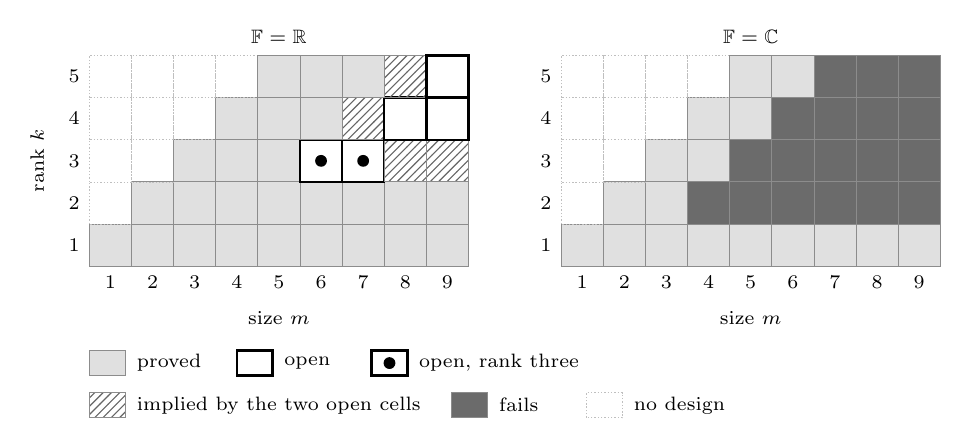
\begin{tikzpicture}[
  x=5.35mm, y=5.35mm,
  every node/.style={font=\scriptsize, inner sep=1pt},
  holds/.style   ={fill=black!12, draw=black!45, line width=0.3pt},
  fails/.style   ={fill=black!58, draw=black!45, line width=0.3pt},
  reduces/.style ={pattern=north east lines, pattern color=black!60,
                   draw=black!45, line width=0.3pt},
  opencell/.style={fill=white, draw=black, line width=0.9pt},
  nodesign/.style={draw=black!25, line width=0.25pt,
                   dash pattern=on 0.5pt off 0.7pt}]

% the cell (m,k) is the unit square with lower left corner (m-1,k-1)
\newcommand{\bcell}[3]{\path[#3] (#1-1,#2-1) rectangle ++(1,1);}
\newcommand{\bfrontier}[2]{%
  \path[opencell] (#1-1,#2-1) rectangle ++(1,1);
  \fill[black] (#1-0.5,#2-0.5) circle[radius=0.75mm];}

% =======================  the real board  ============================
\begin{scope}
  \foreach \m in {1,...,9}{\bcell{\m}{1}{holds}}

  \bcell{1}{2}{nodesign}
  \foreach \m in {2,...,9}{\bcell{\m}{2}{holds}}

  \foreach \m in {1,2}{\bcell{\m}{3}{nodesign}}
  \foreach \m in {3,4,5}{\bcell{\m}{3}{holds}}
  \bfrontier{6}{3}
  \bfrontier{7}{3}
  \foreach \m in {8,9}{\bcell{\m}{3}{reduces}}

  \foreach \m in {1,2,3}{\bcell{\m}{4}{nodesign}}
  \foreach \m in {4,5,6}{\bcell{\m}{4}{holds}}
  \bcell{7}{4}{reduces}
  \foreach \m in {8,9}{\bcell{\m}{4}{opencell}}

  \foreach \m in {1,...,4}{\bcell{\m}{5}{nodesign}}
  \foreach \m in {5,6,7}{\bcell{\m}{5}{holds}}
  \bcell{8}{5}{reduces}
  \bcell{9}{5}{opencell}

  \foreach \m in {1,...,9}{\node[anchor=north] at (\m-0.5,-0.15) {\m};}
  \foreach \k in {1,...,5}{\node[anchor=east]  at (-0.15,\k-0.5) {\k};}
  \node[anchor=north] at (4.5,-1.00) {size $m$};
  \node[rotate=90, anchor=south] at (-1.00,2.5) {rank $k$};
  \node[anchor=south] at (4.5,5.20) {$\FF=\R$};
\end{scope}

% ======================  the complex board  ==========================
\begin{scope}[shift={(11.2,0)}]
  \foreach \m in {1,...,9}{\bcell{\m}{1}{holds}}

  \bcell{1}{2}{nodesign}
  \foreach \m in {2,3}{\bcell{\m}{2}{holds}}
  \foreach \m in {4,...,9}{\bcell{\m}{2}{fails}}

  \foreach \m in {1,2}{\bcell{\m}{3}{nodesign}}
  \foreach \m in {3,4}{\bcell{\m}{3}{holds}}
  \foreach \m in {5,...,9}{\bcell{\m}{3}{fails}}

  \foreach \m in {1,2,3}{\bcell{\m}{4}{nodesign}}
  \foreach \m in {4,5}{\bcell{\m}{4}{holds}}
  \foreach \m in {6,...,9}{\bcell{\m}{4}{fails}}

  \foreach \m in {1,...,4}{\bcell{\m}{5}{nodesign}}
  \foreach \m in {5,6}{\bcell{\m}{5}{holds}}
  \foreach \m in {7,8,9}{\bcell{\m}{5}{fails}}

  \foreach \m in {1,...,9}{\node[anchor=north] at (\m-0.5,-0.15) {\m};}
  \foreach \k in {1,...,5}{\node[anchor=east]  at (-0.15,\k-0.5) {\k};}
  \node[anchor=north] at (4.5,-1.00) {size $m$};
  \node[anchor=south] at (4.5,5.20) {$\FF=\C$};
\end{scope}

% ===========================  legend  ================================
\begin{scope}[shift={(0,-2.60)}]
  \path[holds]    (0,0) rectangle ++(0.85,0.6);
  \node[anchor=west] at (1.05,0.30) {proved};

  \path[opencell] (3.5,0) rectangle ++(0.85,0.6);
  \node[anchor=west] at (4.55,0.30) {open};

  \path[opencell] (6.7,0) rectangle ++(0.85,0.6);
  \fill[black] (7.125,0.30) circle[radius=0.75mm];
  \node[anchor=west] at (7.75,0.30) {open, rank three};
\end{scope}

\begin{scope}[shift={(0,-3.60)}]
  \path[reduces]  (0,0) rectangle ++(0.85,0.6);
  \node[anchor=west] at (1.05,0.30) {implied by the two open cells};

  \path[fails]    (8.6,0) rectangle ++(0.85,0.6);
  \node[anchor=west] at (9.65,0.30) {fails};

  \path[nodesign] (11.8,0) rectangle ++(0.85,0.6);
  \node[anchor=west] at (12.85,0.30) {no design};
\end{scope}

\end{tikzpicture}

  \caption{The decision board.  Rows are the rank $k$, columns the size
  $m$; cells with $m<k$ carry no design.  Over $\R$ the two open cells at
  rank three are $(6,3)$ and $(7,3)$; the hatched region reduces to them
  by Theorem~\ref{thm:window}.  Over $\C$ the answer is $m\le k+1$ for
  every $k\ge2$.}
  \label{fig:board}
\end{figure}

\section{Elementary cases}\label{sec:first}

This section fixes the objects, derives the three counting identities that
every later argument uses, and settles the cases these identities settle
by themselves.  It then isolates, in the form of a lemma and a
counterexample, the exact point at which counting stops working; that
point is what the rest of the paper is about.  Two examples are introduced
here.

\subsection{The objects}

\begin{definition}\label{def:design}
A \emph{weighted design} of size $m$ and rank $k$ over $\FF$ is a pair
$\bigl((g_c)_{c\le m},(t_c)_{c\le m}\bigr)$ with $g_c\in\FF^k$, $t_c>0$
and $\sum_c t_c=1$, satisfying \eqref{eq:parseval}.  For
$C\subseteq\{1,\dots,m\}$ put $\SC:=\sum_{c\in C}g_c^{\vphantom{*}}g_c^{*}$;
the subset $C$ \emph{dominates} if $\SC-I_k\psd0$.  The assertion
$\Gtz(m,k)$ is that every design of size $m$ and rank $k$ over $\R$ admits
a dominating $k$-subset, and $\GtzC(m,k)$ is the same assertion over $\C$.
\end{definition}

Three features of the definition are deliberate.  The vectors are not
required to be distinct or nonzero, so repeated vectors and the zero
vector are admitted.  Excluding them would change the problem and would
not simplify it: a $k$-subset containing two parallel vectors is
rank-deficient and cannot dominate, and it is exactly this mechanism, seen
first in Example~\ref{ex:octa}, that makes selection combinatorial rather
than metric.  The weights are real even over $\C$.
And $\SC$ carries no weights: they enter only through
\eqref{eq:parseval}, which is why domination is preserved by any
operation that keeps the vectors and moves the weights.

Since $g_c^{\vphantom{*}}g_c^{*}\psd0$ for every $c$, adding indices to
$C$ can only increase $\SC$ in the Loewner order; a superset of a
dominating set dominates.  The cardinality restriction
$\lvert C\rvert=k$ is therefore the whole of the problem, and it is
sharp on both sides: fewer than $k$ vectors span a proper subspace and
leave $\SC$ singular, while at $\lvert C\rvert=m$ domination is automatic
(Lemma~\ref{lem:coparseval}).

\begin{lemma}[Lean]\label{lem:span}
The vectors of a design span $\FF^k$.  In particular $k\le m$, and there
is no design with $m<k$.
\end{lemma}

\begin{proof}
Let $u\in\FF^k$ satisfy $\langle u,g_c\rangle=0$ for every $c$.  Pairing
\eqref{eq:parseval} with $u$ gives
\[
  \lVert u\rVert^2\;=\;u^{*}I_ku
  \;=\;\sum_c t_c\,u^{*}g_c^{\vphantom{*}}g_c^{*}u
  \;=\;\sum_c t_c\,\lvert\langle u,g_c\rangle\rvert^2\;=\;0 ,
\]
so $u=0$.  The orthogonal complement of the span is trivial, and a
spanning family in $\FF^k$ has at least $k$ members.
\end{proof}

\subsection{Three counting identities}

Taking the trace of \eqref{eq:parseval} gives the identity on which every
counting argument in the subject rests.

\begin{lemma}[Lean]\label{lem:trace}
$\sum_c s_c=\sum_c t_c\ell_c=k$.  Hence $\max_c \ell_c\ge k$.
\end{lemma}

\begin{proof}
$\tr\bigl(g_c^{\vphantom{*}}g_c^{*}\bigr)=\lVert g_c\rVert^2=\ell_c$, and
$\tr I_k=k$; take traces in \eqref{eq:parseval} term by term.  The
weights are positive and sum to $1$, so $k=\sum_c t_c\ell_c$ is a
weighted mean of the $\ell_c$ and does not exceed their maximum.
\end{proof}

The leverage scores are also bounded above, individually.

\begin{lemma}[Lean]\label{lem:share}
$0\le s_c\le1$ for every $c$.  With Lemma~\ref{lem:trace} the leverage
scores therefore lie in $[0,1]$ and sum to $k$, which gives $m\ge k$ a
second time, with equality only if $s_c=1$ throughout.
\end{lemma}

\begin{proof}
Fix $e$ and separate the $e$-th term of \eqref{eq:parseval}:
\begin{equation}\label{eq:erased}
  I_k-t_e\,g_e^{\vphantom{*}}g_e^{*}
  \;=\;\sum_{c\ne e}t_c\,g_c^{\vphantom{*}}g_c^{*}\;\psd\;0 .
\end{equation}
Evaluating the quadratic form of \eqref{eq:erased} at $g_e$ gives
$0\le\ell_e-t_e\ell_e^2$.  If $\ell_e=0$ then $s_e=0\le1$; otherwise
divide by $\ell_e>0$.
\end{proof}

The third identity compares the unweighted sum over all indices with the
weighted one.

\begin{lemma}[Lean]\label{lem:coparseval}
For every design,
\begin{equation}\label{eq:coparseval}
  S_{\{1,\dots,m\}}-I_k\;=\;\sum_{c}(1-t_c)\,g_c^{\vphantom{*}}g_c^{*} .
\end{equation}
The right-hand side is positive semidefinite, and positive definite as
soon as $m\ge2$.
\end{lemma}

\begin{proof}
Subtract \eqref{eq:parseval} from $\sum_c g_c^{\vphantom{*}}g_c^{*}$.
Each $t_c$ is one summand of a sum of positive numbers equal to $1$, so
$t_c\le1$ and the coefficients $1-t_c$ are nonnegative; a nonnegative
combination of the positive semidefinite matrices
$g_c^{\vphantom{*}}g_c^{*}$ is positive semidefinite.  If $m\ge2$ then
$t_c<1$ for every $c$, since $t_c+t_{c'}\le1$ with $t_{c'}>0$ for any
second index $c'$.  Put $\sigma:=\min_c(1-t_c)/t_c>0$.  Every coefficient
of
\[
  \sum_c\bigl((1-t_c)-\sigma t_c\bigr)\,g_c^{\vphantom{*}}g_c^{*}
  \;=\;\sum_c(1-t_c)\,g_c^{\vphantom{*}}g_c^{*}\;-\;\sigma I_k
\]
is nonnegative by the choice of $\sigma$, the displayed equality being
\eqref{eq:parseval} scaled by $\sigma$.  Hence
$\sum_c(1-t_c)g_c^{\vphantom{*}}g_c^{*}\psd\sigma I_k\pd0$.
\end{proof}

The operator on the right of \eqref{eq:coparseval} is used again in
\S\ref{sec:chart}, where its inverse defines the pivot of a vector and
its positive definiteness supplies the whitening that makes duality
possible.  Nothing else in the present section needs it.

\subsection{The cases that close by counting}

\begin{proposition}[Lean]\label{prop:sizerank}
$\Gtz(k,k)$ and $\GtzC(k,k)$ hold.
\end{proposition}

\begin{proof}
By Lemma~\ref{lem:span} a design of rank $k$ has $m\ge k$ vectors, so
$m=k$ leaves exactly one $k$-subset, namely $\{1,\dots,m\}$, and it
dominates by Lemma~\ref{lem:coparseval}.
\end{proof}

\begin{proposition}[Lean]\label{prop:rankone}
$\Gtz(m,1)$ and $\GtzC(m,1)$ hold for every $m$.
\end{proposition}

\begin{proof}
At $k=1$ the matrices in \eqref{eq:parseval} are scalars and the
condition reads $\sum_c t_c\lvert g_c\rvert^2=1$; this is
Lemma~\ref{lem:trace} at $k=1$.  A weighted mean does not exceed its
maximum, so $\lvert g_{c_0}\rvert^2\ge1$ for some $c_0$, and the
singleton $\{c_0\}$, which has cardinality $k=1$, dominates.
\end{proof}

The two propositions dispose of the cells $m=k$ and $k=1$, and they are the
whole of what the counting identities give directly.  The range
\eqref{eq:elementary} in which the maximal-volume principle already
suffices is larger by exactly one column, $m=k+1$.  That column does reduce
to the scalar mechanism of Proposition~\ref{prop:rankone}, but only after a
change of variables which trades the vectors for the kernel of the
associated projection; it is Theorem~\ref{thm:corankone}, and it is where
the elementary methods end.

The classical statement is the uniform-weight instance, in the following
precise sense.

\begin{proposition}[Lean]\label{prop:classical}
Let $n\ge1$ and let $A\in\FF^{n\times k}$ satisfy $A^{*}A=I_k$.  If
$\Gtz(n,k)$ holds, respectively $\GtzC(n,k)$, then there is an injection
$\iota:\{1,\dots,k\}\to\{1,\dots,n\}$ with
\[
  (A_\iota)^{*}A_\iota^{\vphantom{*}}\;\psd\;\tfrac1n I_k,
  \qquad A_\iota:=\bigl(A_{\iota(1)},\dots,A_{\iota(k)}\bigr)^{*}\!,
\]
where $A_r^{*}$ denotes the $r$-th row of $A$.
\end{proposition}

\begin{proof}
Put $g_r:=\sqrt n\,A_r$ and $t_r:=1/n$.  Then
$\sum_r t_r g_r^{\vphantom{*}}g_r^{*}=\sum_r A_r^{\vphantom{*}}A_r^{*}
=A^{*}A=I_k$, so this is a design of size $n$ and rank $k$.  Let $C$
dominate and let $\iota$ enumerate $C$ in increasing order.  Then
$(A_\iota)^{*}A_\iota^{\vphantom{*}}=\sum_{r\in C}A_r^{\vphantom{*}}A_r^{*}
=\frac1n\SC$, so
\[
  (A_\iota)^{*}A_\iota^{\vphantom{*}}-\tfrac1n I_k
  \;=\;\tfrac1n\bigl(\SC-I_k\bigr)\;\psd\;0 . \qedhere
\]
\end{proof}

At a fixed size the implication goes only this way, so the weighted
statement is formally the stronger of the two; over all sizes they are
equivalent, for the reason given in \S\ref{sec:intro}.

\subsection{Where counting stops}\label{sec:stops}

Domination admits a formulation with no matrices in it.  A $k$-subset $C$
dominates if and only if
\begin{equation}\label{eq:pointwise}
  \sum_{c\in C}\lvert\langle x,g_c\rangle\rvert^2\;\ge\;\lVert x\rVert^2
  \qquad\text{for every }x\in\FF^k ,
\end{equation}
since the left-hand side is the quadratic form of $\SC$ at $x$.  In the
same language \eqref{eq:parseval} says that
$\sum_c t_c\lvert\langle x,g_c\rangle\rvert^2=\lVert x\rVert^2$ for every
$x$: the squared projections of a fixed direction on the vectors of a
design average to the squared length of that direction.  The averaging
mechanism of Proposition~\ref{prop:rankone} therefore survives in full
generality, one direction at a time.

\begin{lemma}[Lean]\label{lem:direction}
For every design and every $x\in\FF^k$ there is an index $c$ with
$\lvert\langle x,g_c\rangle\rvert^2\ge\lVert x\rVert^2$.
\end{lemma}

\begin{proof}
The numbers $\lvert\langle x,g_c\rangle\rvert^2$ have weighted mean
$\lVert x\rVert^2$ by \eqref{eq:parseval}, and a weighted mean with
positive weights summing to $1$ does not exceed the maximum of the
numbers averaged.
\end{proof}

At $k=1$ this is the theorem, because there is only one direction up to
scalars and the witnessing index may be chosen once and for all.  At
$k\ge2$ the witness of Lemma~\ref{lem:direction} depends on $x$, and
\eqref{eq:pointwise} demands a set of $k$ indices that works
simultaneously for every $x$ on a sphere of dimension $k-1$.  No
averaging identity produces such a set: the quantity to be dominated in
\eqref{eq:dominate} is a matrix, and while \eqref{eq:parseval} controls
every scalar linear functional of the family, the least eigenvalue is not
one of them.

The natural scalar relaxation makes the failure quantitative.  If $C$
dominates then all $k$ eigenvalues of $\SC$ are at least $1$, so
\begin{equation}\label{eq:tracetest}
  \tr\SC\;=\;\sum_{c\in C}\ell_c\;\ge\;k .
\end{equation}
This necessary condition is satisfied in every design by a subset that is
found without any work: by Lemma~\ref{lem:trace} some $\ell_{c_0}\ge k$,
and any $k$-subset containing $c_0$ satisfies \eqref{eq:tracetest}
already.  The trace test thus never fails to be satisfiable and never
distinguishes a dominating subset from a non-dominating one.  The
following design, which will also serve as a first illustration of the
cell $(6,3)$, shows how far apart the two can be.

\begin{example}\label{ex:octa}
Let $k=3$, let the six vectors be $\pm\sqrt3\,e_1$, $\pm\sqrt3\,e_2$,
$\pm\sqrt3\,e_3$ and let every weight be $\tfrac16$.  Then
\[
  \sum_c t_c\,g_c^{\vphantom{\mathsf{T}}}g_c\tp
  \;=\;\tfrac16\cdot3\cdot2\sum_{i=1}^{3}e_i^{\vphantom{\mathsf{T}}}e_i\tp\;=\;I_3 ,
\]
so this is a design at $(6,3)$, with $\ell_c=3$ and $s_c=\tfrac12$ for
every $c$, in accordance with Lemmas~\ref{lem:trace} and~\ref{lem:share}.
Every triple satisfies $\tr\SC=9\ge3$.  The triple
$\{\sqrt3e_1,-\sqrt3e_1,\sqrt3e_2\}$ nevertheless has
$\SC=6\,e_1^{\vphantom{\mathsf{T}}}e_1\tp+3\,e_2^{\vphantom{\mathsf{T}}}e_2\tp$, which is
singular in the direction $e_3$ and does not dominate; the triple
$\{\sqrt3e_1,\sqrt3e_2,\sqrt3e_3\}$ has $\SC=3I_3\pd I_3$ and dominates
strictly.  The trace is blind to the difference, and the difference is
which subspaces the chosen vectors miss.
\end{example}

Selection is therefore a combinatorial problem about which directions a
$k$-subset leaves uncovered, constrained by the metric identity
\eqref{eq:parseval}.  The remaining sections develop the two instruments
that address it: a change of coordinates that turns \eqref{eq:dominate}
into a statement about principal blocks of a projection
(\S\ref{sec:chart}), and, when that does not decide the cell, a
variational analysis of the worst design (\S\ref{sec:compactness} and
\S\ref{sec:interior}).

\subsection{The tetrahedron}

In Example~\ref{ex:octa} one triple dominates strictly.  The next design
admits no strict domination at all, and its equality is exact at every
triple.

\begin{example}[Lean]\label{ex:tetra}
Let $k=3$ and take the four vectors
\[
  g_0=(1,1,1),\quad g_1=(1,-1,-1),\quad g_2=(-1,1,-1),\quad g_3=(-1,-1,1)
\]
with equal weights $t_c=\tfrac14$.  Each diagonal entry of
$\sum_c g_c^{\vphantom{\mathsf{T}}}g_c\tp$ is $4$, and each off-diagonal entry is
$1-1-1+1=0$, so
\begin{equation}\label{eq:tetraparseval}
  \sum_{c=0}^{3} g_c^{\vphantom{\mathsf{T}}}g_c\tp\;=\;4I_3,
  \qquad\text{hence}\qquad
  \sum_{c=0}^{3}\tfrac14\,g_c^{\vphantom{\mathsf{T}}}g_c\tp\;=\;I_3 :
\end{equation}
a design at $(4,3)$.  Here $\ell_c=3$ and $s_c=\tfrac34$ for every $c$, so
Lemma~\ref{lem:trace} holds with equal terms, $4\cdot\tfrac34=3=k$, and
$\langle g_i,g_j\rangle=-1$ for $i\ne j$.  The four vectors are the unit
vectors to the vertices of a regular tetrahedron, scaled by $\sqrt3$.

Let $C=\{0,1,2,3\}\setminus\{c_0\}$ be one of the four triples.
Subtracting the omitted term from \eqref{eq:tetraparseval},
\[
  \SC\;=\;4I_3-g_{c_0}^{\vphantom{\mathsf{T}}}g_{c_0}\tp .
\]
The matrix $g_{c_0}^{\vphantom{\mathsf{T}}}g_{c_0}\tp$ has eigenvalue
$\ell_{c_0}=3$ on the line $\R g_{c_0}$ and $0$ on its orthogonal
complement, so
\begin{equation}\label{eq:tetraspec}
  \operatorname{spec}\SC=\{1,4,4\},\qquad \lmin(\SC)=1 .
\end{equation}
Every triple dominates, and every triple dominates with least eigenvalue
exactly $1$.  For $c_0=0$ the certificate is a sum of squares: writing
$x=(x_1,x_2,x_3)$,
\[
  x\tp\bigl(\SC-I_3\bigr)x
  \;=\;3\lVert x\rVert^2-\langle x,g_0\rangle^2
  \;=\;3\sum_i x_i^2-\Bigl(\sum_i x_i\Bigr)^{\!2}
  \;=\;\sum_{i<j}(x_i-x_j)^2 ,
\]
which vanishes exactly on $\R g_0$, the direction omitted from $C$.
\end{example}

The tetrahedron is the smallest design at rank three in which
\eqref{eq:dominate} holds with equality.  It is the equality case
of the corank-one classification: the tie law \eqref{eq:tielaw} of
\S\ref{sec:chart} reads $3\cdot\tfrac14\cdot3=\tfrac94=3-1+\tfrac14$
here.  Splitting its vectors produces extremal designs at every size
$m\ge4$ and rank $3$, which is how the no-margin principle of
\S\ref{sec:ties} reaches the open cells.  Its volume-sampling mixture is
computed in \S\ref{sec:ties} and equals $(x-1)(x-4)^2$, with least root
exactly at the threshold.  And it is the calibration point of the
first-order system of \S\ref{sec:interior}, where the multiplier is
$\Lambda=\tfrac13I_3$ with $v=1$ and each of the four triples carries
multiplier $\tfrac14$.

\begin{figure}[ht]
  \centering
  % The regular tetrahedron design at (4,3), and the spectrum of one of its
% triples.  Orthographic projection of R^3 with azimuth 15 and elevation 70
% degrees, scaled by 1.35cm:
%   X = 1.35(-0.2588 x_1 + 0.9659 x_2)
%   Y = 1.35(-0.9077 x_1 - 0.2432 x_2 + 0.3420 x_3)
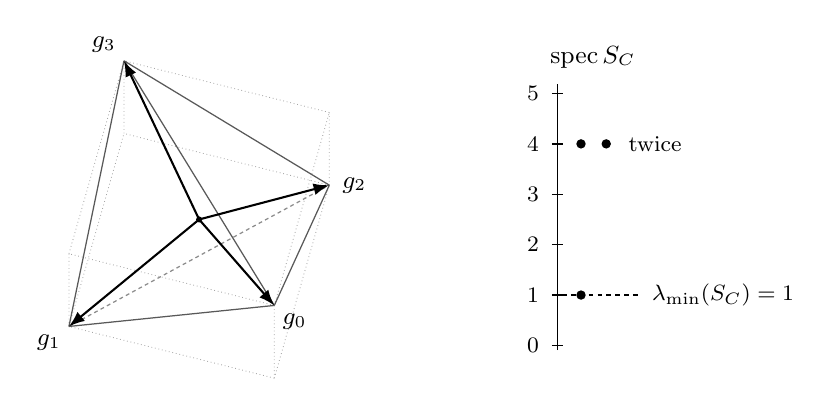
\begin{tikzpicture}[
  x=1cm, y=1cm,
  vec/.style={-{Latex[length=2mm,width=1.5mm]}, line width=0.75pt},
  cube/.style={densely dotted, line width=0.3pt, black!35},
  edge/.style={line width=0.45pt, black!65},
  hidden/.style={line width=0.45pt, black!45, dashed, dash pattern=on 1.4pt off 1.2pt},
  every node/.style={font=\small}]

% ---- the eight vertices of [-1,1]^3 -------------------------------------
\coordinate (ppp) at ( 0.9546,-1.0920);   % g_0 = ( 1, 1, 1)
\coordinate (ppm) at ( 0.9546,-2.0154);   %       ( 1, 1,-1)
\coordinate (pmp) at (-1.6534,-0.4354);   %       ( 1,-1, 1)
\coordinate (pmm) at (-1.6534,-1.3588);   % g_1 = ( 1,-1,-1)
\coordinate (mpp) at ( 1.6534, 1.3588);   %       (-1, 1, 1)
\coordinate (mpm) at ( 1.6534, 0.4354);   % g_2 = (-1, 1,-1)
\coordinate (mmp) at (-0.9546, 2.0154);   % g_3 = (-1,-1, 1)
\coordinate (mmm) at (-0.9546, 1.0920);   %       (-1,-1,-1)
\coordinate (O)   at ( 0,0);

% ---- the cube, as a frame of reference ----------------------------------
\draw[cube] (ppp)--(ppm) (ppp)--(pmp) (ppp)--(mpp)
            (ppm)--(pmm) (ppm)--(mpm) (pmp)--(pmm) (pmp)--(mmp)
            (mpp)--(mpm) (mpp)--(mmp) (pmm)--(mmm) (mpm)--(mmm) (mmp)--(mmm);

% ---- the tetrahedron on the four even-sign vertices ----------------------
\draw[hidden] (pmm)--(mpm);
\draw[edge]   (ppp)--(pmm) (ppp)--(mpm) (mpm)--(mmp) (mmp)--(pmm) (ppp)--(mmp);

% ---- the four vectors of the design -------------------------------------
\draw[vec] (O)--(ppp) node[below right=-1pt] {$g_0$};
\draw[vec] (O)--(pmm) node[below left=-1pt]  {$g_1$};
\draw[vec] (O)--(mpm) node[right=1pt]        {$g_2$};
\draw[vec] (O)--(mmp) node[above left=-1pt]  {$g_3$};
\fill (O) circle (1.1pt);

% ---- the spectrum of a triple -------------------------------------------
% the eigenvalue lambda is drawn at height  -1.6 + 0.64 lambda
\begin{scope}[shift={(4.55,0)}]
  \draw[line width=0.5pt] (0,-1.66)--(0,1.72);
  \foreach \l/\lab in {0/0,1/1,2/2,3/3,4/4,5/5}{
    \pgfmathsetmacro{\hh}{-1.6+0.64*\l}
    \draw[line width=0.5pt] (-0.07,\hh)--(0.07,\hh);
    \node[anchor=east, font=\footnotesize] at (-0.11,\hh) {\lab};
  }
  % the threshold: the eigenvalue of I_3
  \draw[dashed, dash pattern=on 1.7pt off 1.5pt, line width=0.5pt]
        (0.06,-0.96)--(1.05,-0.96);
  \node[anchor=west, font=\footnotesize] at (1.08,-0.96) {$\lmin(\SC)=1$};
  % the three eigenvalues 1, 4, 4
  \fill (0.30,-0.96) circle (1.7pt);
  \fill (0.30, 0.96) circle (1.7pt);
  \fill (0.62, 0.96) circle (1.7pt);
  \node[anchor=west, font=\footnotesize] at (0.78,0.96) {twice};
  \node[anchor=south] at (0.45,1.80) {$\operatorname{spec}\SC$};
\end{scope}

\end{tikzpicture}

  \caption{The design of Example~\ref{ex:tetra}: four vectors to the
  vertices of a regular tetrahedron, drawn inside the cube whose even-sign
  vertices they are.  Every triple omits one vector and has spectrum
  $\{1,4,4\}$ by \eqref{eq:tetraspec}, so the least eigenvalue sits
  exactly on the threshold.}
  \label{fig:tetrahedron}
\end{figure}

\section{The projection chart}\label{sec:chart}

Absorbing the weights into the vectors replaces a design by a projection
on the index space, and replaces the domination condition
\eqref{eq:dominate} by a comparison between a principal block of that
projection and a diagonal matrix.

Throughout, $k\ge1$ and $m\ge k$; the second inequality is
Lemma~\ref{lem:span}.  For an index set $C$ of size $r$,
listed in increasing order, $M_C$ denotes the $r\times k$ matrix whose
rows are $g_c\adj$, $c\in C$, and
\[
  \Gram_C\;:=\;M_C^{\vphantom{\mathsf{H}}}M_C\adj
  \;=\;\bigl(\langle g_c,g_d\rangle\bigr)_{c,d\in C}
\]
their Gram matrix.  The two products of $M_C$ carry different
information:
\begin{equation}\label{eq:twoproducts}
  M_C\adj M_C^{\vphantom{\mathsf{H}}}\;=\;\sum_{c\in C}g_c^{\vphantom{\mathsf{H}}}g_c\adj
  \;=\;\SC \quad (k\times k),
  \qquad
  M_C^{\vphantom{\mathsf{H}}}M_C\adj\;=\;\Gram_C \quad (r\times r).
\end{equation}
Both identities are the definition of matrix multiplication read in the
two possible orders.

\subsection{Construction}\label{sec:chartconstruction}

Put
\[
  v_c\;:=\;\sqrt{t_c}\,g_c\in\FF^{k},
\]
and let $V$ be the $m\times k$ matrix whose $c$-th row is $v_c\adj$; thus
$V=\diag(\sqrt{t_1},\dots,\sqrt{t_m})\,M_{\{1,\dots,m\}}$.  The Parseval
condition \eqref{eq:parseval} is exactly the orthonormality of the
columns of $V$:
\begin{equation}\label{eq:isometry}
  V\adj V\;=\;\sum_{c}v_c^{\vphantom{\mathsf{H}}}v_c\adj
  \;=\;\sum_c t_c\,g_c^{\vphantom{\mathsf{H}}}g_c\adj\;=\;I_k .
\end{equation}
Accordingly
\begin{equation}\label{eq:chart}
  P\;:=\;VV\adj
\end{equation}
is a matrix on the \emph{index} space $\FF^m$.  Write
$D:=\diag(t_1,\dots,t_m)$ and
\begin{equation}\label{eq:chartgap}
  W\;:=\;P-D .
\end{equation}
The pair $(P,t)$ is the \emph{chart} of the design and $W$ its
\emph{gap}.

\begin{proposition}[Lean]\label{prop:chartid}
$P$ is the orthogonal projection onto the column space of $V$, of rank
$k$, and
\[
  P_{cd}=\sqrt{t_ct_d}\,\langle g_c,g_d\rangle,
  \qquad P_{cc}=s_c,\qquad \tr P=k .
\]
Consequently $W_{cc}=t_c(\ell_c-1)$ and $\sum_c W_{cc}=k-1$.
\end{proposition}

\begin{proof}
$P\adj=(VV\adj)\adj=VV\adj=P$, and, by \eqref{eq:isometry},
$P^2=V(V\adj V)V\adj=VIV\adj=P$.  A Hermitian idempotent is the orthogonal
projection onto its range; that range lies in the column space of $V$, and
$VV\adj V=V(V\adj V)=V$ puts the column space back inside it, a second use
of \eqref{eq:isometry}.  The rank of $P$ is therefore the rank of $V$,
which is $k$ because $V\adj V=I_k$.  The entries are
$P_{cd}=\langle v_c,v_d\rangle=\sqrt{t_ct_d}\langle g_c,g_d\rangle$; at
$c=d$ this is $t_c\ell_c=s_c$.  Finally
$\tr P=\tr(VV\adj)=\tr(V\adj V)=\tr I_k=k$.  The diagonal of $W$ is
$s_c-t_c=t_c(\ell_c-1)$, and $\sum_c(s_c-t_c)=k-1$ by
Lemma~\ref{lem:trace}.
\end{proof}

\begin{lemma}\label{lem:realize}
Fix $m$, $k$ and a weight vector $t$ with $t_c>0$ and $\sum_ct_c=1$.  The
map sending a design with weight vector $t$ to its chart $P$ is a
bijection from the set of such designs modulo the action
$g_c\mapsto Ug_c$ of the unitary group of $\FF^k$ onto the set of
orthogonal projections of rank $k$ on $\FF^m$.
\end{lemma}

\begin{proof}
Let $P$ be an orthogonal projection of rank $k$ and let $V$ be the
$m\times k$ matrix whose columns are an orthonormal basis of the range of
$P$; then $V\adj V=I_k$ and $VV\adj=P$.  Writing $v_c\adj$ for the $c$-th
row of $V$ and setting $g_c:=t_c^{-1/2}v_c$ produces a family with
$\sum_ct_cg_c^{\vphantom{\mathsf{H}}}g_c\adj=\sum_cv_c^{\vphantom{\mathsf{H}}}v_c\adj
=V\adj V=I_k$, a design with weight vector $t$ and chart $P$.  If two
designs with weight vector $t$ have the same chart, their matrices $V$
and $V'$ have the same column space and orthonormal columns, so their
columns are two orthonormal bases of one $k$-dimensional space and
$V'=VU$ for a unitary $U$ of $\FF^k$, whence $g'_c=U\adj g_c$; conversely
replacing $g_c$ by $Ug_c$ replaces $V$ by $VU\adj$ and leaves
$P=VV\adj$ unchanged.
\end{proof}

\begin{remark}\label{rem:frames}
In frame language \eqref{eq:isometry} says that $(v_c)_{c\le m}$ is a
Parseval frame for $\FF^k$ and $P$ is the associated projection of the
ambient $\FF^m$ onto it \cite{CasazzaKutyniok2013}.  The classical
problem is the uniform slice: for $t_c\equiv1/n$ and $g_c:=\sqrt n\,a_c$,
where $a_c\adj$ is the $c$-th row of a matrix $A$ with $A\adj A=I_k$, the
factor $\sqrt n$ in the vectors cancels the factor $1/n$ in the weights
and $P=AA\adj$; domination of $C$ reads
$\sum_{c\in C}a_c^{\vphantom{\mathsf{H}}}a_c\adj\psd n^{-1}I_k$, which is the
row-selection problem of \cite{GTZ1997}.  In
that slice $D=n^{-1}I$ and the chart criterion below is the condition
$\lmin(P[C])\ge1/n$ used in \cite{Nesterenko2023,Nesterenko2025}.  The
general weight vector is new: $D$ is then a genuine diagonal, and the
comparison is Loewner rather than scalar.
\end{remark}

\subsection{The criterion}\label{sec:criterion}

Two steps separate $\SC$ from the block $W[C]$: a congruence by a
positive diagonal, which holds at every selection size, and an exchange
of the two products in \eqref{eq:twoproducts}, which needs
$\lvert C\rvert=k$.

\begin{lemma}[Lean]\label{lem:congruence}
For every index set $C$ of size $r$,
\begin{equation}\label{eq:congruence}
  W[C]\;=\;\diag(\sqrt{t_c})_{c\in C}\;
  \bigl(\Gram_C-I_r\bigr)\;\diag(\sqrt{t_c})_{c\in C},
\end{equation}
and therefore $W[C]\psd0$ if and only if $\Gram_C\psd I_r$.
\end{lemma}

\begin{proof}
Entrywise, for $c,d\in C$,
\[
  W[C]_{cd}
  \;=\;P_{cd}-t_c\delta_{cd}
  \;=\;\sqrt{t_ct_d}\,\langle g_c,g_d\rangle-\sqrt{t_ct_d}\,\delta_{cd}
  \;=\;\sqrt{t_ct_d}\,\bigl(\Gram_C-I_r\bigr)_{cd},
\]
where the middle step uses $\sqrt{t_ct_d}\,\delta_{cd}=t_c\delta_{cd}$.
This is \eqref{eq:congruence}.  The matrix $B:=\diag(\sqrt{t_c})_{c\in C}$
is invertible because every $t_c>0$, and for invertible $B$ one has
$X\psd0$ if and only if $B\adj XB\psd0$: the substitutions $x\mapsto Bx$
and $x\mapsto B^{-1}x$ carry each quadratic form to the other.
\end{proof}

\begin{lemma}[Lean]\label{lem:flip}
Let $X$ be a matrix over $\FF$, of any shape.  Then
\[
  I-X\adj X\psd0
  \quad\Longleftrightarrow\quad
  I-XX\adj\psd0 .
\]
If $M$ is square, then $M\adj M\psd I$ if and only if $MM\adj\psd I$.
\end{lemma}

\begin{proof}
Both conditions say that a map does not increase length: $I-X\adj X\psd0$
says $\lVert Xu\rVert\le\lVert u\rVert$ for every $u$, and $I-XX\adj\psd0$
says $\lVert X\adj w\rVert\le\lVert w\rVert$ for every $w$.  The first
statement therefore asserts that $X$ is a contraction if and only if
$X\adj$ is, and being symmetric in the two it needs only one implication.

Let $X$ be a contraction and fix $w$.  Then
$\lVert X\adj w\rVert^{2}=\langle w,XX\adj w\rangle$; applying
Cauchy--Schwarz to that inner product and then the hypothesis at
$u=X\adj w$,
\[
  \lVert X\adj w\rVert^4
  \;=\;\langle w,X(X\adj w)\rangle^2
  \;\le\;\lVert w\rVert^2\,\lVert X(X\adj w)\rVert^2
  \;\le\;\lVert w\rVert^2\,\lVert X\adj w\rVert^2 .
\]
If $X\adj w=0$ the bound $\lVert X\adj w\rVert\le\lVert w\rVert$ is
immediate; otherwise divide by $\lVert X\adj w\rVert^{2}$.

The second statement carries the opposite inequality: $M\adj M\psd I$ says
$\lVert Mu\rVert\ge\lVert u\rVert$, so $M$ expands rather than contracts.
Inverting reduces it to the case just proved.  An expansion is injective,
so the square matrix $M$ is invertible, and substituting $u=M^{-1}w$ gives
$\lVert w\rVert\ge\lVert M^{-1}w\rVert$: the inverse is a contraction.  By
the first statement its adjoint $(M^{-1})\adj=(M\adj)^{-1}$ is a
contraction as well, and
substituting $w=M\adj u$ in
$\lVert (M\adj)^{-1}w\rVert\le\lVert w\rVert$ returns
$\lVert u\rVert\le\lVert M\adj u\rVert$, which is $MM\adj\psd I$.  The
converse exchanges $M$ and $M\adj$.
\end{proof}

\begin{lemma}[Lean]\label{lem:chart}
For every $k$-subset $C$,
\[
  \SC\psd I_k \quad\Longleftrightarrow\quad W[C]\psd 0 .
\]
\end{lemma}

\begin{proof}
For $\lvert C\rvert=k$ the matrix $M_C$ is square, so
Lemma~\ref{lem:flip} applies to \eqref{eq:twoproducts} and gives
$\SC=M_C\adj M_C^{\vphantom{\mathsf{H}}}\psd I_k$ if and only if
$\Gram_C=M_C^{\vphantom{\mathsf{H}}}M_C\adj\psd I_k$.  By
Lemma~\ref{lem:congruence} the latter is $W[C]\psd0$.
\end{proof}

The problem therefore reads: \emph{some $k\times k$ principal block of a
rank-$k$ orthogonal projection dominates the corresponding block of a
positive diagonal matrix of trace one}.

The weights enter only through $D$, so the projection and the weights may
be varied independently, and $W[C]\psd0$ is a closed condition in both
arguments.  The compactification of \S\ref{sec:compactness} rests on both
facts.  Figure~\ref{fig:chart} traces the construction.

\begin{figure}[ht]
  \centering
  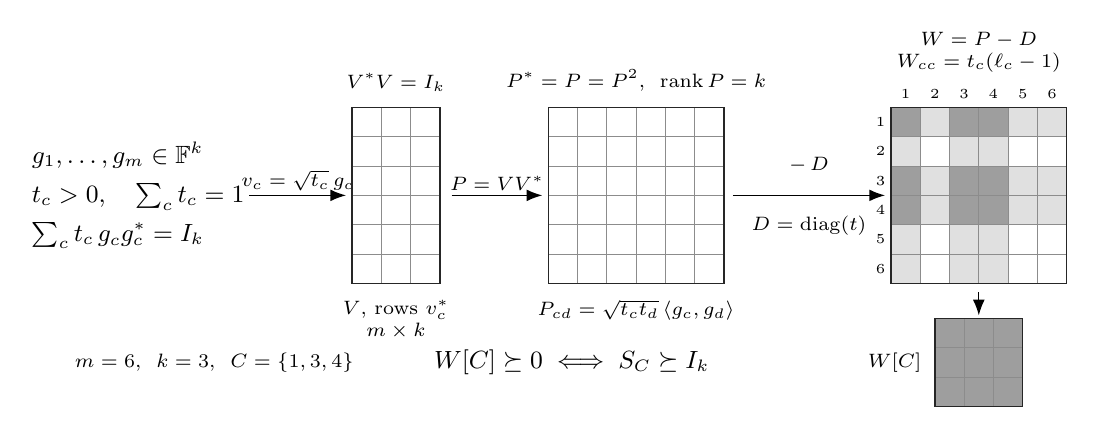
\begin{tikzpicture}[
  x=3.72mm, y=3.72mm,
  every node/.style={inner sep=1.5pt},
  cellline/.style={draw=black!45, line width=0.25pt},
  border/.style  ={draw=black!85, line width=0.5pt},
  ar/.style      ={-{Latex[length=2mm,width=1.5mm]}, line width=0.5pt}]

% a grid of #3 columns and #4 rows with lower left corner (#1,#2)
\newcommand{\gridframe}[4]{%
  \foreach \gi in {0,...,#3}{\draw[cellline] (#1+\gi,#2) -- (#1+\gi,#2+#4);}
  \foreach \gj in {0,...,#4}{\draw[cellline] (#1,#2+\gj) -- (#1+#3,#2+\gj);}
  \draw[border] (#1,#2) rectangle (#1+#3,#2+#4);}
% cell in row #2 from the top and column #3 of the six by six matrix whose
% lower left corner is (#1,-3), filled with #4
\newcommand{\wfill}[4]{\path[fill=#4] (#1+#3-1,3-#2) rectangle ++(1,1);}

% -------------------------- the design -------------------------------
\node[align=left, font=\small] at (3.2,0)
  {$g_1,\dots,g_m\in\FF^{k}$\\[3pt]
   $t_c>0,\quad\textstyle\sum_c t_c=1$\\[3pt]
   $\textstyle\sum_c t_c\,g_c^{\vphantom{*}}g_c^{*}=I_k$};

\draw[ar] (7.0,0) -- node[above, font=\scriptsize] {$v_c=\sqrt{t_c}\,g_c$} (10.3,0);

% ----------------------------- V -------------------------------------
\gridframe{10.5}{-3}{3}{6}
\node[font=\scriptsize, anchor=south] at (12.0,3.4) {$V^{*}V=I_k$};
\node[font=\scriptsize, align=center, anchor=north] at (12.0,-3.4)
  {$V$, rows $v_c^{*}$\\ $m\times k$};

\draw[ar] (13.9,0) -- node[above, font=\scriptsize] {$P=VV^{*}$} (17.0,0);

% ----------------------------- P -------------------------------------
\gridframe{17.2}{-3}{6}{6}
\node[font=\scriptsize, anchor=south] at (20.2,3.4) {$P^{*}=P=P^{2}$, \ $\rk P=k$};
\node[font=\scriptsize, anchor=north] at (20.2,-3.4)
  {$P_{cd}=\sqrt{t_ct_d}\,\langle g_c,g_d\rangle$};

\draw[ar] (23.5,0) -- (28.7,0);
\node[font=\scriptsize] at (26.1,1.05) {$-\,D$};
\node[font=\scriptsize] at (26.1,-1.05) {$D=\diag(t)$};

% ----------------------------- W -------------------------------------
% the selected rows and columns are C = {1,3,4}
\foreach \r in {1,3,4}{\foreach \c in {1,...,6}{\wfill{28.9}{\r}{\c}{black!12}}}
\foreach \c in {1,3,4}{\foreach \r in {1,...,6}{\wfill{28.9}{\r}{\c}{black!12}}}
\foreach \r in {1,3,4}{\foreach \c in {1,3,4}{\wfill{28.9}{\r}{\c}{black!38}}}
\gridframe{28.9}{-3}{6}{6}
\foreach \c in {1,...,6}{\node[font=\tiny] at (28.4+\c,3.45) {\c};}
\foreach \r in {1,...,6}{\node[font=\tiny] at (28.55,3.5-\r) {\r};}
\node[font=\scriptsize, align=center, anchor=south] at (31.9,4.05)
  {$W=P-D$\\ $W_{cc}=t_c(\ell_c-1)$};

% -------------------- the selection window extracted ------------------
\draw[ar] (31.9,-3.3) -- (31.9,-4.1);
\foreach \r in {1,2,3}{\foreach \c in {1,2,3}{%
  \path[fill=black!38] (30.4+\c-1,-7.2+3-\r) rectangle ++(1,1);}}
\gridframe{30.4}{-7.2}{3}{3}
\node[font=\scriptsize, anchor=east] at (30.1,-5.7) {$W[C]$};

\node[font=\small] at (18.0,-5.7) {$W[C]\psd0\iff\SC\psd I_k$};
\node[font=\scriptsize] at (5.8,-5.7) {$m=6$, \ $k=3$, \ $C=\{1,3,4\}$};

\end{tikzpicture}

  \caption{The chart, at $m=6$, $k=3$ and $C=\{1,3,4\}$.  The design data
  pass through the isometry $V$ of \eqref{eq:isometry} to the projection
  $P=VV\adj$ of \eqref{eq:chart} and the gap $W=P-D$ of
  \eqref{eq:chartgap}.  Selecting $C$ is taking a principal block, and
  Lemma~\ref{lem:chart} identifies its semidefiniteness with domination.}
  \label{fig:chart}
\end{figure}

\begin{remark}\label{rem:size}
The equivalence of Lemma~\ref{lem:chart} depends on the hypothesis
$\lvert C\rvert=k$.  Domination is the $k\times k$ statement
$M_C\adj M_C\psd I_k$, while the block condition is the
$r\times r$ statement $M_C^{\vphantom{\mathsf{H}}}M_C\adj\psd I_r$ with
$r=\lvert C\rvert$.  For $r<k$ the left-hand matrix has rank at most
$r<k$ and can never dominate $I_k$, while the block condition is
unconstrained; for $r>k$ the block matrix has rank at most $k<r$ and
never dominates $I_r$, while $\SC$ may.  Both failures are rank effects,
and $r=k$ is the only size at which the equivalence has content in both
directions.
\end{remark}

Taking determinants in \eqref{eq:congruence} converts the criterion into
an exact scalar test, one principal minor at a time.

\begin{corollary}[Lean]\label{cor:minor}
For every index set $C$,
\[
  \det W[C]\;=\;\Bigl(\prod_{c\in C}t_c\Bigr)\,\det(\Gram_C-I).
\]
\end{corollary}

The factor is the square of $\det\diag(\sqrt{t_c})_{c\in C}$ and is
strictly positive, so $W[C]$ and $\Gram_C-I$ have the same principal
minors up to positive factors and are semidefinite together, minor by
minor.  Over the rationals the minors decide the question by exact
arithmetic, with no eigenvalue computation and no genericity assumption.

The design below has four dominating pairs of six, one of them with slack
zero.

\begin{example}\label{ex:chartworked}
Over $\R$ at $(m,k)=(4,2)$ take
\[
  g_0=(\sqrt2,0),\qquad
  g_1=\tfrac1{\sqrt3}(2,1),\qquad
  g_2=\tfrac1{\sqrt3}(1,-2),\qquad
  g_3=(0,2)
\]
with weights $t=\tfrac19(2,3,3,1)$, which are positive and sum to one.
The four terms of \eqref{eq:parseval} are
\[
  \tfrac19\begin{pmatrix}4&0\\0&0\end{pmatrix},\qquad
  \tfrac19\begin{pmatrix}4&2\\2&1\end{pmatrix},\qquad
  \tfrac19\begin{pmatrix}1&-2\\-2&4\end{pmatrix},\qquad
  \tfrac19\begin{pmatrix}0&0\\0&4\end{pmatrix},
\]
of sum $\tfrac19\begin{psmallmatrix}9&0\\0&9\end{psmallmatrix}=I_2$: a
design at $(4,2)$.  The leverages are
$\ell=(2,\tfrac53,\tfrac53,4)$ and the leverage scores
$s_c=t_c\ell_c=\tfrac19(4,5,5,4)$, which sum to $2=k$
(Lemma~\ref{lem:trace}).

Whitening clears the radicals.  With $v_c=\sqrt{t_c}\,g_c$,
\[
  V=\tfrac13\begin{pmatrix}2&0\\2&1\\1&-2\\0&2\end{pmatrix},
\]
and the two columns of $3V$ have squared lengths $4+4+1+0=9$ and
$0+1+4+4=9$ and inner product $0+2-2+0=0$.  Dividing by $9$ gives
$V\adj V=I_2$, which is \eqref{eq:isometry}.  The atoms carry $\sqrt2$ and
$\sqrt3$ and the chart carries neither:
\[
  P=VV\adj=\tfrac19\begin{pmatrix}
    4&4&2&0\\ 4&5&0&2\\ 2&0&5&-4\\ 0&2&-4&4\end{pmatrix}.
\]
Idempotency is ten integer identities.  Write $r_c$ for the $c$-th row of
$9P$.  Then $\bigl((9P)^2\bigr)_{cd}=\langle r_c,r_d\rangle$, and $P^2=P$
asks that this equal $9\,(9P)_{cd}$.  The ten inner products are
\[
  \begin{array}{llll}
  \langle r_0,r_0\rangle=36, & \langle r_0,r_1\rangle=36,
    & \langle r_0,r_2\rangle=18, & \langle r_0,r_3\rangle=0,\\[2pt]
  \langle r_1,r_1\rangle=45, & \langle r_1,r_2\rangle=0,
    & \langle r_1,r_3\rangle=18, & \langle r_2,r_2\rangle=45,\\[2pt]
  \langle r_2,r_3\rangle=-36, & \langle r_3,r_3\rangle=36,
  \end{array}
\]
which are $9$ times $4,4,2,0,5,0,2,5,-4,4$, the corresponding entries of
$9P$.  The trace is $\tfrac19(4+5+5+4)=2=k$ and the diagonal is $s$, as
Proposition~\ref{prop:chartid} says.  Subtracting $D=\diag(t)$,
\[
  W=\tfrac19\begin{pmatrix}
    2&4&2&0\\ 4&2&0&2\\ 2&0&2&-4\\ 0&2&-4&3\end{pmatrix},
  \qquad
  W_{cc}=t_c(\ell_c-1)=\tfrac19(2,2,2,3),
  \qquad \textstyle\sum_cW_{cc}=1=k-1 .
\]

Now take the six blocks.  Every $W_{cc}$ is positive, so a $2\times2$
principal block of $W$ is positive semidefinite precisely when its
determinant is nonnegative and positive definite precisely when that
determinant is positive:
\[
  \begin{array}{r|rrrrrr}
  C & \{0,1\} & \{0,2\} & \{0,3\} & \{1,2\} & \{1,3\} & \{2,3\}\\[2pt]
  81\det W[C] & -12 & 0 & 6 & 4 & 2 & -10
  \end{array}
\]
By Lemma~\ref{lem:chart} four pairs dominate, three of them strictly,
while $\{0,1\}$ and $\{2,3\}$ do not.

Corollary~\ref{cor:minor} checks each entry a second way.  For a pair,
$\det(\Gram_C-I)=(\ell_c-1)(\ell_d-1)-\lvert\langle
g_c,g_d\rangle\rvert^2$, in which the inner product enters squared, so the
radicals cancel there too.  Here $\ell_c-1=(1,\tfrac23,\tfrac23,3)$, and
the six squared inner products, in the order of the table below, are
$\tfrac83$, $\tfrac23$, $0$, $0$, $\tfrac43$, $\tfrac{16}3$, whence
\[
  \begin{array}{r|rrrrrr}
  C & \{0,1\} & \{0,2\} & \{0,3\} & \{1,2\} & \{1,3\} & \{2,3\}\\[2pt]
  \prod_{c\in C}t_c
    & \tfrac2{27} & \tfrac2{27} & \tfrac2{81}
    & \tfrac19 & \tfrac1{27} & \tfrac1{27}\\[4pt]
  \det(\Gram_C-I) & -2 & 0 & 3 & \tfrac49 & \tfrac23 & -\tfrac{10}3
  \end{array}
\]
The six products of the last two rows, multiplied by $81$, return the
minors of the first table.  At $\{0,3\}$ the product is
$\tfrac2{81}\cdot3=\tfrac6{81}$ and $81\cdot\tfrac6{81}=6$.

The pair with determinant zero is $\{0,2\}$, where
\[
  \SC=\begin{pmatrix}2&0\\0&0\end{pmatrix}
     +\tfrac13\begin{pmatrix}1&-2\\-2&4\end{pmatrix}
     =\begin{pmatrix}\tfrac73&-\tfrac23\\[3pt]
                     -\tfrac23&\tfrac43\end{pmatrix} .
\]
The matrix $\SC-I_2$ has determinant $0$ and trace $\tfrac53$, so
$\operatorname{spec}\SC=\{1,\tfrac83\}$ and $\lmin(\SC)=1$.  Its kernel is
spanned by $(1,2)$, and at $x=\tfrac1{\sqrt5}(1,2)$ the pointwise form
\eqref{eq:pointwise} reads $\tfrac25+\tfrac35=1$: the pair covers that one
direction with nothing to spare and every other direction strictly.

The two failures need no determinant.  A dominating pair has
$(\SC)_{jj}\ge1$ at every $j$, and
\[
  S_{\{0,1\}}=\begin{pmatrix}\tfrac{10}3&\tfrac23\\[3pt]
                             \tfrac23&\tfrac13\end{pmatrix},
  \qquad
  S_{\{2,3\}}=\begin{pmatrix}\tfrac13&-\tfrac23\\[3pt]
                             -\tfrac23&\tfrac{16}3\end{pmatrix}
\]
fall to $\tfrac13$ at $e_2$ and at $e_1$.  On the chart side that shortcut
is unavailable, since every $W_{cc}$ is positive.  Over the six pairs
$\max_C\lmin(\SC)=2$, attained at $\{0,3\}$, where $\SC=\diag(2,4)$.
\end{example}

The six pairs are the edges of $K_4$ on the four indices.
Figure~\ref{fig:chartworked} labels each edge with its minor, and the two
failing pairs come out opposite edges.

\begin{figure}[ht]
  \centering
  % The chart of one real design at (4,2), carried through and read off at all
% six pairs.  Three panels: the pipeline g -> V -> P -> W with the matrices in
% it, the four atoms against the unit circle of F^2 = R^2, and the six pairs as
% the edges of K_4 labelled by 81 det W[C].
%
% PROJECTION.  The atom panel is a plane figure and carries no projection of a
% higher-dimensional space: the map is the identity of R^2 scaled by 1.05cm,
%   X = 1.05 x_1,   Y = 1.05 x_2,
% so no viewing normal and no visibility rule are needed and no line is hidden.
% Every coordinate in that panel is that pair.  The K_4 panel is a graph
% drawing on the square derived below, and the reading block is a stack of
% rows.  Every coordinate in all three carries its exact source in a trailing
% comment.
%
% THE DESIGN, exactly.  Over R, m = 4, k = 2.
%   g_0 = (sqrt2, 0)        t_0 = 2/9    ell_0 = 2      s_0 = 4/9
%   g_1 = (2, 1)/sqrt3      t_1 = 3/9    ell_1 = 5/3    s_1 = 5/9
%   g_2 = (1,-2)/sqrt3      t_2 = 3/9    ell_2 = 5/3    s_2 = 5/9
%   g_3 = (0, 2)            t_3 = 1/9    ell_3 = 4      s_3 = 4/9
% The weights are positive and sum to one, and sum_c t_c g_c g_c^T = I_2 over
% the rationals: the four rank-one terms are (2/9)[[2,0],[0,0]],
% (1/9)[[4,2],[2,1]], (1/9)[[1,-2],[-2,4]] and (1/9)[[0,0],[0,4]], of sum
% (1/9)[[9,0],[0,9]].  The leverage scores sum to 4/9+5/9+5/9+4/9 = 2 = k.
% Whitening gives v_c = sqrt(t_c) g_c = (1/3)(2,0), (1/3)(2,1), (1/3)(1,-2),
% (1/3)(0,2), whence the rational V, P = V V^T and W = P - diag(t) printed in
% the pipeline.  81 det W[C] over the six pairs is -12, 0, +6, +4, +2, -10 in
% the order {0,1}, {0,2}, {0,3}, {1,2}, {1,3}, {2,3}.
%
% ELLIPSE FRAME.  For a pair C the set {x : x^T S_C x = 1} is an ellipse with
% semi-axes 1/sqrt(lambda) along the eigenvectors of S_C, and S_C >= I holds
% exactly when that ellipse lies in the closed unit disc.  At C = {0,2},
% S_C = [[7/3,-2/3],[-2/3,4/3]] has spectrum {1, 8/3}, so the semi-axes are 1
% and sqrt(3/8) = 0.6123724, the long one along the eigenvector (1,2)/sqrt5 at
% atan2(2,1) = 63.4349 degrees, and the ellipse touches the unit circle at the
% two points +-(1,2)/sqrt5 = +-(0.4472136, 0.8944272).  Only this ellipse is
% drawn.  The two failing pairs have long semi-axis 2.0163 at C = {2,3} and
% 2.2830 at C = {0,1}, and bounding half-extents sqrt((S_C^-1)_jj) of (2, 1/2)
% and (1/sqrt2, sqrt5) = (0.7071068, 2.2360680) against the 1.05 of the unit
% circle, so each widens the plate in one direction; and the K_4 panel already
% records the sign that decides them.
%
% K_4 FRAME.  The four indices sit at the corners of a square of half-side
% 1.05cm in the cyclic order 0, 1, 2, 3, so that the complement map C -> C^c on
% pairs is the opposite-edge map: {0,1} against {2,3}, {0,3} against {1,2}, and
% the two diagonals {0,2} against {1,3}.  That is the pairing thm:duality uses
% at this self-dual cell; figures/dualworked.tex runs the same pairing down its
% table, C in the first column against E = C^c in the third.  Edge labels sit
% at parameter 0.28 from the first endpoint on the two diagonals and at the
% midpoint on the four sides; the open marker on {0,2} sits at parameter 0.75
% along it, clear of the crossing.  The tangency label names the line through
% the two marks and so carries the sign +-, as the caption does.
%
% DISCLOSED: this design is new to the paper and no Lean declaration mentions
% it.  Every number above and below was computed in exact arithmetic outside
% the assistant -- rational for the chart, the gap and the six minors,
% algebraic for the atoms, the ellipse and the tangency, whose decimals in the
% body are truncations of those exact values.  What is mechanized is the
% machinery it instantiates,
% not the instance: the chart identities of prop:chartid, the criterion of
% lem:chart, and the minor identity of cor:minor.
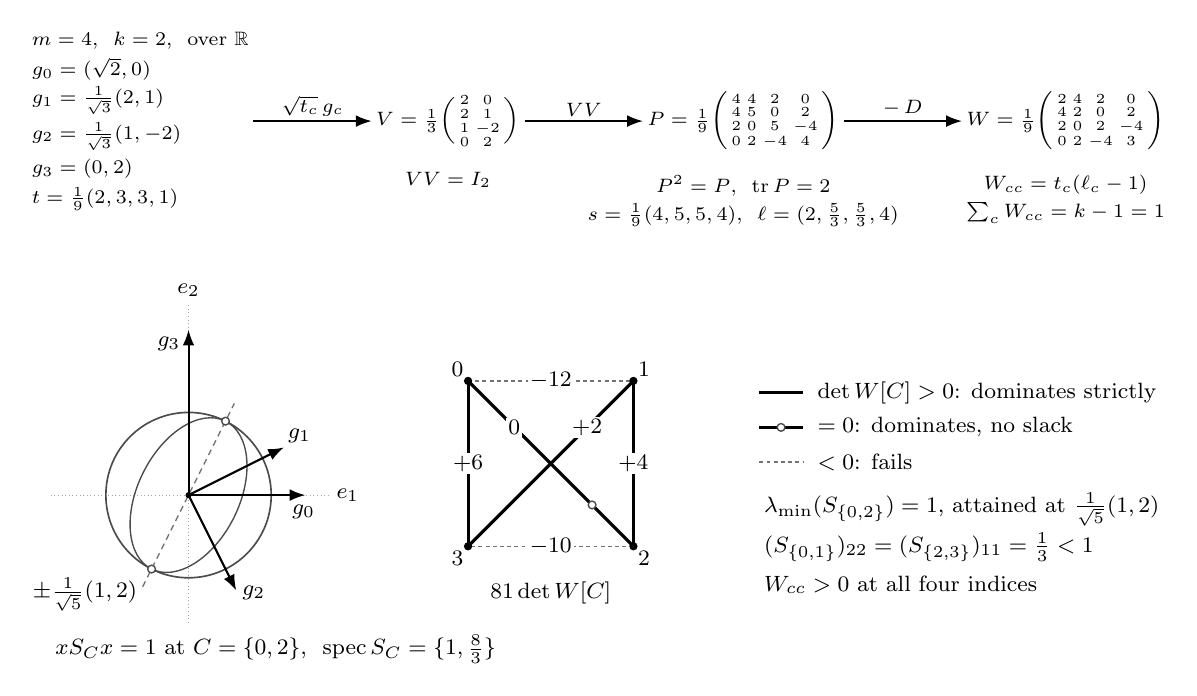
\begin{tikzpicture}[
  x=1cm, y=1cm,
  ar/.style     ={-{Latex[length=2mm,width=1.5mm]}, line width=0.5pt},
  vec/.style    ={-{Latex[length=2mm,width=1.5mm]}, line width=0.75pt},
  rim/.style    ={line width=0.6pt, black!70},
  lev/.style    ={line width=0.5pt, black!70},
  frame/.style  ={densely dotted, line width=0.3pt, black!35},
  tight/.style  ={line width=0.5pt, black!55, dashed,
                  dash pattern=on 2.2pt off 1.6pt},
  win/.style    ={line width=1.1pt},
  lose/.style   ={line width=0.55pt, black!55, dashed,
                  dash pattern=on 1.4pt off 1.2pt},
  tag/.style    ={font=\footnotesize, fill=white, inner sep=0.8pt},
  blk/.style    ={inner sep=1.5pt, font=\scriptsize},
  every node/.style={inner sep=1.5pt, font=\small}]

% =========================== the pipeline ================================
\node[blk, anchor=west, align=left] (A) at (0,4.75)
  {$m=4$, \ $k=2$, \ over $\R$\\[3pt]
   $g_0=(\sqrt2,0)$\\[2pt]
   $g_1=\tfrac1{\sqrt3}(2,1)$\\[2pt]
   $g_2=\tfrac1{\sqrt3}(1,-2)$\\[2pt]
   $g_3=(0,2)$\\[3pt]
   $t=\tfrac19(2,3,3,1)$};
\node[blk, right=15mm of A] (Vm)
  {$V=\tfrac13\begin{psmallmatrix}2&0\\2&1\\1&-2\\0&2\end{psmallmatrix}$};
\node[blk, right=15mm of Vm] (Pm)
  {$P=\tfrac19\begin{psmallmatrix}
      4&4&2&0\\4&5&0&2\\2&0&5&-4\\0&2&-4&4\end{psmallmatrix}$};
\node[blk, right=15mm of Pm] (Wm)
  {$W=\tfrac19\begin{psmallmatrix}
      2&4&2&0\\4&2&0&2\\2&0&2&-4\\0&2&-4&3\end{psmallmatrix}$};

\draw[ar] (A)  -- node[above, font=\scriptsize] {$\sqrt{t_c}\,g_c$} (Vm);
\draw[ar] (Vm) -- node[above, font=\scriptsize] {$VV\adj$} (Pm);
\draw[ar] (Pm) -- node[above, font=\scriptsize] {$-\,D$} (Wm);

\node[blk, below=2mm of Vm] {$V\adj V=I_2$};
\node[blk, below=2mm of Pm, align=center]
  {$P^2=P$, \ $\tr P=2$\\[2pt]
   $s=\tfrac19(4,5,5,4)$, \ $\ell=(2,\tfrac53,\tfrac53,4)$};
\node[blk, below=2mm of Wm, align=center]
  {$W_{cc}=t_c(\ell_c-1)$\\[2pt] $\textstyle\sum_cW_{cc}=k-1=1$};

% ======================= the atoms, against the unit circle ================
\begin{scope}[shift={(2.05,0)}]
  \draw[frame] (-1.75,0)--(1.78,0);
  \draw[frame] (0,-1.62)--(0,2.42);
  \node[anchor=west,  font=\footnotesize] at ( 1.82, 0.00) {$e_1$};
  \node[anchor=south, font=\footnotesize] at ( 0.00, 2.46) {$e_2$};

  \draw[rim] (0,0) circle (1.05);
  % the ellipse x^T S_C x = 1 at C = {0,2}: semi-axes 1 and sqrt(3/8), the
  % long one along (1,2)/sqrt5
  \draw[lev, rotate=63.4349] (0,0) ellipse (1.05 and 0.64299);
  \draw[tight] (-0.58227,-1.16454)--(0.58227,1.16454);       % +-1.24 (1,2)/sqrt5
  \draw[lev, fill=white] ( 0.46957, 0.93915) circle (1.4pt); % + (1,2)/sqrt5
  \draw[lev, fill=white] (-0.46957,-0.93915) circle (1.4pt); % - (1,2)/sqrt5

  \draw[vec] (0,0)--( 1.48492, 0.00000);   % g_0 = (sqrt2, 0)
  \draw[vec] (0,0)--( 1.21244, 0.60622);   % g_1 = (2, 1)/sqrt3
  \draw[vec] (0,0)--( 0.60622,-1.21244);   % g_2 = (1,-2)/sqrt3
  \draw[vec] (0,0)--( 0.00000, 2.10000);   % g_3 = (0, 2)
  \fill (0,0) circle (1.1pt);
  \node[tag, anchor=north]      at ( 1.46000,-0.09) {$g_0$};
  \node[tag, anchor=south west] at ( 1.23000, 0.63) {$g_1$};
  \node[tag, anchor=west]       at ( 0.65000,-1.24) {$g_2$};
  \node[tag, anchor=east]       at (-0.07000, 1.92) {$g_3$};
  % names the tangency LINE, whose two ends are +-(1,2)/sqrt5; set clear of the
  % dashed segment, which stops at x = -0.58227
  \node[tag, anchor=north east] at (-0.62000,-1.02) {$\pm\tfrac1{\sqrt5}(1,2)$};

  \node[anchor=north west, font=\footnotesize] at (-1.75,-1.72)
    {$x\adj\SC x=1$ at $C=\{0,2\}$, \ $\operatorname{spec}\SC=\{1,\tfrac83\}$};
\end{scope}

% ========================= the six pairs as K_4 ============================
\begin{scope}[shift={(6.65,0.40)}]
  \coordinate (n0) at (-1.05, 1.05);
  \coordinate (n1) at ( 1.05, 1.05);
  \coordinate (n2) at ( 1.05,-1.05);
  \coordinate (n3) at (-1.05,-1.05);

  \draw[lose] (n0)--(n1);          % {0,1}
  \draw[lose] (n2)--(n3);          % {2,3}
  \draw[win]  (n0)--(n3);          % {0,3}
  \draw[win]  (n1)--(n2);          % {1,2}
  \draw[win]  (n0)--(n2);          % {0,2}
  \draw[win]  (n1)--(n3);          % {1,3}
  \draw[lev, fill=white] (0.52500,-0.52500) circle (1.4pt);  % 0.75 along {0,2}

  \foreach \nn in {n0,n1,n2,n3}{\fill (\nn) circle (1.5pt);}
  \node[anchor=south east, font=\footnotesize] at (n0) {$0$};
  \node[anchor=south west, font=\footnotesize] at (n1) {$1$};
  \node[anchor=north west, font=\footnotesize] at (n2) {$2$};
  \node[anchor=north east, font=\footnotesize] at (n3) {$3$};

  \node[tag] at ( 0.00000, 1.05000) {$-12$};   % midpoint {0,1}
  \node[tag] at ( 0.00000,-1.05000) {$-10$};   % midpoint {2,3}
  \node[tag] at (-1.05000, 0.00000) {$+6$};    % midpoint {0,3}
  \node[tag] at ( 1.05000, 0.00000) {$+4$};    % midpoint {1,2}
  \node[tag] at (-0.46200, 0.46200) {$0$};     % 0.28 along {0,2}
  \node[tag] at ( 0.46200, 0.46200) {$+2$};    % 0.28 along {1,3}

  \node[anchor=north, font=\footnotesize] at (0,-1.44) {$81\det W[C]$};
\end{scope}

% ============================ the readings ================================
\begin{scope}[every node/.style={anchor=west, inner sep=1.5pt,
                                 font=\footnotesize}]
  \draw[win]  (9.30, 1.30)--(9.85, 1.30);
  \node at (9.98, 1.30) {$\det W[C]>0$: dominates strictly};
  \draw[win]  (9.30, 0.86)--(9.85, 0.86);
  \draw[lev, fill=white] (9.575, 0.86) circle (1.4pt);
  \node at (9.98, 0.86) {$=0$: dominates, no slack};
  \draw[lose] (9.30, 0.42)--(9.85, 0.42);
  \node at (9.98, 0.42) {$<0$: fails};

  \node at (9.30,-0.18) {$\lmin(S_{\{0,2\}})=1$, attained at
    $\tfrac1{\sqrt5}(1,2)$};
  \node at (9.30,-0.66) {$(S_{\{0,1\}})_{22}=(S_{\{2,3\}})_{11}=\tfrac13<1$};
  \node at (9.30,-1.14) {$W_{cc}>0$ at all four indices};
\end{scope}

\end{tikzpicture}

  \caption{The design of Example~\ref{ex:chartworked} at $(4,2)$.  Top: the
  atoms pass through $V$ to the chart $P=VV\adj$ of \eqref{eq:chart} and the
  gap $W=P-D$ of \eqref{eq:chartgap}; the atoms carry $\sqrt2$ and $\sqrt3$
  and $9P$ is integral.  Left: at $C=\{0,2\}$ the ellipse $x\adj\SC x=1$ lies
  in the closed unit disc, which for a positive definite $\SC$ is what
  $\SC\psd I_2$ says, and touches the circle at $\pm\tfrac1{\sqrt5}(1,2)$,
  where the slack vanishes.  Centre: the six pairs as the edges of $K_4$,
  labelled by $81\det W[C]$; the complement
  map $C\mapsto C^{\complement}$ of \S\ref{sec:duality} carries each edge to
  the edge opposite it.  Right: the edge styles, and the diagonal entry
  $\tfrac13$ that settles each failure on the design side while every
  $W_{cc}>0$ leaves the chart side needing the minor.  No Lean declaration
  mentions this design.}
  \label{fig:chartworked}
\end{figure}

\subsection{Inertia, and what it does not decide}\label{sec:inertia}

The gap $W$ has a fixed signature, which by itself decides nothing.

\begin{lemma}[Lean]\label{lem:rayleigh}
Let $m\ge2$.  If $Px=x$ then
$\langle x,Wx\rangle=\sum_c(1-t_c)\lvert x_c\rvert^2$, which is positive
for $x\ne0$.  If $Px=0$ then
$\langle x,Wx\rangle=-\sum_ct_c\lvert x_c\rvert^2$, which is negative for
$x\ne0$.
\end{lemma}

\begin{proof}
$\langle x,Dx\rangle=\sum_ct_c\lvert x_c\rvert^2$ in both cases.  If
$Px=x$ then $\langle x,Px\rangle=\lVert x\rVert^2=\sum_c\lvert
x_c\rvert^2$, and subtracting gives the first identity; each coefficient
$1-t_c$ is strictly positive because $m\ge2$ forces $t_c<1$.  If $Px=0$
then $\langle x,Px\rangle=0$ and the second identity follows; each $t_c$
is strictly positive.
\end{proof}

\begin{lemma}\label{lem:inertia}
For $m\ge2$ the matrix $W$ has inertia $(k,\,m-k,\,0)$.
\end{lemma}

\begin{proof}
The subspaces $\operatorname{ran}P$ and $\ker P$ are complementary of
dimensions $k$ and $m-k$, and by Lemma~\ref{lem:rayleigh} the form
$\langle x,Wx\rangle$ is positive definite on the first and negative
definite on the second.  Sylvester's law of inertia
\cite[\S4.5]{HornJohnson2013} gives the count.
\end{proof}

The hypothesis $m\ge2$ is necessary: at $m=k=1$ the only design has
$t_1=1$ and $\ell_1=1$, so $P=D=1$ and $W=0$, of inertia $(0,0,1)$.

\begin{remark}[Lean]\label{rem:nogo}
A positive semidefinite matrix has a nonnegative diagonal.  Hence a
Hermitian matrix whose diagonal entries are all negative has no positive
semidefinite principal submatrix of any nonempty size.  At $(m,k)=(2,1)$
take
\[
  B_2=\begin{pmatrix}-1&3\\3&-1\end{pmatrix},
  \qquad \det B_2=1-9=-8 .
\]
Its form is $\langle x,B_2x\rangle=-x_1^2-x_2^2+6x_1x_2$, which takes the
value $4$ at $(1,1)$ and $-8$ at $(1,-1)$: the inertia is $(1,1,0)$,
which by Lemma~\ref{lem:inertia} is the inertia of a chart gap at
$(2,1)$.  At $(m,k)=(3,2)$ take
\[
  B_3=\begin{pmatrix}-1&2&2\\2&-1&-2\\2&-2&-1\end{pmatrix},
  \qquad \det B_3=-5 .
\]
On the plane spanned by $(1,1,0)$ and $(1,0,1)$, parameterized as
$x=(a+b,a,b)$,
\[
  \langle x,B_3x\rangle
  \;=\;-(a+b)^2-a^2-b^2+4a(a+b)+4b(a+b)-4ab
  \;=\;2a^2+2ab+2b^2,
\]
which is $(a+b)^2+a^2+b^2$, hence positive definite; so $B_3$ has at
least two positive eigenvalues, and $\det B_3<0$ excludes three, leaving
inertia $(2,1,0)$, the inertia of a chart gap at $(3,2)$.  Every diagonal
entry of $B_2$ and of $B_3$ is $-1$, so neither matrix has a positive
semidefinite principal block of the required size.  No statement of the
form ``a Hermitian matrix of inertia $(k,m-k,0)$ possesses a positive
semidefinite $k\times k$ principal block'' is therefore available, and no
proof of $\Gtz$ can run on the signature of $W$ alone.

A chart gap differs from $B_2$ and $B_3$ in its diagonal: by
Proposition~\ref{prop:chartid} it has $W_{cc}=t_c(\ell_c-1)\ge-t_c$ at
every index, with $-t_c>-1$ once $m\ge2$, and $\sum_cW_{cc}=k-1\ge0$, so
at least one diagonal entry is nonnegative.
\end{remark}

\subsection{Duality}\label{sec:duality}

Since $I-P$ is the orthogonal projection onto $\ker P$, selecting a block
of $P$ and deleting the complementary block of $I-P$ are the same
operation.  With the correct normalization that operation turns a design
of rank $k$ into a design of rank $m-k$, exchanging domination for
domination at the complement.

Fix a design at $(m,k)$ with $k\ge1$ and $m\ge k+1$, and put $r:=m-k\ge1$;
then $m\ge2$ and every $t_c<1$.  Choose an $m\times r$ matrix $Z$ whose
columns are an orthonormal basis of $\ker P$, so that
\[
  Z\adj Z=I_r,\qquad ZZ\adj=I_m-P ,
\]
and write $z_c\adj$ for the $c$-th row of $Z$.  As in
\eqref{eq:isometry} and Proposition~\ref{prop:chartid},
\[
  \sum_c z_c^{\vphantom{\mathsf{H}}}z_c\adj=Z\adj Z=I_r,
  \qquad
  \lVert z_c\rVert^2=(ZZ\adj)_{cc}=1-P_{cc}=1-s_c .
\]
Rescale by the co-weights: put
\[
  w_c\;:=\;\frac{z_c}{\sqrt{1-t_c}}\in\FF^{r},
\]
which is legitimate because $t_c<1$.  The first display becomes
\begin{equation}\label{eq:kernelframe}
  \sum_c(1-t_c)\,w_c^{\vphantom{\mathsf{H}}}w_c\adj\;=\;I_r .
\end{equation}
This is not a Parseval condition, since the coefficients $1-t_c$ sum to
$m-1$ rather than to $1$.  The correct rescaling is by the operator
\begin{equation}\label{eq:dualgram}
  \Sdual\;:=\;\sum_c t_c\,w_c^{\vphantom{\mathsf{H}}}w_c\adj .
\end{equation}

\begin{lemma}\label{lem:dualgram}
$\Sdual\pd0$.
\end{lemma}

\begin{proof}
$\Sdual\psd0$ as a nonnegative combination of rank-one positive semidefinite
matrices.  If $\Sdual u=0$ then $\langle u,\Sdual u\rangle=\sum_ct_c\lvert\langle
w_c,u\rangle\rvert^2=0$, so $\langle w_c,u\rangle=0$ for every $c$
because every $t_c>0$; then \eqref{eq:kernelframe} applied to $u$ gives
$u=\sum_c(1-t_c)\langle w_c,u\rangle\,w_c=0$.
\end{proof}

\begin{lemma}[Lean]\label{lem:whiten}
Every $A\pd0$ admits an invertible $R$ with $R\adj AR=I$.
\end{lemma}

\begin{proof}
Write $A=LL\adj$ with $L$ invertible, by Cholesky factorization, and put
$R:=(L\adj)^{-1}$.  Then $R\adj AR=L^{-1}LL\adj(L\adj)^{-1}=I$.
\end{proof}

\begin{theorem}[Lean]\label{thm:duality}
Let $k\ge1$ and $m\ge k+1$, and let $\dsn$ be a design at $(m,k)$
over $\FF$ with weight vector $t$.  With $w_c$, $\Sdual$ and $R$ as above, the
vectors
\[
  h_c\;:=\;R\adj w_c\in\FF^{m-k}
\]
with the \emph{same} weights $t_c$ form a design $\dsn^{\perp}$ at
$(m,m-k)$, and for every $k$-subset $C$,
\[
  C\ \text{dominates in}\ \dsn
  \quad\Longleftrightarrow\quad
  C^{\complement}\ \text{dominates in}\ \dsn^{\perp} .
\]
\end{theorem}

\begin{proof}
The weights are unchanged, so they are positive and sum to one, and
\[
  \sum_c t_c\,h_c^{\vphantom{\mathsf{H}}}h_c\adj
  \;=\;R\adj\Bigl(\sum_ct_c\,w_c^{\vphantom{\mathsf{H}}}w_c\adj\Bigr)R
  \;=\;R\adj\Sdual R\;=\;I_{m-k}
\]
by \eqref{eq:dualgram} and Lemma~\ref{lem:whiten}; here the conjugation
identity $R\adj(ww\adj)R=(R\adj w)(R\adj w)\adj$ is used termwise.  So
$\dsn^{\perp}$ is a design at $(m,m-k)$.

Fix $C$ with $\lvert C\rvert=k$ and put $E:=C^{\complement}$, of size
$r=m-k$.  Let $Y$ be the $k\times r$ matrix whose rows are $w_c\adj$,
$c\in C$; equivalently
$Y=\diag\bigl((1-t_c)^{-1/2}\bigr)_{c\in C}\,Z_C$, where $Z_C$ is the
submatrix of $Z$ on the rows $C$.  Then, as in \eqref{eq:twoproducts},
\[
  Y^{\vphantom{\mathsf{H}}}Y\adj=\bigl(\langle w_c,w_d\rangle\bigr)_{c,d\in C},
  \qquad
  Y\adj Y^{\vphantom{\mathsf{H}}}=\sum_{c\in C}w_c^{\vphantom{\mathsf{H}}}w_c\adj .
\]
Now run the equivalences.  Since $P=I-ZZ\adj$,
\[
  W[C]\;=\;\diag(1-t_c)_{c\in C}-(ZZ\adj)[C],
\]
and $(ZZ\adj)[C]=Z_C^{\vphantom{\mathsf{H}}}Z_C\adj$.  Conjugating by the
invertible diagonal $\diag\bigl((1-t_c)^{-1/2}\bigr)_{c\in C}$ as in the
proof of Lemma~\ref{lem:congruence},
\[
  W[C]\psd0
  \quad\Longleftrightarrow\quad
  I_k-Y^{\vphantom{\mathsf{H}}}Y\adj\psd0
  \quad\Longleftrightarrow\quad
  I_r-Y\adj Y^{\vphantom{\mathsf{H}}}\psd0 ,
\]
the second step by Lemma~\ref{lem:flip} applied to $X:=Y\adj$.  By
\eqref{eq:kernelframe} the right-hand condition reads
\[
  \sum_{c\in C}w_c^{\vphantom{\mathsf{H}}}w_c\adj
  \;\preceq\;\sum_{c}(1-t_c)\,w_c^{\vphantom{\mathsf{H}}}w_c\adj .
\]
Write $T:=\sum_c w_c^{\vphantom{\mathsf{H}}}w_c\adj$ for the total over all
indices.  Two identities turn that display inside out: the left side is
$T$ less the sum over $E$, since $C$ and $E$ partition the indices, and
the right side is $T-\Sdual$ by \eqref{eq:dualgram}.  Subtracting both
sides from $T$ therefore reverses the inequality into
\[
  \sum_{c\in E}w_c^{\vphantom{\mathsf{H}}}w_c\adj\;\psd\;\Sdual ,
\]
and conjugating by the invertible $R$ turns it into
$\sum_{c\in E}h_c^{\vphantom{\mathsf{H}}}h_c\adj\psd R\adj\Sdual R=I_{m-k}$, which is
domination of $E$ in $\dsn^{\perp}$.  Every step is an
equivalence, and $\lvert E\rvert=m-k$ is the rank of $\dsn^{\perp}$,
so Lemma~\ref{lem:chart} applies at both ends.
\end{proof}

\begin{corollary}[Lean]\label{cor:dualcell}
For $k\ge1$ and $m\ge k+1$,
$\Gtz(m,k)\Leftrightarrow\Gtz(m,m-k)$, and likewise over $\C$.
\end{corollary}

\begin{proof}
If every design at $(m,m-k)$ has a dominating $(m-k)$-subset, apply this
to $\dsn^{\perp}$ and complement the resulting subset.  The
construction is symmetric in the two cells.
\end{proof}

The dual design is not canonical: $Z$ is determined up to a unitary of
$\FF^{r}$ and $R$ up to a unitary factor, and both ambiguities act on the
$h_c$ by a common unitary, which changes no domination.  The
normalization, by contrast, is forced.  Figure~\ref{fig:duality} draws
both normalizations at $(3,1)$.

\begin{remark}\label{rem:naive}
Rescaling the kernel rows by the weights rather than the co-weights, so
that the dual vectors are $u_c:=z_c/\sqrt{t_c}$, also
produces a design at $(m,m-k)$, since $\sum_ct_cu_c^{\vphantom{\mathsf{H}}}u_c\adj
=\sum_cz_c^{\vphantom{\mathsf{H}}}z_c\adj=I_{m-k}$.  It does not satisfy the
conclusion of Theorem~\ref{thm:duality}.  At uniform weights the two
agree: for $t_c\equiv1/m$ one has $\Sdual=\frac{1}{m-1}I$ by
\eqref{eq:kernelframe}, hence $R=\sqrt{m-1}\,I$ and
$h_c=\sqrt{m-1}\,w_c=\sqrt{m}\,z_c=u_c$.  At non-uniform weights they do
not.
\end{remark}

\begin{figure}[ht]
  \centering
  % Duality at (m,k) = (3,1).  The chart is the orthogonal projection onto a line
% of the index space R^3 and I-P is the projection onto the complementary plane,
% so selecting the coordinate 3 upstairs and deleting the complementary pair
% downstairs are one operation.  The design drawn is
%   t = (9,36,4)/49,   g = (2,-1/3,3/2),   v_c = sqrt(t_c) g_c = (6,-2,3)/7,
% whence P = v v^H, s_c = v_c^2 = (36,4,9)/49, and the singleton {3} dominates
% because s_3 - t_3 = 5/49 > 0.  The two rescalings of the kernel row z_3 are
%   correct  w_3 = z_3/sqrt(1-t_3),  ||w_3||^2 = (40/49)/(45/49) = 8/9 <= 1,
%   naive    u_3 = z_3/sqrt(t_3),    chart (Z Z^H, t) = (I-P, t),
% and the naive dual refuses the pair {1,2}: (I-P-D)[{1,2}] = [4,12;12,9]/49 has
% determinant (36-144)/49^2 < 0.
%
% Orthographic projection of R^3 with azimuth 45 and elevation 30 degrees,
% scaled by 1.85cm:
%   X = 1.85(-0.707107 x_1 + 0.707107 x_2)
%   Y = 1.85(-0.353553 x_1 - 0.353553 x_2 + 0.866025 x_3)
% Every coordinate below is the parenthesised value, with its source triple in a
% trailing comment; the 1.85cm is carried by the x and y unit vectors.  The
% kernel plane is drawn as the rectangle spanned by the orthonormal pair
%   d1 =  cos25 b1 + sin25 b2 = ( 0.114774,  0.917074, 0.381818),
%   d2 = -sin25 b1 + cos25 b2 = (-0.502129, -0.278094, 0.818855),
% where b1 = (1,3,0)/sqrt10 and b2 = (-9,3,20)/sqrt490 span v^perp, at half
% widths 2.00 along d1 and 1.05 along d2.  The plane shadow (I-P)e_3 has
% coordinates (0.381823, 0.818857) in that frame, so it lies inside the patch.
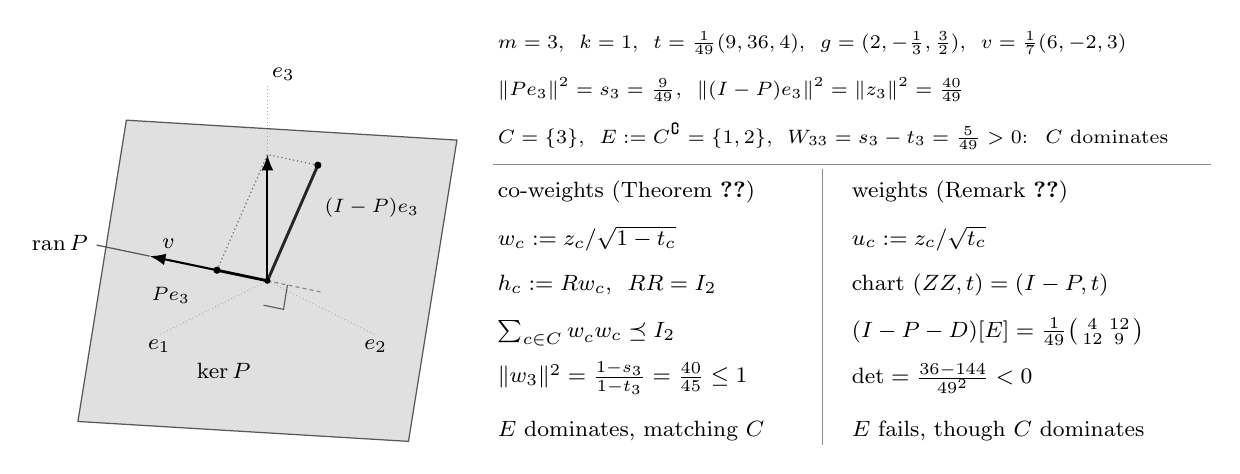
\begin{tikzpicture}[
  x=1.85cm, y=1.85cm,
  vec/.style   ={-{Latex[length=2mm,width=1.5mm]}, line width=0.75pt},
  proj/.style  ={line width=1.05pt, black!85},
  edge/.style  ={line width=0.45pt, black!65},
  hidden/.style={line width=0.45pt, black!45, dashed, dash pattern=on 1.4pt off 1.2pt},
  frame/.style ={densely dotted, line width=0.3pt, black!35},
  constr/.style={densely dotted, line width=0.45pt, black!55},
  hair/.style  ={line width=0.4pt, black!45},
  every node/.style={inner sep=1.5pt, font=\small}]

% ---- the kernel plane, as a rectangle through the origin -----------------
\coordinate (Cpp) at ( 1.3009, 0.9659);   %  2.00 d1 + 1.05 d2
\coordinate (Cpm) at ( 0.9683,-1.1025);   %  2.00 d1 - 1.05 d2
\coordinate (Cmm) at (-1.3009,-0.9659);   % -2.00 d1 - 1.05 d2
\coordinate (Cmp) at (-0.9683, 1.1025);   % -2.00 d1 + 1.05 d2
\path[fill=black!12] (Cpp)--(Cmp)--(Cmm)--(Cpm)--cycle;
\draw[edge]          (Cpp)--(Cmp)--(Cmm)--(Cpm)--cycle;

% ---- the three coordinate axes, as a frame of reference ------------------
\coordinate (O)  at (0,0);
\coordinate (A1) at (-0.7425,-0.3712);    % 1.05 e_1
\coordinate (A2) at ( 0.7425,-0.3712);    % 1.05 e_2
\coordinate (A3) at ( 0,      1.3423);    % 1.55 e_3
\draw[frame] (O)--(A1);
\draw[frame] (O)--(A2);
\draw[frame] (O)--(A3);
\node[anchor=north,      font=\footnotesize] at (A1) {$e_1$};
\node[anchor=north,      font=\footnotesize] at (A2) {$e_2$};
\node[anchor=south west, font=\footnotesize] at (A3) {$e_3$};

% ---- the range of the chart: the line R v --------------------------------
\coordinate (V)    at (-0.8081, 0.1691);  % v      = ( 6,-2, 3)/7
\coordinate (Vfar) at (-1.1718, 0.2452);  % 1.45 v
\coordinate (Vneg) at ( 0.3637,-0.0761);  % -0.45 v, behind the plane
\draw[hidden] (O)--(Vneg);
\draw[edge]   (V)--(Vfar);
% the line meets the plane at a right angle: the square on -0.17v and -0.17d2
\draw[edge, line width=0.4pt]
      ( 0.1374,-0.0288)--( 0.1105,-0.1962)--(-0.0269,-0.1674);

% ---- the two shadows of e_3, and the parallelogram they close ------------
\coordinate (Pe) at (-0.3463, 0.0725);    % P e_3    = ( 18,-6, 9)/49
\coordinate (Qe) at ( 0.3463, 0.7935);    % (I-P)e_3 = (-18, 6,40)/49
\coordinate (E3) at ( 0,      0.8660);    % e_3
\draw[constr] (Pe)--(E3) (Qe)--(E3);
\draw[proj]   (O)--(Pe);
\draw[proj]   (O)--(Qe);
\fill (Pe) circle (1.3pt);
\fill (Qe) circle (1.3pt);

% ---- the unit vector on the line, and the selected basis vector ----------
\draw[vec] (O)--(V);
\draw[vec] (O)--(E3);
\fill (O) circle (1.1pt);

\node[anchor=east,       font=\footnotesize] at (-1.20, 0.26) {$\operatorname{ran}P$};
\node[anchor=south,      font=\footnotesize] at (-0.68, 0.19) {$v$};
\node[anchor=east,       font=\scriptsize]   at (-0.50,-0.10) {$Pe_3$};
\node[anchor=north west, font=\scriptsize]   at ( 0.36, 0.60) {$(I-P)e_3$};
\node[font=\footnotesize] at (-0.30,-0.62) {$\ker P$};

% ======================= the forced normalization =========================
% Nine rows 0.32 apart, the two columns starting at 1.55 and 3.98.
\begin{scope}[every node/.style={anchor=west, inner sep=1.5pt,
                                 font=\footnotesize}]
\node[font=\scriptsize] at (1.55, 1.63)
  {$m=3$, \ $k=1$, \ $t=\tfrac1{49}(9,36,4)$, \ $g=(2,-\tfrac13,\tfrac32)$,
   \ $v=\tfrac17(6,-2,3)$};
\node[font=\scriptsize] at (1.55, 1.31)
  {$\lVert Pe_3\rVert^2=s_3=\tfrac9{49}$, \
   $\lVert (I-P)e_3\rVert^2=\lVert z_3\rVert^2=\tfrac{40}{49}$};
\node[font=\scriptsize] at (1.55, 0.99)
  {$C=\{3\}$, \ $E:=C^{\complement}=\{1,2\}$, \
   $W_{33}=s_3-t_3=\tfrac5{49}>0$: \ $C$ dominates};

\draw[hair] (1.55, 0.80)--(6.48, 0.80);
\draw[hair] (3.81, 0.77)--(3.81,-1.13);

\node at (1.55, 0.61) {co-weights (Theorem~\ref{thm:duality})};
\node at (3.98, 0.61) {weights (Remark~\ref{rem:naive})};
\node at (1.55, 0.29) {$w_c:=z_c/\sqrt{1-t_c}$};
\node at (3.98, 0.29) {$u_c:=z_c/\sqrt{t_c}$};
\node at (1.55,-0.03) {$h_c:=R\adj w_c$, \ $R\adj\Sdual R=I_2$};
\node at (3.98,-0.03) {chart $(ZZ\adj,t)=(I-P,t)$};
\node at (1.55,-0.35)
  {$\textstyle\sum_{c\in C}w_c^{\vphantom{\mathsf{H}}}w_c\adj\preceq I_2$};
\node at (3.98,-0.35)
  {$(I-P-D)[E]=\tfrac1{49}\begin{psmallmatrix}4&12\\12&9\end{psmallmatrix}$};
\node at (1.55,-0.67) {$\lVert w_3\rVert^2=\tfrac{1-s_3}{1-t_3}=\tfrac{40}{45}\le1$};
\node at (3.98,-0.67) {$\det=\tfrac{36-144}{49^2}<0$};
\node at (1.55,-1.03) {$E$ dominates, matching $C$};
\node at (3.98,-1.03) {$E$ fails, though $C$ dominates};
\end{scope}

\end{tikzpicture}

  \caption{Duality at $m=3$, $k=1$ (Theorem~\ref{thm:duality}).  The vector
  $v_c=\sqrt{t_c}\,g_c$ has norm one, so the chart $P=vv\adj$ projects onto a
  line of the index space and $I-P$ onto the complementary plane, where the
  shadow of $e_3$ is the kernel row $z_3$ in coordinates.  Selecting $\{3\}$
  from $P$ and deleting it from $I-P$ are one operation, and no weight enters
  it.  The weights enter the normalization.  Rescaling the kernel rows by the
  co-weights and whitening by $\Sdual$ carries the dominating singleton
  $\{3\}$ to the dominating pair $\{1,2\}$; the rescaling by the weights of
  Remark~\ref{rem:naive}, whose chart is $(I-P,t)$ itself, refuses that pair.
  Example~\ref{ex:uneven} carries the failure in the other direction at
  $m=2$.}
  \label{fig:duality}
\end{figure}

\begin{example}\label{ex:uneven}
Take $m=2$, $k=1$, $t=(\tfrac15,\tfrac45)$ and $g=(2,\tfrac12)$; the
Parseval condition holds, $\tfrac15\cdot4+\tfrac45\cdot\tfrac14=1$.  Here
$v=\bigl(2/\sqrt5,\;1/\sqrt5\bigr)$, of norm one, so
$\ker P$ is spanned by the unit vector $z=(-1/\sqrt5,\,2/\sqrt5)$, giving
$\lvert z_1\rvert^2=\tfrac15$ and $\lvert z_2\rvert^2=\tfrac45$.  The
singleton $\{1\}$ dominates, $g_1^2=4\ge1$, and $\{2\}$ does not,
$g_2^2=\tfrac14<1$.

The correct dual: $w_1^2=\tfrac{1/5}{4/5}=\tfrac14$,
$w_2^2=\tfrac{4/5}{1/5}=4$, so
$\Sdual=\tfrac15\cdot\tfrac14+\tfrac45\cdot4=\tfrac{13}{4}$ and
$h_c^2=w_c^2/\Sdual$, that is $h_1^2=\tfrac1{13}$ and $h_2^2=\tfrac{16}{13}$.
Parseval holds, $\tfrac15\cdot\tfrac1{13}+\tfrac45\cdot\tfrac{16}{13}=1$,
and the correspondence is exact: $\{2\}$ dominates in $\dsn^{\perp}$
because $\tfrac{16}{13}\ge1$, matching $\{1\}$ upstairs, and $\{1\}$
fails downstairs because $\tfrac1{13}<1$, matching $\{2\}$ upstairs.

The naive dual of Remark~\ref{rem:naive}: $u_1^2=\tfrac{1/5}{1/5}=1$ and
$u_2^2=\tfrac{4/5}{4/5}=1$.  Both singletons dominate, so the
correspondence fails at $C=\{2\}$, which does not dominate upstairs while
its complement does downstairs.
\end{example}

At $(4,2)$ the two cells of Corollary~\ref{cor:dualcell} coincide and the
correspondence becomes an involution on the six pairs.

\begin{example}\label{ex:dualworked}
Take the design of Example~\ref{ex:chartworked}, at $(4,2)$ with
$t=\tfrac19(2,3,3,1)$ and the chart printed there.  Since $m-k=k=2$, the
dual $\dsn^{\perp}$ is again a design at $(4,2)$ and
$C\mapsto C^{\complement}$ sends pairs to pairs.

The kernel of $P$ is orthogonal to the two columns $(2,2,1,0)$ and
$(0,1,-2,2)$ of $3V$.  The integer vectors
\[
  n_1=(-5,4,2,0),\qquad n_2=(0,-2,4,5)
\]
annihilate both: $2(-5)+2(4)+1(2)=0$ and $1(4)+(-2)(2)=0$ for $n_1$,
$2(-2)+1(4)=0$ and $1(-2)+(-2)(4)+2(5)=0$ for $n_2$.  They also satisfy
$\lVert n_1\rVert^2=\lVert n_2\rVert^2=45$ and $\langle n_1,n_2\rangle=0$,
so $Z:=\tfrac1{3\sqrt5}(n_1\ n_2)$ has $Z\adj Z=I_2$ and
$ZZ\adj=I_4-P$.  Its rows are
\[
  z_0=\tfrac1{3\sqrt5}(-5,0),\quad
  z_1=\tfrac1{3\sqrt5}(4,-2),\quad
  z_2=\tfrac1{3\sqrt5}(2,4),\quad
  z_3=\tfrac1{3\sqrt5}(0,5),
\]
of squared lengths $\tfrac19(5,4,4,5)$, which is $1-s_c$ index by index.

Rescale by the co-weights $1-t=\tfrac19(7,6,6,8)$.  Then
$\lVert w_c\rVert^2=\bigl(\tfrac57,\tfrac23,\tfrac23,\tfrac58\bigr)$ and
the operator \eqref{eq:dualgram} is
\[
  \Sdual=\sum_c t_c\,w_c^{\vphantom{\mathsf{H}}}w_c\adj
    =\diag\bigl(\tfrac8{21},\tfrac7{24}\bigr),
  \qquad \det\Sdual=\tfrac19,
\]
positive definite as Lemma~\ref{lem:dualgram} requires.  Take
$R=\diag\bigl(\sqrt{21/8},\sqrt{24/7}\bigr)$, so that $R\adj\Sdual R=I_2$
as in Lemma~\ref{lem:whiten}.  The dual atoms $h_c=R\adj w_c$ are
\[
  h_0=\tfrac14(-\sqrt{30},0),\quad
  h_1=\tfrac1{\sqrt{35}}(7,-4),\quad
  h_2=\tfrac1{2\sqrt{35}}(7,16),\quad
  h_3=\tfrac17(0,\sqrt{105}),
\]
and the radicals cancel again in the rank-one terms:
\[
  h_0^{\vphantom{\mathsf{H}}}h_0\adj
    =\begin{pmatrix}\tfrac{15}8&0\\[2pt]0&0\end{pmatrix},
  \quad
  h_1^{\vphantom{\mathsf{H}}}h_1\adj
    =\begin{pmatrix}\tfrac75&-\tfrac45\\[2pt]
                    -\tfrac45&\tfrac{16}{35}\end{pmatrix},
  \quad
  h_2^{\vphantom{\mathsf{H}}}h_2\adj
    =\begin{pmatrix}\tfrac7{20}&\tfrac45\\[2pt]
                    \tfrac45&\tfrac{64}{35}\end{pmatrix},
  \quad
  h_3^{\vphantom{\mathsf{H}}}h_3\adj
    =\begin{pmatrix}0&0\\[2pt]0&\tfrac{15}7\end{pmatrix}.
\]
Their $t$-weighted sum is $I_2$: the first diagonal entries give
$\tfrac5{12}+\tfrac7{15}+\tfrac7{60}=1$, the two off-diagonal
contributions cancel, and the second diagonal entries give
$\tfrac{16}{105}+\tfrac{64}{105}+\tfrac{25}{105}=1$.  So $\dsn^{\perp}$ is
a design at $(4,2)$ carrying the weights of $\dsn$, with leverage scores
$t_c\lVert h_c\rVert^2=\tfrac1{84}(35,52,61,20)$ summing to $2$.

Figure~\ref{fig:dualworked} runs the correspondence at all six pairs.  Take
two of them.  Upstairs $\{0,2\}$ dominates with slack
zero; downstairs its complement gives
\[
  h_1^{\vphantom{\mathsf{H}}}h_1\adj+h_3^{\vphantom{\mathsf{H}}}h_3\adj-I_2
   =\begin{pmatrix}\tfrac25&-\tfrac45\\[3pt]
                   -\tfrac45&\tfrac85\end{pmatrix},
\]
of determinant $0$ and trace $2$, so $\{1,3\}$ dominates in $\dsn^{\perp}$
with slack zero as well.  The spectra are $\{1,\tfrac83\}$ upstairs and
$\{1,3\}$ downstairs, and $\lmin=1$ at both ends.  Upstairs $\{2,3\}$
fails; downstairs
$h_0^{\vphantom{\mathsf{H}}}h_0\adj+h_1^{\vphantom{\mathsf{H}}}h_1\adj-I_2$
has $(2,2)$ entry $\tfrac{16}{35}-1<0$, so $\{0,1\}$ fails in
$\dsn^{\perp}$.

The naive dual of Remark~\ref{rem:naive} is also a design at $(4,2)$ with
the weights of $\dsn$, of chart $(I_4-P,t)$ and gap
\[
  (I_4-P)-D=\tfrac19\begin{pmatrix}
    3&-4&-2&0\\ -4&1&0&-2\\ -2&0&1&4\\ 0&-2&4&4\end{pmatrix} .
\]
Over $\{0,1\},\{0,2\},\{0,3\},\{1,2\},\{1,3\},\{2,3\}$ its six principal
$2\times2$ minors, multiplied by $81$, are $-13$, $-1$, $12$, $1$, $0$,
$-12$.  Five carry the sign the correspondence demands.  The sixth is
$E=\{0,2\}$, whose block
$\tfrac19\begin{psmallmatrix}3&-2\\-2&1\end{psmallmatrix}$ has
determinant $-\tfrac1{81}$, so $E$ fails there, while the complementary
pair $\{1,3\}$ dominates strictly in $\dsn$ with $81\det W[\{1,3\}]=2$.
\end{example}

\begin{figure}[ht]
  \centering
  % Duality at (m,k) = (4,2), the self-dual cell, on the design of
% Example ex:chartworked.  Three panels: the kernel rows z_c, the dual atoms
% h_c against the unit circle, and the two normalizations run against each
% other over all six pairs.  The cell is self-dual, m - k = k = 2, so the dual
% design lives at (4,2) as well and the complement map C -> C^c is an
% involution on the six pairs: the opposite-edge map of the square in
% figures/chartworked.tex.
%
% PROJECTION.  Both drawn panels are plane figures and carry no projection of a
% higher-dimensional space; the map is the identity of R^2, scaled by 1.55cm in
% the kernel panel and by 1.05cm in the dual-atom panel,
%   panel A:  X = 1.55 x_1,  Y = 1.55 x_2
%   panel B:  X = 1.05 x_1,  Y = 1.05 x_2
% so no viewing normal and no visibility rule are needed and no line is hidden.
% The two scales differ because the longest kernel row has norm
% sqrt(5/9) = 0.7453560 while the longest dual atom has norm
% sqrt(61/28) = 1.4759985, a ratio of sqrt(549/140) = 1.9802597; at a common
% scale one panel would be twice the other.  The unit circle is drawn in both,
% so the eye compares against it and not across panels.
%
% THE PRIMAL DATA.  Over R, m = 4, k = 2, t = (2,3,3,1)/9,
%   g_0 = (sqrt2,0), g_1 = (2,1)/sqrt3, g_2 = (1,-2)/sqrt3, g_3 = (0,2),
% with s = (4,5,5,4)/9 and the rational chart 9P = [[4,4,2,0],[4,5,0,2],
% [2,0,5,-4],[0,2,-4,4]].  See figures/chartworked.tex for the Parseval check.
%
% THE KERNEL BASIS.  ker P is orthogonal to the two columns (2,2,1,0) and
% (0,1,-2,2) of 3V.  The integer vectors n1 = (-5,4,2,0) and n2 = (0,-2,4,5)
% annihilate both -- 2(-5)+2(4)+1(2) = 0, 1(4)+(-2)(2) = 0, 2(-2)+1(4) = 0,
% 1(-2)+(-2)(4)+2(5) = 0 -- and satisfy n1.n1 = n2.n2 = 45, n1.n2 = 0.  So
% Z = [n1 n2]/(3 sqrt5) has Z^T Z = I_2 and Z Z^T = I - P, and its rows are
%   z_0 = (-5, 0)/(3 sqrt5)   |z_0|^2 = 5/9 = 1 - s_0
%   z_1 = ( 4,-2)/(3 sqrt5)   |z_1|^2 = 4/9 = 1 - s_1
%   z_2 = ( 2, 4)/(3 sqrt5)   |z_2|^2 = 4/9 = 1 - s_2
%   z_3 = ( 0, 5)/(3 sqrt5)   |z_3|^2 = 5/9 = 1 - s_3
% Panel A draws these four rows.
%
% THE TWO NORMALIZATIONS.  With 1 - t = (7,6,6,8)/9,
%   w_c = z_c/sqrt(1-t_c):  |w_c|^2 = (5/7, 2/3, 2/3, 5/8),
%   S^perp = sum_c t_c w_c w_c^T = diag(8/21, 7/24),  det = 1/9,
%   R = diag(sqrt(21/8), sqrt(24/7)),  R^T S^perp R = I_2,
%   h_0 = (-sqrt(30)/4, 0)          = (-sqrt30, 0)/4       |h_0|^2 = 15/8
%   h_1 = ( sqrt(35)/5, -4 sqrt(35)/35) = (7,-4)/sqrt35     |h_1|^2 = 13/7
%   h_2 = ( sqrt(35)/10, 8 sqrt(35)/35) = (7,16)/(2 sqrt35) |h_2|^2 = 61/28
%   h_3 = ( 0, sqrt(105)/7)         = (0, sqrt105)/7        |h_3|^2 = 15/7
% and sum_c t_c |h_c|^2 = 5/12 + 13/21 + 61/84 + 5/21 = 2 = m - k.  The naive
% rescaling u_c = z_c/sqrt(t_c) gives |u_c|^2 = (5/2, 4/3, 4/3, 5) and chart
% (Z Z^T, t) = (I - P, t), whose gap is 9(I-P-D) = [[3,-4,-2,0],[-4,1,0,-2],
% [-2,0,1,4],[0,-2,4,4]].  Panel B draws the h_c; the u_c are not drawn, since
% u_c is a positive multiple of z_c and panel A already carries their
% directions, all four of which the naive dual keeps.
%
% ELLIPSE FRAME.  At E = {1,3} the dual selection matrix is
% h_1 h_1^T + h_3 h_3^T = [[7/5,-4/5],[-4/5,13/5]], of spectrum {1,3}, so the
% ellipse {x : x^T (h_1 h_1^T + h_3 h_3^T) x = 1} has semi-axes 1 and
% 1/sqrt3 = 0.5773503, the long one along the eigenvector (2,1)/sqrt5 at
% atan2(1,2) = 26.5651 degrees, and it touches the unit circle exactly at
% +-(2,1)/sqrt5 = +-(0.8944272, 0.4472136).  Upstairs the same picture stands
% at C = {0,2} with spectrum {1, 8/3} and tangency along (1,2)/sqrt5.
%
% THE TABLE.  81 det W[C] over {0,1}, {0,2}, {0,3}, {1,2}, {1,3}, {2,3} is
% -12, 0, +6, +4, +2, -10; det(sum_{c in E} h_c h_c^T - I_2) over the
% complementary pairs {2,3}, {1,3}, {1,2}, {0,3}, {0,2}, {0,1} is -18/7, 0,
% 27/28, 1, 3/8, -15/8; and 81 det (I-P-D)[E] over the same is -12, 0, +1, +12,
% -1, -13.  The sign agrees in all six rows for the co-weight normalization and
% in five for the weight normalization, the exception being C = {1,3} against
% E = {0,2}, boxed in the body.
%
% DISCLOSED: this design is new to the paper and no Lean declaration mentions
% it; every number here was computed in exact arithmetic outside the assistant
% -- rational for the chart, S^perp, the leverage scores and all three minor
% columns, algebraic for z_c, R, h_c and the ellipse frame, whose decimals in
% the body are truncations of those exact values.  Theorem thm:duality is
% mechanized over R, but as an EXISTENTIAL over dual designs, and by a
% construction that is not the one drawn: the formal proof whitens the
% co-Parseval operator and takes the dual atoms from an orthonormal
% completion.  What panel B draws is therefore the printed
% construction, and the formal statement covers it only in asserting that some
% dual design with these weights flips domination.  No complex Naimark duality
% exists in the development, so nothing here transfers to C.
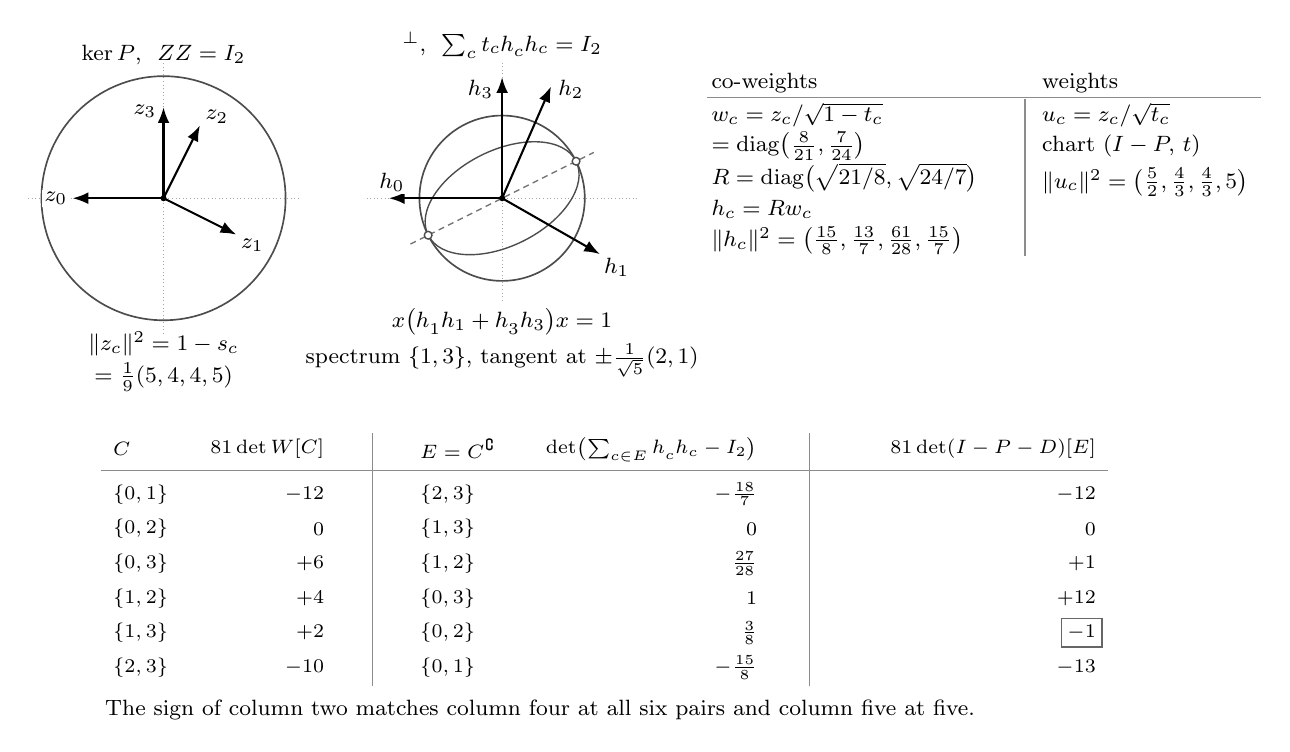
\begin{tikzpicture}[
  x=1cm, y=1cm,
  vec/.style   ={-{Latex[length=2mm,width=1.5mm]}, line width=0.75pt},
  rim/.style   ={line width=0.6pt, black!70},
  lev/.style   ={line width=0.5pt, black!70},
  frame/.style ={densely dotted, line width=0.3pt, black!35},
  tight/.style ={line width=0.5pt, black!55, dashed,
                 dash pattern=on 2.2pt off 1.6pt},
  hair/.style  ={line width=0.4pt, black!45},
  box/.style   ={line width=0.45pt, black!60},
  tag/.style   ={font=\footnotesize, fill=white, inner sep=0.8pt},
  every node/.style={inner sep=1.5pt, font=\small}]

% ==================== panel A: the rows of the kernel basis ================
\begin{scope}[shift={(2.00,3.90)}]
  \draw[frame] (-1.72,0)--(1.72,0);
  \draw[frame] (0,-1.72)--(0,1.72);
  \draw[rim] (0,0) circle (1.55);

  \draw[vec] (0,0)--(-1.15530, 0.00000);   % z_0 = (-5, 0)/(3 sqrt5)
  \draw[vec] (0,0)--( 0.92424,-0.46212);   % z_1 = ( 4,-2)/(3 sqrt5)
  \draw[vec] (0,0)--( 0.46212, 0.92424);   % z_2 = ( 2, 4)/(3 sqrt5)
  \draw[vec] (0,0)--( 0.00000, 1.15530);   % z_3 = ( 0, 5)/(3 sqrt5)
  \fill (0,0) circle (1.1pt);
  \node[tag, anchor=east]       at (-1.19, 0.00) {$z_0$};
  \node[tag, anchor=north west] at ( 0.95,-0.48) {$z_1$};
  \node[tag, anchor=south west] at ( 0.50, 0.92) {$z_2$};
  \node[tag, anchor=east]       at (-0.06, 1.10) {$z_3$};

  \node[anchor=south, font=\footnotesize] at (0,1.64)
    {$\ker P$, \ $Z\adj Z=I_2$};
  \node[anchor=north, align=center, font=\footnotesize] at (0,-1.64)
    {$\lVert z_c\rVert^2=1-s_c$\\[2pt] $=\tfrac19(5,4,4,5)$};
\end{scope}

% ==================== panel B: the dual atoms h_c ==========================
\begin{scope}[shift={(6.30,3.90)}]
  \draw[frame] (-1.72,0)--(1.72,0);
  \draw[frame] (0,-1.30)--(0,1.72);
  \draw[rim] (0,0) circle (1.05);
  % the ellipse of h_1 h_1^H + h_3 h_3^H, spectrum {1,3}: semi-axes 1 and
  % 1/sqrt3, the long one along (2,1)/sqrt5
  \draw[lev, rotate=26.5651] (0,0) ellipse (1.05 and 0.60622);
  \draw[tight] (-1.16454,-0.58227)--(1.16454,0.58227);       % +-1.24 (2,1)/sqrt5
  \draw[lev, fill=white] ( 0.93915, 0.46957) circle (1.4pt); % + (2,1)/sqrt5
  \draw[lev, fill=white] (-0.93915,-0.46957) circle (1.4pt); % - (2,1)/sqrt5

  \draw[vec] (0,0)--(-1.43777, 0.00000);   % h_0 = (-sqrt30/4, 0)
  \draw[vec] (0,0)--( 1.24238,-0.70993);   % h_1 = (sqrt35/5, -4 sqrt35/35)
  \draw[vec] (0,0)--( 0.62119, 1.41986);   % h_2 = (sqrt35/10, 8 sqrt35/35)
  \draw[vec] (0,0)--( 0.00000, 1.53704);   % h_3 = (0, sqrt105/7)
  \fill (0,0) circle (1.1pt);
  \node[tag, anchor=south]      at (-1.40, 0.05) {$h_0$};
  \node[tag, anchor=north west] at ( 1.26,-0.72) {$h_1$};
  \node[tag, anchor=west]       at ( 0.68, 1.38) {$h_2$};
  \node[tag, anchor=east]       at (-0.08, 1.38) {$h_3$};

  \node[anchor=south, font=\footnotesize] at (0,1.72)
    {$\dsn^{\perp}$, \
     $\textstyle\sum_ct_ch_c^{\vphantom{\mathsf{H}}}h_c\adj=I_2$};
  \node[anchor=north, align=center, font=\footnotesize] at (0,-1.34)
    {$x\adj\bigl(h_1^{\vphantom{\mathsf{H}}}h_1\adj
       +h_3^{\vphantom{\mathsf{H}}}h_3\adj\bigr)x=1$\\[2pt]
     spectrum $\{1,3\}$, tangent at $\pm\tfrac1{\sqrt5}(2,1)$};
\end{scope}

% =============== the two normalizations, side by side ======================
\begin{scope}[every node/.style={anchor=west, inner sep=1.5pt,
                                 font=\footnotesize}]
  \node at ( 8.90, 5.36) {co-weights};
  \node at (13.10, 5.36) {weights};
  % the header rule spans the block it underlines: from the west edge of the
  % left column's nodes at 8.90 to the east edge of the widest ink in the right
  % column, the 79.25pt of the u_c-norm row at 13.10 plus its 1.5pt inner sep,
  % which is 15.938; its node box reaches 15.991, so the rule adds no width.
  \draw[hair] ( 8.90, 5.18)--(15.94, 5.18);
  \draw[hair] (12.94, 5.16)--(12.94, 3.16);
  \node at ( 8.90, 4.96) {$w_c=z_c/\sqrt{1-t_c}$};
  \node at (13.10, 4.96) {$u_c=z_c/\sqrt{t_c}$};
  \node at ( 8.90, 4.56) {$\Sdual=\diag\bigl(\tfrac8{21},\tfrac7{24}\bigr)$};
  \node at (13.10, 4.56) {chart $(I-P,\,t)$};
  \node at ( 8.90, 4.16) {$R=\diag\bigl(\sqrt{21/8},\sqrt{24/7}\bigr)$};
  \node at (13.10, 4.10)
    {$\lVert u_c\rVert^2=\bigl(\tfrac52,\tfrac43,\tfrac43,5\bigr)$};
  \node at ( 8.90, 3.76) {$h_c=R\adj w_c$};
  \node at ( 8.90, 3.36)
    {$\lVert h_c\rVert^2=\bigl(\tfrac{15}8,\tfrac{13}7,
       \tfrac{61}{28},\tfrac{15}7\bigr)$};
\end{scope}

% ==================== the six pairs, three columns =========================
\begin{scope}[every node/.style={inner sep=1.5pt, font=\scriptsize}]
  \node[anchor=west] at ( 1.30, 0.72) {$C$};
  \node[anchor=east] at ( 4.10, 0.72) {$81\det W[C]$};
  \node[anchor=west] at ( 5.20, 0.72) {$E=C^{\complement}$};
  \node[anchor=east] at ( 9.60, 0.72)
    {$\det\bigl(\sum_{c\in E}h_c^{\vphantom{\mathsf{H}}}h_c\adj-I_2\bigr)$};
  \node[anchor=east] at (13.90, 0.72) {$81\det(I-P-D)[E]$};
  \draw[hair] ( 1.20, 0.44)--(14.00, 0.44);
  \draw[hair] ( 4.65, 0.92)--( 4.65,-2.30);
  \draw[hair] (10.20, 0.92)--(10.20,-2.30);

  % Rows 0.44 apart, in the order {0,1} {0,2} {0,3} {1,2} {1,3} {2,3}.  The
  % pitch is set by column four: a \tfrac at \scriptsize has height 7.137pt and
  % depth 3.137pt, so a pitch of 10.274pt = 0.3610 would put the denominator of
  % one fraction row on the numerator of the next, which 0.36 did; 0.44 =
  % 12.520pt leaves 2.25pt, the gap the reading block of
  % figures/chartworked.tex runs at.  The header sits at 0.72 rather than 0.66
  % so that its tallest entry, whose centred box reaches 6.014pt below the row,
  % clears the rule at 0.44 by 1.94pt instead of 0.24pt.
  \foreach \yy/\CC/\dW/\EE/\dH/\dN in {%
     0.14/{\{0,1\}}/{-12}/{\{2,3\}}/{-\tfrac{18}7}/{-12},
    -0.30/{\{0,2\}}/{0}/{\{1,3\}}/{0}/{0},
    -0.74/{\{0,3\}}/{+6}/{\{1,2\}}/{\tfrac{27}{28}}/{+1},
    -1.18/{\{1,2\}}/{+4}/{\{0,3\}}/{1}/{+12},
    -1.62/{\{1,3\}}/{+2}/{\{0,2\}}/{\tfrac38}/{-1},
    -2.06/{\{2,3\}}/{-10}/{\{0,1\}}/{-\tfrac{15}8}/{-13}}{%
    \node[anchor=west] at ( 1.30,\yy) {$\CC$};
    \node[anchor=east] at ( 4.10,\yy) {$\dW$};
    \node[anchor=west] at ( 5.20,\yy) {$\EE$};
    \node[anchor=east] at ( 9.60,\yy) {$\dH$};
    \node[anchor=east] at (13.90,\yy) {$\dN$};}
  % The one row where the weight normalization disagrees in sign.  The entry
  % $-1$ is 10.861pt wide with 1.5pt of inner sep, so its ink runs from 13.4658
  % to 13.8473 and, centred on the row, from 0.1052 above to 0.1052 below it;
  % the frame clears that by 1.87, 2.07 and 2.13pt on the left, the right and
  % the two horizontals.  The previous frame cleared the left by 0.26pt.
  \draw[box] (13.40,-1.80) rectangle (13.92,-1.44);

  \node[anchor=west, font=\footnotesize] at ( 1.20,-2.60)
    {The sign of column two matches column four at all six pairs and
     column five at five.};
\end{scope}

\end{tikzpicture}

  \caption{Duality at $(4,2)$, where the dual cell is the cell itself, on
  the design of Example~\ref{ex:chartworked}.  Left: the rows of an
  orthonormal basis of $\ker P$, of squared lengths
  $1-s_c=\tfrac19(5,4,4,5)$.  Centre: the dual atoms of
  Theorem~\ref{thm:duality}, and the ellipse of
  $h_1^{\vphantom{\mathsf{H}}}h_1\adj+h_3^{\vphantom{\mathsf{H}}}h_3\adj$,
  of spectrum $\{1,3\}$, touching the unit circle at
  $\pm\tfrac1{\sqrt5}(2,1)$.  Right: the two normalizations of
  Remark~\ref{rem:naive}.  Below: at each of the six pairs, the gap minor of
  $\dsn$ and the minor of each normalization, the boxed entry the one at which
  the rescaling by the weights takes the wrong sign.
  The dual atoms drawn are those of the construction above
  Theorem~\ref{thm:duality}; the mechanized statement asserts only that some
  dual design with these weights flips domination.}
  \label{fig:dualworked}
\end{figure}

\subsection{Corank one}\label{sec:corankone}

Let $m=k+1$ with $k\ge1$.  Then $\ker P$ is a line, spanned by a unit
vector $z\in\FF^{m}$, and $P=I-zz\adj$.  Set
\begin{equation}\label{eq:pvars}
  p_c\;:=\;\frac{\lvert z_c\rvert^2}{1-t_c}
  \;=\;\frac{1-t_c\ell_c}{1-t_c},
\end{equation}
the second expression by $\lvert z_c\rvert^2=1-P_{cc}=1-s_c$
(Proposition~\ref{prop:chartid}).  Since $z$ is a unit vector,
\begin{equation}\label{eq:pnorm}
  \sum_c p_c\,(1-t_c)\;=\;\sum_c\lvert z_c\rvert^2\;=\;1,
  \qquad\text{while}\qquad
  \sum_c (1-t_c)\;=\;m-1\;=\;k .
\end{equation}
The $p_c$ therefore have co-weighted mean $1/k$.  Domination compares a
positive diagonal with a rank-one perturbation of it, and one scalar
decides such a comparison.  Figure~\ref{fig:rankoneball} draws the
comparison.

\begin{lemma}[Lean]\label{lem:rankone}
Let $A\pd0$ and let $b$ be a vector, and put $q:=b\adj A^{-1}b$.  Then
\[
  A-bb\adj\psd0\iff q\le1,
  \qquad
  A-bb\adj\pd0\iff q<1 .
\]
\end{lemma}

\begin{proof}
Put $y:=A^{-1}b$, so that $Ay=b$ and
$q=\langle y,b\rangle=\langle y,Ay\rangle$: the number $q$ is the squared
length of $y$ in the inner product $\langle\cdot,A\cdot\rangle$, and in
particular $q\ge0$.  The form of the perturbed matrix is
$\langle x,(A-bb\adj)x\rangle=\langle x,Ax\rangle-\lvert\langle
b,x\rangle\rvert^2$.

Suppose $q\le1$.  The form $\langle\cdot,A\cdot\rangle$ is an inner
product, and $\langle b,x\rangle=\langle Ay,x\rangle=\langle y,Ax\rangle$
is the $A$-inner product of $y$ and $x$; Cauchy--Schwarz in it gives
$\lvert\langle b,x\rangle\rvert^2\le q\,\langle x,Ax\rangle$.  Hence
$\langle x,(A-bb\adj)x\rangle\ge(1-q)\langle x,Ax\rangle$, which is
nonnegative, and strictly positive for $x\ne0$ when $q<1$.

Conversely, evaluate at $x=y$: the form equals $q-q^2=q(1-q)$.  If
$A-bb\adj\psd0$ this is nonnegative, which forces $q\le1$ since $q\ge0$.
If moreover $q=1$ then $y\ne0$, because $\langle y,Ay\rangle=1$, and the
form vanishes at $y$, so $A-bb\adj$ is not positive definite.
\end{proof}

\begin{figure}[ht]
  \centering
  % The rank-one criterion as a point-in-ellipsoid test, drawn at three
% coordinates.  A = diag(4, 9/4, 1) is positive definite, so the locus q = 1 is
% the ellipsoid with semi-axes 2, 3/2, 1, and three vectors b run from the
% origin: (1, 3/4, 0) with q = 1/2, (1, 0, sqrt3/2) with q = 1, (0, 3/2, 1) with
% q = 2.  Each of the three lies in a coordinate plane, so the point where its
% ray meets the ellipsoid -- the open circle, at 1/sqrt(q) times b -- sits on a
% drawn principal ellipse.  Orthographic projection of R^3 with azimuth 20 and
% elevation 22 degrees, scaled by 2.20cm:
%   X = 2.20(-0.342020 x_1 + 0.939693 x_2)
%   Y = 2.20(-0.352015 x_1 - 0.128123 x_2 + 0.927184 x_3)
% Every coordinate below is the parenthesised value, with its source triple in a
% trailing comment; the 2.20cm is carried by the x and y unit vectors.  A curve
% is given by the projections of two conjugate semi-axis vectors, so that
% (X, Y) = (cos u) proj(first) + (sin u) proj(second).
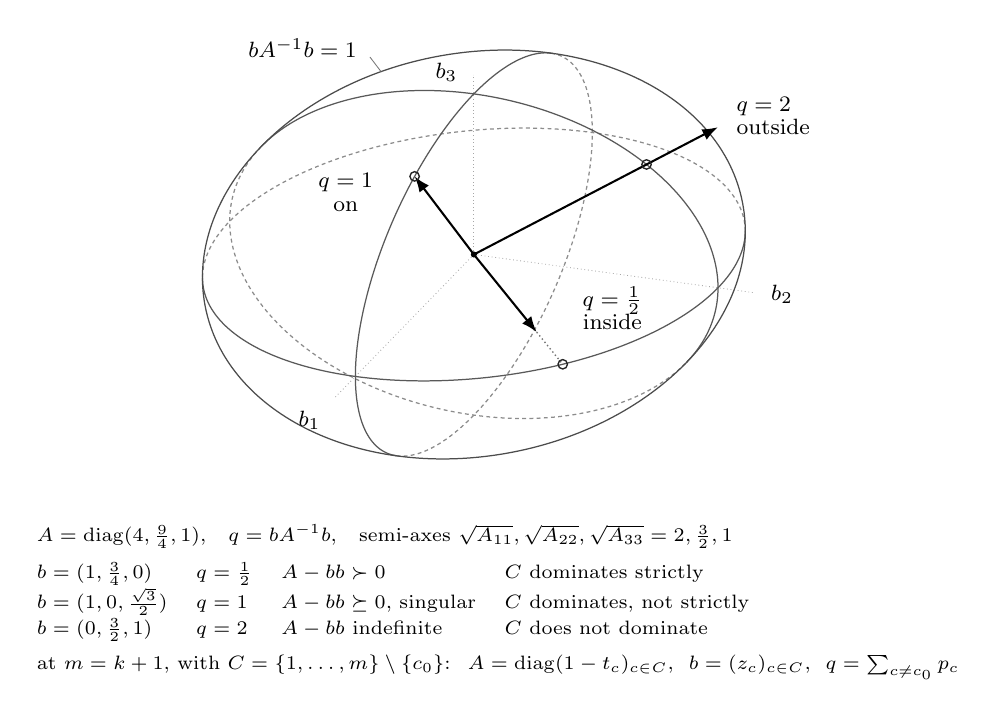
\begin{tikzpicture}[
  x=2.20cm, y=2.20cm,
  vec/.style={-{Latex[length=2mm,width=1.5mm]}, line width=0.75pt},
  frame/.style={densely dotted, line width=0.3pt, black!35},
  edge/.style={line width=0.45pt, black!65},
  rim/.style={line width=0.45pt, black!70},
  hidden/.style={line width=0.45pt, black!45, dashed, dash pattern=on 1.4pt off 1.2pt},
  slack/.style={densely dotted, line width=0.5pt, black!55},
  hit/.style={line width=0.5pt, black!85},
  lead/.style={line width=0.3pt, black!55},
  every node/.style={font=\small}]

% ---- the three coordinate axes, as a frame of reference ------------------
% each runs from the origin past its pole, which sits on the ellipsoid
\draw[frame] (0,0) -- (-0.807167,-0.830755);   % (2.36, 0,     0    )
\draw[frame] (0,0) -- ( 1.620970,-0.221012);   % (0,    1.725, 0    )
\draw[frame] (0,0) -- ( 0,        1.038446);   % (0,    0,     1.12 )

% ---- the ellipsoid: three principal ellipses, hidden arcs first ----------
% A point x of the ellipsoid faces the viewer when (A^{-1}d).x > 0, with
% d = (0.871268, 0.317116, 0.374607) the viewing direction; that inequality
% cuts each principal ellipse at the two parameters recorded below.
% E_12, semi-axis vectors (2,0,0) -> (-0.684040,-0.704030)
%                     and (0,3/2,0) -> ( 1.409539,-0.192185)
\draw[hidden, variable=\u, domain=115.887:295.887, samples=61, smooth]
  plot ({-0.684040*cos(\u)+1.409539*sin(\u)}, {-0.704030*cos(\u)-0.192185*sin(\u)});
% E_13, semi-axis vectors (2,0,0) and (0,0,1) -> (0, 0.927184)
\draw[hidden, variable=\u, domain=130.693:310.693, samples=61, smooth]
  plot ({-0.684040*cos(\u)}, {-0.704030*cos(\u)+0.927184*sin(\u)});
% E_23, semi-axis vectors (0,3/2,0) and (0,0,1)
\draw[hidden, variable=\u, domain=150.562:330.562, samples=61, smooth]
  plot ({1.409539*cos(\u)}, {-0.192185*cos(\u)+0.927184*sin(\u)});
\draw[edge, variable=\u, domain=-64.113:115.887, samples=61, smooth]
  plot ({-0.684040*cos(\u)+1.409539*sin(\u)}, {-0.704030*cos(\u)-0.192185*sin(\u)});
\draw[edge, variable=\u, domain=-49.307:130.693, samples=61, smooth]
  plot ({-0.684040*cos(\u)}, {-0.704030*cos(\u)+0.927184*sin(\u)});
\draw[edge, variable=\u, domain=-29.438:150.562, samples=61, smooth]
  plot ({1.409539*cos(\u)}, {-0.192185*cos(\u)+0.927184*sin(\u)});
% the silhouette: the contour generator is the section of the ellipsoid by the
% plane (A^{-1}d).x = 0, and its projection is the ellipse through
% (1.566752, 0.134478) and (0, 1.172254) at the two conjugate parameters,
% equivalently the ellipse of semi-axes 1.579547 and 1.162758 turned by
% 10.8171 degrees
\draw[rim, rotate=10.8171] (0,0) ellipse (1.579547 and 1.162758);

% ---- the three vectors, each with the point where its ray leaves ----------
% q = 1/2: the ray leaves at sqrt2 times b, on E_12 at parameter 45 degrees
\draw[vec]   (0,0) -- (0.362749,-0.448107);                 % b = (1, 3/4, 0)
\draw[slack] (0.362749,-0.448107) -- (0.513005,-0.633719);  % (1.414214, 1.060660, 0)
\draw[hit]   (0.513005,-0.633719) circle (1.7pt);
% q = 1: the tip is itself the exit point, on E_13 at parameter 60 degrees
\draw[vec] (0,0) -- (-0.342020,0.450950);                   % b = (1, 0, sqrt3/2)
\draw[hit] (-0.342020,0.450950) circle (1.7pt);
% q = 2: the shaft leaves at b over sqrt2, on E_23 at parameter 45 degrees
\draw[vec] (0,0) -- (1.409539,0.734999);                    % b = (0, 3/2, 1)
\draw[hit] (0.996695,0.519723) circle (1.7pt);              % (0, 1.060660, 0.707107)
\fill (0,0) circle (1.1pt);

% ---- labels ---------------------------------------------------------------
\node[anchor=north east, font=\footnotesize] at (-0.83,-0.85) {$b_1$};
\node[anchor=west,       font=\footnotesize] at ( 1.66,-0.23) {$b_2$};
\node[anchor=east,       font=\footnotesize] at (-0.04, 1.05) {$b_3$};
\draw[lead] (-0.60,1.140) -- (-0.536,1.056);   % to the rim at parameter 110 degrees
\node[anchor=east, align=right, font=\footnotesize] at (-0.62,1.19)
  {$b\adj A^{-1}b=1$};
\node[align=center, font=\footnotesize] at ( 0.80,-0.31) {$q=\tfrac12$\\[-1pt] inside};
\node[align=center, font=\footnotesize] at (-0.74, 0.36) {$q=1$\\[-1pt] on};
\node[anchor=west, align=left, font=\footnotesize] at ( 1.46, 0.80)
  {$q=2$\\[-1pt] outside};

% ---- the reading, below the picture ---------------------------------------
\node[anchor=north, align=left, font=\scriptsize] at (0.14,-1.50) {%
  $A=\diag(4,\tfrac94,1)$,\quad $q=b\adj A^{-1}b$,\quad
  semi-axes $\sqrt{A_{11}},\sqrt{A_{22}},\sqrt{A_{33}}=2,\tfrac32,1$\\[4pt]
  \begin{tabular}{@{}l@{\hspace{1.3em}}l@{\hspace{1.3em}}l@{\hspace{1.3em}}l@{}}
    $b=(1,\tfrac34,0)$          & $q=\tfrac12$ & $A-bb\adj\pd0$
      & $C$ dominates strictly\\[1pt]
    $b=(1,0,\tfrac{\sqrt3}{2})$ & $q=1$        & $A-bb\adj\psd0$, singular
      & $C$ dominates, not strictly\\[1pt]
    $b=(0,\tfrac32,1)$          & $q=2$        & $A-bb\adj$ indefinite
      & $C$ does not dominate\\
  \end{tabular}\\[4pt]
  at $m=k+1$, with $C=\{1,\dots,m\}\setminus\{c_0\}$: \
  $A=\diag(1-t_c)_{c\in C}$, \ $b=(z_c)_{c\in C}$, \ $q=\sum_{c\ne c_0}p_c$};

\end{tikzpicture}

  \caption{Lemma~\ref{lem:rankone} in three coordinates.  The locus $q=1$ is the
  image of the unit sphere under $A^{1/2}$, and the criterion asks which side of
  it $b$ lies on; the open circle marks where the ray through $b$ leaves the
  ellipsoid.  At $m=k+1$ the comparison is \eqref{eq:corankone}, the ratio at the
  omitted index against the $t$-weighted mean of all of them.  The ellipsoid then
  lives in the index space: its coordinates are the selected indices, its
  semi-axes are the square roots of the co-weights $1-t_c$, and the vectors $g_c$
  do not enter.  Figure~\ref{fig:jensen} is the same comparison in bar-chart
  form.}
  \label{fig:rankoneball}
\end{figure}

\begin{theorem}[Lean]\label{thm:corankone}
Let $m=k+1$, $k\ge1$, over either field.
\begin{enumerate}
\item[(i)] The complement of $\{c_0\}$ dominates if and only if
\begin{equation}\label{eq:corankone}
  p_{c_0}\;\ge\;\sum_{c} t_c\,p_c ,
\end{equation}
and it dominates strictly if and only if the inequality is strict.
\item[(ii)] $\Gtz(k+1,k)$ and $\GtzC(k+1,k)$ hold.
\item[(iii)] Equality holds in \eqref{eq:corankone} for every $c_0$ if
and only if $p_c\equiv1/k$, if and only if
\begin{equation}\label{eq:tielaw}
  k\,t_c\,\ell_c \;=\; k-1+t_c \qquad (1\le c\le m),
\end{equation}
and in that case every $k$-subset dominates and none dominates strictly.
\item[(iv)] For every weight vector $t$ on $k+1$ atoms there is a design
with weights exactly $t$ satisfying \eqref{eq:tielaw}.
\end{enumerate}
\end{theorem}

\begin{proof}
(i) Put $C:=\{1,\dots,m\}\setminus\{c_0\}$, of size $k$.  By
Lemma~\ref{lem:chart} the subset $C$ dominates precisely when
$W[C]=(I-zz\adj-D)[C]\psd0$, that is when $A-bb\adj\psd0$ with
$A:=\diag(1-t_c)_{c\in C}$ and $b:=(z_c)_{c\in C}$.  Every $t_c<1$, so
$A\pd0$ and $A^{-1}=\diag\bigl((1-t_c)^{-1}\bigr)_{c\in C}$, whence
\[
  q\;=\;b\adj A^{-1}b\;=\;\sum_{c\ne c_0}\frac{\lvert
  z_c\rvert^2}{1-t_c}\;=\;\sum_{c\ne c_0}p_c\;=\;\sum_c p_c-p_{c_0}.
\]
Lemma~\ref{lem:rankone} turns domination into $\sum_cp_c-p_{c_0}\le1$,
and strict domination into the strict inequality.  Expanding
\eqref{eq:pnorm} as $\sum_cp_c-\sum_ct_cp_c=1$ and substituting yields
\eqref{eq:corankone}.

(ii) The numbers $t_c$ are nonnegative and sum to one, so the weighted
mean $\sum_ct_cp_c$ does not exceed $\max_cp_c$.  Any index $c_0$
attaining the maximum satisfies \eqref{eq:corankone}, and its complement
is a dominating $k$-subset.  No step used the field.

(iii) Equality at every $c_0$ says that every $p_{c_0}$ equals the fixed
number $\sum_ct_cp_c$, so $p$ is constant, say $p_c\equiv\bar p$; then
\eqref{eq:pnorm} gives $\bar pk=1$.  Conversely a constant $p$ makes both
sides of \eqref{eq:corankone} equal.  For the second equivalence, by
\eqref{eq:pvars},
\[
  p_c=\frac1k
  \iff k\,(1-t_c\ell_c)=1-t_c
  \iff k\,t_c\ell_c=k-1+t_c ,
\]
which is \eqref{eq:tielaw}; equivalently
$\ell_c=(k-1+t_c)/(k\,t_c)$.  At corank one every $k$-subset is the
complement of a singleton, so by (i) equality everywhere means that every
$k$-subset dominates and none does so strictly.

(iv) Given $t$, the system \eqref{eq:tielaw} prescribes
$\lvert z_c\rvert^2=(1-t_c)/k$, and these numbers sum to $k/k=1$ by
\eqref{eq:pnorm}; so put
\[
  z_c\;:=\;\sqrt{\frac{1-t_c}{k}}\;>\;0 .
\]
It remains to realize $P=I-zz\adj$ by a design with weight vector $t$,
which is Lemma~\ref{lem:realize}; explicitly, let $e_1$ be the first
standard basis vector and $u:=z-e_1$, nonzero because
$z_1^2=(1-t_1)/k<1$, and put
\[
  Q\;:=\;I-\frac{2\,uu\adj}{\lVert u\rVert^2},
  \qquad \lVert u\rVert^2=2(1-z_1),
\]
the Householder reflection.  It is Hermitian and involutive, hence
unitary, and $Qe_1=e_1+u=z$ because $u\adj e_1=z_1-1$.  Its first column
is thus $z$, so its remaining $k$ columns are an orthonormal basis of
$z^{\perp}$; let $V$ be the $m\times k$ matrix formed by them and
$g_c:=t_c^{-1/2}v_c$ as in Lemma~\ref{lem:realize}.  Then $V\adj V=I_k$,
and expanding $I=QQ\adj$ as the sum of the outer products of the columns
of $Q$ gives $zz\adj+VV\adj=I$.  So the design so obtained has weight
vector $t$ and chart $P=VV\adj=I-zz\adj$, whose diagonal gives
$t_c\ell_c=1-(1-t_c)/k$, that is \eqref{eq:tielaw}.
\end{proof}

No step of the argument sees the field, so the complex collapse of
\S\ref{sec:complex} must wait one size longer.  Part (iv) produces a
family of designs attaining the threshold with no slack, one over each
point of the open weight simplex; \S\ref{sec:ties} draws the consequence.
Figure~\ref{fig:jensen} shows the two cases.

\begin{example}\label{ex:tetrachart}
The tetrahedron of Example~\ref{ex:tetra} is the uniform member at $k=3$.
There $t_c=\tfrac14$ and \eqref{eq:tielaw} reads
$3\cdot\tfrac14\cdot\ell_c=3-1+\tfrac14=\tfrac94$, so $\ell_c=3$, as
computed there.  The kernel vector is
$z=\bigl(\tfrac12,\tfrac12,\tfrac12,\tfrac12\bigr)$, since
$\lvert z_c\rvert^2=(1-\tfrac14)/3=\tfrac14$, and the chart is
\[
  P\;=\;I_4-\tfrac14J_4,
  \qquad
  P_{cc}=\tfrac34=s_c,
  \qquad
  P_{cd}=-\tfrac14=\tfrac14\langle g_c,g_d\rangle\ (c\ne d),
\]
where $J_4$ is the all-ones matrix; $P^2=I-\tfrac12J+\tfrac1{16}J^2
=I-\tfrac12J+\tfrac14J=P$ and $\tr P=3$.  Every $p_c$ equals
$\tfrac{1/4}{3/4}=\tfrac13=1/k$, so \eqref{eq:corankone} holds with
equality at every $c_0$; by part (iii) every triple dominates and none
dominates strictly, which is the spectrum $\{1,4,4\}$ recorded in
Example~\ref{ex:tetra}.
\end{example}

\begin{remark}\label{rem:ktwo}
At $k=2$ the law \eqref{eq:tielaw} reads
$\ell_c=\tfrac12+\tfrac1{2t_c}$.  Its uniform-weight shadow is classical:
for $t_c=p/n$ the right-hand side is $\tfrac12+\tfrac{n}{2p}$, and these
are the magnitudes appearing in the equality description of
\cite[Proposition~1]{Nesterenko2026real}, whose three clusters of sizes
$p+q+r=n$ correspond to the three vectors of a corank-one design with
weights $p/n$, $q/n$, $r/n$.
\end{remark}

\begin{figure}[ht]
  \centering
  % The corank-one mechanism at m = k+1.  Left: the pivots p_c of a design whose
% pivot vector is not constant; the maximal pivot lies above the t-weighted
% mean, and the complement of a maximising index dominates.  Right: the
% extremal case, in which every pivot equals 1/k.
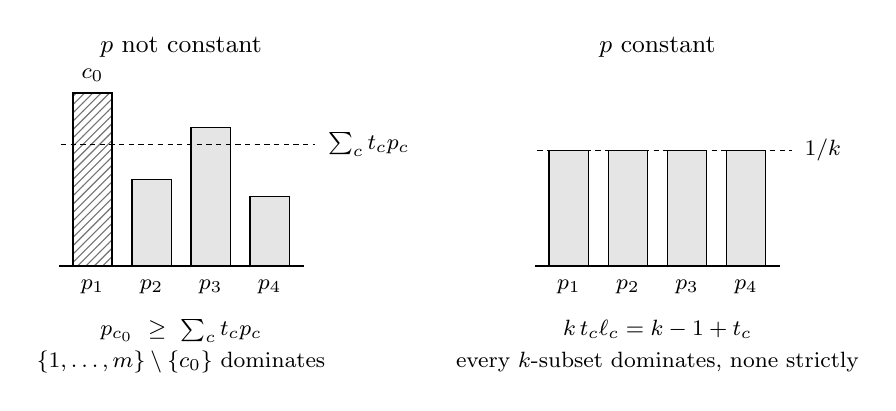
\begin{tikzpicture}[
  x=1cm, y=1cm,
  bar/.style={draw, line width=0.5pt, fill=black!10},
  hit/.style={draw, line width=0.7pt,
              pattern=north east lines, pattern color=black!55},
  mean/.style={dashed, dash pattern=on 1.9pt off 1.6pt, line width=0.55pt},
  every node/.style={font=\small}]

% ================= p not constant =========================================
\begin{scope}
  % heights are 4.4 p_c for p = (1/2, 1/4, 2/5, 1/5); the weighted mean is 7/20
  \draw[hit] (0.20,0) rectangle (0.70,2.20);
  \draw[bar] (0.95,0) rectangle (1.45,1.10);
  \draw[bar] (1.70,0) rectangle (2.20,1.76);
  \draw[bar] (2.45,0) rectangle (2.95,0.88);
  \draw[line width=0.6pt] (0.02,0)--(3.13,0);

  \draw[mean] (0.05,1.54)--(3.28,1.54);
  \node[anchor=west, font=\footnotesize] at (3.32,1.54) {$\sum_c t_cp_c$};

  \node[font=\footnotesize] at (0.45,2.42) {$c_0$};
  \foreach \x/\lab in {0.45/1, 1.20/2, 1.95/3, 2.70/4}
    {\node[anchor=north, font=\footnotesize] at (\x,-0.06) {$p_{\lab}$};}

  \node at (1.575,2.78) {$p$ not constant};
  \node[font=\footnotesize, align=center] at (1.575,-1.02)
    {$p_{c_0}\ \ge\ \sum_c t_cp_c$\\[2pt]
     $\{1,\dots,m\}\setminus\{c_0\}$ dominates};
\end{scope}

% ================= p constant =============================================
\begin{scope}[shift={(6.05,0)}]
  % every pivot equals 1/k with k = 3
  \draw[mean] (0.05,1.4667)--(3.28,1.4667);
  \node[anchor=west, font=\footnotesize] at (3.32,1.4667) {$1/k$};
  \foreach \x in {0.20, 0.95, 1.70, 2.45}
    {\draw[bar] (\x,0) rectangle (\x+0.50,1.4667);}
  \draw[line width=0.6pt] (0.02,0)--(3.13,0);

  \foreach \x/\lab in {0.45/1, 1.20/2, 1.95/3, 2.70/4}
    {\node[anchor=north, font=\footnotesize] at (\x,-0.06) {$p_{\lab}$};}

  \node at (1.575,2.78) {$p$ constant};
  \node[font=\footnotesize, align=center] at (1.575,-1.02)
    {$k\,t_c\ell_c=k-1+t_c$\\[2pt]
     every $k$-subset dominates, none strictly};
\end{scope}

\end{tikzpicture}

  \caption{Theorem~\ref{thm:corankone} at $(4,3)$.  The ratios $p_c$ of
  \eqref{eq:pvars} have co-weighted mean $1/k$ by \eqref{eq:pnorm}.  Left:
  the largest $p_{c_0}$ is at least the $t$-weighted mean $\sum_ct_cp_c$,
  so by \eqref{eq:corankone} its complement dominates.  Right: when $p$ is
  constant every $p_c$ equals $1/k$, the tie law \eqref{eq:tielaw} holds,
  every $k$-subset dominates and none dominates strictly.}
  \label{fig:jensen}
\end{figure}

Corank two is one further step: Corollary~\ref{cor:dualcell} converts it
into rank two, which is Theorem~\ref{thm:ranktwo}, and \S\ref{sec:corank}
carries out the conversion once that input is proved.

\section{The complex problem}\label{sec:complex}

Over $\C$ the problem is solved, and the answer stops exactly where the
elementary methods of \S\ref{sec:first}--\S\ref{sec:chart} stop:
$\GtzC(m,k)$ holds for $k\ge2$ if and only if $m\le k+1$.  Half of that
is already proved.  Nothing in \S\ref{sec:first} or \S\ref{sec:chart}
consulted the field, so their positive results stand over $\C$
unchanged, and they cover $m\le k+1$ (\S\ref{sec:cpositive}).

The other half needs one counterexample and a way to move it.  A single
design of size four and rank two fails, and two operations propagate the
failure across the board: one raises the size and the rank together, the
other raises the size alone, and each keeps a bound on the least
eigenvalue that any $k$-subset can achieve.

\subsection{The value of a design}\label{sec:cvalue}

Once the answer is \emph{no}, a number remains, and the operations of
\S\ref{sec:cpadding} propagate it.  Fix a
design $\dsn$ at $(m,k)$ over $\FF$.  For every $k$-subset $C$ and every
$x\in\FF^k$,
\begin{equation}\label{eq:cover}
  x\adj\SC x\;=\;\sum_{c\in C}\lvert\langle g_c,x\rangle\rvert^{2},
  \qquad\text{so}\qquad
  \SC\psd s\,I_k
  \iff
  s\lVert x\rVert^{2}\le\sum_{c\in C}\lvert\langle g_c,x\rangle\rvert^{2}
  \ \ \text{for all }x .
\end{equation}
Both readings are used below: the left one to recognize a design, the
right one to transport a bound along a map of index sets.  Put
\begin{equation}\label{eq:value}
  \operatorname{val}(\dsn)\;:=\;\max_{\lvert C\rvert=k}\lmin(\SC),
\end{equation}
a maximum over a finite set.  Since $\SC\psd sI_k$ is equivalent to
$\lmin(\SC)\ge s$, the design $\dsn$ admits a dominating $k$-subset if and
only if $\operatorname{val}(\dsn)\ge1$.
We say $\dsn$ \emph{has value at most} $b$ when $\SC-sI_k$ fails to be
positive semidefinite for every $k$-subset $C$ and every $s>b$; this is
$\operatorname{val}(\dsn)\le b$.  Finally set
\[
  \alpha_k(\FF)\;:=\;\inf_{m}\ \inf_{\dsn}\ \operatorname{val}(\dsn),
\]
the infimum over all sizes and all designs of size $m$ and rank $k$ over
$\FF$.  Thus $\Gtz(m,k)$ holds for every $m$ precisely when
$\alpha_k(\R)\ge1$, and likewise over $\C$; and since
Theorem~\ref{thm:corankone}(iii)--(iv) produces designs of value exactly
$1$ at every rank, the conjecture over $\R$ is the assertion
$\alpha_k(\R)=1$ for every $k$.

At every rank and over either field the value has a floor, which limits
how far the complex counterexamples can push it.

\begin{proposition}[Lean]\label{prop:rankfloor}
Every weighted design of size $m$ and rank $k$ over $\FF$ admits a
$k$-subset $C$ with $\SC\psd\frac1k I_k$.  Hence $\alpha_k(\FF)\ge1/k$.
\end{proposition}

\begin{proof}
Let $A$ be the $m\times k$ matrix whose $c$-th row is $g_c\adj$, so that
$(Ax)_c=\langle g_c,x\rangle$, and let $D=\diag(t_1,\dots,t_m)$.
Condition \eqref{eq:parseval} reads $A\adj DA=I_k$; in particular $A$ has
rank $k$, so some $k$-subset indexes an invertible $k\times k$ submatrix.
Choose $C$ maximizing $\lvert\det A_C\rvert$ among all $k$-subsets, put
$M:=A_C$ and $B:=AM^{-1}$.  Then $A=BM$, so the $c$-th row of $B$ holds
the coefficients expressing $g_c\adj$ in the rows of $M$, and the rows of
$B$ indexed by $C$ form $I_k$.  By Cramer's rule, $B_{ci}\det M$ is the
determinant of the matrix obtained from $M$ by substituting $g_c\adj$ for
its $i$-th row; that matrix is, up to a permutation of rows, $A_{C'}$ with
$C':=(C\setminus\{c_i\})\cup\{c\}$, where $c_i$ is the $i$-th element of
$C$; if $c$ already lies in $C\setminus\{c_i\}$ then that matrix has two
equal rows and its determinant vanishes.  Hence
\[
  \lvert B_{ci}\rvert\;=\;\frac{\lvert\det A_{C'}\rvert}{\lvert\det A_C\rvert}
  \;\le\;1
\]
for every $c$ and $i$, by maximality of the volume \cite{GT2001}.  By
Cauchy--Schwarz, for every $u\in\FF^k$,
\[
  \lvert (Bu)_c\rvert^{2}
  \;\le\;\Bigl(\sum_{i\le k}\lvert B_{ci}\rvert^{2}\Bigr)\lVert u\rVert^{2}
  \;\le\;k\lVert u\rVert^{2} .
\]
Fix $x\in\FF^k$ and take $u:=Mx$, so that $Ax=Bu$ and
$\lVert u\rVert^2=\sum_{c\in C}\lvert\langle g_c,x\rangle\rvert^2$.  Then
\[
  \lVert x\rVert^{2}
  \;=\;x\adj A\adj DAx
  \;=\;\sum_c t_c\lvert (Bu)_c\rvert^{2}
  \;\le\;k\lVert u\rVert^{2}\sum_c t_c
  \;=\;k\sum_{c\in C}\lvert\langle g_c,x\rangle\rvert^{2},
\]
which is \eqref{eq:cover} at $s=1/k$.
\end{proof}

\subsection{The positive half}\label{sec:cpositive}

\begin{proposition}[Lean]\label{prop:cpositive}
Let $k\ge1$ and $m\le k+1$.  Then $\GtzC(m,k)$ holds, as does
$\Gtz(m,k)$.
\end{proposition}

\begin{proof}
The vectors of a design span, so $m\ge k$ and there is nothing to prove
when $m<k$: no design exists.  If $m=k$ the assertion is
Proposition~\ref{prop:sizerank}, and if $m=k+1$ it is
Theorem~\ref{thm:corankone}.  Neither argument uses the field: the first
is the inequality $t_c\le1$ applied to \eqref{eq:parseval}, the second is
the rank-one Schur criterion together with the fact that a weighted mean
does not exceed its maximum.
\end{proof}

By Theorem~\ref{thm:corankone}(iii)--(iv) the bound $1$ is attained at
the last size at which it holds, and attained on a set of full dimension
in the weights: over either field and for every $k\ge1$, every weight
vector $t$ on $k+1$ atoms carries a design at $(k+1,k)$ in which every
$k$-subset dominates and none dominates strictly.  Its chart is
$P=I_{k+1}-zz\adj$ with
$\lvert z_c\rvert^{2}=(1-t_c)/k$, and its leverages obey the tie law
\eqref{eq:tielaw}.

One size lower the value overshoots: for $k\ge2$ every design at $(k,k)$
has value strictly above $1$, and $1$ is approached only as
$\max_c t_c\to1$.

\begin{proposition}\label{prop:square}
Let $\dsn$ be a design at $(k,k)$ over $\FF$.  Then $\ell_c=1/t_c$ for every
$c$, the unique $k$-subset satisfies
\[
  \lmin\bigl(S_{\{1,\dots,k\}}\bigr)\;=\;\frac{1}{\max_c t_c},
\]
and this quantity lies in $(1,k]$ for $k\ge2$.  Every weight vector is
realized, so for $k\ge2$ the infimum of $\operatorname{val}$ over designs
at $(k,k)$ equals $1$ and is not attained.
\end{proposition}

\begin{proof}
In the chart of \S\ref{sec:chart} the matrix $V$ is square with
$V\adj V=I_k$, hence unitary, so its rows are orthonormal:
$\langle v_c,v_d\rangle=\delta_{cd}$ with $v_c=\sqrt{t_c}\,g_c$.  Thus
$\ell_c=\lVert v_c\rVert^2/t_c=1/t_c$ and
\[
  S_{\{1,\dots,k\}}\;=\;\sum_c g_c^{\vphantom{\mathsf{H}}}g_c\adj
  \;=\;\sum_c \frac{1}{t_c}\,v_c^{\vphantom{\mathsf{H}}}v_c\adj,
\]
which is diagonal in the orthonormal basis $(v_c)$ with eigenvalues
$1/t_c$.  Its least eigenvalue is $1/\max_c t_c$.  Since $\sum_c t_c=1$
over $k\ge2$ terms, $1/k\le\max_c t_c<1$, whence the stated range.
Conversely $g_c:=t_c^{-1/2}e_c$ is a design at $(k,k)$ with weights $t$,
and letting $\max_c t_c\to1$ drives the value to $1$ from above.
\end{proof}

\subsection{The seed}\label{sec:cseed}

Let
$\omega:=e^{2\pi i/3}$, so that $1+\omega+\omega^{2}=0$ and
$\omega+\bar\omega=-1$.

\begin{example}[Lean]\label{ex:sic}
Put
\begin{equation}\label{eq:sic}
  g_0:=\bigl(\sqrt2,\,0\bigr),
  \qquad
  g_j:=\Bigl(\sqrt{\tfrac23},\ \sqrt{\tfrac43}\,\omega^{\,j-1}\Bigr)
  \quad(j=1,2,3),
  \qquad t_c:=\tfrac14 .
\end{equation}
Each vector has $\ell_c=2$: for $j\ge1$, $\tfrac23+\tfrac43=2$.  The atom
sum is
\[
  \sum_{j=1}^{3} g_j^{\vphantom{\mathsf{H}}}g_j\adj
  \;=\;\begin{pmatrix}2&\sqrt{8/9}\,\sum_j\overline{\omega^{\,j-1}}\\[2pt]
        \sqrt{8/9}\,\sum_j\omega^{\,j-1}&4\end{pmatrix}
  \;=\;\begin{pmatrix}2&0\\0&4\end{pmatrix},
\]
by $1+\omega+\omega^{2}=0$, so
$\sum_c g_c^{\vphantom{\mathsf{H}}}g_c\adj=4I_2$ and \eqref{eq:parseval} holds at
the uniform weight $\tfrac14$.  This is the $\C^2$ symmetric
informationally complete configuration: four equiangular lines, and indeed
$\lvert\langle g_a,g_b\rangle\rvert^{2}=\tfrac43$ for every $a\ne b$.  For
$b=0$ this is $(\sqrt2\cdot\sqrt{2/3})^2=4/3$; for
$1\le a<b\le3$ it is
\[
  \bigl(\tfrac23+\tfrac43\omega^{\,r}\bigr)
  \bigl(\tfrac23+\tfrac43\overline{\omega^{\,r}}\bigr)
  \;=\;\tfrac49-\tfrac89+\tfrac{16}9\;=\;\tfrac43,
  \qquad r=b-a\not\equiv0,
\]
using $\omega^{r}+\overline{\omega^{r}}=-1$.
\end{example}

\begin{lemma}[Lean]\label{lem:sicvalue}
The design \eqref{eq:sic} has value exactly
\[
  \alpha_{\mathrm{SIC}}\;:=\;2-\frac{2}{\sqrt3}\;=\;0.8452994616\ldots,
\]
the least root of $z^{2}-4z+\tfrac83$.  In particular $\GtzC(4,2)$ is
false, and $\alpha_2(\C)\le\alpha_{\mathrm{SIC}}<\tfrac9{10}$.
\end{lemma}

\begin{proof}
Let $C=\{a,b\}$ be a pair and let $A$ be the $2\times2$ matrix with rows
$g_a\adj,g_b\adj$, so that $\SC=A\adj A$ and
\[
  \det\SC=\lvert\det A\rvert^{2}=\det AA\adj
  =\ell_a\ell_b-\lvert\langle g_a,g_b\rangle\rvert^{2}
  =4-\tfrac43=\tfrac83 ,
  \qquad \tr\SC=\ell_a+\ell_b=4 .
\]
Hence $\det(\SC-zI_2)=z^{2}-4z+\tfrac83$ for every one of the six pairs,
with roots $2\pm2/\sqrt3$, and $\lmin(\SC)=\alpha_{\mathrm{SIC}}$.  The value is the
maximum of these six equal numbers.  Since $\alpha_{\mathrm{SIC}}<1$ no pair dominates.
The inequality $\alpha_{\mathrm{SIC}}<\tfrac9{10}$ is $\tfrac{11}{10}<\tfrac2{\sqrt3}$,
that is $11\sqrt3<20$, that is $363<400$.
\end{proof}

Here the two fields part: over $\R$ rank two holds at every size
(Theorem~\ref{thm:ranktwo}), so $\alpha_2(\R)=1$, while over $\C$ the
same cell has value below $1$ already at size four.  No proof of $\Gtz$
can therefore be field-agnostic.  The constant $\alpha_{\mathrm{SIC}}$
is moreover sharp: by \cite{Nesterenko2026complex} no uniform-weight
design of rank two has value below $2-2/\sqrt3$, the bound being attained exactly when
$4\mid m$, at a repeated copy of \eqref{eq:sic}.  The bound passes to
arbitrary weights in two steps.  Merging equal vectors turns a uniform
design of larger size into one with rational weights, so by
Lemma~\ref{lem:split} read backwards it has the same value and the bound
holds there.  For arbitrary weights, hold the chart $P$ fixed: by
Lemma~\ref{lem:realize} every weight vector $t'$ with positive entries
carries a design with that chart, namely $g'_c=\sqrt{t_c/t'_c}\,g_c$, and
$\operatorname{val}$ is a continuous function of $t'$ there, being a
maximum of finitely many least eigenvalues of matrices depending
continuously on $t'$.  Rational weight vectors are dense in the open
simplex, so the bound persists in the limit.  Hence
$\alpha_2(\C)=2-2/\sqrt3$.

\subsection{Two padding operations}\label{sec:cpadding}

The first operation adjoins one coordinate together with one atom along
it, raising the size and the rank by one.  The second lists an existing
atom twice, raising the size alone.  Each preserves \eqref{eq:parseval}
by a one-line computation, and each preserves a value bound.

\begin{lemma}[Lean]\label{lem:spike}
Let $\dsn$ be a complex weighted design at $(m,k)$ and let $0<w<1$.  Define
$\widehat{\dsn}$ at $(m+1,k+1)$ by
\begin{equation}\label{eq:spike}
  \widehat g_c:=\Bigl(\frac{g_c}{\sqrt{1-w}},\,0\Bigr)\ \ (c\le m),
  \qquad
  \widehat g_{m+1}:=\frac{1}{\sqrt w}\,e_{k+1},
  \qquad
  \widehat t_c:=(1-w)t_c,\quad \widehat t_{m+1}:=w .
\end{equation}
Then $\widehat{\dsn}$ is a design, and if $\dsn$ has value at most $b\ge0$ then
$\widehat{\dsn}$ has value at most $b/(1-w)$.
\end{lemma}

\begin{proof}
The weights are positive and sum to $(1-w)+w=1$.  For the Parseval
condition, the first $m$ terms contribute
\[
  \sum_{c\le m}(1-w)t_c\,
  \frac{1}{1-w}\begin{pmatrix}g_c^{\vphantom{\mathsf{H}}}g_c\adj&0\\0&0\end{pmatrix}
  \;=\;\begin{pmatrix}I_k&0\\0&0\end{pmatrix},
\]
and the last contributes $w\cdot w^{-1}e_{k+1}^{\vphantom{\mathsf{H}}}e_{k+1}\adj$;
the sum is $I_{k+1}$.

Now let $C$ be a $(k+1)$-subset and $s>b/(1-w)$; we show $S_C-sI_{k+1}$ is
not positive semidefinite.  Suppose first $m+1\notin C$.  Every
$\widehat g_c$ with $c\le m$ vanishes in the last coordinate, so the
$(k+1,k+1)$ entry of $S_C-sI_{k+1}$ is $-s<0$, and a positive semidefinite
matrix has nonnegative diagonal.  Suppose instead $m+1\in C$ and put
$C':=C\setminus\{m+1\}$, a $k$-subset of $\{1,\dots,m\}$.  Test on the
flat directions $\widehat x:=(x,0)$ with $x\in\C^k$.  There
\[
  \langle\widehat g_{m+1},\widehat x\rangle=0,
  \qquad
  \langle\widehat g_c,\widehat x\rangle
  =\frac{\langle g_c,x\rangle}{\sqrt{1-w}}\quad(c\le m),
  \qquad
  \lVert\widehat x\rVert=\lVert x\rVert .
\]
If $S_C\psd sI_{k+1}$ then, by the right-hand form of \eqref{eq:cover}
applied to $\widehat x$,
\[
  s\lVert x\rVert^{2}
  \;\le\;\sum_{c\in C}\lvert\langle\widehat g_c,\widehat x\rangle\rvert^{2}
  \;=\;\frac{1}{1-w}\sum_{c\in C'}\lvert\langle g_c,x\rangle\rvert^{2}
  \qquad\text{for every }x\in\C^{k},
\]
that is $S_{C'}\psd (1-w)s\,I_k$ in the original design.  But
$(1-w)s>b$, contradicting the hypothesis on $\dsn$.
\end{proof}

The spike is invisible in the flat directions and is the only atom
visible in the new one.  The factor $1/(1-w)$ costs something real: for
$b>0$ every admissible $w$ has $b<b/(1-w)$, so no member of the family
attains the level $b$, though the levels descend to it as $w\to0$.

\begin{lemma}[Lean]\label{lem:split}
Let $\dsn$ be a complex weighted design at $(m,k)$, let $c_0\le m$ and let
$0<f<1$.  Define $\widetilde{\dsn}$ at $(m+1,k)$ by listing the vector
$g_{c_0}$ twice,
\begin{equation}\label{eq:split}
  \widetilde g_c:=g_c\ (c\le m),
  \quad \widetilde g_{m+1}:=g_{c_0},
  \qquad
  \widetilde t_{c_0}:=f\,t_{c_0},
  \quad \widetilde t_{m+1}:=(1-f)t_{c_0},
  \quad \widetilde t_c:=t_c\ \text{otherwise.}
\end{equation}
Then $\widetilde{\dsn}$ is a design, and if $\dsn$ has value at most $b\ge0$ then
so does $\widetilde{\dsn}$.
\end{lemma}

\begin{proof}
The weights are positive and still sum to one, and in
\eqref{eq:parseval} the term $t_{c_0}g_{c_0}^{\vphantom{\mathsf{H}}}g_{c_0}\adj$ is
replaced by
$f t_{c_0}g_{c_0}^{\vphantom{\mathsf{H}}}g_{c_0}\adj+(1-f)t_{c_0}
g_{c_0}^{\vphantom{\mathsf{H}}}g_{c_0}\adj$, which is the same matrix.

Let $C$ be a $k$-subset of $\{1,\dots,m+1\}$ and $s>b\ge0$.  If $C$ fails
to contain both labels $c_0$ and $m+1$, then replacing $m+1$ by $c_0$ where
necessary carries $C$ to a $k$-subset $C'$ of $\{1,\dots,m\}$ with the
same family of vectors, so $S_C=S_{C'}$ and $S_C-sI_k$ is not positive
semidefinite by the hypothesis on $\dsn$.  If $C$ contains both labels, its
$k$ vectors include two equal ones, hence span a subspace of dimension at
most $k-1$; choosing $x\ne0$ orthogonal to that subspace gives
$x\adj S_Cx=0$ by \eqref{eq:cover}, while
$x\adj(sI_k)x=s\lVert x\rVert^{2}>0$.
\end{proof}

\subsection{The ladder}\label{sec:cladder}

\begin{theorem}[Lean]\label{thm:ladder}
Let $k\ge2$ and $m\ge k+2$.  There is a complex weighted design of size
$m$ and rank $k$ whose value is at most
\[
  \tfrac{10}9\,\alpha_{\mathrm{SIC}}\;=\;\frac{20}{9}-\frac{20\sqrt3}{27}
  \;=\;0.9392216240\ldots\;<\;1 .
\]
In particular $\GtzC(m,k)$ is false.
\end{theorem}

\begin{proof}
Set $e:=k-2\ge0$.  If $e=0$ start with the design \eqref{eq:sic} itself,
of size $4=k+2$ and value $\alpha_{\mathrm{SIC}}$ by Lemma~\ref{lem:sicvalue}.  If
$e\ge1$, apply Lemma~\ref{lem:spike} $e$ times to \eqref{eq:sic} with the
common spike weight
\[
  w\;:=\;1-\Bigl(\tfrac9{10}\Bigr)^{1/e},
  \qquad\text{so that}\qquad (1-w)^{e}=\tfrac9{10}.
\]
Each application raises the size and the rank by one, so after $e$ steps
the size is $4+e=k+2$ and the rank is $2+e=k$; and each application
divides the value bound by $1-w$, so the resulting bound is
\[
  \frac{\alpha_{\mathrm{SIC}}}{(1-w)^{e}}\;=\;\frac{10}{9}\,\alpha_{\mathrm{SIC}} .
\]
This is the asserted bound, and it is below $1$ because
$\alpha_{\mathrm{SIC}}<\tfrac9{10}$ (Lemma~\ref{lem:sicvalue}).  Finally apply
Lemma~\ref{lem:split} $m-k-2$ times, which raises the size to $m$ without
raising the rank and without raising the value bound.  A design of value
below $1$ has no dominating $k$-subset.
\end{proof}

At $k=3$ the theorem is the one-spike padded configuration of size five,
whose value is exactly $\tfrac{10}9\alpha_{\mathrm{SIC}}$; that cell, $(5,3)$, is the
smallest at which rank three fails over $\C$, since
Proposition~\ref{prop:cpositive} covers $m\le4$.  The bound is not the
best available at larger sizes: \S\ref{sec:csharp} exhibits designs of
rank three with value $0.7639\ldots$ and $0.7018\ldots$.

\begin{theorem}[Lean]\label{thm:complex}
Let $k\ge2$.  Then
\[
  \GtzC(m,k)\quad\Longleftrightarrow\quad m\le k+1 .
\]
For $k\le1$, $\GtzC(m,k)$ holds for every $m$.
\end{theorem}

\begin{proof}
For $m\le k+1$ this is Proposition~\ref{prop:cpositive}; for $m\ge k+2$ it
is Theorem~\ref{thm:ladder}.  At $k=1$ the statement is
Proposition~\ref{prop:rankone}, and at $k=0$ the empty subset dominates
the $0\times0$ identity.
\end{proof}

For $k\ge2$ the equivalence is vacuous below $m=k$, where Parseval admits
no design: the assertion holds there for want of anything to
quantify over, not because selection succeeds.

\subsection{The sharp constants}\label{sec:csharp}

Theorem~\ref{thm:complex} settles the decision problem over $\C$ and
leaves the quantitative one.  By Proposition~\ref{prop:rankfloor} and
Theorem~\ref{thm:ladder},
\[
  \frac1k\;\le\;\alpha_k(\C)\;\le\;\frac{10}{9}\alpha_{\mathrm{SIC}}\;<\;1
  \qquad(k\ge2),
\]
and at rank two both ends are known: $\alpha_2(\C)=2-2/\sqrt3$, the upper
bound by Lemma~\ref{lem:sicvalue} and the lower by
\cite{Nesterenko2026complex}.  At rank three the two ends are far apart, and two designs push the
upper end below the padded seed.

\begin{example}[Lean]\label{ex:trine}
Two coplanar trines of lines in $\C^{3}$ sharing an axis: for $j=0,1,2$,
\[
  g_j:=\bigl(\sqrt2,\,0,\,\omega^{\,j}\bigr),
  \qquad
  g_{3+j}:=\bigl(0,\,\sqrt2,\,\omega^{\,j}\bigr),
  \qquad t_c:=\tfrac16 .
\]
Every leverage is $2+1=3$, and
$\sum_{j}g_j^{\vphantom{\mathsf{H}}}g_j\adj=\diag(6,0,3)$,
$\sum_{j}g_{3+j}^{\vphantom{\mathsf{H}}}g_{3+j}\adj=\diag(0,6,3)$, the off-diagonal
entries cancelling by $1+\omega+\omega^{2}=0$; the total is $6I_3$, so
\eqref{eq:parseval} holds.  This design has value exactly $3-\sqrt5$.
\end{example}

To prove the last assertion, and to prepare the rank-three record, we
compute the determinant of a triple once and for all.  Let $C=\{a,b,c\}$ and let $A$ be the
$3\times3$ matrix with rows $g_a\adj,g_b\adj,g_c\adj$.  Then $\SC=A\adj A$
while the Gram matrix is $\Gram_C=AA\adj$, with entries
$\langle g_i,g_j\rangle$; for square $A$ the two have the same
characteristic polynomial.  Writing $\beta_{ij}:=\langle g_i,g_j\rangle$
and expanding the $3\times3$ determinant of
$\Gram_C-sI_3$ gives, with $d:=3-s$ when all three leverages equal $3$,
\begin{equation}\label{eq:tripledet}
  \det(\SC-sI_3)
  \;=\;d^{3}
      -d\bigl(\lvert\beta_{ab}\rvert^{2}+\lvert\beta_{bc}\rvert^{2}
              +\lvert\beta_{ca}\rvert^{2}\bigr)
      +2\operatorname{Re}\beta_{abc},
  \qquad
  \beta_{abc}:=\beta_{ab}\beta_{bc}\beta_{ca}.
\end{equation}
The three moduli form a phase-free budget, and the phases enter through
the single real number $\operatorname{Re}\beta_{abc}$, affinely.

For the trine, the two coplanar triples $\{g_0,g_1,g_2\}$ and
$\{g_3,g_4,g_5\}$ have atom sums $\diag(6,0,3)$ and $\diag(0,6,3)$, of
least eigenvalue $0$.  Every other triple consists of two vectors from one
side and one from the other, say $g_i,g_j,g_{3+l}$ with $i\ne j$; then
\[
  \beta_{ij}=2+\omega^{\,j-i},
  \qquad
  \beta_{j,3+l}=\omega^{\,l-j},
  \qquad
  \beta_{3+l,i}=\omega^{\,i-l},
\]
so the budget is $\lvert2+\omega^{\,j-i}\rvert^{2}+1+1=3+2=5$ and
\[
  \beta_{abc}=(2+\omega^{\,j-i})\,\omega^{\,i-j}=2\omega^{\,i-j}+1,
  \qquad \operatorname{Re}\beta_{abc}=1+2\cdot(-\tfrac12)=0 .
\]
By \eqref{eq:tripledet}, $\det(\SC-sI_3)=d^{3}-5d=d(d^{2}-5)$, so the
spectrum of $\SC$ is $\{3,\,3-\sqrt5,\,3+\sqrt5\}$ and
$\lmin(\SC)=3-\sqrt5=0.7639320225\ldots$ for all eighteen such triples.
The value of the design is the maximum over the twenty triples, namely
$3-\sqrt5$.  In particular $\GtzC(6,3)$ fails, at a level well below the
one Theorem~\ref{thm:ladder} provides.

\begin{example}[Lean]\label{ex:hesse}
The Hesse configuration.  Index nine directions of $\C^{3}$ by a slot
$p\in\{0,1,2\}$ and a phase $q\in\{0,1,2\}$: the direction $u_{3p+q}$
carries $0$ in slot $p$, $\omega^{q}$ in slot $p+1$ and $-\omega^{2q}$ in
slot $p+2$, indices modulo three.  Explicitly, with $\omega$ written $w$,
\[
  \begin{array}{lll}
    u_0=(0,1,-1), & u_3=(-1,0,1), & u_6=(1,-1,0),\\
    u_1=(0,w,-w^{2}), & u_4=(-w^{2},0,w), & u_7=(w,-w^{2},0),\\
    u_2=(0,w^{2},-w), & u_5=(-w,0,w^{2}), & u_8=(w^{2},-w,0).
  \end{array}
\]
Each $u_c$ has $\lVert u_c\rVert^{2}=2$, and
$\sum_c u_c^{\vphantom{\mathsf{H}}}u_c\adj=6I_3$: the family $p$ contributes $1$ to
each of the diagonal slots $p+1$ and $p+2$ for each of its three phases,
so every slot receives $6$ from the two families that do not vanish there,
while its one off-diagonal entry,
$\omega^{q}\overline{(-\omega^{2q})}=-\omega^{-q}$ in position
$(p+1,p+2)$, sums to $-\sum_q\omega^{-q}=0$ over the family.  Put
\[
  g_c:=\sqrt{\tfrac32}\,u_c,\qquad t_c:=\tfrac19 .
\]
Then \eqref{eq:parseval} holds, $\ell_c=3$ for every $c$, and for $a\ne b$
\[
  \langle u_a,u_b\rangle^{3}=-1,
  \qquad\text{hence}\qquad
  \beta_{ab}^{3}=\langle g_a,g_b\rangle^{3}=-\tfrac{27}8 .
\]
The overlap identity is two computations.  Within the family $p$, with
$r:=q'-q\not\equiv0$,
\[
  \langle u_{3p+q},u_{3p+q'}\rangle=\omega^{r}+\omega^{2r}=-1 ;
\]
and between the families $p$ and $p+1$ the only slot on which both are
nonzero is $p+2$, so
\[
  \langle u_{3p+q},u_{3(p+1)+q'}\rangle
  =\overline{(-\omega^{2q})}\,\omega^{q'}=-\omega^{\,q+q'} .
\]
Each value is $-1$ times a cube root of unity, hence a cube root of $-1$;
the remaining pairs are the conjugates of these.
\end{example}

Since $\lvert\beta_{ab}\rvert^{2}$ is a nonnegative real whose cube is
$\lvert\beta_{ab}^{3}\rvert^{2}=(27/8)^{2}$, it equals $9/4$; the
configuration is equiangular, and the budget in \eqref{eq:tripledet} is
$3\cdot\tfrac94=\tfrac{27}4$ for every triple.  The triangle invariant
satisfies $\beta_{abc}^{3}=(\beta_{ab}\beta_{bc}\beta_{ca})^{3}=-(27/8)^{3}$, so $\beta_{abc}$
is one of the three cube roots of $-(27/8)^3$, namely $-\tfrac{27}8$ and
$\tfrac{27}{16}(1\pm i\sqrt3)$.  Hence
\begin{equation}\label{eq:hessedet}
  \det(\SC-sI_3)\;=\;(3-s)^{3}-\tfrac{27}4(3-s)+2\operatorname{Re}\beta_{abc},
  \qquad \operatorname{Re}\beta_{abc}\in\Bigl\{-\tfrac{27}8,\ \tfrac{27}{16}\Bigr\},
\end{equation}
the first alternative occurring exactly when $\det\SC=\tfrac{27}4+2\operatorname{Re}\beta_{abc}$
vanishes, i.e.\ for the twelve triples lying on a line of the Hesse
configuration, and the second for the remaining seventy-two.  With
$\operatorname{Re}\beta_{abc}=\tfrac{27}{16}$ the right-hand side of
\eqref{eq:hessedet} expands to
\begin{equation}\label{eq:hessecubic}
  \det(\SC-sI_3)\;=\;-\tfrac18\,h(s),
  \qquad
  h(s):=8s^{3}-72s^{2}+162s-81 ,
\end{equation}
and with $\operatorname{Re}\beta_{abc}=-\tfrac{27}8$ it is $-s(s-\tfrac92)^{2}$.

\begin{proposition}[Lean]\label{prop:hesse}
The roots of $h$ are $3(1-\cos\tfrac{2\pi}9)$,
$3(1-\cos\tfrac{4\pi}9)$ and $3(1-\cos\tfrac{8\pi}9)$.  The design of
Example~\ref{ex:hesse} has value exactly
\[
  h_3\;:=\;3\Bigl(1-\cos\tfrac{2\pi}9\Bigr)\;=\;0.7018666706\ldots
\]
Consequently $\alpha_3(\C)\le h_3$, and $\GtzC(m,3)$ fails for every
$m\ge5$.
\end{proposition}

\begin{proof}
Substituting $s=3(1-\gamma)$ in \eqref{eq:hessecubic} gives
\[
  h\bigl(3(1-\gamma)\bigr)\;=\;-27\bigl(8\gamma^{3}-6\gamma+1\bigr),
\]
and for $\gamma=\cos\theta$ the identity $4\cos^{3}\theta-3\cos\theta
=\cos3\theta$ turns $8\gamma^{3}-6\gamma+1=0$ into
$\cos3\theta=-\tfrac12$.  As $\theta$ runs over $[0,\pi]$ the angle
$3\theta$ runs over $[0,3\pi]$, where the cosine takes the value
$-\tfrac12$ at $\tfrac{2\pi}3$, $\tfrac{4\pi}3$ and $\tfrac{8\pi}3$; the
solutions are therefore
$\theta=\tfrac{2\pi}9,\tfrac{4\pi}9,\tfrac{8\pi}9$, which gives the three
roots.  They are distinct, and $s=3(1-\cos\theta)$ increases with $\theta$,
so $h_3$ is the least.  Exact evaluation isolates it: $h$ is negative at
$\tfrac7{10}$, where its value is $-\tfrac{136}{1000}$, and positive at
$\tfrac{71}{100}$, where its value is $\tfrac{588088}{10^{6}}$, so
\begin{equation}\label{eq:hessewindow}
  \tfrac7{10}\;<\;h_3\;<\;\tfrac{71}{100}.
\end{equation}

By \eqref{eq:hessecubic} the seventy-two nondegenerate triples all have
characteristic polynomial $-\tfrac18h$, hence
$\lmin(\SC)=h_3$ for each; the twelve degenerate triples have
$\lmin(\SC)=0$.  The value is the maximum, $h_3$.  By
\eqref{eq:hessewindow}, $h_3<1$, so no triple
dominates, so $\GtzC(9,3)$ fails; Lemma~\ref{lem:split} propagates the
failure to every $m\ge9$, and Theorem~\ref{thm:ladder} covers
$5\le m\le8$.
\end{proof}

An explicit certificate can replace the eigenvalue computation,
exhibiting positive semidefiniteness at the threshold without reference
to the spectral theorem.  Take the triple $\{u_0,u_1,u_3\}$.
From $1+\omega+\omega^{2}=0$,
\[
  u_0^{\vphantom{\mathsf{H}}}u_0\adj+u_1^{\vphantom{\mathsf{H}}}u_1\adj
  +u_3^{\vphantom{\mathsf{H}}}u_3\adj
  \;=\;\begin{pmatrix}1&0&-1\\0&2&\omega\\-1&\omega^{2}&3\end{pmatrix},
\]
so that $\SC$ is $\tfrac32$ times this matrix.  Writing
$p:=\tfrac32-s$ and $q:=3-s$ and $\operatorname{atom}(v):=vv\adj$, a
direct expansion of both sides gives the polynomial identity
\begin{equation}\label{eq:hesseldl}
  pq\,\bigl(\SC-sI_3\bigr)
  \;=\;q\cdot\operatorname{atom}\bigl(p,0,-\tfrac32\bigr)
      +p\cdot\operatorname{atom}\bigl(0,q,\tfrac32\omega^{2}\bigr)
      -\tfrac18h(s)\,E_{33},
\end{equation}
$E_{33}$ being the matrix unit in the last diagonal slot.  The identity is
the $LDL\adj$ factorization of $\SC-sI_3$ cleared of denominators: the
leading $2\times2$ block of $\SC-sI_3$ is the diagonal $\diag(p,q)$, the
two rank-one terms are the pivot contributions of that factorization
multiplied by $pq$, and the coefficient of $E_{33}$ is $pq$ times the
Schur complement of the block, which is where $h$ enters.  Checking the
identity is a computation: the entries other than $(3,3)$ agree as
polynomials in $s$, and the residue at $(3,3)$ is
\[
  pq\bigl(\tfrac92-s\bigr)-\tfrac94(p+q)
  \;=\;\Bigl(-s^{3}+9s^{2}-\tfrac{99}4s+\tfrac{81}4\Bigr)
        -\Bigl(\tfrac{81}8-\tfrac92 s\Bigr)
  \;=\;-\tfrac18h(s).
\]
At $s=h_3$ the cubic vanishes and both $p$ and $q$ are positive, since
$h_3<\tfrac{71}{100}<\tfrac32$; dividing \eqref{eq:hesseldl} by the
positive scalar $pq$ exhibits $\SC-h_3I_3$ as a nonnegative combination of
two rank-one positive semidefinite matrices.  The threshold $h_3$ is
therefore attained by this triple.

The three complex records at rank three are ordered
\[
  h_3=0.7018666706\ldots
  \;<\;3-\sqrt5=0.7639320225\ldots
  \;<\;\tfrac{10}9\alpha_{\mathrm{SIC}}=0.9392216240\ldots ,
\]
both inequalities being exact.  For the second, $12<7\sqrt3$ gives
$\alpha_{\mathrm{SIC}}>\tfrac56$ and hence $\tfrac{10}9\alpha_{\mathrm{SIC}}>\tfrac{25}{27}$, while
$5>\bigl(\tfrac{223}{100}\bigr)^{2}$ gives $3-\sqrt5<\tfrac{77}{100}$, and
$2500>2079$.  For the first,
\[
  h\bigl(3-\sqrt5\bigr)\;=\;\bigl(576-1008+486-81\bigr)
   +\bigl(-256+432-162\bigr)\sqrt5\;=\;14\sqrt5-27\;>\;0,
\]
since $980>729$.  The three roots of $h$ sum to $9$, so they cannot all
lie below $2$; with $h(2)=19>0$ this places $2$ strictly between the two
smallest roots.  As $3-\sqrt5<2$ and $h(3-\sqrt5)>0$, the number
$3-\sqrt5$ lies in the same interval, hence above $h_3$.

\begin{remark}\label{rem:phase}
Identity \eqref{eq:tripledet} shows where the two fields differ.
Over $\R$ the entries $\beta_{ij}$ are real, so $\beta_{abc}$ is real and
$\operatorname{Re}\beta_{abc}=\pm\lvert\beta_{abc}\rvert$ is forced to an extreme of its
range; over $\C$ it may sit anywhere in
$[-\lvert\beta_{abc}\rvert,\lvert\beta_{abc}\rvert]$, and the separating
quantity is the phase defect
$\lvert\beta_{abc}\rvert^{2}-(\operatorname{Re}\beta_{abc})^{2}=(\operatorname{Im}\beta_{abc})^{2}$,
which vanishes identically for every real configuration.  The trine of
Example~\ref{ex:trine} isolates the mechanism: its
modulus budget $5$ would permit $2\operatorname{Re}\beta_{abc}=2\sqrt3$ and hence a
positive determinant at $s=1$, but its phase defect is $3$ and its
$\operatorname{Re}\beta_{abc}$ is $0$, leaving $\det(\SC-I_3)=-2$.  No
argument that sees only the moduli $\lvert\beta_{ij}\rvert$ can decide
either problem; the corresponding no-go statement is recorded in
Appendix~\ref{app:graveyard}.
\end{remark}

\begin{remark}\label{rem:sharpc}
Collecting the two ends,
\[
  \tfrac13\;\le\;\alpha_3(\C)\;\le\;3\bigl(1-\cos\tfrac{2\pi}{9}\bigr)
  \;=\;0.7018\ldots,
\]
the lower bound from Proposition~\ref{prop:rankfloor} and the upper from
Proposition~\ref{prop:hesse}.  The gap stays open: every rank-three
statement above bounds $\alpha_3(\C)$ from above, and such bounds move
the record down without pinning it.  Determining $\alpha_3(\C)$ is
Problem~\ref{prob:sharpc}.  The rank-inverse bound $1/k$ is sharp only at
$k=1$, where the one-atom design at $(1,1)$ has value $1$.
\end{remark}

\section{The real problem: decided cells}\label{sec:real}

Over $\R$ the mechanisms of \S\ref{sec:first} decide rank one and the
square $m=k$, and duality (Theorem~\ref{thm:duality}) converts corank one
and corank two into rank one and rank two.  Missing are rank two itself and any control on the size.  This section
supplies both by the same device: an operation producing from a design
a smaller design whose dominating subsets transport back.

Deleting a vector of length at most one (\S\ref{sec:light}) lowers the
size by one but moves the remaining vectors, by a congruence; the
transport back is then an identity between quadratic forms, and it is
available only because the deleted vector was short.  Carathéodory
reduction (\S\ref{sec:crystal}) lowers the size to at most $k(k+1)/2+1$
and leaves the vectors where they are; the transport back is immediate,
because $\SC$ in \eqref{eq:dominate} does not involve the weights.  The first operation stalls when every vector is long, and rank two is
where the stalled case can be settled outright
(\S\ref{sec:ranktwo}).

\subsection{Deleting a light vector}\label{sec:light}

\begin{definition}\label{def:light}
A vector of a design is \emph{light} if $\ell_c\le1$ and \emph{heavy} if
$\ell_c>1$.  The design is \emph{all-heavy} if every one of its vectors is
heavy.
\end{definition}

By Lemma~\ref{lem:trace} the $t$-weighted mean of the $\ell_c$ equals $k$,
so at rank $k\ge2$ a design always has a heavy vector; whether it has a
light one is the dichotomy exploited here.  The elementary fact behind the
deletion is the rank-one criterion
\begin{equation}\label{eq:schurone}
  I_k-g^{\vphantom{\mathsf{T}}}g\tp\psd0
  \quad\Longleftrightarrow\quad
  \lVert g\rVert^2\le1 ,
\end{equation}
whose forward direction is the value of the form at $g$, namely
$\lVert g\rVert^2(1-\lVert g\rVert^2)$, and whose converse is
Cauchy--Schwarz: $\langle g,u\rangle^2\le\lVert g\rVert^2\lVert
u\rVert^2\le\lVert u\rVert^2$.

\begin{theorem}[Lean]\label{thm:light}
Let $m\ge2$ and let $\dsn$ be a design at $(m,k)$ possessing a light vector.
If $\Gtz(m-1,k)$ holds, then $\dsn$ admits a dominating $k$-subset.
\end{theorem}

\begin{proof}
Let $\ell_d\le1$.  Since $m\ge2$ and all weights are positive with
$\sum_ct_c=1$, we have $t_d<1$.

\emph{Step 1: the residual Parseval mass is positive definite.}  Put
$\Sigma_d:=I_k-t_d\,g_d^{\vphantom{\mathsf{T}}}g_d\tp$, which by \eqref{eq:parseval} is
$\sum_{c\ne d}t_c\,g_c^{\vphantom{\mathsf{T}}}g_c\tp$.  For $u\ne0$,
\[
  u\tp \Sigma_d u=\lVert u\rVert^2-t_d\langle g_d,u\rangle^2
  \;\ge\;(1-t_d\ell_d)\lVert u\rVert^2\;>\;0 ,
\]
using Cauchy--Schwarz and $t_d\ell_d\le t_d<1$.  Write $\Sigma_d=LL\tp$ with $L$
invertible and set $R:=L^{-\mathsf{T}}$, so that
\begin{equation}\label{eq:whiten}
  R\tp \Sigma_d R=I_k ,\qquad \det R\ne0 .
\end{equation}

\emph{Step 2: the deflated design.}  On the index set
$E:=\{1,\dots,m\}\setminus\{d\}$ put
\[
  g'_c:=\sqrt{1-t_d}\;R\tp g_c ,
  \qquad
  t'_c:=\frac{t_c}{1-t_d}
  \qquad (c\in E).
\]
The weights are positive and sum to one, because
$\sum_{c\in E}t_c=1-t_d$.  For the Parseval condition the factor
$1-t_d$ cancels against the reweighting, and the congruence identity
$(R\tp g)(R\tp g)\tp=R\tp(g^{\vphantom{\mathsf{T}}}g\tp)R$ gives
\[
  \sum_{c\in E}t'_c\,(g'_c)(g'_c)\tp
  \;=\;\sum_{c\in E}t_c\,R\tp g_c^{\vphantom{\mathsf{T}}}g_c\tp R
  \;=\;R\tp \Sigma_d R\;=\;I_k
\]
by \eqref{eq:whiten}.  So $\bigl((g'_c),(t'_c)\bigr)$ is a design at
$(m-1,k)$.

\emph{Step 3: transport.}  By hypothesis some $C\subseteq E$ with
$\lvert C\rvert=k$ dominates in the deflated design.  Its subset sum is
$\sum_{c\in C}(g'_c)(g'_c)\tp=(1-t_d)R\tp\SC R$, so
domination reads
\[
  R\tp\bigl((1-t_d)\SC-\Sigma_d\bigr)R\;\psd\;0 ,
\]
and congruence by the invertible $R$ gives $(1-t_d)\SC-\Sigma_d\psd0$.  The
identity
\begin{equation}\label{eq:reassemble}
  \SC-I_k
  \;=\;\frac{1}{1-t_d}\Bigl[\bigl((1-t_d)\SC-\Sigma_d\bigr)
        \;+\;t_d\bigl(I_k-g_d^{\vphantom{\mathsf{T}}}g_d\tp\bigr)\Bigr]
\end{equation}
is verified by expanding $\Sigma_d$: the two occurrences of
$t_d\,g_d^{\vphantom{\mathsf{T}}}g_d\tp$ cancel and the bracket equals
$(1-t_d)(\SC-I_k)$.  Its first summand is positive semidefinite by the
previous display, its second by \eqref{eq:schurone} and $\ell_d\le1$, and
the scalar is positive.  Hence $C$ dominates in $\dsn$.
\end{proof}

Lightness enters only in the second summand of \eqref{eq:reassemble};
the rest is the congruence and its bookkeeping.  Iterating the theorem removes light vectors one at a time:

\begin{corollary}[Lean]\label{cor:heavy}
Let $k\ge1$.  If every all-heavy design of rank $k$, of whatever size,
admits a dominating $k$-subset, then $\Gtz(m,k)$ holds for every $m$.
\end{corollary}

\begin{proof}
Strong induction on $m$.  A design at $(m,k)$ has $m\ge k$.  If $m=k$,
apply Proposition~\ref{prop:sizerank}.  If $m>k$ and some vector is light,
then $m-1\ge k\ge1$ and $m\ge2$, so Theorem~\ref{thm:light} applies with
the induction hypothesis $\Gtz(m-1,k)$.  Otherwise the design is
all-heavy and the assumption applies.
\end{proof}

The tetrahedron of Example~\ref{ex:tetra} has $\ell_c=3$ for every $c$ and
is therefore all-heavy: the deletion is unavailable precisely at the
design where, by Example~\ref{ex:tetra}, every dominating triple has
$\lmin(\SC)=1$.  This is the first appearance of a pattern which recurs
throughout: the reductions consume the interior of the problem and leave
the extremal locus of \S\ref{sec:ties} standing.

\subsection{Rank two}\label{sec:ranktwo}

Fix a design at $(m,2)$ and write $g_c=(x_c,y_c)$.  Identify $\R^2$ with
$\C$ by $(x,y)\mapsto x+iy$ --- a device for the computation below, with
no relation to the complex problem of \S\ref{sec:complex} --- and let
$\eta_c\in\R^2$ correspond to the square of the complex number attached to
$g_c$:
\begin{equation}\label{eq:doubleangle}
  \eta_c\;:=\;\bigl(x_c^2-y_c^2,\;2x_cy_c\bigr),
  \qquad
  \hat\ell_c\;:=\;\ell_c-2 .
\end{equation}
Squaring doubles arguments and squares moduli, so $\lVert
\eta_c\rVert=\ell_c$; and since the complex number attached to $g_c$ times
the conjugate of the one attached to $g_d$ has real part
$a_{cd}:=\langle g_c,g_d\rangle$ and imaginary part $\pm b_{cd}$, where
\[
  b_{cd}\;:=\;x_cy_d-x_dy_c ,
\]
taking real parts of the square of that product gives
\begin{equation}\label{eq:wdot}
  \langle \eta_c,\eta_d\rangle\;=\;a_{cd}^2-b_{cd}^2 ,
  \qquad
  a_{cd}^2+b_{cd}^2\;=\;\ell_c\ell_d ,
\end{equation}
the second identity being Lagrange's.  The three scalar components of
\eqref{eq:parseval} at $k=2$ read $\sum_ct_cx_c^2=\sum_ct_cy_c^2=1$ and
$\sum_ct_cx_cy_c=0$, so that
\begin{equation}\label{eq:balance2}
  \sum_c t_c\,\eta_c\;=\;0,
  \qquad
  \sum_c t_c\,\ell_c\;=\;2,
  \qquad
  \sum_c t_c\,\hat\ell_c\;=\;0 .
\end{equation}
The design is thus centred in the squared picture, and its centred lengths
are centred as well.  These three identities are the only use made of
\eqref{eq:parseval} in this subsection.

\begin{example}\label{ex:trine2}
Let $u_0,u_1,u_2\in\R^2$ be unit vectors at mutual angles $2\pi/3$ and put
$g_c=\sqrt2\,u_c$, $t_c=\tfrac13$.  From $\sum_cu_c^{\vphantom{\mathsf{T}}}u_c\tp
=\tfrac32I_2$ one gets $\sum_ct_c\,g_c^{\vphantom{\mathsf{T}}}g_c\tp=I_2$, so this
is a design at $(3,2)$, with $\ell_c=2$ and $\hat\ell_c=0$.  It is the member at
$k=2$, $t_c=\tfrac13$ of the extremal family of
Theorem~\ref{thm:corankone}: \eqref{eq:tielaw} reads
$2\cdot\tfrac13\cdot2=\tfrac43=2-1+\tfrac13$.  Each $\eta_c$ has length $2$,
and the three of them again make angles $2\pi/3$; every pair
$C=\{c,d\}$ has
\[
  \SC\;=\;3I_2-2\,u_e^{\vphantom{\mathsf{T}}}u_e\tp,
  \qquad
  \operatorname{spec}\SC=\{1,3\},
\]
where $e$ is the third index.  Every pair dominates, and every pair
dominates with least eigenvalue exactly $1$.  We call this design the rank-two trine.
\end{example}

The remaining argument turns on one scalar invariant of a pair of
indices.

\begin{definition}\label{def:obstruction}
For indices $c,d$ of a design at $(m,2)$ put
\begin{equation}\label{eq:obstruction}
  K_{cd}\;:=\;\langle \eta_c,\eta_d\rangle-\hat\ell_c\hat\ell_d+2 .
\end{equation}
\end{definition}

\begin{lemma}\label{lem:pairobs}
Let $c\ne d$ with $\ell_c+\ell_d>2$.  Then $\{c,d\}$ dominates if and only
if $K_{cd}\le0$.
\end{lemma}

\begin{proof}
Let $M$ be the $2\times2$ matrix with columns $g_c,g_d$, so that
$X:=S_{\{c,d\}}-I_2=MM\tp-I_2$.  For a $2\times2$ matrix $A$ one has
$\det(A-I)=\det A-\tr A+1$; with $A=MM\tp$, $\det A=(\det M)^2=b_{cd}^2$
and $\tr A=\ell_c+\ell_d$, so
\begin{equation}\label{eq:pairdet}
  \det X\;=\;b_{cd}^2-\ell_c-\ell_d+1 .
\end{equation}
On the other hand, eliminating $a_{cd}^2$ from \eqref{eq:wdot} in
\eqref{eq:obstruction} and using $\hat\ell=\ell-2$,
\[
  K_{cd}
  =\ell_c\ell_d-2b_{cd}^2-(\ell_c-2)(\ell_d-2)+2
  =-2\bigl(b_{cd}^2-\ell_c-\ell_d+1\bigr)
  =-2\det X .
\]
Now $\tr X=\ell_c+\ell_d-2>0$.  A symmetric $2\times2$ matrix of positive
trace is positive semidefinite exactly when its determinant is
nonnegative: if $\det X\ge0$ then $X_{00}X_{11}\ge X_{01}^2\ge0$, so
$X_{00}$ and $X_{11}$ have the same sign and the positive trace makes both
nonnegative, whereupon either $X_{00}=0$ --- forcing $X_{01}=0$ and
leaving the diagonal matrix $\diag(0,X_{11})$ --- or
$X_{00}\,x\tp Xx=(X_{00}x_0+X_{01}x_1)^2+(\det X)x_1^2\ge0$; the converse
is the $2\times2$ minor.  Hence $X\psd0$ if and only if $K_{cd}\le0$.
\end{proof}

At the rank-two trine of Example~\ref{ex:trine2} one has $\hat\ell_c=0$ and $\langle
\eta_c,\eta_d\rangle=4\cos(4\pi/3)=-2$ for $c\ne d$, so $K_{cd}=0$ for every
pair: consistent with Lemma~\ref{lem:pairobs} and with
$\det(\SC-I)=0\cdot2=0$.  The inequality $K_{cd}\le0$ is therefore an
equality on a design, and no argument below may improve it to a strict
inequality.

In an all-heavy design every pair has $\ell_c+\ell_d>2$, so if no pair
dominates then Lemma~\ref{lem:pairobs} gives
\begin{equation}\label{eq:allfail}
  K_{cd}>0\qquad\text{for all }c\ne d .
\end{equation}
The contradiction is produced in two steps: a linear identity satisfied
by $K$, and a choice of test vector.

\begin{lemma}\label{lem:rowsum}
For every $c$ one has $\sum_d t_dK_{cd}=2$, and $K_{cd}=K_{dc}$.
Consequently, for every $u\colon\{1,\dots,m\}\to\R$,
\begin{equation}\label{eq:core}
  \sum_{c,d}t_ct_dK_{cd}u_cu_d
  \;=\;2\sum_c t_cu_c^2
      \;-\;\tfrac12\sum_{c,d}t_ct_dK_{cd}(u_c-u_d)^2 .
\end{equation}
If \eqref{eq:allfail} holds and $u$ is not constant, the left side of
\eqref{eq:core} is strictly smaller than $2\sum_ct_cu_c^2$.
\end{lemma}

\begin{proof}
Summing \eqref{eq:obstruction} against $t_d$ and using the three balance
identities \eqref{eq:balance2},
\[
  \sum_d t_dK_{cd}
  =\Bigl\langle \eta_c,\sum_d t_d\eta_d\Bigr\rangle
   -\hat\ell_c\sum_d t_d\hat\ell_d+2\sum_d t_d
  =0-0+2 .
\]
Symmetry of $K$ is symmetry of the inner product.  For \eqref{eq:core},
expand $(u_c-u_d)^2$ and use the row sum twice:
\[
  \sum_{c,d}t_ct_dK_{cd}u_c^2
  =\sum_c t_cu_c^2\sum_d t_dK_{cd}
  =2\sum_c t_cu_c^2 ,
\]
and likewise for $u_d^2$ by symmetry, so the correction term equals
$4\sum_ct_cu_c^2$ minus twice the left side.  The diagonal terms of the
correction vanish; if $u$ is nonconstant there are $c\ne d$ with $u_c\ne
u_d$, and \eqref{eq:allfail} makes the corresponding summand strictly
positive.
\end{proof}

Identity \eqref{eq:core} is the only use of the balance identities
\eqref{eq:balance2}, and it is sharp: the correction term
vanishes identically when $K\equiv0$, as at the rank-two trine.  It remains to
produce a nonconstant $u$ for which the left side of \eqref{eq:core} is at
least $2\sum_ct_cu_c^2$.  The test vectors are the linear functionals of
the squared picture, $u_c=\langle \eta_c,r\rangle$, and the two lemmas below
treat the two possible positions of the family $(\eta_c)$ in the plane.

\begin{lemma}\label{lem:collinear}
Let a design at $(m,2)$ be all-heavy and suppose the vectors $\eta_c$ all lie
on one line through the origin.  Then some pair dominates.
\end{lemma}

\begin{proof}
Let $r\ne0$ be orthogonal to that line and let $r^{\perp}$ be $r$ rotated
by $\pi/2$, so every $\eta_c$ is a multiple of $r^{\perp}$.  Put
$\mu_c:=\langle \eta_c,r^{\perp}\rangle$; then $\lvert\mu_c\rvert=\lVert
\eta_c\rVert\lVert r\rVert=\ell_c\lVert r\rVert\ne0$.  By
\eqref{eq:balance2} $\sum_ct_c\mu_c=0$, and the weights are positive, so
the $\mu_c$ take both signs; choose $\mu_p>0>\mu_q$.  Since
$\eta_p=(\mu_p/\lVert r\rVert^2)\,r^{\perp}$ and likewise for $q$,
\[
  \langle \eta_p,\eta_q\rangle=\frac{\mu_p\mu_q}{\lVert r\rVert^2}<0,
  \qquad
  \lvert\langle \eta_p,\eta_q\rangle\rvert=\lVert \eta_p\rVert\lVert \eta_q\rVert
  =\ell_p\ell_q ,
\]
whence $\langle \eta_p,\eta_q\rangle=-\ell_p\ell_q$ and
\[
  K_{pq}=-\ell_p\ell_q-(\ell_p-2)(\ell_q-2)+2
        =-2(\ell_p-1)(\ell_q-1)<0
\]
because both vectors are heavy.  By Lemma~\ref{lem:pairobs} the pair
$\{p,q\}$ dominates.
\end{proof}

\begin{lemma}\label{lem:spanning}
Let a design at $(m,2)$ be all-heavy and suppose the vectors $\eta_c$ span
$\R^2$.  Then some pair dominates.
\end{lemma}

\begin{proof}
Introduce the second moments of the squared picture,
\[
  \Omega:=\sum_c t_c\,\eta_c^{\vphantom{\mathsf{T}}}\eta_c\tp,
  \qquad
  \zeta:=\sum_c t_c\,\hat\ell_c\eta_c,
  \qquad
  \sigma:=\sum_c t_c\,\hat\ell_c^2 ,
\]
so that $\Omega$ is a symmetric $2\times2$ matrix with $r\tp\Omega
r=\sum_ct_c\langle \eta_c,r\rangle^2$.  This vanishes only if every $\langle
\eta_c,r\rangle$ does, so the spanning hypothesis gives $\Omega\pd0$.  Since
$\lVert \eta_c\rVert=\ell_c$, the second and third identities of
\eqref{eq:balance2} give
\begin{equation}\label{eq:tromega}
  \sigma=\sum_c t_c(\ell_c-2)^2=\sum_c t_c\ell_c^2-4\sum_ct_c\ell_c+4
        =\tr\Omega-4 .
\end{equation}
Put
\[
  \Psi\;:=\;\Omega^2-\zeta\zeta\tp-2\Omega .
\]

\emph{Some direction is nonnegative for $\Psi$.}  Let $\xi:=\Omega^{-1}
\zeta$.  Expanding the square and using
$\sum_ct_c\langle \eta_c,\xi\rangle^2=\xi\tp\Omega\xi=\zeta\tp
\Omega^{-1}\zeta$ and $\sum_ct_c\hat\ell_c\langle \eta_c,\xi\rangle=\langle
\zeta,\xi\rangle=\zeta\tp\Omega^{-1}\zeta$,
\begin{equation}\label{eq:residual}
  \sum_c t_c\bigl(\langle \eta_c,\xi\rangle-\hat\ell_c\bigr)^2
  \;=\;\sigma-\zeta\tp\Omega^{-1}\zeta ,
\end{equation}
so $\zeta\tp\Omega^{-1}\zeta\le\sigma$: the residual of the least-squares
fit of $\hat\ell$ by a linear functional of $\eta$ is nonnegative.  Choose $R$
invertible with $R\tp\Omega R=I_2$, that is $RR\tp=\Omega^{-1}$, and let
$r_1,r_2$ be its columns.  Then $\tr(R\tp\Omega^2R)
=\tr(\Omega^2RR\tp)=\tr\Omega$ and $\tr(R\tp\zeta\zeta\tp R)
=\zeta\tp\Omega^{-1}\zeta$, so by \eqref{eq:tromega} and
\eqref{eq:residual}
\[
  r_1\tp\Psi r_1+r_2\tp\Psi r_2
  =\tr(R\tp\Psi R)
  =\tr\Omega-\zeta\tp\Omega^{-1}\zeta-4
  =\sigma-\zeta\tp\Omega^{-1}\zeta
  \;\ge\;0 .
\]
Hence $r\tp\Psi r\ge0$ for $r:=r_1$ or $r:=r_2$, and $r\ne0$ because $R$
is invertible.

\emph{The test vector.}  Suppose no pair dominates, so
\eqref{eq:allfail} holds, and put $u_c:=\langle \eta_c,r\rangle$.  By
\eqref{eq:balance2}, $\sum_ct_cu_c=0$; were $u$ constant it would be
identically zero, contradicting the spanning hypothesis.  So
Lemma~\ref{lem:rowsum} applies to $u$.  Compute both sides.  First
\[
  \sum_d t_du_dK_{cd}
  =\Bigl\langle \eta_c,\sum_d t_d\langle \eta_d,r\rangle \eta_d\Bigr\rangle
   -\hat\ell_c\sum_d t_d\hat\ell_d\langle \eta_d,r\rangle
   +2\sum_d t_d\langle \eta_d,r\rangle
  =\langle \eta_c,\Omega r\rangle-\hat\ell_c\langle\zeta,r\rangle ,
\]
the last term vanishing by \eqref{eq:balance2}; multiplying by $t_cu_c$
and summing,
\[
  \sum_{c,d}t_ct_dK_{cd}u_cu_d
  =\langle\Omega r,\Omega r\rangle-\langle\zeta,r\rangle^2
  =r\tp\bigl(\Omega^2-\zeta\zeta\tp\bigr)r ,
  \qquad
  \sum_c t_cu_c^2=r\tp\Omega r .
\]
Lemma~\ref{lem:rowsum} now reads $r\tp(\Omega^2-\zeta\zeta\tp)r<2\,
r\tp\Omega r$, that is $r\tp\Psi r<0$, contradicting the choice of $r$.
\end{proof}

\begin{theorem}[Lean]\label{thm:ranktwo}
$\Gtz(m,2)$ holds for every $m$.
\end{theorem}

\begin{proof}
By Corollary~\ref{cor:heavy} it suffices to treat all-heavy designs.  Such
a design has $m\ge2$, and its squared vectors $\eta_c$ either lie on a line
through the origin or span $\R^2$; Lemma~\ref{lem:collinear} and
Lemma~\ref{lem:spanning} produce a dominating pair in the two cases.
\end{proof}

The proof computes no eigenvalue: Lemma~\ref{lem:pairobs} replaces the
least eigenvalue of a $2\times2$ matrix by a determinant, and the rest
is quadratic algebra in the moments of the squared picture.  The
argument is uniform in $m$ and in the weights, as the induction of
Corollary~\ref{cor:heavy} requires, and it is sharp at the rank-two
trine of Example~\ref{ex:trine2}: there $\Omega=2I_2$, $\zeta=0$ and
$\sigma=0$, so $\Psi=\Omega^2-2\Omega=0$, every direction is admissible
in Lemma~\ref{lem:spanning}, and the strict inequality of
Lemma~\ref{lem:rowsum} fails --- as it must, since the trine has
$K\equiv0$.

For uniform weights $t_c=1/m$, Theorem~\ref{thm:ranktwo} is the theorem of
Sengupta and Pautov \cite{SenguptaPautov2026}, whose base case $m=4$ is
due to Nesterenko \cite{Nesterenko2023}; the substitution
\eqref{eq:doubleangle} and the light/heavy split are theirs.  What is
added is the passage to arbitrary weights, which costs the reweighting of
Theorem~\ref{thm:light} in the light branch, and the replacement of the
Perron--Frobenius step of \cite{SenguptaPautov2026} by
Lemma~\ref{lem:rowsum} and the trace computation of
Lemma~\ref{lem:spanning} in the heavy branch.  The designs with $K\equiv0$
at uniform weights are classified in \cite{Nesterenko2026real}: the
squared vectors fall into three clusters of equal vectors, of sizes
$p,q,r$ with $p+q+r=m$, the cluster of size $p$ having length
$\tfrac1{2m}+\tfrac1{2p}$ and similarly for the other two.  The rank-two
trine is the case $p=q=r=1$ at $m=3$: there the common length is
$\tfrac16+\tfrac12=\tfrac23$, which is $\lVert \eta_c\rVert/m=2/3$ for the
vectors of Example~\ref{ex:trine2}, the factor $m^{-1}$ being the passage
from a design at uniform weights to a matrix with orthonormal columns.

\subsection{Corank at most two}\label{sec:corank}

Duality now carries rank two to corank two.

\begin{theorem}[Lean]\label{thm:coranktwo}
$\Gtz(k+2,k)$ holds for every $k\ge2$.
\end{theorem}

\begin{proof}
By Corollary~\ref{cor:dualcell} the statement is equivalent to
$\Gtz(k+2,2)$, which is a case of Theorem~\ref{thm:ranktwo}.
\end{proof}

Unwinding the duality at $r=m-k=2$ makes the reduction explicit.  Let
$\dsn$ be a design at $(k+2,k)$, and put $m:=k+2$.  Its kernel plane
carries an orthonormal basis, arranged as the columns of an $m\times2$
matrix $Z$ with rows $z_c\adj$, and the co-weight rescaling
$w_c=z_c/\sqrt{1-t_c}\in\R^2$ satisfies
\[
  \sum_c(1-t_c)\,w_c^{\vphantom{\mathsf{T}}}w_c\tp\;=\;I_2 .
\]
A $k$-subset is the complement of a pair $\{a,b\}$, and by the chain in
the proof of Theorem~\ref{thm:duality} that $k$-subset dominates in
$\dsn$ if and only if
\begin{equation}\label{eq:pairdom}
  w_a^{\vphantom{\mathsf{T}}}w_a\tp+w_b^{\vphantom{\mathsf{T}}}w_b\tp
  \;\psd\;\Sdual\;=\;\sum_c t_c\,w_c^{\vphantom{\mathsf{T}}}w_c\tp .
\end{equation}
With $R\tp\Sdual R=I_2$ and $h_c:=R\tp w_c$, condition \eqref{eq:pairdom} is
$h_a^{\vphantom{\mathsf{T}}}h_a\tp+h_b^{\vphantom{\mathsf{T}}}h_b\tp\psd I_2$, that is
domination of the pair $\{a,b\}$ in the design $(h_c,t_c)$ at $(k+2,2)$.
So a dominating pair at rank two produces a dominating $k$-subset at
corank two.

The substance of the step is the normalization in \eqref{eq:pairdom}.
The coefficients in \eqref{eq:kernelframe} are the co-weights $1-t_c$,
which sum to $k+1$, whereas the rank-two input requires weights summing to
one.  Rescaling the kernel rows by $t_c$ rather than by $1-t_c$, or
comparing against $I_2$ instead of against $\Sdual$ in \eqref{eq:pairdom},
yields a false statement; Example~\ref{ex:uneven} exhibits the first of
these failures at corank one.

The reduction is field-independent, but its input is not: over $\C$ rank
two fails at size four (Theorem~\ref{thm:complex}), and accordingly
$\GtzC(k+2,k)$ is false for every $k\ge2$ --- the two statements are the
same statement, read through Corollary~\ref{cor:dualcell}.

\begin{corollary}[Lean]\label{cor:corank}
$\Gtz(m,k)$ holds whenever $m-k\le2$, and in particular whenever $m\le5$.
\end{corollary}

\begin{proof}
Corank zero, one and two are Proposition~\ref{prop:sizerank},
Theorem~\ref{thm:corankone} and Theorem~\ref{thm:coranktwo}; the last
requires $k\ge2$, and for $k=1$ every size is covered by
Proposition~\ref{prop:rankone}.  If $m\le5$ then either $k\le2$, whence
Proposition~\ref{prop:rankone} or Theorem~\ref{thm:ranktwo} applies, or
$k\ge3$ and $m\le5\le k+2$ gives $m-k\le2$.
\end{proof}

The two arms of the decided region --- small rank and small corank ---
therefore meet in rank two.  Corank two is also where the description of
the designs attaining the threshold ceases to be a single law.  At corank
one \eqref{eq:tielaw} determines the leverages from the weights; at
$(5,3)$ there are extremal designs whose vectors are pairwise
non-parallel and which satisfy no such relation
(Example~\ref{ex:diamond}).  The corank arm stops here: $(7,4)$ has corank
three and is carried by Corollary~\ref{cor:dualcell} to $(7,3)$, which is
open.

\subsection{Crystallization}\label{sec:crystal}

Write
\[
  \win(k)\;:=\;\frac{k(k+1)}{2}+1 ,
\]
one more than the dimension of the space $\mathrm{Sym}_k$ of real
symmetric $k\times k$ matrices.  Above that size a design carries a
smaller design on a subfamily of its own vectors.

\begin{lemma}[Lean]\label{lem:null}
Let $(g_c)_{c\le m}$ be vectors in $\R^k$ with $m>\win(k)$.  There is
$\delta\in\R^m$, $\delta\ne0$, with
\begin{equation}\label{eq:moment}
  \sum_c \delta_c\,g_c^{\vphantom{\mathsf{T}}}g_c\tp=0
  \qquad\text{and}\qquad
  \sum_c \delta_c=0 .
\end{equation}
\end{lemma}

\begin{proof}
The map $\R^m\to\mathrm{Sym}_k\oplus\R$ sending $\delta$ to
$\bigl(\sum_c\delta_c\,g_c^{\vphantom{\mathsf{T}}}g_c\tp,\sum_c\delta_c\bigr)$ is
linear, and its target has dimension $k(k+1)/2+1=\win(k)<m$.  A linear map
between real vector spaces of dimensions $m$ and $\win(k)<m$ has nonzero
kernel.
\end{proof}

\begin{theorem}[Lean]\label{thm:reduce}
Let $\dsn$ be a design at $(m,k)$ with $m>\win(k)$.  There is a proper subset
$S$ of its index set and a design $\dsn'$ at $(\lvert S\rvert,k)$ whose
vectors are $(g_c)_{c\in S}$, indexed in increasing order.
\end{theorem}

\begin{proof}
Take $\delta$ as in Lemma~\ref{lem:null}.  Since $\sum_c\delta_c=0$ and
$\delta\ne0$, the set $\{c:\delta_c>0\}$ is nonempty; let
\[
  \theta\;:=\;\min\Bigl\{\frac{t_c}{\delta_c}\;:\;\delta_c>0\Bigr\}\;>\;0 ,
\]
attained at $c_0$, and put $t'_c:=t_c-\theta\,\delta_c$.  These numbers are
nonnegative: if $\delta_c\le0$ then $t'_c\ge t_c>0$, and if $\delta_c>0$
then $\theta\le t_c/\delta_c$ gives $\theta\delta_c\le t_c$.  They sum to $1$ and
satisfy $\sum_ct'_c\,g_c^{\vphantom{\mathsf{T}}}g_c\tp=I_k$, by the two identities
\eqref{eq:moment}.  Finally $t'_{c_0}=0$.

Let $S:=\{c:t'_c>0\}$, so $c_0\notin S$ and $S$ is proper.
Restricting the two sums to $S$ omits only vanishing terms, so the
vectors $(g_c)_{c\in S}$ with the weights $(t'_c)_{c\in S}$, re-indexed by
the increasing enumeration of $S$, form a design at $(\lvert S\rvert,k)$.
\end{proof}

\begin{theorem}[Lean]\label{thm:window}
Fix $k$.  If $\Gtz(m,k)$ holds for every $m\le k(k+1)/2+1$, then
$\Gtz(m,k)$ holds for every $m$.
\end{theorem}

\begin{proof}
Strong induction on $m$; the case $m\le \win(k)$ is the hypothesis.  Let
$m>\win(k)$ and let $\dsn$ be a design at $(m,k)$.  Take $S$ and $\dsn'$ as in
Theorem~\ref{thm:reduce} and put $m':=\lvert S\rvert<m$.  By the induction
hypothesis some $C\subseteq S$ with $\lvert C\rvert=k$ dominates in $\dsn'$.
The subset sum
$\SC$ of \eqref{eq:dominate} does not involve the weights and the vectors
of $\dsn'$ are those of $\dsn$, so the subset sum of $C$ in $\dsn$ is the subset
sum of $C$ in $\dsn'$, and $C$ dominates in $\dsn$.
\end{proof}

The bound is Carathéodory's \cite{Caratheodory1911}: condition
\eqref{eq:parseval} exhibits $I_k$ as a convex combination of the points
$g_c^{\vphantom{\mathsf{T}}}g_c\tp$ of the $k(k+1)/2$-dimensional space
$\mathrm{Sym}_k$, and a point of a convex hull in dimension $N$ is a
convex combination of at most $N+1$ of the points (\cite{Rockafellar1970},
\S17).  The proof of Theorem~\ref{thm:reduce} is the standard
support-reduction step of that theorem, carried out by hand for one
reason: what is needed is not some representation of $I_k$ by few
matrices, but a representation by a \emph{subfamily of the given
vectors}, since only then is the dominating subset produced downstairs a
subset of the original index set.  This step uses the weight-freeness of \eqref{eq:dominate}, and it
separates the reduction from that of Theorem~\ref{thm:light}, where the
vectors move and \eqref{eq:reassemble} must carry the conclusion back.

Domination never enters Lemma~\ref{lem:null}, so there is no reason to
expect $\win(k)$ to be the true threshold; see Problem~\ref{prob:higher}.

\subsection{Monotonicity in the size}\label{sec:monotone}

The finitely many cells left by Theorem~\ref{thm:window} are not
independent: the statement at a size implies the statement at all smaller
sizes.  The mechanism is that a design can be padded by splitting one of
its vectors into two equal copies of half the weight, and that a
$k$-subset containing both copies never dominates.

\begin{lemma}[Lean]\label{lem:repeat}
Let $C$ be a subset of the index set of a design at $(m,k)$ with
$\lvert C\rvert\le k$ containing two distinct indices carrying the same
vector.  Then $C$ does not dominate.
\end{lemma}

\begin{proof}
Delete one of the two indices from $C$, obtaining $C_0$ with $\lvert
C_0\rvert\le k-1$.  The linear map $\R^k\to\R^{C_0}$, $p\mapsto(\langle
g_c,p\rangle)_{c\in C_0}$, has nonzero kernel; take $p\ne0$ in it.  Then
$\langle g_c,p\rangle=0$ for every $c\in C$, the deleted index included,
since its vector is one of the retained ones.  Hence
\[
  p\tp(\SC-I_k)p=\sum_{c\in C}\langle g_c,p\rangle^2-\lVert p\rVert^2
  =-\lVert p\rVert^2<0 . \qedhere
\]
\end{proof}

\begin{proposition}[Lean]\label{prop:splitting}
$\Gtz(m+1,k)\Rightarrow\Gtz(m,k)$.
\end{proposition}

\begin{proof}
For $k=0$ there is nothing to prove.  Let $\dsn$ be a design at $(m,k)$, so
$m\ge k$.  Define a design $\dsn^{+}$ at $(m+1,k)$ by keeping the vectors
$g_1,\dots,g_m$ and appending $g_{m+1}:=g_1$, with weights
$t^{+}_1=t^{+}_{m+1}=t_1/2$ and $t^{+}_c=t_c$ for $2\le c\le m$.  Both
$\sum_ct^{+}_c$ and $\sum_ct^{+}_c\,g_c^{\vphantom{\mathsf{T}}}g_c\tp$ are
unchanged, so $\dsn^{+}$ is a design.  By hypothesis some $C^{+}$ with
$\lvert C^{+}\rvert=k$ dominates in $\dsn^{+}$.  By Lemma~\ref{lem:repeat},
$C^{+}$ does not contain both
$1$ and $m+1$, so the map fixing $1,\dots,m$ and sending $m+1$ to $1$ is
injective on $C^{+}$; its image $C$ has $k$ elements and the same subset sum,
hence dominates in $\dsn$.
\end{proof}

\begin{theorem}[Lean]\label{thm:topcell}
$\Gtz\bigl(\win(k),k\bigr)\Rightarrow\Gtz(m,k)$ for every $m$.  Hence the
conjecture at rank $k$ is a single statement, at the single size
$k(k+1)/2+1$.
\end{theorem}

\begin{proof}
Proposition~\ref{prop:splitting}, iterated, gives $\Gtz(m,k)$ for every
$m\le \win(k)$; Theorem~\ref{thm:window} then gives every $m$.
\end{proof}

\subsection{Rank three}\label{sec:rankthree}

At $k=3$ the bound of Theorem~\ref{thm:window} is $M(3)=7$ and
Corollary~\ref{cor:corank} disposes of every size up to five.

\begin{corollary}\label{cor:twocells}
$\Gtz(m,3)$ for all $m$ is equivalent to the conjunction of $\Gtz(6,3)$
and $\Gtz(7,3)$, and also to $\Gtz(7,3)$ alone.
\end{corollary}

\begin{proof}
The first equivalence is Theorem~\ref{thm:window} together with
Corollary~\ref{cor:corank}; the second is Theorem~\ref{thm:topcell} at
$k=3$, or equally Proposition~\ref{prop:splitting} applied once to obtain
$\Gtz(6,3)$ from $\Gtz(7,3)$.
\end{proof}

Both cells are carried through the rest of the paper even though the
second implies the first, because the variational argument of
\S\ref{sec:compactness} at a cell consumes the two cells one size below:
at $(7,3)$ it consumes $(6,3)$ and $(6,2)$.  The logical reduction to one
cell and the analytic route to that cell run in opposite directions.

Neither cell is reducible by the symmetries at hand.  The cell $(6,3)$ is
self-dual, having rank and corank both equal to $3$; and
Theorem~\ref{thm:duality} carries $(7,3)$ to $(7,4)$, again of corank
three.  Since the corank arm stops at two
(Theorem~\ref{thm:coranktwo}), duality cannot shorten the list.

The same pair of cells is reached from above.  Padding a design at $(m,k)$
with one vector along a new coordinate axis produces a design at
$(m+1,k+1)$, and the padding reverses:

\begin{proposition}[Lean]\label{prop:spike}
Let $1\le k\le m$.  Then $\Gtz(m+1,k+1)\Rightarrow\Gtz(m,k)$.
\end{proposition}

\begin{proof}
Let $\dsn$ be a design at $(m,k)$ in which no $k$-subset dominates.  For each
of the finitely many $k$-subsets $C$ there is, by \eqref{eq:dominate}, a
vector $p_C\ne0$ with $\sum_{c\in C}\langle g_c,p_C\rangle^2<\lVert
p_C\rVert^2$; let $\sigma\in(0,1)$ be the average of $1$ and the largest
of the finitely many ratios $\sum_{c\in C}\langle
g_c,p_C\rangle^2/\lVert p_C\rVert^2$, so that
\begin{equation}\label{eq:unifgap}
  \sum_{c\in C}\langle g_c,p_C\rangle^2<\sigma\lVert p_C\rVert^2
  \qquad\text{for every $k$-subset }C .
\end{equation}
Build a design at $(m+1,k+1)$: the vectors
$\hat g_c:=(\sigma^{-1/2}g_c,0)$ with weights $\sigma t_c$ for $c\le m$,
together with $\hat g_{m+1}:=(0,\dots,0,(1-\sigma)^{-1/2})$ of weight
$1-\sigma$.  The weights are positive and sum to one, and
\eqref{eq:parseval} holds blockwise, the two scalings cancelling in each
block.  By hypothesis some $C^{+}$ with $\lvert C^{+}\rvert=k+1$ dominates there.
If $m+1\notin C^{+}$,
every selected vector has last coordinate zero and the last standard basis
vector gives $1\le0$.  So $m+1\in C^{+}$ and $C:=C^{+}\setminus\{m+1\}$ has $k$
elements; testing domination against $(p_C,0)$ gives
\[
  \lVert p_C\rVert^2\;\le\;\sigma^{-1}\sum_{c\in C}\langle
  g_c,p_C\rangle^2\;<\;\lVert p_C\rVert^2
\]
by \eqref{eq:unifgap}, a contradiction.  Hence some $k$-subset of $\dsn$
dominates after all.
\end{proof}

Combining Proposition~\ref{prop:spike} with Corollary~\ref{cor:twocells},
$\Gtz(8,4)$ implies all of rank three.  The family of statements
$\Gtz(m,k)$ is therefore monotone in both parameters, and no implication
in this section can be shown to be strict: were the conjecture true, all
of them would be equivalences, so a strictness proof would refute it.

\begin{figure}[ht]
  \centering
  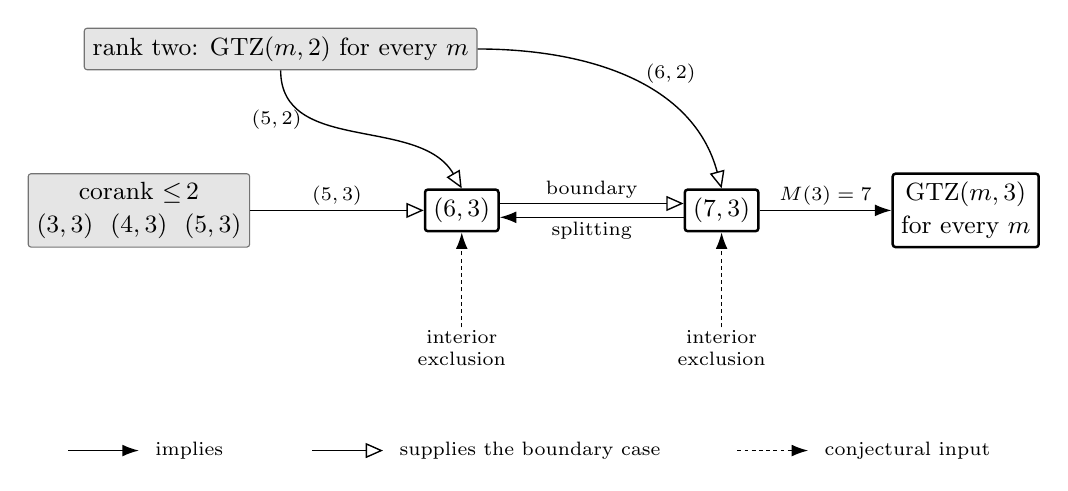
\begin{tikzpicture}[
  x=1cm, y=1cm,
  every node/.style={font=\small, inner sep=3pt},
  proved/.style={draw=black!55, line width=0.4pt, fill=black!10,
                 rounded corners=1pt, align=center},
  openq/.style ={draw=black, line width=0.9pt, fill=white,
                 rounded corners=1pt, align=center},
  hyp/.style   ={font=\scriptsize, align=center, inner sep=1pt},
  tag/.style   ={font=\scriptsize, inner sep=1.5pt},
  imp/.style   ={-{Latex[length=2.1mm,width=1.5mm]}, line width=0.5pt},
  bnd/.style   ={-{Triangle[open,length=2.2mm,width=1.9mm]}, line width=0.5pt},
  cnj/.style   ={-{Latex[length=2.1mm,width=1.5mm]}, line width=0.5pt,
                 dash pattern=on 1.4pt off 1.2pt}]

\node[proved] (two) at (2.7,2.05) {rank two: $\Gtz(m,2)$ for every $m$};
\node[proved] (low) at (0.9,0)    {corank ${\le}\,2$\\[1pt] $(3,3)\ \ (4,3)\ \ (5,3)$};
\node[openq]  (six) at (5.0,0)    {$(6,3)$};
\node[openq]  (sev) at (8.3,0)    {$(7,3)$};
\node[openq]  (all) at (11.4,0)   {$\Gtz(m,3)$\\[1pt] for every $m$};

\node[hyp] (h6) at (5.0,-1.75) {interior\\ exclusion};
\node[hyp] (h7) at (8.3,-1.75) {interior\\ exclusion};

% the boundary analysis at a cell consumes the two cells one size below
\draw[bnd] (low.east) -- node[tag, above] {$(5,3)$} (six.west);
\draw[bnd] (two.south) to[out=-90,in=120]
     node[tag, pos=0.30, left=2pt] {$(5,2)$} (six.north);
\draw[bnd] (two.east) to[out=0,in=105]
     node[tag, pos=0.55, above right=-1pt] {$(6,2)$} (sev.north);
\draw[bnd] ([yshift=2.5pt]six.east) --
     node[tag, above] {boundary} ([yshift=2.5pt]sev.west);

% the logical reductions
\draw[imp] ([yshift=-2.5pt]sev.west) --
     node[tag, below] {splitting} ([yshift=-2.5pt]six.east);
\draw[imp] (sev.east) -- node[tag, above] {$M(3)=7$} (all.west);

\draw[cnj] (h6) -- (six);
\draw[cnj] (h7) -- (sev);

% ---------------------------- legend --------------------------------
\begin{scope}[shift={(0,-3.05)}]
  \draw[imp] (0,0) -- (0.9,0);
  \node[tag, anchor=west] at (1.05,0) {implies};
  \draw[bnd] (3.1,0) -- (4.0,0);
  \node[tag, anchor=west] at (4.15,0) {supplies the boundary case};
  \draw[cnj] (8.5,0) -- (9.4,0);
  \node[tag, anchor=west] at (9.55,0) {conjectural input};
\end{scope}

\end{tikzpicture}

  \caption{Rank three.  Solid arrows are the reductions of
  Corollary~\ref{cor:corank} and Theorem~\ref{thm:window}; the boundary
  analysis of \S\ref{sec:compactness} at a cell consumes the two cells one
  size below.  Dashed arrows carry the two unproved inputs of
  \S\ref{sec:interior}.}
  \label{fig:ladder}
\end{figure}

\section{The equality locus}\label{sec:ties}

The inequality \eqref{eq:dominate} is an equality on a set of full
dimension.  At every size $m\ge k+1$ and every weight vector there is a
design whose best $k$-subset has $\lmin(\SC)=1$, and these designs form
families of dimension $m-1$, the dimension of the weights themselves.  No
argument for $\Gtz$ can therefore carry a margin, and none of the
reductions of \S\ref{sec:real} may consume one.

\subsection{Extremal designs}\label{sec:extremal}

\begin{definition}\label{def:tie}
A design is \emph{extremal} if some $k$-subset dominates and no $k$-subset
dominates strictly: there is a $k$-subset with $\SC\psd I_k$, and no
$k$-subset has $\SC\pd I_k$.
\end{definition}

For a Hermitian matrix $A$, the relation $A\psd I_k$ says
$\lmin(A)\ge1$ and $A\pd I_k$ says $\lmin(A)>1$.

\begin{lemma}\label{lem:tiemax}
A design is extremal if and only if
$\max_{\lvert C\rvert=k}\lmin(\SC)=1$.  At an extremal design every
dominating $k$-subset has $\lmin(\SC)=1$, so that $\SC-I_k$ is
positive semidefinite and singular.
\end{lemma}

\begin{proof}
The maximum is at least $1$ if and only if some $C$ dominates, and exceeds
$1$ if and only if some $C$ dominates strictly.  A dominating $C$ has
$\lmin(\SC)\ge1$, and the maximum being $1$ forces equality.
\end{proof}

For $m\ge k$ put
\begin{equation}\label{eq:alpha}
  \alpha(m,k)\;:=\;\inf_{\dsn}\ \max_{\lvert C\rvert=k}\lmin(\SC),
\end{equation}
the infimum over real designs of size $m$ and rank $k$; this is the real
counterpart of the constant of Remark~\ref{rem:sharpc}, refined by the
size.  By construction $\alpha_k(\R)=\inf_{m\ge k}\alpha(m,k)$, so the
assertion $\alpha_k(\R)\ge1$ of \S\ref{sec:cvalue} is $\Gtz(m,k)$ for
every $m$.  Since a maximum is at least the infimum of maxima,
$\Gtz(m,k)$ holds if and only if $\alpha(m,k)\ge1$, and a design is
extremal exactly when it realizes the value $1$.

At corank zero there is nothing to construct.  If $m=k$ and $k\ge2$ then
the unique $k$-subset is $\{1,\dots,m\}$, and \eqref{eq:coparseval} gives
\[
  \SC-I_k\;=\;\sum_{c}(1-t_c)\,g_c^{\vphantom{\mathsf{H}}}g_c\adj\;\pd\;0 ,
\]
because the $g_c$ are then a basis of $\FF^k$ and $m\ge2$ forces $t_c<1$
for every $c$.  So no design at $m=k$, $k\ge2$, is extremal;
Proposition~\ref{prop:square} computes its value, $1/\max_ct_c$.  Extremal
designs first occur at corank one, where by
Theorem~\ref{thm:corankone}(iii)--(iv) they occur at every weight vector.

\subsection{Splitting, and existence at every size}\label{sec:split}

Evaluating \eqref{eq:dominate} at a vector gives the \emph{gap form}: for
every $k$-subset $C$ and every $x\in\FF^k$,
\begin{equation}\label{eq:gapform}
  x\adj\bigl(\SC-I_k\bigr)x
  \;=\;\sum_{c\in C}\lvert\langle g_c,x\rangle\rvert^{2}
       \;-\;\lVert x\rVert^{2}.
\end{equation}
Neither side involves the weights.

\begin{lemma}\label{lem:parallel}
Let $C$ be a $k$-subset containing two distinct indices $c,c'$ with
$g_{c'}=a\,g_c$ for some scalar $a$.  Then $\SC$ is singular and $C$
does not dominate.
\end{lemma}

\begin{proof}
The family $(g_c)_{c\in C}$ has $k$ members and spans a subspace of
dimension at most $k-1$, so some unit vector $x$ is orthogonal to all of
them.  Then $\SC x=0$, and by \eqref{eq:gapform},
$x\adj(\SC-I_k)x=-1<0$.
\end{proof}

Now let $\dsn$ be a design at $(m,k)$, let $e$ be an index and let
$0<a<t_e$.  Replace the pair $(g_e,t_e)$ by the two pairs $(g_e,a)$ and
$(g_e,t_e-a)$, leaving everything else alone.  The weights remain positive
and still sum to one, and
\[
  a\,g_e^{\vphantom{\mathsf{H}}}g_e\adj+(t_e-a)\,g_e^{\vphantom{\mathsf{H}}}g_e\adj
  \;=\;t_e\,g_e^{\vphantom{\mathsf{H}}}g_e\adj,
\]
so \eqref{eq:parseval} is unchanged and the result is a design at
$(m+1,k)$.  The vector is not rescaled: \eqref{eq:parseval} is affected
only through the total weight carried by a direction.  This is the
\emph{split} at $e$ with ratio $a$.

Iterating splits from a design at $(k+1,k)$ produces, at size $m$, a
design whose $m$ vectors take at most $k+1$ distinct values and whose
weights are arbitrary subject to prescribed class totals.  We construct
these directly.

\begin{theorem}[Lean]\label{thm:tieseverywhere}
Let $k\ge1$ and $m\ge k+1$, let $t$ be a weight vector on $m$ atoms, and
let $\varphi:\{1,\dots,m\}\to\{1,\dots,k+1\}$ be a surjection.  Put
\[
  T_j\;:=\;\sum_{\varphi(c)=j}t_c \qquad (1\le j\le k+1),
\]
let $(h_j,T_j)_{j\le k+1}$ be a design at $(k+1,k)$ with weights $T$ in
which every $k$-subset dominates and none dominates strictly, and set
$g_c:=h_{\varphi(c)}$.  Then $(g_c,t_c)_{c\le m}$ is an extremal design at
$(m,k)$ with weights exactly $t$.  In particular extremal designs exist at
$(m,k)$ for every $m\ge k+1$, over either field, and at every weight
vector.
\end{theorem}

\begin{proof}
The $T_j$ are positive and sum to one, so Theorem~\ref{thm:corankone}(iii)--(iv)
supplies the design $(h_j,T_j)$ demanded.  Grouping the sum
\eqref{eq:parseval} by classes,
\[
  \sum_{c=1}^{m}t_c\,g_c^{\vphantom{\mathsf{H}}}g_c\adj
  \;=\;\sum_{j=1}^{k+1}\Bigl(\sum_{\varphi(c)=j}t_c\Bigr)
        h_j^{\vphantom{\mathsf{H}}}h_j\adj
  \;=\;\sum_{j=1}^{k+1}T_j\,h_j^{\vphantom{\mathsf{H}}}h_j\adj\;=\;I_k,
\]
so $(g,t)$ is a design at $(m,k)$, with weights $t$ by construction.

Let $C$ be a $k$-subset.  If $\varphi$ is not injective on $C$ then $C$
carries two equal vectors and does not dominate, by
Lemma~\ref{lem:parallel}.  If $\varphi$ is injective on $C$ then
$\varphi(C)$ is a $k$-subset of $\{1,\dots,k+1\}$ and
\[
  \SC\;=\;\sum_{c\in C}h_{\varphi(c)}^{\vphantom{\mathsf{H}}}h_{\varphi(c)}\adj
      \;=\;S_{\varphi(C)},
\]
which dominates and does not dominate strictly.  Since $\varphi$ is
surjective there is at least one $C$ of the second kind: choose $k$ of the
$k+1$ classes and one index from each.  Hence some $k$-subset dominates
and none dominates strictly.
\end{proof}

At $m=k+1$ the surjection is a bijection and the theorem returns
Theorem~\ref{thm:corankone}(iii)--(iv).  At $m\ge k+2$ some class contains two indices,
so the design carries a pair of equal vectors; \S\ref{sec:diamond} shows
that this feature is not forced.

\begin{proposition}\label{prop:section}
For fixed $\varphi$ the assignment $t\mapsto \dsn(t,\varphi)$ of
Theorem~\ref{thm:tieseverywhere} is a section of the weight map over the
whole open simplex: every weight vector carries an extremal design.  At
$m=k+1$ it is onto, in the following sense: two extremal designs of size
$k+1$ with the same weights differ by
\[
  g_c\;\longmapsto\;\varepsilon_c\,Ug_c,
  \qquad U\in O(k)\ \text{resp.}\ U(k),\qquad
  \lvert\varepsilon_c\rvert=1 ,
\]
a transformation under which every $\SC$ becomes $U\SC U\adj$, so that no
$\lmin(\SC)$ changes and neither domination nor extremality is
affected.  Consequently the extremal
locus at corank one has dimension $m-1=k$ modulo that group, and
at every $m\ge k+1$ the extremal locus contains, for each partition of
$\{1,\dots,m\}$ into $k+1$ nonempty blocks, a family of dimension $m-1$.
\end{proposition}

\begin{proof}
Only the corank-one assertion needs an argument.  Let $m=k+1$.  By
Theorem~\ref{thm:corankone} a design of that size with weights $t$ is
extremal if and only if its chart projection is $P=I-zz\adj$ with
$\lvert z_c\rvert^{2}=(1-t_c)/k$ for every $c$.  One direction is part
(iii) of that theorem.  For the other, extremality forbids strict
domination, so by part (i) no $p_{c_0}$ exceeds the $t$-mean
$\sum_ct_cp_c$; the weights being positive, a family none of whose members
exceeds its own weighted mean is constant, and by \eqref{eq:pnorm} the
constant is $1/k$, which is the stated condition on $z$.  These moduli
determine $z$ up to the individual phases $\varepsilon_c$, and $P$
determines $V$ up to $V\mapsto VU$, since two isometries with the same
range differ by the unitary $U=V\adj V'$.  Replacing $z$ by
$\diag(\varepsilon)z$ replaces $P$ by
$\diag(\varepsilon)P\diag(\varepsilon)\adj$, the identity term surviving
that conjugation because $\lvert\varepsilon_c\rvert=1$; so $V$ becomes
$\diag(\varepsilon)V$ and $g_c=v_c/\sqrt{t_c}$ becomes $\varepsilon_cg_c$,
under which $g_c^{\vphantom{\mathsf{H}}}g_c\adj$ is unchanged.  The fibre of
the weight map over each $t$ is therefore a single orbit, the
quotient is mapped bijectively onto the open simplex, and the dimension is
$m-1=k$.
\end{proof}

The corank-one classification does not extend: the equations
\eqref{eq:tielaw} that cut it out have no solutions above corank one.

\begin{proposition}[Lean]\label{prop:tielawcorank}
Let $k\ge2$.  If a design of size $m$ satisfies $k\,t_c\ell_c=k-1+t_c$ at
every atom, then $m=k+1$.
\end{proposition}

\begin{proof}
Sum \eqref{eq:tielaw} over $c$.  The left side is
$k\sum_ct_c\ell_c=k^{2}$ by Lemma~\ref{lem:trace}; the right side is
$m(k-1)+\sum_ct_c=m(k-1)+1$.  Hence $(k-1)(k+1)=m(k-1)$, and $k\ge2$
permits the cancellation.
\end{proof}

So above corank one the extremal designs are cut out by no such closed
system.  The designs of Theorem~\ref{thm:tieseverywhere} satisfy
\eqref{eq:tielaw} at an atom $c$ precisely when $c$ is alone in its class:
substituting $\ell_c=(k-1+T_{\varphi(c)})/(kT_{\varphi(c)})$, which is
Theorem~\ref{thm:corankone}(iii) read at the class totals, into
\eqref{eq:tielaw} cancels the products and leaves
$t_c(k-1)=T_{\varphi(c)}(k-1)$, that is $t_c=T_{\varphi(c)}$.  The law
therefore fails at exactly the atoms of the classes that carry more than
one, and at $m=k+2$ it fails at two atoms out of $k+2$.  The following
instances are used again in \S\ref{sec:interior} and in
Appendix~\ref{app:data}.

\begin{example}[Lean]\label{ex:split}
Take for $(h_j)$ the regular tetrahedron of Example~\ref{ex:tetra}, so
that $k=3$, $T_j=\tfrac14$, $\ell(h_j)=3$ and
$\langle h_i,h_j\rangle=-1$ for $i\ne j$.

At $m=6$, with $\varphi=(1,2,3,3,4,4)$ and weights
$\bigl(\tfrac14,\tfrac14,a,\tfrac14-a,b,\tfrac14-b\bigr)$ for any
$0<a,b<\tfrac14$, Theorem~\ref{thm:tieseverywhere} produces a
two-parameter family of extremal designs at $(6,3)$.  Every leverage is
$3$, while \eqref{eq:tielaw} at $k=3$ reads $9t_c=2+t_c$, that is
$t_c=\tfrac14$: the law fails at each of the four split atoms, in
accordance with Proposition~\ref{prop:tielawcorank}.

At $m=7$, with $\varphi=(1,2,3,4,1,2,3)$ and weights
$\bigl(\tfrac18,\tfrac18,\tfrac18,\tfrac14,\tfrac18,\tfrac18,
\tfrac18\bigr)$, one obtains an extremal design at $(7,3)$ in which again
every leverage is $3$.  Of its $35$ triples, the $20$ carrying three
distinct classes dominate: for such a triple $T$, missing the class $j$,
the computation of Example~\ref{ex:tetra} gives
\[
  S_T\;=\;4I_3-h_j^{\vphantom{\mathsf{T}}}h_j\tp,
  \qquad
  x\tp(S_T-I_3)x\;=\;3\lVert x\rVert^{2}-\langle h_j,x\rangle^{2},
\]
so that the gap has spectrum $\{0,3,3\}$ and $\lmin(S_T)=1$.  The
remaining $15$ triples repeat a class and do not dominate, by
Lemma~\ref{lem:parallel}.
\end{example}

\subsection{No margin}\label{sec:nomargin}

\begin{corollary}[Lean]\label{cor:nomargin}
Let $k\ge1$, $m\ge k+1$ and $\varepsilon>0$.  For every weight vector $t$
there is a design at $(m,k)$ with weights $t$ admitting no $k$-subset with
$\SC\psd(1+\varepsilon)I_k$.  Consequently $\alpha(m,k)\le1$, and if
$\Gtz(m,k)$ holds then $\alpha(m,k)=1$ and the infimum in
\eqref{eq:alpha} is attained.
\end{corollary}

\begin{proof}
Let $\dsn$ be the extremal design of Theorem~\ref{thm:tieseverywhere} with
weights $t$.  If some $k$-subset had $\SC\psd(1+\varepsilon)I_k$ then
$\SC-I_k\psd\varepsilon I_k\pd0$, so that $C$ would dominate strictly.
The remaining assertions are Lemma~\ref{lem:tiemax}.
\end{proof}

There is no uniform margin.  For every $\varepsilon>0$ the assertion
``every design admits a $k$-subset with $\SC\psd(1+\varepsilon)I_k$'' is
false, at every cell with $m\ge k+1$.  An argument whose output is a
strict inequality --- a positivity certificate carrying a strictly
positive multiplier, or a bound $\lmin(\SC)\ge1+f$ with $f$ a positive
function of the design data --- therefore fails at the extremal designs
themselves, whatever its degree or complexity.

There is no slack to transport.  Suppose $\Gtz(m,k)$ is derived from a
smaller cell $(m',k')$ with $m'\ge k'+1$.  The slack
$\max_C\lmin(\SC)-1$ available at the smaller cell is zero at the designs
of Theorem~\ref{thm:tieseverywhere}, so no step may consume a positive
amount of it: the reduction must be an identity and not an estimate.  The
compression lift of \S\ref{sec:boundary} is such an identity at vanishing
weight, and Theorem~\ref{thm:sharp} exhibits its failure at every positive
weight, on the extremal locus itself.

The locus has full dimension.  By
Proposition~\ref{prop:section} the extremal locus meets every point of the
open weight simplex, at every size $m\ge k+1$, and has dimension $m-1$,
which is the dimension of the weights.  No restriction on the weights
avoids it, and no compactness argument on a subregion of the design space
yields a positive infimum for the slack unless the closure of that
subregion misses the locus.  The analysis at the extremal points must
therefore be first-order, and \S\ref{sec:compactness} and
\S\ref{sec:interior} supply it.  Appendix~\ref{app:graveyard} collects
the strategies that fail for these reasons, together with their refuting
witnesses.  Figure~\ref{fig:section} draws the locus at $(6,3)$.

\begin{figure}[ht]
  \centering
  % The equality locus of section sec:ties as a section of the weight map, at
% (m,k) = (6,3).  Orthographic projection of R^3 with azimuth 20 and elevation
% 15 degrees, scaled by 1.35cm:
%   X = 1.35(-0.3420 x_1 + 0.9397 x_2)
%   Y = 1.35(-0.2432 x_1 - 0.0885 x_2 + 0.9659 x_3)
% so one unit of height x_3 lifts a point by 1.35*0.9659 = 1.3040cm.
%
% FLOOR.  The base drawn is the two-dimensional slice t_4=t_5=t_6=1/6 of the
% open weight simplex at m=6; on it t_1+t_2+t_3=1/2, and the barycentric
% coordinate u=2(t_1,t_2,t_3) carries the slice to the equilateral triangle of
% circumradius 2.8 in the plane x_3=0,
%   V1 = ( 2.8, 0.0000, 0),  V2 = (-1.4, 2.4249, 0),  V3 = (-1.4,-2.4249, 0),
% the uniform weight vector t_c=1/6 landing on the centroid u=(1/3,1/3,1/3).
% Every coordinate below is u_1 V1 + u_2 V2 + u_3 V3 projected and then raised
% by 1.3040 z, with u and z in the trailing comment.
%
% SHEETS.  The fibre of the weight map is drawn as one vertical dimension and
% the three heights carry no numerical meaning.  Sheet j is the graph of
%   z = z0 + a q(u),   q(u) = u_1u_2 + u_2u_3 + u_3u_1,
%   (z0,a) = (1.60, 0.30), (3.05,-0.28), (4.50, 0.32),
% and q is 0 at the corners, 1/4 at the edge midpoints, 1/3 at the centroid.
% Each boundary edge is the quadratic Bezier through the corner, edge-midpoint
% and corner heights, written as the equal cubic: its two control points sit at
% the thirds of the chord, raised by 4d/3, where d = 1.3040 a/4 is the height of
% the edge midpoint above the chord midpoint,
%   d    = 0.0978, -0.0913, 0.1043,
%   4d/3 = 0.1304, -0.1217, 0.1391.
%
% A dashed boundary marks exclusion.  The simplex is open, and so is each sheet
% over it.  The subregion is the parallelogram of barycentric half-widths 0.05
% about u = (.36,.16,.48), drawn on the floor and on each of the three sheets.
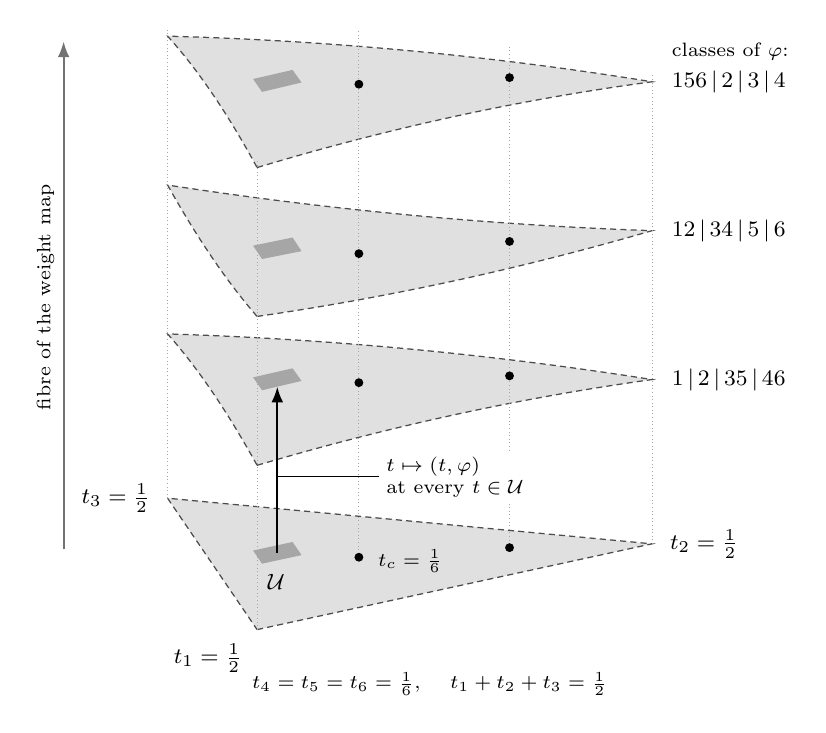
\begin{tikzpicture}[
  x=1cm, y=1cm,
  vec/.style={-{Latex[length=2mm,width=1.5mm]}, line width=0.75pt},
  open/.style={draw=black!70, line width=0.45pt, dashed,
               dash pattern=on 2.2pt off 1.5pt},
  frame/.style={draw=black!35, line width=0.3pt, densely dotted},
  every node/.style={font=\small}]

% ---- the floor: the slice of the open weight simplex --------------------
\filldraw[fill=black!12, open]
  (-1.2928,-0.9193) --                              % u = (1,0,0)
  ( 3.7226, 0.1699) --                              % u = (0,1,0)
  (-2.4297, 0.7494) -- cycle;                       % u = (0,0,1)
\path[fill=black!35]
  (-0.8421, 0.1938) --                              % u = (.26,.21,.53)
  (-0.7284, 0.0270) --                              % u = (.36,.21,.43)
  (-1.2300,-0.0819) --                              % u = (.46,.11,.43)
  (-1.3437, 0.0849) -- cycle;                       % u = (.36,.11,.53)

% ---- sheet 1: the classes 1 | 2 | 35 | 46 -------------------------------
\filldraw[fill=black!12, open]
  (-1.2928,1.1671)                                  % u = (1,0,0), z = 1.60
    .. controls ( 0.3790,1.6606) and ( 2.0508,2.0236) ..
  ( 3.7226,2.2563)                                  % u = (0,1,0), z = 1.60
    .. controls ( 1.6718,2.5799) and (-0.3789,2.7730) ..
  (-2.4297,2.8358)                                  % u = (0,0,1), z = 1.60
    .. controls (-2.0507,2.4100) and (-1.6718,1.8537) .. cycle;
\path[fill=black!35]
  (-0.8421,2.3990) --                               % z = 1.6911
  (-0.7284,2.2389) --                               % z = 1.6962
  (-1.2300,2.1202) --                               % z = 1.6887
  (-1.3437,2.2842) -- cycle;                        % z = 1.6866

% ---- sheet 2: the classes 12 | 34 | 5 | 6 -------------------------------
\filldraw[fill=black!12, open]
  (-1.2928,3.0579)                                  % u = (1,0,0), z = 3.05
    .. controls ( 0.3790,3.2993) and ( 2.0508,3.6623) ..
  ( 3.7226,4.1471)                                  % u = (0,1,0), z = 3.05
    .. controls ( 1.6718,4.2186) and (-0.3789,4.4117) ..
  (-2.4297,4.7266)                                  % u = (0,0,1), z = 3.05
    .. controls (-2.0507,4.0487) and (-1.6718,3.4924) .. cycle;
\path[fill=black!35]
  (-0.8421,4.0601) --                               % z = 2.9650
  (-0.7284,3.8871) --                               % z = 2.9602
  (-1.2300,3.7873) --                               % z = 2.9672
  (-1.3437,3.9567) -- cycle;                        % z = 2.9692

% ---- sheet 3: the classes 156 | 2 | 3 | 4 -------------------------------
\filldraw[fill=black!12, open]
  (-1.2928,4.9487)                                  % u = (1,0,0), z = 4.50
    .. controls ( 0.3790,5.4509) and ( 2.0508,5.8139) ..
  ( 3.7226,6.0379)                                  % u = (0,1,0), z = 4.50
    .. controls ( 1.6718,6.3702) and (-0.3789,6.5633) ..
  (-2.4297,6.6174)                                  % u = (0,0,1), z = 4.50
    .. controls (-2.0507,6.2003) and (-1.6718,5.6440) .. cycle;
\path[fill=black!35]
  (-0.8421,6.1885) --                               % z = 4.5972
  (-0.7284,6.0288) --                               % z = 4.6026
  (-1.2300,5.9095) --                               % z = 4.5946
  (-1.3437,6.0734) -- cycle;                        % z = 4.5924

% ---- the fibre direction: three corner walls and two whole fibres -------
\draw[frame] (-1.2928,-0.9193) -- (-1.2928,5.05);
\draw[frame] ( 3.7226, 0.1699) -- ( 3.7226,6.14);
\draw[frame] (-2.4297, 0.7494) -- (-2.4297,6.72);
\draw[frame] ( 0.0000, 0.0000) -- ( 0.0000,6.70);   % u = (1/3,1/3,1/3)
\draw[frame] ( 1.9130, 0.1217) -- ( 1.9130,6.50);   % u = (.14,.68,.18)

% ---- the design each fibre meets on each sheet --------------------------
\fill ( 0.0000,0.0000) circle (1.6pt);
\fill ( 0.0000,2.2168) circle (1.6pt);              % z = 1.7000
\fill ( 0.0000,3.8555) circle (1.6pt);              % z = 2.9567
\fill ( 0.0000,6.0071) circle (1.6pt);              % z = 4.6067
\fill ( 1.9130,0.1217) circle (1.6pt);
\fill ( 1.9130,2.3031) circle (1.6pt);              % z = 1.6728
\fill ( 1.9130,4.0102) circle (1.6pt);              % z = 2.9820
\fill ( 1.9130,6.0910) circle (1.6pt);              % z = 4.5777

% ---- the section over the subregion -------------------------------------
\draw[vec] (-1.0361,0.0560) -- (-1.0361,2.1661);    % u = (.36,.16,.48)
\draw[line width=0.3pt] (-1.0361,1.02) -- (0.25,1.02);
\node[anchor=west, font=\scriptsize, align=left, fill=white, inner sep=1.5pt]
  at (0.29,1.02) {$t\mapsto\dsn(t,\varphi)$\\ at every $t\in\mathcal{U}$};
\node[anchor=north, font=\footnotesize] at (-1.05,-0.09) {$\mathcal{U}$};

% ---- the base, labelled -------------------------------------------------
\node[anchor=north east, font=\footnotesize] at (-1.36,-0.98) {$t_1=\tfrac12$};
\node[anchor=west,       font=\footnotesize] at ( 3.83,0.1699) {$t_2=\tfrac12$};
\node[anchor=east,       font=\footnotesize] at (-2.53,0.7494) {$t_3=\tfrac12$};
\node[anchor=west,  font=\scriptsize] at (0.12,-0.05) {$t_c=\tfrac16$};
\node[anchor=north, font=\scriptsize] at (0.90,-1.34)
  {$t_4=t_5=t_6=\tfrac16$, \quad $t_1+t_2+t_3=\tfrac12$};

% ---- the fibre axis and the classes -------------------------------------
\draw[vec, black!55] (-3.75,0.10) -- (-3.75,6.55);
\node[rotate=90, font=\scriptsize] at (-3.98,3.30) {fibre of the weight map};
\node[anchor=west, font=\scriptsize]   at (3.85,6.42) {classes of $\varphi$:};
\node[anchor=west, font=\footnotesize] at (3.85,6.0379) {$156\,|\,2\,|\,3\,|\,4$};
\node[anchor=west, font=\footnotesize] at (3.85,4.1471) {$12\,|\,34\,|\,5\,|\,6$};
\node[anchor=west, font=\footnotesize] at (3.85,2.2563) {$1\,|\,2\,|\,35\,|\,46$};

\end{tikzpicture}

  \caption{The equality locus as a section, at $(6,3)$.  Floor: the slice
  $t_4=t_5=t_6=\tfrac16$ of the open weight simplex, its excluded boundary
  dashed and the uniform point marked.  Vertical: the fibre of the weight
  map, drawn as a single dimension.  Each sheet is a section
  $t\mapsto\dsn(t,\varphi)$ of Proposition~\ref{prop:section} restricted to
  that slice; the section is defined at every weight vector and its image has
  dimension $m-1=5$, the dimension of the weights.  One sheet occurs for each
  partition of $\{1,\dots,6\}$ into four classes, $65$ in all, of which three
  are drawn.  However small, the shaded $\mathcal{U}$ meets every one of them,
  so no restriction of the weights isolates a region on which the slack has a
  positive infimum; four of the nine strategies of
  Appendix~\ref{app:graveyard} fail on that account.}
  \label{fig:section}
\end{figure}

\subsection{The diamond}\label{sec:diamond}

Every design of Theorem~\ref{thm:tieseverywhere} of size $m\ge k+2$
carries a pair of equal vectors and takes at most $k+1$ distinct
values; neither feature is forced.  We exhibit an extremal design at
$(5,3)$ whose five vectors are pairwise non-parallel.  It is described
by a graph, and its data are rational even though its vectors are not.

Let $\gph$ be the complete graph on the vertices $1,2,3,4$ with the edge
$34$ deleted, grounded at the vertex $4$, and list its five edges as
\[
  e_0=12,\qquad e_1=13,\qquad e_2=14,\qquad e_3=23,\qquad e_4=24 .
\]
A potential is a vector $y=(y_1,y_2,y_3)\in\R^3$, the ground carrying
$y_4=0$, and the \emph{drop} across an edge is the difference of the
potentials at its endpoints:
\begin{equation}\label{eq:drops}
  d(y)\;=\;\bigl(y_1-y_2,\ y_1-y_3,\ y_1,\ y_2-y_3,\ y_2\bigr)
  \;=\;\bigl(\langle b_e,y\rangle\bigr)_{0\le e\le4},
\end{equation}
the reduced incidence vectors being
\[
  b_0=(1,-1,0),\quad b_1=(1,0,-1),\quad b_2=(1,0,0),\quad
  b_3=(0,1,-1),\quad b_4=(0,1,0).
\]
Give the edges the conductances and weights
\[
  c\;=\;(2,3,3,3,3), \qquad t_e\;=\;\tfrac15\quad(0\le e\le4),
\]
and form the weighted Laplacian
\begin{equation}\label{eq:laplacian}
  L\;:=\;\sum_{e=0}^{4}c_e\,b_e^{\vphantom{\mathsf{T}}}b_e\tp
  \;=\;\begin{pmatrix} 8&-2&-3\\ -2&8&-3\\ -3&-3&6\end{pmatrix},
  \qquad
  y\tp Ly\;=\;\sum_{e}c_e\,d_e(y)^{2}.
\end{equation}
Its leading principal minors are $8$, $60$ and $\det L=180$, so $L\pd0$.
Choose any $R$ with $R\tp LR=I_3$ --- for instance $R=L^{-1/2}$ --- and
put
\begin{equation}\label{eq:diamondatoms}
  g_e\;:=\;\sqrt{5c_e}\;R\tp b_e \qquad (0\le e\le 4).
\end{equation}
Then
\[
  \sum_{e}t_e\,g_e^{\vphantom{\mathsf{T}}}g_e\tp
  \;=\;\sum_e \tfrac15\cdot 5c_e\,R\tp b_e^{\vphantom{\mathsf{T}}}b_e\tp R
  \;=\;R\tp LR\;=\;I_3,
\]
so $(g_e,t_e)$ is a design at $(5,3)$; call it $\dsn_{\Diamond}$.  It is
determined by the graph data up to the ambiguity $R\mapsto RU$ with $U$
orthogonal, which replaces every $g_e$ by $U\tp g_e$ and every $\SC$ by
$U\tp\SC U$, changing no $\lmin(\SC)$.

Since $RR\tp=L^{-1}$,
\begin{equation}\label{eq:diamondlev}
  \ell_e\;=\;5c_e\,b_e\tp L^{-1}b_e ,
  \qquad
  L^{-1}\;=\;\frac1{180}
  \begin{pmatrix}39&21&30\\ 21&39&30\\ 30&30&60\end{pmatrix},
\end{equation}
whence $b_0\tp L^{-1}b_0=\tfrac{36}{180}=\tfrac15$ and
$b_e\tp L^{-1}b_e=\tfrac{39}{180}=\tfrac{13}{60}$ for $e\ge1$, so that
\[
  \ell_0=2,\qquad \ell_1=\ell_2=\ell_3=\ell_4=\tfrac{13}4 .
\]
As a check, $\sum_et_e\ell_e=\tfrac15\bigl(2+4\cdot\tfrac{13}4\bigr)=3=k$,
as Lemma~\ref{lem:trace} requires.  The substitution $y=Rx$, a bijection
of $\R^3$, gives for every $3$-subset $C$
\[
  x\tp\SC x=\sum_{e\in C}5c_e\,d_e(y)^{2},
  \qquad
  x\tp x=x\tp R\tp LRx=\sum_{e}c_e\,d_e(y)^{2},
\]
so that domination becomes a statement about potentials alone, free of
the whitening $R$:
\begin{equation}\label{eq:diamondgap}
  x\tp\bigl(\SC-I_3\bigr)x\;=\;Q_C(y),
  \qquad
  Q_C(y):=\sum_{e=0}^{4}\bigl(5\cdot[e\in C]-1\bigr)c_e\,d_e(y)^{2},
\end{equation}
where $[\,\cdot\,]$ is $1$ when the enclosed statement holds and $0$
otherwise; and $C$ dominates if and only if $Q_C\ge0$ on $\R^3$, and
dominates strictly if and only if $Q_C>0$ off the origin.

\begin{example}[Lean]\label{ex:diamond}
The design $\dsn_{\Diamond}$ is extremal at $(5,3)$; its five vectors are
pairwise non-parallel; and it is not one of the designs of
Theorem~\ref{thm:tieseverywhere}.
\end{example}

\begin{proof}
For the star at the vertex $1$, that is $C=\{e_0,e_1,e_2\}$, expanding
\eqref{eq:diamondgap} by means of \eqref{eq:drops} gives
\begin{align*}
  Q_C(y)&=8(y_1-y_2)^2+12(y_1-y_3)^2+12y_1^2-3(y_2-y_3)^2-3y_2^2\\
        &=32y_1^2+2y_2^2+9y_3^2-16y_1y_2-24y_1y_3+6y_2y_3 .
\end{align*}
Doubling and completing the square in $y_1$ leaves $9y_3^{2}$:
\begin{equation}\label{eq:diamondstar}
  2\,Q_C(y)\;=\;\bigl(8y_1-2y_2-3y_3\bigr)^{2}+9\,y_3^{2} .
\end{equation}
So $C$ dominates.  The right side vanishes at the nonzero $y=(1,4,0)$, so
$Q_C$ is singular and $C$ does not dominate strictly.

There are ten $3$-subsets: eight spanning trees of $\gph$, and its two
triangles $\{e_0,e_1,e_3\}$ on the vertices $1,2,3$ and
$\{e_0,e_2,e_4\}$ on $1,2,4$.  For each, the potential listed below gives
the stated value of $Q_C$:
\[
\begin{array}{llr@{\qquad}llr}
\{e_0,e_1,e_2\} & (1,4,0)  & 0 &
\{e_0,e_1,e_3\} & (1,1,1)  & -6\\
\{e_0,e_1,e_4\} & (4,1,5)  & 0 &
\{e_0,e_2,e_3\} & (1,4,5)  & 0\\
\{e_0,e_2,e_4\} & (0,0,1)  & -6 &
\{e_0,e_3,e_4\} & (4,1,0)  & 0\\
\{e_1,e_2,e_3\} & (2,8,5)  & 0 &
\{e_1,e_2,e_4\} & (3,-3,5) & 0\\
\{e_1,e_3,e_4\} & (8,2,5)  & 0 &
\{e_2,e_3,e_4\} & (-3,3,5) & 0
\end{array}
\]
Each entry is one evaluation of \eqref{eq:diamondgap}.  At
$\{e_1,e_2,e_4\}$ and $y=(3,-3,5)$, for instance, the drops
\eqref{eq:drops} are $(6,-2,3,-8,-3)$ and
\[
  Q_C(y)=-2\cdot36+12\cdot4+12\cdot9-3\cdot64+12\cdot9=0 .
\]
For each triangle the potential is constant on the triangle's vertex set,
so its three drops vanish and $Q_C$ reduces to minus the Dirichlet
contribution of the two edges leaving that set.  Each of those two carries
conductance $3$ and a drop of modulus $1$, so $Q_C=-6$.  Hence no
$3$-subset has $Q_C>0$ off the origin, that is none dominates strictly,
while by the first paragraph one dominates: $\dsn_{\Diamond}$ is extremal.

Proportionality of $g_e$ and $g_f$ is proportionality of $b_e$ and $b_f$,
since $R\tp$ is invertible and the factors $\sqrt{5c_e}$ do not
vanish.  Proportional nonzero vectors have equal support, and the five
supports $\{1,2\},\{1,3\},\{1\},\{2,3\},\{2\}$ are distinct.  So no two
vectors are parallel; in particular $\dsn_{\Diamond}$ carries five distinct
directions, whereas a design of Theorem~\ref{thm:tieseverywhere} carries
at most $k+1=4$.
\end{proof}

\begin{corollary}[Lean]\label{cor:noparallel}
The assertion ``every extremal design contains two parallel vectors'' is
true for every design of Theorem~\ref{thm:tieseverywhere} of size
$m\ge k+2$, and false at $(5,3)$.
\end{corollary}

\begin{proof}
If $m\ge k+2$ then $\varphi$ is not injective, so two indices carry equal
vectors.  Example~\ref{ex:diamond} is the counterexample.
\end{proof}

An argument branching on the presence of a parallel pair therefore
requires a separate treatment of $\dsn_{\Diamond}$, and of every extremal
design not obtained by splitting a smaller one.  Whether the tetrahedron
and the diamond generate the whole rank-three extremal locus is
Problem~\ref{prob:structure}.  Figure~\ref{fig:diamond} shows the graph
and its incidence vectors.

\begin{figure}[ht]
  \centering
  % Left: the graph Gamma = K_4 minus the edge 34, grounded at the vertex 4;
% the line weight of an edge is proportional to its conductance.
% Right: the five reduced incidence vectors, drawn in R^3 by the orthographic
% projection with azimuth 20 and elevation -28 degrees, scaled by 1.5cm:
%   X = 1.5(-0.3420 y_1 + 0.9397 y_2)
%   Y = 1.5( 0.4411 y_1 + 0.1606 y_2 + 0.8830 y_3)
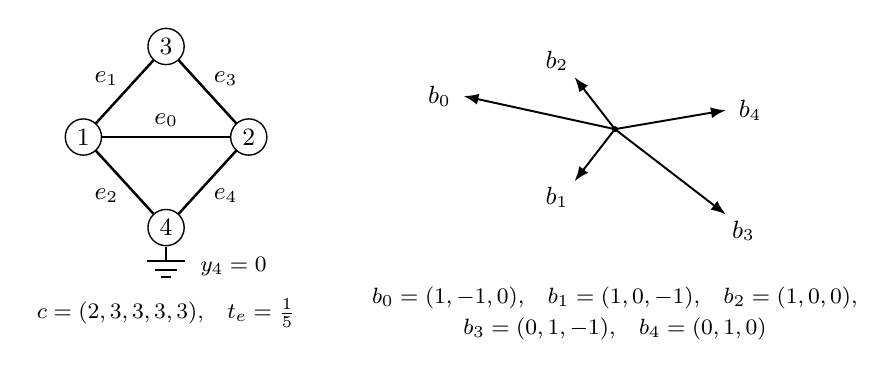
\begin{tikzpicture}[
  x=1cm, y=1cm,
  ver/.style={circle, draw, line width=0.5pt, fill=white, inner sep=0pt,
              minimum size=4.6mm, font=\small},
  spine/.style={line width=0.6pt},
  rim/.style={line width=0.9pt},
  vec/.style={-{Latex[length=1.9mm,width=1.4mm]}, line width=0.7pt},
  every node/.style={font=\small}]

% ================= the graph =============================================
\begin{scope}
  \coordinate (v1) at (-1.05, 0);
  \coordinate (v2) at ( 1.05, 0);
  \coordinate (v3) at ( 0, 1.15);
  \coordinate (v4) at ( 0,-1.15);

  \draw[rim]   (v1)--(v3) node[midway, above left=-2pt]  {$e_1$};
  \draw[rim]   (v2)--(v3) node[midway, above right=-2pt] {$e_3$};
  \draw[rim]   (v1)--(v4) node[midway, below left=-2pt]  {$e_2$};
  \draw[rim]   (v2)--(v4) node[midway, below right=-2pt] {$e_4$};
  \draw[spine] (v1)--(v2) node[midway, above] {$e_0$};

  \node[ver] at (v1) {$1$};
  \node[ver] at (v2) {$2$};
  \node[ver] at (v3) {$3$};
  \node[ver] at (v4) {$4$};

  % the ground
  \draw[line width=0.5pt] (0,-1.40)--(0,-1.58);
  \draw[line width=0.7pt] (-0.24,-1.58)--(0.24,-1.58);
  \draw[line width=0.5pt] (-0.14,-1.69)--(0.14,-1.69);
  \draw[line width=0.5pt] (-0.06,-1.78)--(0.06,-1.78);
  \node[anchor=west, font=\footnotesize] at (0.31,-1.64) {$y_4=0$};

  \node[font=\footnotesize] at (0,-2.24)
       {$c=(2,3,3,3,3)$,\quad $t_e=\tfrac15$};
\end{scope}

% ================= the five incidence vectors =============================
\begin{scope}[shift={(5.70,0.10)}]
  \coordinate (O)  at ( 0,0);
  \coordinate (b1) at (-1.9226, 0.4209);   % (1,-1, 0)
  \coordinate (b2) at (-0.5130,-0.6627);   % (1, 0,-1)
  \coordinate (b3) at (-0.5130, 0.6617);   % (1, 0, 0)
  \coordinate (b4) at ( 1.4096,-1.0836);   % (0, 1,-1)
  \coordinate (b5) at ( 1.4096, 0.2408);   % (0, 1, 0)

  \draw[vec] (O)--(b1) node[left=1pt]         {$b_0$};
  \draw[vec] (O)--(b2) node[below left=-2pt]  {$b_1$};
  \draw[vec] (O)--(b3) node[above left=-2pt]  {$b_2$};
  \draw[vec] (O)--(b4) node[below right=-2pt] {$b_3$};
  \draw[vec] (O)--(b5) node[right=1pt]        {$b_4$};
  \fill (O) circle (1.1pt);

  \node[font=\footnotesize, align=center] at (0,-2.34)
    {$b_0=(1,-1,0)$,\quad $b_1=(1,0,-1)$,\quad $b_2=(1,0,0)$,\\[1.5pt]
     $b_3=(0,1,-1)$,\quad $b_4=(0,1,0)$};
\end{scope}

\end{tikzpicture}

  \caption{The diamond $\dsn_{\Diamond}$.  Left: the graph $K_4$ with the edge
  $34$ deleted and the vertex $4$ grounded, its edges carrying the
  conductances $c=(2,3,3,3,3)$ and the uniform weights $t_e=\tfrac15$;
  line weight is proportional to conductance.  Right: the five reduced
  incidence vectors of \eqref{eq:drops}, pairwise non-proportional, whence
  the five atoms \eqref{eq:diamondatoms} are pairwise non-parallel.}
  \label{fig:diamond}
\end{figure}

\subsection{Volume sampling}\label{sec:averaging}

Volume sampling is the probability measure on $k$-subsets adapted to
\eqref{eq:parseval}, and under it the subset sum dominates on average,
clearing the threshold by a factor of at least $k$ in trace.  Turning
that average into a single subset is the derandomization the problem asks
for.

We work
in the chart of \S\ref{sec:chart}: $v_c=\sqrt{t_c}\,g_c$, the matrix $V$
has rows $v_c\adj$ and satisfies $V\adj V=I_k$, and $P=VV\adj$ by
\eqref{eq:chart}.  For a $k$-subset $C$ write $V_C$ for the $k\times k$
submatrix of $V$ on the rows $C$, so that $P[C]=V_C^{\vphantom{\mathsf{H}}}V_C\adj$.

\begin{lemma}\label{lem:cauchybinet}
Let $X$ be $k\times m$ and $Y$ be $m\times k$.  Then
\[
  \det(XY)\;=\;\sum_{\lvert C\rvert=k}
  \det\bigl(X^{C}\bigr)\det\bigl(Y_C\bigr),
\]
where $X^{C}$ is the submatrix of $X$ on the columns $C$ and $Y_C$ the
submatrix of $Y$ on the rows $C$.
\end{lemma}

\begin{proof}
Write $x_1,\dots,x_m$ for the columns of $X$.  The $j$-th column of $XY$
is $\sum_{c}Y_{cj}x_c$, so multilinearity of the determinant in its
columns gives
\[
  \det(XY)\;=\;\sum_{f}\Bigl(\prod_{j=1}^{k}Y_{f(j)j}\Bigr)
  \det\bigl(x_{f(1)},\dots,x_{f(k)}\bigr),
\]
the sum being over all maps $f:\{1,\dots,k\}\to\{1,\dots,m\}$.  A
non-injective $f$ repeats a column and contributes zero.  An injective $f$
has an image $C$ of size $k$; writing $f=\iota_C\circ\sigma$ with
$\iota_C$ the increasing enumeration of $C$ and $\sigma$ a permutation,
the determinant equals $\operatorname{sgn}(\sigma)\det(X^{C})$, and
summing $\operatorname{sgn}(\sigma)\prod_jY_{\iota_C(\sigma(j))j}$ over
$\sigma$ is the Leibniz formula for $\det(Y_C)$.
\end{proof}

Apply the lemma with $X=V\adj$ and $Y=V$.  The columns of $V\adj$ on $C$
are the conjugated rows of $V$ on $C$, so $(V\adj)^{C}=(V_C)\adj$ and each
term is
$\det\bigl((V_C)\adj\bigr)\det(V_C)=\lvert\det V_C\rvert^{2}
=\det\bigl(V_C^{\vphantom{\mathsf{H}}}V_C\adj\bigr)=\det P[C]$, while the left side
is $\det(V\adj V)=1$.  Setting
\begin{equation}\label{eq:dpp}
  \pi_C\;:=\;\det P[C]
  \;=\;\lvert\det V_C\rvert^{2}
  \;=\;\Bigl(\prod_{c\in C}t_c\Bigr)
       \det\Gram\bigl((g_c)_{c\in C}\bigr)
\end{equation}
--- the last equality because $V_C=\diag(\sqrt{t_c})_{c\in C}M_C$ with
$M_C$ the matrix of the selected vectors --- we conclude that $\pi$ is a
probability measure on $k$-subsets, and that $\pi_C>0$ exactly when
$(g_c)_{c\in C}$ is a basis of $\FF^k$.  Call such a $C$ a \emph{basis} of
the design.  The measure $\pi$ is volume sampling \cite{DRVW2006}; it is
the determinantal measure carried by the bases of the underlying matroid
\cite{Lyons2003}.

\begin{lemma}\label{lem:marginal}
For every atom $c$,
\[
  \Pr\nolimits_{\pi}\bigl[c\in C\bigr]\;=\;\sum_{C\ni c}\pi_C
  \;=\;P_{cc}\;=\;s_c .
\]
\end{lemma}

\begin{proof}
Fix $c$ and let $E_\sigma:=\diag(1,\dots,\sigma,\dots,1)$ carry $\sigma$
in the position $c$.  On one hand
$V\adj E_\sigma V=V\adj V+(\sigma-1)v_c^{\vphantom{\mathsf{H}}}v_c\adj$ is a
rank-one perturbation of the identity, and
$\det(I_k+\lambda uu\adj)=1+\lambda\lVert u\rVert^{2}$, so
\[
  \det\bigl(V\adj E_\sigma V\bigr)\;=\;1+(\sigma-1)\lVert v_c\rVert^{2}
  \;=\;1+(\sigma-1)s_c .
\]
On the other hand Lemma~\ref{lem:cauchybinet} applied to
$X=V\adj E_\sigma$ and $Y=V$ gives, since scaling the column $c$ of
$V\adj$ multiplies every minor containing it by that factor,
\[
  \det\bigl(V\adj E_\sigma V\bigr)
  \;=\;\sum_{\lvert C\rvert=k}\sigma^{[c\in C]}\,\pi_C
  \;=\;\sum_{C\not\ni c}\pi_C\;+\;\sigma\sum_{C\ni c}\pi_C .
\]
Both expressions are affine in $\sigma$; comparing the coefficients of
$\sigma$ gives the claim.
\end{proof}

Summing Lemma~\ref{lem:marginal} over $c$ returns $\sum_cs_c=k$
(Lemma~\ref{lem:trace}), the expected cardinality of $C$, as it must.

\begin{theorem}[Lean]\label{thm:leverageaverage}
For every design over either field,
\[
  \sum_{c}s_c\,g_c^{\vphantom{\mathsf{H}}}g_c\adj\;\psd\;I_k .
\]
\end{theorem}

\begin{proof}
Let $x\ne0$; at $x=0$ both sides vanish.  Cauchy--Schwarz at each atom gives
$\lvert\langle g_c,x\rangle\rvert^{2}\le\ell_c\lVert x\rVert^{2}$, whence
\[
  \lVert x\rVert^{2}\sum_c s_c\lvert\langle g_c,x\rangle\rvert^{2}
  \;=\;\sum_c t_c\,\ell_c\lVert x\rVert^{2}\,
        \lvert\langle g_c,x\rangle\rvert^{2}
  \;\ge\;\sum_c t_c\lvert\langle g_c,x\rangle\rvert^{4} .
\]
Cauchy--Schwarz for the probability weights $t$ bounds the right side
below by
\[
  \Bigl(\sum_ct_c\lvert\langle g_c,x\rangle\rvert^{2}\Bigr)^{2}
  \;=\;\lVert x\rVert^{4}
\]
by \eqref{eq:parseval}.  Dividing by
$\lVert x\rVert^{2}>0$ gives
$x\adj\bigl(\sum_cs_cg_c^{\vphantom{\mathsf{H}}}g_c\adj\bigr)x\ge\lVert x\rVert^2$.
\end{proof}

The leverage-weighted sum is the $\pi$-average of the subset sum.

\begin{theorem}\label{thm:average}
For every design over either field,
\[
  \E_{\pi}\bigl[\SC\bigr]
  \;=\;\sum_{c}s_c\,g_c^{\vphantom{\mathsf{H}}}g_c\adj
  \;\psd\;I_k .
\]
\end{theorem}

\begin{proof}
Exchanging the two summations and applying Lemma~\ref{lem:marginal},
\[
  \E_\pi[\SC]\;=\;\sum_{\lvert C\rvert=k}\pi_C\sum_{c\in C}
  g_c^{\vphantom{\mathsf{H}}}g_c\adj
  \;=\;\sum_{c}\Bigl(\sum_{C\ni c}\pi_C\Bigr)g_c^{\vphantom{\mathsf{H}}}g_c\adj
  \;=\;\sum_c s_c\,g_c^{\vphantom{\mathsf{H}}}g_c\adj ,
\]
and the inequality is Theorem~\ref{thm:leverageaverage}.
\end{proof}

The selection problem is thus the derandomization of
Theorem~\ref{thm:average}: the $\pi$-average of $\SC$ dominates, and one
asks for a single $C$.

\begin{proposition}[Lean]\label{prop:jensen}
$\sum_c t_c\ell_c^{2}\ge k^{2}$, with equality if and only if $\ell_c=k$
for every $c$.
\end{proposition}

\begin{proof}
Cauchy--Schwarz for the weights $t$ gives
$\bigl(\sum_ct_c\ell_c\bigr)^{2}\le\sum_ct_c\ell_c^{2}$, and the left side
is $k^{2}$ by Lemma~\ref{lem:trace}.  Equality holds exactly when $\ell$
is constant, and its $t$-mean is $k$.
\end{proof}

Since $\tr\E_\pi[\SC]=\sum_cs_c\ell_c=\sum_ct_c\ell_c^{2}\ge k^{2}$ while
$\tr I_k=k$, the average clears the threshold by a factor at least $k$ in
trace.  No single subset need exceed it: that is
Corollary~\ref{cor:nomargin}.

Averaging characteristic polynomials rather than matrices gives the
mixture
\begin{equation}\label{eq:mixture}
  q(x)\;:=\;\E_\pi\bigl[\chi_{\SC}(x)\bigr]
  \;=\;\sum_{\lvert C\rvert=k}\pi_C\,\det\bigl(xI_k-\SC\bigr).
\end{equation}
Call a basis $C$ \emph{tight} if $1\in\operatorname{spec}\SC$, and a
design \emph{totally tight} if every basis of it is tight.

\begin{proposition}\label{prop:totaltight}
Every design of Theorem~\ref{thm:tieseverywhere} is totally tight.
\end{proposition}

\begin{proof}
Let $C$ be a $k$-subset.  If $\varphi$ is not injective on $C$ then $\SC$
is singular by Lemma~\ref{lem:parallel}, so $\pi_C=0$ by \eqref{eq:dpp}
and $C$ is not a basis.  Otherwise $\SC=S_{\varphi(C)}$ dominates and does
not dominate strictly, so $\lmin(\SC)=1$ by Lemma~\ref{lem:tiemax}.
\end{proof}

\begin{proposition}[Lean]\label{prop:qonezero}
$q(1)=0$ at every totally tight design.
\end{proposition}

\begin{proof}
$q(1)=\sum_C\pi_C\det(I_k-\SC)$, and every summand with $\pi_C>0$ has $C$
a basis, hence tight, hence $\det(I_k-\SC)=0$.
\end{proof}

\begin{proposition}\label{prop:qone}
The mixture \eqref{eq:mixture} is monic of degree $k$; its subleading
coefficient is
\[
  [x^{k-1}]\,q\;=\;-\,\E_\pi\bigl[\tr\SC\bigr]
  \;=\;-\sum_c t_c\ell_c^{2}\;\le\;-k^{2};
\]
and $q(1)=0$ at every totally tight design.
\end{proposition}

\begin{proof}
Each $\chi_{\SC}$ is monic of degree $k$ and $\sum_C\pi_C=1$, so $q$ is
monic of degree $k$; and $[x^{k-1}]\chi_{\SC}=-\tr\SC$, which gives the
first equality.  The second is Lemma~\ref{lem:marginal} again:
\[
  \E_\pi[\tr\SC]=\sum_C\pi_C\sum_{c\in C}\ell_c
  =\sum_c\ell_c\sum_{C\ni c}\pi_C=\sum_cs_c\ell_c=\sum_ct_c\ell_c^{2},
\]
and the bound is Proposition~\ref{prop:jensen}.  The last assertion is
Proposition~\ref{prop:qonezero}.
\end{proof}

We compute the mixture at the tetrahedron of Example~\ref{ex:tetra},
which by Theorem~\ref{thm:corankone}(iii)--(iv) is the corank-one extremal design at
$k=3$ and uniform weights, and is therefore totally tight by
Proposition~\ref{prop:totaltight}.  Each of its four triples has Gram
matrix $4I_3-J$, with $J$ the all-ones matrix, of determinant $16$; so by
\eqref{eq:dpp}
\[
  \pi_C\;=\;\bigl(\tfrac14\bigr)^{3}\cdot16\;=\;\tfrac14
\]
for each of the four, confirming $\sum_C\pi_C=1$ and giving
$\Pr_\pi[c\in C]=3\cdot\tfrac14=\tfrac34=s_c$ as
Lemma~\ref{lem:marginal} requires.  Every triple has spectrum $\{1,4,4\}$,
so every $\chi_{\SC}(x)=(x-1)(x-4)^{2}$ and the mixture is that same
polynomial:
\begin{equation}\label{eq:qtetra}
  q(x)\;=\;(x-1)(x-4)^{2}\;=\;x^{3}-9x^{2}+24x-16 .
\end{equation}
Its subleading coefficient is
$-9=-\sum_ct_c\ell_c^{2}=-4\cdot\tfrac14\cdot9$, so the bound of
Proposition~\ref{prop:jensen} is attained here; $q(1)=0$, as
Proposition~\ref{prop:qone} requires; and the least root of $q$ sits
at the threshold.  Meanwhile
$\E_\pi[\SC]=\tfrac34\sum_cg_c^{\vphantom{\mathsf{T}}}g_c\tp=3I_3$ while
$\max_C\lmin(\SC)=1$: the average clears the threshold by a factor of
three, and no triple exceeds it.

\begin{remark}\label{rem:interlace}
Only the identities above have been used; three nearby statements do
not follow from them.  First, $q$ is not asserted to
be real-rooted; for a projection determinantal measure that is available
through the strong Rayleigh property
\cite{BorceaBrandenLiggett2009,AnariOveisGharan2015}, and nothing here
needs it.  Second, real-rootedness of $q$ would not imply that some $C$
has $\lmin(\SC)$ at least the least root of $q$: the least root of an
average of real-rooted polynomials may exceed the least root of every
member, and an exact two-polynomial witness is recorded in
Appendix~\ref{app:graveyard}.  Third, the hypothesis under which the
conclusion does follow is a common interlacing of the family
$\{\chi_{\SC}:\pi_C>0\}$, equivalently real-rootedness of every convex
combination of it \cite{MSS2015}; that is a property of the family, to be
verified and not inferred, and it fails for the witness just cited.
Establishing it here, and with it the derandomization of
Theorem~\ref{thm:average}, is Problem~\ref{prob:interlace}; by
Proposition~\ref{prop:qone} any such argument is exact at the extremal
designs, where the least root of $q$ is $1$.
\end{remark}

\section{A variational principle}\label{sec:compactness}

A counterexample to $\Gtz(m,k)$ is a design whose selection objective
falls below the threshold.  We would like the worst one, and to read off
what minimality forces.  A worst design need not exist: the space of
designs at a given size and rank is not compact, and a minimizing
sequence need not converge in it (Example~\ref{ex:escape}).

Grant the conjecture at the two cells one size below.  Then a
counterexample at $(m,k)$ may be taken to minimize the chart objective
globally over a compact space, and to have strictly positive weights
(Theorem~\ref{thm:variational}).

The step that discharges the boundary holds at vanishing weight and
fails at every positive weight, however small (Theorem~\ref{thm:sharp}).
It fails on the extremal locus of \S\ref{sec:ties}.  So the argument runs
at the limit point.

\subsection{The compactification}\label{sec:compactchart}

Fix $m$ and $k$.  In a design the weights are confined to the open
simplex and the vectors are not confined.  Parseval controls only the
product: by Lemma~\ref{lem:trace},
\begin{equation}\label{eq:levbound}
  \sum_c s_c\;=\;\sum_c t_c\ell_c\;=\;k,
  \qquad\text{so}\qquad \ell_c\;\le\;\frac{k}{t_c} .
\end{equation}
As a weight tends to zero the corresponding vector may therefore grow
without bound, and it may do so while keeping its leverage score
$s_c=t_c\ell_c$ fixed.

\begin{example}\label{ex:escape}
Let $k=1$, $m=2$ and, for $0<u\le\tfrac12$,
\[
  t_1=1-u,\quad t_2=u,\qquad
  g_1=\frac1{\sqrt{2(1-u)}},\quad g_2=\frac1{\sqrt{2u}} .
\]
Then $t_1g_1^2+t_2g_2^2=\tfrac12+\tfrac12=1$, so this is a design at
$(2,1)$ for every such $u$.  Its leverages are
$\ell_1=\tfrac1{2(1-u)}$ and $\ell_2=\tfrac1{2u}$, and
$\ell_2\to\infty$ as $u\to0$.
No subsequence converges in the design space.  Its leverage scores are
$s_1=s_2=\tfrac12$, constant in $u$.
\end{example}

The chart of \S\ref{sec:chart} is the change of variables that
retains the leverage scores and discards the divergence.  With
$v_c=\sqrt{t_c}\,g_c$ and $P=VV\adj$ as in \eqref{eq:chart},
\begin{equation}\label{eq:pivotlev}
  P_{cc}\;=\;\lVert v_c\rVert^2\;=\;t_c\ell_c\;=\;s_c ,
\end{equation}
so the divergence in \eqref{eq:levbound} sits entirely in the factor
$1/t_c$: what the chart records is the leverage score, and that stays in
$[0,1]$ by Lemma~\ref{lem:share}.  Figure~\ref{fig:twosimplices} draws the
two coordinates at $(4,3)$.  The domination criterion, by
Lemma~\ref{lem:chart}, is a statement about $(P,t)$ alone.  In
Example~\ref{ex:escape} the chart is constant: $v_1=v_2=1/\sqrt2$, so
\[
  P=\begin{pmatrix}\tfrac12&\tfrac12\\[2pt]\tfrac12&\tfrac12\end{pmatrix},
  \qquad t=(1-u,\,u)\;\longrightarrow\;(1,0)\quad(u\to0),
\]
and the family converges, in these coordinates, to a pair $(P,t)$ whose
second weight vanishes while the corresponding diagonal entry of $P$ does
not.  Such pairs are the points to be added.

\begin{figure}[ht]
  \centering
  % The two simplices at (4,3): the weights, and the leverage scores through the
% substitution s_c -> 1 - s_c.  Both are 3-simplices inside R^4, drawn through
% the affine identification of the standard simplex with R^3 that carries the
% vertex e_c to the c-th vertex of the regular tetrahedron of
% figures/tetrahedron.tex,
%   x_1 = p_1 + p_2 - p_3 - p_4
%   x_2 = p_1 - p_2 + p_3 - p_4
%   x_3 = p_1 - p_2 - p_3 + p_4        (barycentre -> origin),
% followed by the orthographic projection of R^3 with azimuth 15 and elevation
% 70 degrees, scaled by 1.35cm -- the camera and the scale of
% figures/tetrahedron.tex, so the tetrahedron there and these two are the same
% drawing:
%   X = 1.35(-0.2588 x_1 + 0.9659 x_2)
%   Y = 1.35(-0.9077 x_1 - 0.2432 x_2 + 0.3420 x_3)
% The right panel repeats the left, shifted 7.7cm in X.  The leverage-score
% polytope is a simplex because the corank m - k is one; at corank two and above
% it is a hypersimplex, and this drawing does not apply.
%
% The path drawn is t = (1-3u, u, u, u) for 0 < u <= 1/4, carried at the chart
% P = I_4 - J_4/4 of the tetrahedron design: s_c = P_cc = 3/4 at every u, and
% l_c = s_c/t_c is 3/(4(1-3u)) at c = 1 and 3/(4u) at c = 2, 3, 4, all equal to
% 3 at u = 1/4.  In the identification above the path is the segment from the
% origin to the vertex e_1, since (1-3u)g_1 + u(g_2 + g_3 + g_4) = (1-4u)g_1.
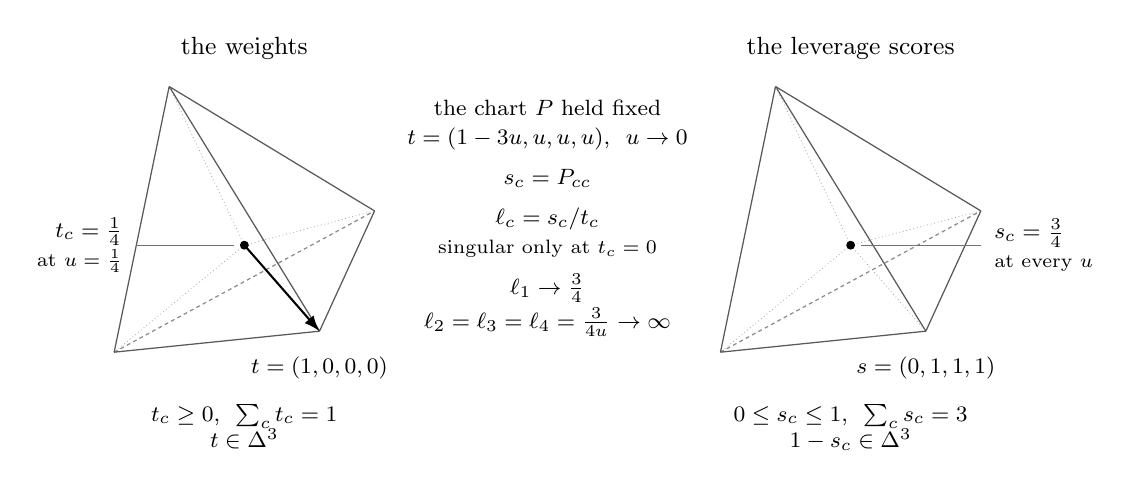
\begin{tikzpicture}[
  x=1cm, y=1cm,
  vec/.style={-{Latex[length=2mm,width=1.5mm]}, line width=0.75pt},
  frame/.style={densely dotted, line width=0.3pt, black!35},
  lead/.style={line width=0.3pt, black!55},
  edge/.style={line width=0.45pt, black!65},
  hidden/.style={line width=0.45pt, black!45, dashed, dash pattern=on 1.4pt off 1.2pt},
  every node/.style={font=\small}]

% ---- one simplex, vertices e_1..e_4, barycentre at the origin -----------
% projected vertices:  e_1 -> ( 1, 1, 1) -> ( 0.9546,-1.0920)
%                      e_2 -> ( 1,-1,-1) -> (-1.6534,-1.3588)
%                      e_3 -> (-1, 1,-1) -> ( 1.6534, 0.4354)
%                      e_4 -> (-1,-1, 1) -> (-0.9546, 2.0154)
% e_2--e_3 is the far diagonal of the silhouette quadrilateral, hence hidden;
% the four dotted medians locate the barycentre against the vertices.
\newcommand{\simplexframe}{%
  \draw[hidden] (-1.6534,-1.3588)--( 1.6534, 0.4354);
  \draw[edge]   ( 0.9546,-1.0920)--(-1.6534,-1.3588)
                ( 0.9546,-1.0920)--( 1.6534, 0.4354)
                ( 0.9546,-1.0920)--(-0.9546, 2.0154)
                (-1.6534,-1.3588)--(-0.9546, 2.0154)
                ( 1.6534, 0.4354)--(-0.9546, 2.0154);
  \draw[frame]  (0,0)--( 0.9546,-1.0920) (0,0)--(-1.6534,-1.3588)
                (0,0)--( 1.6534, 0.4354) (0,0)--(-0.9546, 2.0154);
  \fill (0,0) circle (1.6pt);}

% ======================= left: the weights ==============================
\simplexframe
\node[anchor=south] at (0,2.24) {the weights};
\draw[lead] (-0.13,0)--(-1.38,0);
\node[anchor=east, align=right, font=\footnotesize] at (-1.42,0)
  {$t_c=\tfrac14$\\[1pt] {\scriptsize at $u=\tfrac14$}};
% the escape path t = (1-3u, u, u, u) is the median from the barycentre to e_1
\draw[vec] (0,0)--( 0.9546,-1.0920);
\node[anchor=north, font=\footnotesize] at (0.9546,-1.30) {$t=(1,0,0,0)$};
\node[anchor=north, align=center, font=\footnotesize] at (0,-1.90)
  {$t_c\ge0$, \ $\sum_c t_c=1$\\ $t\in\Delta^{3}$};

% ======================= middle: what each coordinate does ==============
\node[align=center, font=\footnotesize] at (3.85,0.34)
  {the chart $P$ held fixed\\[1pt]
   $t=(1-3u,u,u,u)$, \ $u\to0$\\[5pt]
   $s_c=P_{cc}$\\[5pt]
   $\ell_c=s_c/t_c$\\[1pt]
   {\scriptsize singular only at $t_c=0$}\\[5pt]
   $\ell_1\to\tfrac34$\\[1pt]
   $\ell_2=\ell_3=\ell_4=\tfrac{3}{4u}\to\infty$};

% ======================= right: the leverage scores =====================
\begin{scope}[shift={(7.7,0)}]
  \simplexframe
  \node[anchor=south] at (0,2.24) {the leverage scores};
  \draw[lead] (0.13,0)--(1.66,0);
  \node[anchor=west, align=left, font=\footnotesize] at (1.70,0)
    {$s_c=\tfrac34$\\[1pt] {\scriptsize at every $u$}};
  \node[anchor=north, font=\footnotesize] at (0.9546,-1.30) {$s=(0,1,1,1)$};
  \node[anchor=north, align=center, font=\footnotesize] at (0,-1.90)
    {$0\le s_c\le1$, \ $\sum_c s_c=3$\\ $1-s_c\in\Delta^{3}$};
\end{scope}

\end{tikzpicture}

  \caption{The two simplices at $(4,3)$.  Left: the weights, in
  $\Delta^{3}$.  Right: the leverage scores, confined by
  Lemmas~\ref{lem:trace} and~\ref{lem:share} to
  $\{s\in[0,1]^{4}:\sum_c s_c=3\}$, which at corank one is again
  $\Delta^{3}$, in the coordinates $1-s_c$.  The tetrahedron design of
  Example~\ref{ex:tetra} is the barycentre of each.  With its chart held
  fixed (Lemma~\ref{lem:realize}) the weights run to a vertex while the
  leverage scores stand still, and the leverages $\ell_c=s_c/t_c$
  diverge; Example~\ref{ex:escape} is the same motion at $(2,1)$.  The
  leverage score is the coordinate that stays compact and the weight the
  one that reaches the boundary, so the compactification is taken in
  $(P,t)$ rather than in the design data.}
  \label{fig:twosimplices}
\end{figure}

\begin{definition}\label{def:chartpoint}
A \emph{chart point} of size $m$ and rank $k$ is a pair $(P,t)$ in which
$P$ is a real symmetric idempotent $m\times m$ matrix with $\tr P=k$ and
$t$ lies in the closed simplex
$\Delta^{m-1}=\{t\in\R^m:t_c\ge0,\ \sum_ct_c=1\}$.  Put $D:=\diag(t)$,
$W:=P-D$, and
\begin{equation}\label{eq:objective}
  G(P,t)\;:=\;\max_{\lvert C\rvert=k}\;\lmin\bigl(W[C]\bigr) .
\end{equation}
A $k$-subset $C$ \emph{dominates} at $(P,t)$ if $W[C]\psd0$.  Write
$\Gtz^{\mathrm{ch}}(m,k)$ for the assertion that every chart point of
size $m$ and rank $k$ admits a dominating $k$-subset.
\end{definition}

Since a maximum over a finite set is attained,
\begin{equation}\label{eq:threshold}
  G(P,t)\ge0
  \quad\Longleftrightarrow\quad
  \text{some $k$-subset dominates at $(P,t)$.}
\end{equation}
No condition ties $P$ to $t$.

The relation \eqref{eq:pivotlev} is the definition of $s_c$, not a
constraint, and on the compactification the vector lengths are recovered
only where $t_c>0$, by $\ell_c=P_{cc}/t_c$.  That formula is the
boundary's only singularity.

\begin{example}\label{ex:tetragap}
The tetrahedron of Example~\ref{ex:tetra} has $P=I_4-\tfrac14J_4$ and
$t_c=\tfrac14$ by Example~\ref{ex:tetrachart}, so
\[
  W\;=\;\tfrac34I_4-\tfrac14J_4,
  \qquad
  W[C]\;=\;\tfrac14\bigl(3I_3-J_3\bigr)
\]
at each of the four triples.  Since $J_3$ has eigenvalues $3,0,0$, the
spectrum of $W[C]$ is $\{0,\tfrac34,\tfrac34\}$, and $G(P,t)=0$: every
triple sits on the threshold and none crosses it, which is
\eqref{eq:threshold} read at a design whose triples are known to dominate
without slack.  The gap $\SC-I_3$ has spectrum $\{0,3,3\}$ by
\eqref{eq:tetraspec}, four times this one.
\end{example}

\begin{proposition}\label{prop:chartdesign}
The chart points of size $m$ and rank $k$ with $t_c>0$ for every $c$ are
exactly the chart points of designs of size $m$ and rank $k$ over $\R$,
and the design is determined by the chart point up to an orthogonal
transformation of $\R^k$.  Under this correspondence a $k$-subset dominates in the design
if and only if it dominates at the chart point.
\end{proposition}

\begin{proof}
A design produces $(VV\tp,t)$, which satisfies
Definition~\ref{def:chartpoint}.  Here $VV\tp$ is symmetric; it is
idempotent because $VV\tp VV\tp=V(V\tp V)V\tp$ and $V\tp V=I_k$, the
columns of $V$ being orthonormal; and $\tr(VV\tp)=\tr(V\tp V)=k$ by
cyclicity of the trace.  The weights lie in the open simplex.
Conversely let $(P,t)$ be a chart point with all weights positive.  A
symmetric idempotent is the orthogonal projection onto its range, and
its eigenvalues are $0$ and $1$, so its rank and its trace agree:
$\rk P=\tr P=k$.  Let the columns of the $m\times k$ matrix $V$ be an
orthonormal basis of that range, so that $P=VV\tp$ and $V\tp V=I_k$.
Write $v_c\tp$ for the $c$-th row of $V$ and put $g_c:=v_c/\sqrt{t_c}$.
Then
\[
  \sum_c t_c\,g_c^{\vphantom{\mathsf{T}}}g_c\tp
  \;=\;\sum_c v_c^{\vphantom{\mathsf{T}}}v_c\tp\;=\;V\tp V\;=\;I_k ,
\]
which is \eqref{eq:parseval}; the weights are positive and sum to one; so
this is a design, and its chart point is $(P,t)$.  Two orthonormal bases
of the range differ by an orthogonal $Q$, and the substitution
$V\mapsto VQ$ sends $g_c\mapsto Q\tp g_c$ and $\SC\mapsto Q\tp\SC Q$.
The comparison \eqref{eq:dominate} with $I_k$ survives because
$Q\tp I_kQ=I_k$.  The last assertion is Lemma~\ref{lem:chart}.
\end{proof}

\begin{lemma}\label{lem:compact}
The set of chart points of size $m$ and rank $k$ is compact, and
nonempty when $k\le m$.
\end{lemma}

\begin{proof}
It is the product of $\Delta^{m-1}$, which is compact, with the set
$\Pi_k$ of symmetric idempotents of trace $k$.  The three conditions
defining $\Pi_k$ are polynomial equations in the entries, so $\Pi_k$ is
closed; and for $P\in\Pi_k$,
\[
  \lVert P\rVert_{F}^{2}\;=\;\tr(P\tp P)\;=\;\tr(P^{2})\;=\;\tr P\;=\;k ,
\]
so $\Pi_k$ lies on a sphere of the Frobenius norm and is bounded, hence
compact.  It is the Grassmannian of $k$-planes in $\R^m$, nonempty for
$k\le m$.
\end{proof}

\begin{lemma}\label{lem:continuity}
$G$ is continuous.  Indeed, for chart points $(P,t)$ and $(Q,t')$ of the
same size and rank,
\[
  \bigl\lvert G(P,t)-G(Q,t')\bigr\rvert
  \;\le\;\lVert P-Q\rVert_{2}+\max_c\lvert t_c-t'_c\rvert ,
\]
where $\lVert\cdot\rVert_{2}$ is the operator norm.
\end{lemma}

\begin{proof}
For symmetric $A$ one has
$\lmin(A)=\min_{\lVert x\rVert=1}x\tp Ax$, an infimum of functions of $A$
each of which satisfies
$\lvert x\tp Ax-x\tp Bx\rvert\le\lVert A-B\rVert_{2}$ for
$\lVert x\rVert=1$.  Two infima over the same index set differ by at
most the supremum of the difference, so
$\lvert\lmin(A)-\lmin(B)\rvert\le\lVert A-B\rVert_{2}$.  Restriction to
the principal block on an index set $C$ is $A\mapsto E\tp AE$, where the
columns of $E$ are the coordinate vectors $e_c$ with $c\in C$, so it
does not increase the operator norm.  The two gap matrices differ by
$(P-Q)-\diag(t-t')$, of operator norm at most
$\lVert P-Q\rVert_{2}+\max_c\lvert t_c-t'_c\rvert$.  So each of the
finitely many functions $(P,t)\mapsto\lmin(W[C])$ obeys the stated bound,
and so does their maximum.
\end{proof}

Chart points with positive weights are dense, by a mixing of the weights
that recurs twice below.

\begin{lemma}\label{lem:relax}
Let $(P,t)$ be a chart point of size $m$ and rank $k$, let
$\bar t:=(1/m,\dots,1/m)$ and, for $0\le\theta\le1$, put
$t^{\theta}:=(1-\theta)t+\theta\bar t$.  Then $(P,t^{\theta})$ is a chart
point, its weights are strictly positive for $\theta>0$, and for every
$x\in\R^m$
\begin{equation}\label{eq:relax}
  x\tp W^{\theta}x\;=\;x\tp Wx-\theta\sum_c
    \Bigl(\frac1m-t_c\Bigr)x_c^{2},
  \qquad W^{\theta}:=P-\diag(t^{\theta}) .
\end{equation}
Consequently the chart points with strictly positive weights are dense,
and
\[
  \min G\;=\;\inf\{\,G(P,t):\text{$(P,t)$ the chart point of a design}\,\}.
\]
\end{lemma}

\begin{proof}
The simplex is convex, so $t^{\theta}\in\Delta^{m-1}$, and
$t^{\theta}_c\ge\theta/m>0$ for $\theta>0$; $P$ is untouched.  Identity
\eqref{eq:relax} is
$\diag(t^{\theta})=\diag(t)+\theta\diag(\bar t-t)$ evaluated against $x$.
Letting $\theta\to0$ gives $t^{\theta}\to t$, which is the density
statement.  For the equality of extrema, $\min G$ exists by
Lemmas~\ref{lem:compact} and~\ref{lem:continuity}, and is at most the
infimum, a minimum over the chart points being at most an infimum over
some of them.  For the reverse, apply the mixing to an arbitrary chart
point $(A,u)$: at $\theta>0$ the weights of $u^{\theta}$ are strictly
positive, so $(A,u^{\theta})$ is the chart point of a design by
Proposition~\ref{prop:chartdesign}, and $G(A,u^{\theta})$ is at least
the infimum.  Lemma~\ref{lem:continuity} along $u^{\theta}\to u$ carries
that bound to $G(A,u)$, and in particular to the minimum.
\end{proof}

The design space itself admits no such statement.  It is the locus
$t_c>0$, which is open in the compactification and, by
Example~\ref{ex:escape}, not closed in it; a minimizing sequence of
designs need not converge to a design.

\subsection{The two objectives}\label{sec:objectives}

The objective \eqref{eq:objective} is not the design objective $F$ of
\eqref{eq:value}.  With
$D[C]=\diag(t_c)_{c\in C}$ the congruence \eqref{eq:congruence} reads
$W[C]=D[C]^{1/2}\bigl(\Gram_C-I_k\bigr)D[C]^{1/2}$ --- the Gram matrix,
not the subset sum --- so that, substituting $x=D[C]^{-1/2}y$,
\[
  \frac{x\tp W[C]x}{x\tp D[C]x}
  \;=\;\frac{y\tp(\Gram_C-I_k)y}{\lVert y\rVert^{2}} .
\]
For $\lvert C\rvert=k$ the matrix $M_C$ is square, so $\Gram_C=M_CM_C\tp$
and $\SC=M_C\tp M_C$ have the same characteristic polynomial and hence the
same least eigenvalue; minimizing the last display over $y\ne0$ therefore
gives $\lmin(\SC)-1$, and
\[
  F(\dsn)-1\;=\;\max_{\lvert C\rvert=k}\;\min_{x\ne0}
    \frac{x\tp W[C]x}{x\tp D[C]x},
\]
against $G=\max_C\min_{\lVert x\rVert=1}x\tp W[C]x$.

\begin{remark}\label{rem:objectives}
The two agree in sign, by \eqref{eq:threshold} and
Lemma~\ref{lem:chart}.  Beyond the sign they are related by a congruence
which is not a scalar unless the selected weights are equal, so they
need not share their minimizers.  The generalized form degenerates where
$D[C]$ becomes singular, that is on the points the compactification adds.
The absolute form does not.
\end{remark}

At a selection whose weights are all equal the congruence is that common
weight, and $\lmin(W[C])=t_c\bigl(\lmin(\SC)-1\bigr)$ at any $c\in C$.
Where the selected weights differ the factor differs with $C$, and the
order of two selections can invert.


Figure~\ref{fig:objectives} draws the two graphs and the six pairs.

\begin{figure}[ht]
  \centering
  % The design objective F against the chart objective G on one segment of
% weights at (4,2), and the six pairs read off at one point of that segment.
%
% PROJECTION.  There is none: the two drawn panels are graphs of functions of
% one real variable and the third panel is a table.  The two axis boxes are
% pgfplots boxes of exactly 5.8cm by 2.2cm (scale only axis), the upper with its
% south west corner at picture coordinate (0,0) and the lower at (0,-3.10cm), so
% the two share one abscissa and a vertical line at a given weight meets both at
% the same picture abscissa.  The maps from data to picture are
%   upper   X = 5.8 * t_0 / (2/3),   Y = 2.2 * (F-1) / 2.2
%   lower   X = 5.8 * t_0 / (2/3),   Y = 2.2 * G / 0.37
% and every plotted coordinate below is written in axis cs, that is as the pair
% (t_0, value), with its exact rational source in a trailing comment.  Decimals
% in the body are six-place roundings of those rationals and of nothing else:
%   4/15 = 0.266667   7/15 = 0.466667   8/15 = 0.533333   17/30 = 0.566667
%   3/5  = 0.6        19/30 = 0.633333  2/3  = 0.666667   1/6   = 0.166667
%   1/5  = 0.2        7/30 = 0.233333   1/3  = 0.333333
% The worst of them is off by 3.4e-7, which at 5.8cm over a range of 2/3
% displaces a point by 3e-6 cm.  The three marked weights are named outside both
% frames, at picture abscissae 5.8 * (8/15)/(2/3) = 4.64,
% 5.8 * (17/30)/(2/3) = 4.93 and 5.8 * (19/30)/(2/3) = 5.51: the two minimizers
% anchored south on the ordinate 2.30, clear of the upper frame, and the census
% weight anchored north on -0.23, centred in the 0.90-wide band that separates
% the two frames and that carries nothing else, the upper abscissa being left
% unlabelled.  The third panel sits at the abscissa 6.60, its two blocks anchored
% north west on the ordinates 2.42 and -1.60 with a rule between them on -1.42.
%
% THE CHART POINT, exactly.  On the index set {0,1,2,3},
%   P = [[4/5,2/5,0,0],[2/5,1/5,0,0],[0,0,1/2,1/2],[0,0,1/2,1/2]],
%   t = ( t_0, 2/3 - t_0, 1/6, 1/6 ),   0 <= t_0 <= 2/3 .
% The two diagonal blocks are u u^T/5 with u = (2,1) and w w^T/2 with w = (1,1);
% since ||u||^2 = 5 and ||w||^2 = 2 each is a rank-one orthogonal projection, so
% P^T = P, P^2 = P and tr P = 1 + 1 = 2.  The weights are nonnegative and sum to
% t_0 + (2/3 - t_0) + 1/6 + 1/6 = 1.  So (P,t) is a chart point of size four and
% rank two at every t_0, and the chart point of a design at every interior t_0.
%
% THE DESIGN, exactly.  The range of P is spanned by (2,1,0,0)/sqrt5 and
% (0,0,1,1)/sqrt2, so the rows of V are
%   v_0 = (2/sqrt5,0)  v_1 = (1/sqrt5,0)  v_2 = (0,1/sqrt2)  v_3 = (0,1/sqrt2)
% and g_c = v_c/sqrt(t_c) puts g_0, g_1 on the first axis of R^2 and g_2, g_3 on
% the second, with leverages and leverage scores
%   ell_0 = 4/(5 t_0)          s_0 = P_00 = 4/5
%   ell_1 = 1/(5(2/3 - t_0))   s_1 = P_11 = 1/5
%   ell_2 = ell_3 = 3          s_2 = s_3 = 1/2 .
% Parseval holds over the rationals at every interior t_0: sum_c t_c g_c g_c^T is
% diag(s_0 + s_1, s_2 + s_3) = diag(1,1) = I_2, and sum_c s_c = 2 = k.
%
% THE TWO OBJECTIVES.  For a mixed pair P_ab = 0, so W[C] = diag(A_a,A_b) with
% A_c = s_c - t_c, and Gram_C = diag(ell_a, ell_b).  A pair drawn from one block
% has parallel vectors, so there its Gram matrix is singular; sharing a
% characteristic polynomial with S_C, and S_C being positive semidefinite, that
% puts lmin(S_C) = 0.  And det(Gram_C - I_2) = -(ell_a + ell_b - 1) < 0, because
% ell_0 >= 6/5 at every interior t_0 and ell_2 = ell_3 = 3, so det W[C] < 0 by
% cor:minor.  (ell_1 is NOT bounded below by 6/5.  It rises from 3/10 at t_0 = 0
% and passes 6/5 only at t_0 = 1/2, so the bound must be carried by ell_0 alone.)
% The mixed pair {0,2} carries lmin(S_C) = min(ell_0,3) >= 6/5 and
% lmin(W[C]) = min(A_0,1/3) >= 2/15, above both, so neither maximum is attained
% inside a block.  The two indices of a mixed pair range independently over the
% blocks, so a maximum over mixed pairs of a minimum is the minimum of the two
% block maxima:
%   F = min( max(ell_0, ell_1), 3 ),      G = min( max(A_0, A_1), 1/3 ) .
% Here A_0 = 4/5 - t_0 and A_1 = t_0 - 7/15, of constant sum 1/3, so max(A_0,A_1)
% is a V with vertex at t_0 = 19/30 and value 1/6; and ell_0 falls while ell_1
% rises, so max(ell_0,ell_1) has its least value 3/2 at t_0 = 8/15.  Hence
% min G = 1/6 at t_0 = 19/30 and min F = 3/2 at t_0 = 8/15, each at that one
% weight and nowhere else.  Breakpoints of the two graphs:
%   F - 1 = 2 on (0,4/15];  4/(5t_0) - 1 on [4/15,8/15];
%           1/(5(2/3-t_0)) - 1 on [8/15,3/5];  2 on [3/5,2/3)
%   G     = 1/3 on [0,7/15];  4/5 - t_0 on [7/15,19/30];  t_0 - 7/15 on [19/30,2/3]
% with F-1 = 1/2 at 8/15, = 1 at 17/30, = 2 at 19/30, and G = 4/15 at 8/15,
% = 7/30 at 17/30, = 1/6 at 19/30, = 1/3 at 0, = 1/5 at 2/3.  On the whole
% segment F >= 3/2 and G >= 1/6, so the family carries no counterexample, and
% none is claimed: (4,2) is corank two, where the conjecture is a theorem.
%
% F IS A DESIGN OBJECTIVE, so it has no value at a weight no design charts, and
% the two endpoints of the segment are such weights.  Both horizontal segments
% are drawn closed all the same: at either end max(ell_0,ell_1) diverges while
% the truncating constant ell_2 = 3 binds, so F extends continuously with value
% 3.  G is defined at both endpoints, being a function of the chart point alone.
%
% THE CENSUS ABSCISSA.  t_0 = 17/30 lies in the open interval
% (8/15, 19/30) between the two minimizers, which is where the leverage maximum
% of the first block has moved to the index 1 while its slack maximum still sits
% at the index 0; the two objectives therefore select different pairs there, and
% 17/30 keeps every entry rational or a single surd.  At it t = (17,3,5,5)/30 and
% ell = (24/17, 2, 3, 3), and, least eigenvalue first,
%          spec(Gram_C - I_2)   spec W[C]
%   {0,1}  -1, 41/17            1/6 - sqrt37/15, 1/6 + sqrt37/15
%   {0,2}  7/17, 2              7/30, 1/3
%   {0,3}  7/17, 2              7/30, 1/3
%   {1,2}  1, 2                 1/10, 1/3
%   {1,3}  1, 2                 1/10, 1/3
%   {2,3}  -1, 5                -1/6, 5/6
% The {0,1} row: the trace is A_0 + A_1 = 1/3 and the determinant is
% (7/30)(1/10) - (2/5)^2 = -41/300, so the eigenvalues are
% (1/3 +- sqrt(1/9 + 41/75))/2 with 1/9 + 41/75 = 148/225.  The {2,3} row is the
% one whose selected weights agree: D[C] = I_2/6 there, and spec W[C] is
% spec(Gram_C - I_2) divided by 6, entry for entry.
%
% DISCLOSED.  NOTHING IN THIS FIGURE IS MECHANIZED.  Neither F nor G is a Lean
% definition -- the compactness development carries the predicate
% Gtz.ChartDominates and no real-valued chart objective -- and no declaration
% evaluates either at this chart point or exhibits this design.  The results the
% panels invoke (lem:congruence, lem:chart, cor:minor, thm:boundary) carry their
% own tags; the arithmetic here carries none.  Nearest miss, recorded so that a
% later reader does not take the absence for an oversight: the anonymous function
% sup'_{C in gates} lambdaMinMat(subsetSumRaw config C) - 1 appears inside
% Gtz.continuous_dominationMargin, and that is F - 1 in all but name.  It is not
% a definition, its maximum runs over a supplied gate family rather than over all
% k-subsets, its argument is an unconstrained pair (vectors, weights) with no
% Parseval condition, and nothing evaluates it anywhere.
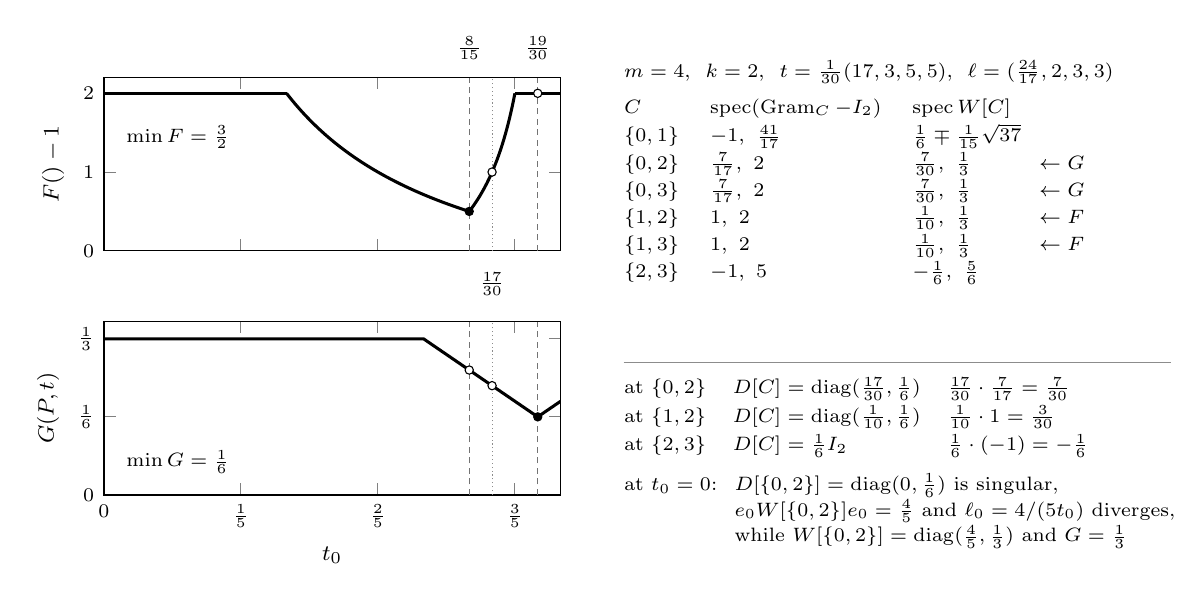
\begin{tikzpicture}[
  gcurve/.style={line width=1.1pt},
  guide/.style={line width=0.5pt, black!55, dashed,
                dash pattern=on 2.2pt off 1.6pt},
  census/.style={line width=0.4pt, black!45, densely dotted},
  hair/.style={line width=0.4pt, black!45}]

% ================= upper panel: the design objective F - 1 =================
\begin{axis}[
  name=Fax, at={(0,0)},
  width=5.8cm, height=2.2cm, scale only axis,
  xmin=0, xmax=0.666667, ymin=0, ymax=2.2,
  xtick={0,0.2,0.4,0.6}, xticklabel=\empty,
  ytick={0,1,2}, yticklabels={$0$,$1$,$2$},
  yticklabel style={font=\scriptsize},
  ylabel={$F(\dsn)-1$}, ylabel style={font=\footnotesize},
  tick style={line width=0.4pt}, axis line style={line width=0.5pt},
  clip=true]

\draw[guide]  (axis cs:0.533333,0) -- (axis cs:0.533333,2.2);   % t_0 = 8/15
\draw[guide]  (axis cs:0.633333,0) -- (axis cs:0.633333,2.2);   % t_0 = 19/30
\draw[census] (axis cs:0.566667,0) -- (axis cs:0.566667,2.2);   % t_0 = 17/30

\draw[gcurve] (axis cs:0,2)   -- (axis cs:0.266667,2);          % (0,2)--(4/15,2)
\draw[gcurve] (axis cs:0.6,2) -- (axis cs:0.666667,2);          % (3/5,2)--(2/3,2)
\addplot[gcurve, domain=0.266667:0.533333, samples=90]          % 4/(5t_0) - 1
  {4/(5*x) - 1};
\addplot[gcurve, domain=0.533333:0.6, samples=60]               % 1/(5(2/3-t_0)) - 1
  {1/(5*(0.666667 - x)) - 1};

\fill (axis cs:0.533333,0.5) circle (1.7pt);                    % (8/15, 1/2)
\draw[line width=0.4pt, fill=white]
      (axis cs:0.566667,1) circle (1.5pt)                       % (17/30, 1)
      (axis cs:0.633333,2) circle (1.5pt);                      % (19/30, 2)
\node[font=\scriptsize, anchor=west, inner sep=2pt]
  at (axis cs:0.024,1.44) {$\min F=\tfrac32$};
\end{axis}

% ================= lower panel: the chart objective G ======================
\begin{axis}[
  name=Gax, at={(0,-3.10cm)},
  width=5.8cm, height=2.2cm, scale only axis,
  xmin=0, xmax=0.666667, ymin=0, ymax=0.37,
  xtick={0,0.2,0.4,0.6}, xticklabels={$0$,$\tfrac15$,$\tfrac25$,$\tfrac35$},
  xticklabel style={font=\scriptsize},
  ytick={0,0.166667,0.333333}, yticklabels={$0$,$\tfrac16$,$\tfrac13$},
  yticklabel style={font=\scriptsize},
  xlabel={$t_0$}, ylabel={$G(P,t)$},
  xlabel style={font=\footnotesize}, ylabel style={font=\footnotesize},
  tick style={line width=0.4pt}, axis line style={line width=0.5pt},
  clip=true]

\draw[guide]  (axis cs:0.533333,0) -- (axis cs:0.533333,0.37);  % t_0 = 8/15
\draw[guide]  (axis cs:0.633333,0) -- (axis cs:0.633333,0.37);  % t_0 = 19/30
\draw[census] (axis cs:0.566667,0) -- (axis cs:0.566667,0.37);  % t_0 = 17/30

\draw[gcurve] (axis cs:0,0.333333)                              % (0, 1/3)
           -- (axis cs:0.466667,0.333333)                       % (7/15, 1/3)
           -- (axis cs:0.633333,0.166667)                       % (19/30, 1/6)
           -- (axis cs:0.666667,0.2);                           % (2/3, 1/5)

\fill (axis cs:0.633333,0.166667) circle (1.7pt);               % (19/30, 1/6)
\draw[line width=0.4pt, fill=white]
      (axis cs:0.533333,0.266667) circle (1.5pt)                % (8/15, 4/15)
      (axis cs:0.566667,0.233333) circle (1.5pt);               % (17/30, 7/30)
\node[font=\scriptsize, anchor=west, inner sep=2pt]
  at (axis cs:0.024,0.070) {$\min G=\tfrac16$};
\end{axis}

% ---- the three marked weights, named outside the frames ------------------
\node[font=\scriptsize, anchor=south] at (4.64,2.30) {$\tfrac8{15}$};
\node[font=\scriptsize, anchor=south] at (5.51,2.30) {$\tfrac{19}{30}$};
\node[font=\scriptsize, anchor=north, inner sep=1pt]
  at (4.93,-0.23) {$\tfrac{17}{30}$};

% ============ the six pairs at t_0 = 17/30, and the boundary ==============
\node[anchor=north west, align=left, font=\scriptsize, inner sep=0pt]
  at (6.60,2.42) {%
  $m=4$, \ $k=2$, \ $t=\tfrac1{30}(17,3,5,5)$, \
  $\ell=(\tfrac{24}{17},2,3,3)$\\[4pt]
  \begin{tabular}{@{}l@{\hspace{1.4em}}l@{\hspace{1.4em}}l@{\hspace{0.8em}}l@{}}
    $C$ & $\operatorname{spec}(\Gram_C-I_2)$ & $\operatorname{spec}W[C]$ &\\[1.5pt]
    $\{0,1\}$ & $-1,\ \tfrac{41}{17}$ & $\tfrac16\mp\tfrac1{15}\sqrt{37}$ &\\[1.5pt]
    $\{0,2\}$ & $\tfrac7{17},\ 2$ & $\tfrac7{30},\ \tfrac13$ & $\leftarrow G$\\[1.5pt]
    $\{0,3\}$ & $\tfrac7{17},\ 2$ & $\tfrac7{30},\ \tfrac13$ & $\leftarrow G$\\[1.5pt]
    $\{1,2\}$ & $1,\ 2$ & $\tfrac1{10},\ \tfrac13$ & $\leftarrow F$\\[1.5pt]
    $\{1,3\}$ & $1,\ 2$ & $\tfrac1{10},\ \tfrac13$ & $\leftarrow F$\\[1.5pt]
    $\{2,3\}$ & $-1,\ 5$ & $-\tfrac16,\ \tfrac56$ &\\
  \end{tabular}};

\draw[hair] (6.60,-1.42) -- (13.55,-1.42);

\node[anchor=north west, align=left, font=\scriptsize, inner sep=0pt]
  at (6.60,-1.60) {%
  \begin{tabular}{@{}l@{\hspace{1.2em}}l@{\hspace{1.2em}}l@{}}
    at $\{0,2\}$ & $D[C]=\diag(\tfrac{17}{30},\tfrac16)$
      & $\tfrac{17}{30}\cdot\tfrac7{17}=\tfrac7{30}$\\[2pt]
    at $\{1,2\}$ & $D[C]=\diag(\tfrac1{10},\tfrac16)$
      & $\tfrac1{10}\cdot1=\tfrac3{30}$\\[2pt]
    at $\{2,3\}$ & $D[C]=\tfrac16I_2$
      & $\tfrac16\cdot(-1)=-\tfrac16$\\
  \end{tabular}\\[5pt]
  at $t_0=0$: \ $D[\{0,2\}]=\diag(0,\tfrac16)$ is singular,\\
  \phantom{at $t_0=0$: \ }%
  $e_0\tp W[\{0,2\}]e_0=\tfrac45$ and $\ell_0=4/(5t_0)$ diverges,\\
  \phantom{at $t_0=0$: \ }%
  while $W[\{0,2\}]=\diag(\tfrac45,\tfrac13)$ and $G=\tfrac13$};

\end{tikzpicture}

  \caption{The two objectives at $(4,2)$, on the weight segment of
  Example~\ref{ex:objectives}.  Left: the design objective above the
  chart objective, on one abscissa; the marked weight $\tfrac8{15}$
  carries the least value of the first and $\tfrac{19}{30}$ that of the
  second, and at $\tfrac{19}{30}$ the first is $3$ while at $\tfrac8{15}$
  the second is $\tfrac4{15}$.  Right: the six pairs at the dotted weight
  $\tfrac{17}{30}$, with an arrow on the pair each objective selects.
  The congruence \eqref{eq:congruence} makes the six rows agree in sign,
  by Sylvester's law, and lets them disagree in order: it carries the
  relative slack $\tfrac7{17}$ of $\{0,2\}$ up to $\tfrac7{30}$ and the
  larger relative slack $1$ of $\{1,2\}$ down to $\tfrac3{30}$, being
  a scalar only at $\{2,3\}$, whose two weights agree.  At the endpoint
  $t_0=0$ the leverage $\ell_0$ diverges and the generalized quotient on
  $\{0,2\}$ is unbounded above, while the gap stays finite and $\{0,2\}$
  dominates.  Neither
  objective is a Lean definition, and none of the arithmetic here is
  mechanized.}
  \label{fig:objectives}
\end{figure}

\subsection{The boundary}\label{sec:boundary}

Let $(P,t)$ be a chart point with $t_z=0$ for some index $z$.  The
diagonal entry $P_{zz}$ decides which of two identities disposes of it,
and that entry is a squared length.

\begin{lemma}[Lean]\label{lem:pivot}
For every chart point and every index $z$,
\begin{equation}\label{eq:pivot}
  \lVert Pe_z\rVert^{2}\;=\;e_z\tp P\tp Pe_z\;=\;e_z\tp P^{2}e_z
  \;=\;e_z\tp Pe_z\;=\;P_{zz} .
\end{equation}
Hence $P_{zz}\ge0$; and $P_{zz}=0$ forces $Pe_z=0$, that is, the $z$-th
column and, by symmetry, the $z$-th row of $P$ vanish identically.
\end{lemma}

\begin{proof}
The chain \eqref{eq:pivot} uses symmetry and idempotency in that order.
A vanishing sum of squares $\sum_cP_{cz}^{2}=P_{zz}=0$ has all terms
zero.
\end{proof}

By \eqref{eq:pivotlev} the quantity $P_{zz}$ is the limit of the leverage
score $s_z$.

The dichotomy is therefore the distinction between the two ways an atom
can leave a design: its Parseval mass vanishes, or its mass survives
while its weight vanishes and its vector escapes to infinity.
Example~\ref{ex:escape} is of the second kind, with $P_{zz}=\tfrac12$.

\subsubsection*{Case A: the atom vanishes}

\begin{lemma}[Lean]\label{lem:delete}
Let $(P,t)$ be a chart point of size $m$ and rank $k$ and let $z$ satisfy
$t_z<1$ and $Pe_z=0$.  Delete the index $z$: let $\widehat P$ be the
principal submatrix of $P$ on the remaining indices and
$\widehat t_c:=t_c/(1-t_z)$.  Then $(\widehat P,\widehat t)$ is a chart
point of size $m-1$ and rank $k$, and for every $y\in\R^m$ with $y_z=0$,
writing $\widehat y$ for its restriction,
\begin{equation}\label{eq:reweight}
  y\tp Wy\;=\;\widehat y\tp\widehat W\widehat y
    +\frac{t_z}{1-t_z}\sum_{c\ne z}t_cy_c^{2}
  \;\ge\;\widehat y\tp\widehat W\widehat y .
\end{equation}
Consequently a subset dominating at $(\widehat P,\widehat t)$ dominates,
under the inclusion of index sets, at $(P,t)$.
\end{lemma}

\begin{proof}
Symmetry is inherited.  Since the $z$-th row and column of $P$ vanish,
the deleted index contributes nothing to any product, so
$\widehat P\widehat P$ is the corresponding submatrix of $P^{2}=P$, and
$\tr\widehat P=\tr P-P_{zz}=k$.  The weights $\widehat t_c$ are
nonnegative and sum to $(1-t_z)/(1-t_z)=1$.  For the identity, $y_z=0$
gives $y\tp Py=\widehat y\tp\widehat P\widehat y$, while
\[
  \widehat y\tp\diag(\widehat t)\widehat y-y\tp Dy
  \;=\;\sum_{c\ne z}\Bigl(\frac{t_c}{1-t_z}-t_c\Bigr)y_c^{2}
  \;=\;\frac{t_z}{1-t_z}\sum_{c\ne z}t_cy_c^{2},
\]
which is \eqref{eq:reweight} after subtraction.  The right-hand side is
nonnegative because $t_z\ge0$ and $t_z<1$.
\end{proof}

The reweighting is favourable at every admissible $t_z$, not only at
$t_z=0$; the hypothesis $t_z=0$ is needed only at the pivot of the next
case, where \S\ref{sec:sharp} locates the failure.

\subsubsection*{Case B: the direction escapes}

\begin{lemma}[Lean]\label{lem:deflate}
Let $(P,t)$ be a chart point of size $m$ and rank $k\ge1$ and let
$P_{zz}>0$.  Then
\begin{equation}\label{eq:deflate}
  P'\;:=\;P-\frac{(Pe_z)(Pe_z)\tp}{P_{zz}}
\end{equation}
is symmetric and idempotent with $\tr P'=k-1$ and $P'e_z=0$.  Hence
$(P',t)$ is a chart point of size $m$ and rank $k-1$ whose $z$-th row and
column vanish.
\end{lemma}

\begin{proof}
Write $r:=Pe_z$ and $R:=rr\tp$, so that $P'=P-R/P_{zz}$; symmetry is
clear.  Idempotency of $P$ gives $Pr=P^{2}e_z=Pe_z=r$, hence $PR=R$ and,
transposing, $RP=R$.  Lemma~\ref{lem:pivot} gives
$RR=r(r\tp r)r\tp=P_{zz}R$.  Therefore
\[
  \Bigl(P-\frac{R}{P_{zz}}\Bigr)^{2}
  \;=\;P^{2}-\frac{PR+RP}{P_{zz}}+\frac{RR}{P_{zz}^{2}}
  \;=\;P-\frac{2R}{P_{zz}}+\frac{R}{P_{zz}}
  \;=\;P-\frac{R}{P_{zz}} .
\]
The trace drops by $\tr R/P_{zz}=\lVert r\rVert^{2}/P_{zz}=1$, again by
\eqref{eq:pivot}.  Finally $r\tp e_z=P_{zz}$, so
$P'e_z=r-r\,P_{zz}/P_{zz}=0$.
\end{proof}

Deflation compresses the surviving vectors onto the orthogonal complement
of the escaping direction, carried out in the chart: on the surviving
indices $P'$ is the Schur complement of the pivot $P_{zz}$ in $P$.  The
computation chooses no basis of that complement and takes no square root.
It performs one division, by the pivot.  Since $P=P'+rr\tp/P_{zz}$ with
$r=Pe_z$, for every $x\in\R^m$
\begin{equation}\label{eq:transverse}
  x\tp Wx\;=\;x\tp(P'-D)x+\frac{\langle Pe_z,x\rangle^{2}}{P_{zz}} ,
\end{equation}
so the gap form upstairs exceeds the deflated one by the rank-one pivot
term.  Splitting the probe along the escaping coordinate isolates that
term.

\begin{lemma}\label{lem:schur}
Let $(P,t)$ be a chart point with $P_{zz}>0$ and let $P'$ be as in
\eqref{eq:deflate}.  Write $x=y+x_ze_z$ with $y_z=0$.  Then
\begin{equation}\label{eq:schur}
  x\tp Wx\;=\;y\tp(P'-D)\,y
    \;+\;\frac{\bigl(\langle Pe_z,y\rangle+x_zP_{zz}\bigr)^{2}}{P_{zz}}
    \;-\;t_z\,x_z^{2} .
\end{equation}
\end{lemma}

\begin{proof}
Expand $x\tp Px$ against the coordinate spike.  With
$a:=\langle Pe_z,y\rangle$ and $e_z\tp Pe_z=P_{zz}$,
\[
  x\tp Px\;=\;y\tp Py+2x_za+x_z^{2}P_{zz},
\]
and $P=P'+rr\tp/P_{zz}$ gives
$y\tp Py=y\tp P'y+a^{2}/P_{zz}$.  Since $y_z=0$,
$x\tp Dx=y\tp Dy+t_zx_z^{2}$.  Subtracting,
\[
  x\tp Wx\;=\;y\tp(P'-D)y
    +\frac{a^{2}}{P_{zz}}+2x_za+x_z^{2}P_{zz}-t_zx_z^{2} .
\]
The three middle terms complete a square: since $P_{zz}>0$,
\[
  \frac{a^{2}}{P_{zz}}+2x_za+x_z^{2}P_{zz}
  \;=\;\frac{a^{2}+2x_zaP_{zz}+x_z^{2}P_{zz}^{2}}{P_{zz}}
  \;=\;\frac{\bigl(a+x_zP_{zz}\bigr)^{2}}{P_{zz}} ,
\]
which is the middle term of \eqref{eq:schur}.
\end{proof}

Identity \eqref{eq:schur} is exact at every weight.  Its three terms are,
in order: the deflated gap, a square, and a deficit proportional to the
weight at the pivot.  At $t_z=0$ the deficit is absent and the lift
follows.

\begin{theorem}[Lean]\label{thm:schurstep}
Let $(P,t)$ be a chart point of size $m$ and rank $k\ge1$, let $z$
satisfy $P_{zz}>0$ and $t_z=0$, and let $C$ be a subset of the remaining
indices dominating at the chart point $(P',t)$ of rank $k-1$.  Then
$C\cup\{z\}$ dominates at $(P,t)$.
\end{theorem}

\begin{proof}
Let $x$ be supported on $C\cup\{z\}$ and split $x=y+x_ze_z$ with $y_z=0$;
then $y$ is supported on $C$, so $y\tp(P'-D)y\ge0$ by hypothesis.  In
\eqref{eq:schur} the last term vanishes because $t_z=0$, and the middle
term is nonnegative because $P_{zz}>0$.  Hence $x\tp Wx\ge0$.
\end{proof}

The pivot matches because the weight there is zero: the deflation
\eqref{eq:deflate} subtracts $P_{zz}$ from the diagonal at $z$, and
\eqref{eq:schur} restores the same amount.  The lift consumes the
rank-one excess of \eqref{eq:transverse} in full, so none of it is slack.

\begin{example}\label{ex:escapeb}
Return to Example~\ref{ex:escape}.  At its limit point, $z=2$,
$P_{zz}=\tfrac12$
and $t_z=0$.  Here $Pe_2=(\tfrac12,\tfrac12)\tp$ with
$\lVert Pe_2\rVert^{2}=\tfrac12=P_{22}$, as \eqref{eq:pivot} requires,
and \eqref{eq:deflate} gives $P'=P-2\cdot\tfrac14
\left(\begin{smallmatrix}1&1\\1&1\end{smallmatrix}\right)=0$, of trace
$0=k-1$.  Deleting $z$ leaves the chart point of size $1$ and rank $0$,
at which the empty selection dominates; Theorem~\ref{thm:schurstep}
returns $\{2\}$, and indeed $W_{22}=P_{22}-t_2=\tfrac12\ge0$.
\end{example}

\subsubsection*{The dichotomy}

\begin{theorem}[Lean]\label{thm:boundary}
Let $m\ge2$ and $k\ge1$, and assume $\Gtz^{\mathrm{ch}}(m-1,k)$ and
$\Gtz^{\mathrm{ch}}(m-1,k-1)$.  Then every chart point of size $m$ and
rank $k$ with $t_z=0$ for some $z$ admits a dominating $k$-subset.
\end{theorem}

\begin{proof}
By Lemma~\ref{lem:pivot} either $P_{zz}=0$ or $P_{zz}>0$.

If $P_{zz}=0$ then $Pe_z=0$, and $t_z=0<1$, so Lemma~\ref{lem:delete}
produces a chart point of size $m-1$ and rank $k$.  By
$\Gtz^{\mathrm{ch}}(m-1,k)$ some $k$-subset dominates there, and by
\eqref{eq:reweight} its image dominates at $(P,t)$.

If $P_{zz}>0$, deflate: by Lemma~\ref{lem:deflate}, $(P',t)$ is a chart
point of rank $k-1$ whose $z$-th column vanishes, so
Lemma~\ref{lem:delete} applies to it and produces a chart point of size
$m-1$ and rank $k-1$.  By $\Gtz^{\mathrm{ch}}(m-1,k-1)$ some
$(k-1)$-subset $C$ dominates there; by \eqref{eq:reweight} it dominates
at $(P',t)$; and by Theorem~\ref{thm:schurstep}, $C\cup\{z\}$, of
cardinality $k$, dominates at $(P,t)$.
\end{proof}

Both branches reduce the size by one, so an induction on the dichotomy is
well founded on the size alone.

At $k=1$ the second hypothesis is
$\Gtz^{\mathrm{ch}}(m-1,0)$, which holds because the empty selection
dominates.  Every step of the reduction is an identity, so it consumes no
slack and stays compatible with Corollary~\ref{cor:nomargin}.
Figure~\ref{fig:boundary} separates the two branches.

\begin{corollary}[Lean]\label{cor:interiorcex}
Under the hypotheses of Theorem~\ref{thm:boundary}, every chart point of
size $m$ and rank $k$ admitting \emph{no} dominating $k$-subset has
$t_c>0$ for every $c$.
\end{corollary}

\begin{proof}
Contrapositive of Theorem~\ref{thm:boundary}.
\end{proof}

\begin{figure}[ht]
  \centering
  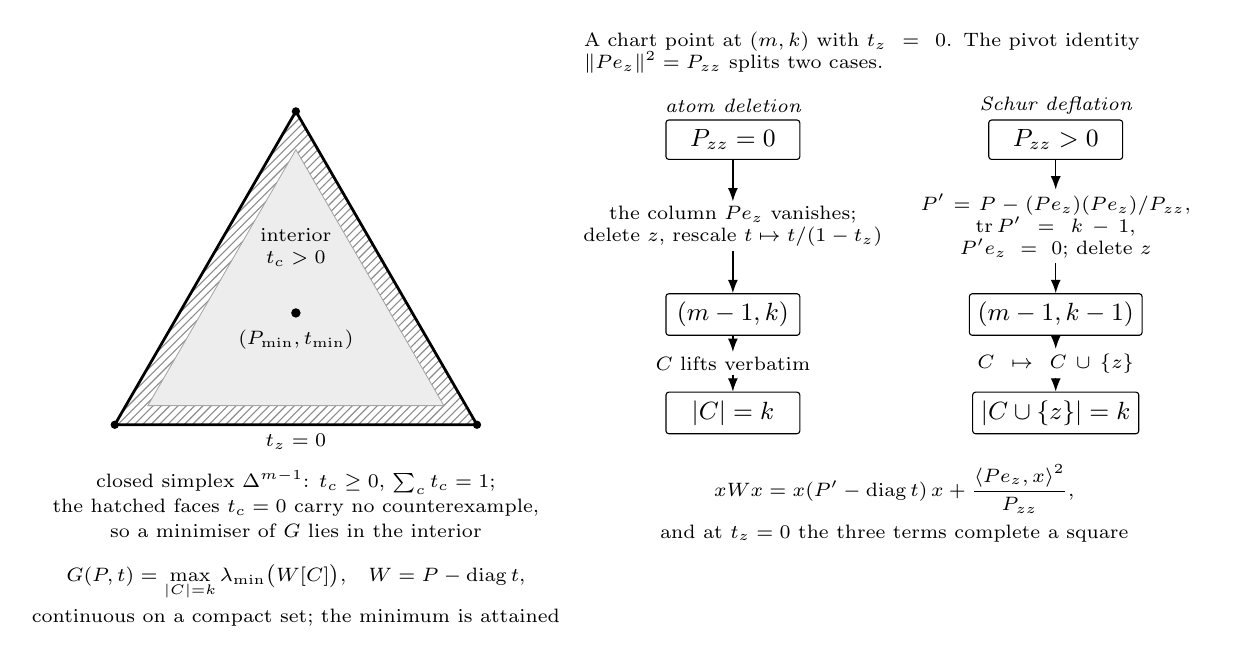
\begin{tikzpicture}[
  font=\small,
  bx/.style={draw, rounded corners=1pt, inner sep=3pt, minimum height=5mm,
             minimum width=17mm, align=center, font=\small},
  ar/.style={-{Latex[length=1.7mm]}, line width=0.5pt},
  ttl/.style={font=\scriptsize\itshape, align=center},
  txt/.style={font=\scriptsize, align=center, inner sep=1.5pt}]

% =====================================================================
% (a)  the compactification:  P fixed, t in the closed simplex
% =====================================================================
\begin{scope}
\coordinate (v1) at (0,0);
\coordinate (v2) at (4.6,0);
\coordinate (v3) at (2.3,3.98);
\coordinate (w1) at (0.42,0.243);
\coordinate (w2) at (4.18,0.243);
\coordinate (w3) at (2.3,3.494);

\fill[black!7] (w1) -- (w2) -- (w3) -- cycle;
\fill[pattern=north east lines, pattern color=black!45, even odd rule]
  (v1) -- (v2) -- (v3) -- cycle   (w1) -- (w2) -- (w3) -- cycle;
\draw[line width=1pt] (v1) -- (v2) -- (v3) -- cycle;
\draw[black!35, line width=0.3pt] (w1) -- (w2) -- (w3) -- cycle;
\foreach \p in {(v1),(v2),(v3)}{\fill \p circle (1.5pt);}

\node[txt] at (2.3,2.25) {interior\\ $t_c>0$};
\fill (2.3,1.42) circle (1.7pt);
\node[txt, anchor=north] at (2.3,1.26) {$(P_{\min},t_{\min})$};
\node[txt, anchor=north] at (2.3,-0.06) {$t_z=0$};

\node[txt, anchor=north] at (2.3,-0.52)
  {closed simplex $\Delta^{m-1}$: $t_c\ge0$, $\sum_c t_c=1$;\\[1pt]
   the hatched faces $t_c=0$ carry no counterexample,\\[1pt]
   so a minimiser of $G$ lies in the interior};
\node[txt, anchor=north] at (2.3,-1.72)
  {$G(P,t)=\displaystyle\max_{|C|=k}\lmin\bigl(W[C]\bigr)$,\quad $W=P-\diag t$,\\[2pt]
   continuous on a compact set; the minimum is attained};
\end{scope}

% =====================================================================
% (b)  the two boundary mechanisms at a vanishing weight
% =====================================================================
\begin{scope}[xshift=5.9cm]
\node[txt, anchor=north west, text width=79mm, align=left] at (0,5.05)
  {A chart point at $(m,k)$ with $t_z=0$. The pivot identity
   $\lVert Pe_z\rVert^{2}=P_{zz}$ splits two cases.};

% ---- case A : the atom vanishes -------------------------------------
\node[ttl] at (1.95,4.05) {atom deletion};
\node[bx] (a1) at (1.95,3.62) {$P_{zz}=0$};
\node[txt, text width=38mm, align=center] (a2) at (1.95,2.52)
  {the column $Pe_z$ vanishes;\\ delete $z$, rescale $t\mapsto t/(1-t_z)$};
\node[bx] (a3) at (1.95,1.40) {$(m-1,k)$};
\node[txt, text width=38mm, align=center] (a4) at (1.95,0.78) {$C$ lifts verbatim};
\node[bx] (a5) at (1.95,0.15) {$|C|=k$};
\draw[ar] (a1) -- (a2); \draw[ar] (a2) -- (a3);
\draw[ar] (a3) -- (a4); \draw[ar] (a4) -- (a5);

% ---- case B : deflation at the pivot --------------------------------
\node[ttl] at (6.05,4.05) {Schur deflation};
\node[bx] (b1) at (6.05,3.62) {$P_{zz}>0$};
\node[txt, text width=38mm, align=center] (b2) at (6.05,2.52)
  {$P'=P-(Pe_z)(Pe_z)\tp/P_{zz}$,\\ $\tr P'=k-1$, $P'e_z=0$; delete $z$};
\node[bx] (b3) at (6.05,1.40) {$(m-1,k-1)$};
\node[txt, text width=38mm, align=center] (b4) at (6.05,0.78) {$C\mapsto C\cup\{z\}$};
\node[bx] (b5) at (6.05,0.15) {$|C\cup\{z\}|=k$};
\draw[ar] (b1) -- (b2); \draw[ar] (b2) -- (b3);
\draw[ar] (b3) -- (b4); \draw[ar] (b4) -- (b5);

% ---- the identity that pays for the second case ---------------------
\node[txt, anchor=north] at (4.0,-0.45)
  {$x\tp Wx=x\tp(P'-\diag t)\,x
    +\dfrac{\langle Pe_z,x\rangle^{2}}{P_{zz}}$,\\[3pt]
   and at $t_z=0$ the three terms complete a square};
\end{scope}

\end{tikzpicture}

  \caption{The compactification and the boundary dichotomy.  Left: the
  objective $G$ of \eqref{eq:objective} is continuous on a compact space,
  so it attains its minimum; Theorem~\ref{thm:boundary} empties the
  faces $t_z=0$ of counterexamples, which places a negative minimum in
  the interior.  Right: the two mechanisms, separated by the pivot
  identity \eqref{eq:pivot}.  At $P_{zz}=0$ the atom is deleted and the
  weights rescaled; at $P_{zz}>0$ the point is deflated by
  \eqref{eq:deflate} and the selected subset regains $z$, the deficit in
  \eqref{eq:schur} being absent because $t_z=0$.}
  \label{fig:boundary}
\end{figure}

\subsection{The principle}\label{sec:variational}

Corollary~\ref{cor:interiorcex} speaks about a given chart point.  The
closed statement and the statement about designs are the same statement,
so the hypotheses of Theorem~\ref{thm:boundary} are ordinary smaller
instances of the problem.

\begin{proposition}[Lean]\label{prop:density}
Write $\Gtz^{\mathrm{ch}}_{\circ}(m,k)$ for the assertion that every
chart point of size $m$ and rank $k$ with strictly positive weights
admits a dominating $k$-subset.  Then
$\Gtz^{\mathrm{ch}}_{\circ}(m,k)$ implies $\Gtz^{\mathrm{ch}}(m,k)$, at
the same size and rank.
\end{proposition}

\begin{proof}
Let $(P,t)$ be a chart point at which no $k$-subset dominates.  For each
of the finitely many $k$-subsets $C$ choose $x^{C}$ supported on $C$ with
$(x^{C})\tp Wx^{C}<0$.  The form is quadratic, so rescaling $x^{C}$ by
$u>0$ multiplies its value by $u^{2}$, and $x^{C}$ may be normalized to
$(x^{C})\tp Wx^{C}=-1$.  The common value lets one mixing parameter
serve every selection.  Put
$\mu_C:=\sum_c(1/m-t_c)(x^{C}_c)^{2}$ and
$\theta:=\bigl(1+\sum_C\lvert\mu_C\rvert\bigr)^{-1}\in(0,1]$.  By
\eqref{eq:relax},
\[
  (x^{C})\tp W^{\theta}x^{C}\;=\;-1-\theta\mu_C\;<\;0
  \qquad\text{for every }C,
\]
since
$\theta\lvert\mu_C\rvert\le\theta\sum_{C'}\lvert\mu_{C'}\rvert<1$, each
term being at most the whole sum.  So no $k$-subset dominates at
$(P,t^{\theta})$, whose weights are strictly positive by
Lemma~\ref{lem:relax}, contradicting
$\Gtz^{\mathrm{ch}}_{\circ}(m,k)$.
\end{proof}

\begin{corollary}\label{cor:equivalent}
The three statements $\Gtz(m,k)$, $\Gtz^{\mathrm{ch}}_{\circ}(m,k)$ and
$\Gtz^{\mathrm{ch}}(m,k)$ are equivalent, for every $m$ and $k$.
\end{corollary}

\begin{proof}
By Proposition~\ref{prop:chartdesign} the designs of size $m$ and rank
$k$ correspond to the chart points with positive weights, and domination
corresponds to domination; so $\Gtz(m,k)$ and
$\Gtz^{\mathrm{ch}}_{\circ}(m,k)$ are the same assertion.
Proposition~\ref{prop:density} gives
$\Gtz^{\mathrm{ch}}_{\circ}(m,k)\Rightarrow\Gtz^{\mathrm{ch}}(m,k)$, and
the converse is trivial, a chart point with positive weights being a
chart point.
\end{proof}

\begin{theorem}\label{thm:variational}
Let $m>k\ge1$ and assume $\Gtz(m-1,k)$ and $\Gtz(m-1,k-1)$.  If
$\Gtz(m,k)$ fails, then $G$ attains its minimum over the compact space of
chart points of size $m$ and rank $k$ at a point $(P_{\min},t_{\min})$
with
\[
  G(P_{\min},t_{\min})<0
  \qquad\text{and}\qquad
  (t_{\min})_c>0\ \text{ for every }c .
\]
In particular $(P_{\min},t_{\min})$ is the chart point of a design
$\dsn_{\min}$ of size $m$ and rank $k$; no $k$-subset dominates in
$\dsn_{\min}$; and $\dsn_{\min}$ minimizes $G$ over all designs of size $m$ and
rank $k$.
\end{theorem}

\begin{proof}
By Corollary~\ref{cor:equivalent} the hypotheses are
$\Gtz^{\mathrm{ch}}(m-1,k)$ and $\Gtz^{\mathrm{ch}}(m-1,k-1)$, so
Theorem~\ref{thm:boundary} and Corollary~\ref{cor:interiorcex} are
available at size $m$ and rank $k$.

A counterexample to $\Gtz(m,k)$ is a design in which no $k$-subset
dominates; by Proposition~\ref{prop:chartdesign} its chart point admits
no dominating $k$-subset, so $G<0$ there by \eqref{eq:threshold}, and the
minimum of $G$ is negative.  By Lemmas~\ref{lem:compact}
and~\ref{lem:continuity} that minimum is attained, at
$(P_{\min},t_{\min})$ say.  Then $G(P_{\min},t_{\min})<0$, so no
$k$-subset dominates at $(P_{\min},t_{\min})$, so $(t_{\min})_c>0$ for
every $c$ by Corollary~\ref{cor:interiorcex}, and $(P_{\min},t_{\min})$
is the chart point of a design $\dsn_{\min}$ by
Proposition~\ref{prop:chartdesign}.
Finally $\min G$ equals the infimum of $G$ over designs, by
Lemma~\ref{lem:relax}, so $\dsn_{\min}$ attains that infimum.
\end{proof}

At $(6,3)$ the hypotheses are $\Gtz(5,3)$ and $\Gtz(5,2)$, both
instances of Corollary~\ref{cor:corank}.  At $(7,3)$ they are
$\Gtz(6,3)$ and $\Gtz(6,2)$; the second is Theorem~\ref{thm:ranktwo},
and the first is the cell $(6,3)$ itself.
The two open cells of Corollary~\ref{cor:twocells} are therefore treated
in order: $(6,3)$ first, and its resolution supplies the hypothesis
needed at $(7,3)$.

By Corollary~\ref{cor:equivalent} the statement about chart points with
positive weights is the original problem.  The mixing of
Lemma~\ref{lem:relax} does move a counterexample into the interior, but
it destroys whatever distinguished the original point, so it cannot be
applied to a minimizer.  Minimizing over the design space directly fails
as well: that space is not compact, and a minimizing sequence of designs
need not converge to a design (Example~\ref{ex:escape}).  The minimum
exists only on the compactification, and
Corollary~\ref{cor:interiorcex} puts it back inside.

\begin{wip}
Transport stationarity across the congruence $D[C]^{1/2}$ of
Remark~\ref{rem:objectives}, or restate the system of
\S\ref{sec:interior} for $G$; either removes the hypothesis of
Definition~\ref{def:extremalcex} from Theorem~\ref{thm:rankthree}.
\end{wip}

\subsection{Sharpness of the boundary step}\label{sec:sharp}

Theorem~\ref{thm:schurstep} requires $t_z=0$ exactly.  Call the
\emph{compression lift} the composite of Lemma~\ref{lem:deflate},
Lemma~\ref{lem:delete} and Theorem~\ref{thm:schurstep}: deflate at $z$,
delete $z$, renormalize, lift a dominating subset back.  It is meaningful
at any $t_z<1$.  A minimizing-sequence argument would need the
compression lift and not the boundary statement, since along such a
sequence the weight at the escaping label is positive and merely tends to
zero.  The lift fails at every positive weight, and no threshold in $t_z$
repairs it.

\begin{lemma}\label{lem:pairdet}
Let $(P,t)$ be a chart point, let $z$ satisfy $P_{zz}>0$ and $t_z<1$, and
let $c\ne z$.  Let $P'$ be the deflation \eqref{eq:deflate} and let
$\varepsilon:=P'_{cc}-t_c/(1-t_z)$ be the gap of the compressed point at $c$.
Then
\begin{equation}\label{eq:family}
  \det W[\{c,z\}]
  \;=\;\varepsilon\,P_{zz}\;-\;t_z\Bigl(P_{cc}-t_c-\frac{t_cP_{zz}}{1-t_z}\Bigr) .
\end{equation}
\end{lemma}

\begin{proof}
By \eqref{eq:deflate}, $P'_{cc}=P_{cc}-P_{cz}^{2}/P_{zz}$, so
\[
  P_{cz}^{2}\;=\;P_{zz}\bigl(P_{cc}-P'_{cc}\bigr)
  \;=\;P_{zz}\Bigl(P_{cc}-\frac{t_c}{1-t_z}-\varepsilon\Bigr).
\]
Since $W[\{c,z\}]=
\left(\begin{smallmatrix}P_{cc}-t_c&P_{cz}\\P_{cz}&P_{zz}-t_z\end{smallmatrix}\right)$,
\begin{align*}
  \det W[\{c,z\}]
  &=(P_{cc}-t_c)(P_{zz}-t_z)
     -P_{zz}\Bigl(P_{cc}-\frac{t_c}{1-t_z}-\varepsilon\Bigr)\\
  &=P_{cc}P_{zz}-t_zP_{cc}-t_cP_{zz}+t_zt_c
     -P_{zz}P_{cc}+\frac{t_cP_{zz}}{1-t_z}+\varepsilon P_{zz}\\
  &=\varepsilon\,P_{zz}-t_z\Bigl(P_{cc}-t_c-\frac{t_cP_{zz}}{1-t_z}\Bigr),
\end{align*}
using $t_cP_{zz}/(1-t_z)-t_cP_{zz}=t_z\,t_cP_{zz}/(1-t_z)$ in the last
step.
\end{proof}

Identity \eqref{eq:family} separates the two contributions.
The compressed slack $\varepsilon$ enters undamped, with coefficient $P_{zz}>0$;
the weight at the pivot enters linearly, with a coefficient tending to
$P_{cc}-t_c(1+P_{zz})$ as $t_z\to0$.  Hold the chart and the survivor
fixed.  If $\varepsilon>0$ then the determinant tends to
$\varepsilon\,P_{zz}>0$, and the pair ceases to obstruct for all small
$t_z$.  If $\varepsilon=0$ then the determinant is
$-t_z(P_{cc}-t_c-t_cP_{zz}/(1-t_z))$, negative for every $t_z>0$ at which
the bracket is positive.

The lift therefore fails wherever the compressed slack vanishes against
a positive bracket, however small $t_z$ is.

\begin{example}\label{ex:liftfailure}
On the index set $\{0,1,2,3\}$ let
\begin{equation}\label{eq:liftchart}
  P\;=\;\frac13\begin{pmatrix}
    2&1&0&1\\ 1&1&1&0\\ 0&1&2&-1\\ 1&0&-1&1\end{pmatrix},
\end{equation}
and let the weights run over the one-parameter family
\begin{equation}\label{eq:liftweights}
  t_1=\tau,\quad t_0=t_2=t_3=\frac{1-\tau}{3}
  \qquad(0\le\tau\le1),
\end{equation}
whose member at $\tau=\tfrac14$ is the uniform vector.  Let $z=1$ be the
pivot and $c=0$ the survivor.  Write $M:=3P$.  The
ten inner products of the rows $m_0,\dots,m_3$ of $M$ are
\[
  \begin{array}{c|cccc}
   \langle m_i,m_j\rangle & j=0&1&2&3\\ \hline
   i=0 & 6&3&0&3\\
   1 & 3&3&3&0\\
   2 & 0&3&6&-3\\
   3 & 3&0&-3&3
  \end{array}
\]
that is, $M^{2}=3M$; hence $P^{2}=P$, and $P$ is symmetric with
$\tr P=(2+1+2+1)/3=2$.  So $(P,t)$ is a chart point of size $4$ and rank
$2$ for every $\tau$.

At the pivot, $P_{11}=\tfrac13$ and
$Pe_1=(\tfrac13,\tfrac13,\tfrac13,0)\tp$, so
$\lVert Pe_1\rVert^{2}=\tfrac13=P_{11}$, in accordance with
\eqref{eq:pivot}.  Deflation \eqref{eq:deflate} subtracts $\tfrac13$ from
every entry indexed in $\{0,1,2\}$:
\[
  P'\;=\;\frac13\begin{pmatrix}
    1&0&-1&1\\ 0&0&0&0\\ -1&0&1&-1\\ 1&0&-1&1\end{pmatrix},
  \qquad \tr P'=1 .
\]
Deleting the index $1$ leaves the three survivors with weights
$\bigl((1-\tau)/3\bigr)/(1-\tau)=\tfrac13$ each, independently of $\tau$.
The compressed gap at the survivor $0$ is therefore
\[
  \varepsilon\;=\;P'_{00}-\tfrac13\;=\;\tfrac13-\tfrac13\;=\;0
  \qquad\text{at every }\tau ,
\]
so $\{0\}$ dominates the compressed point --- with slack exactly zero, at
every parameter value.  Upstairs, by \eqref{eq:family} with $\varepsilon=0$,
$P_{zz}=\tfrac13$, $P_{cc}=\tfrac23$, $t_c=(1-\tau)/3$ and $t_z=\tau$,
\[
  \det W[\{0,1\}]
  \;=\;-\tau\Bigl(\frac23-\frac{1-\tau}{3}
      -\frac{1-\tau}{3}\cdot\frac{1/3}{1-\tau}\Bigr)
  \;=\;-\tau\cdot\frac{6-3(1-\tau)-1}{9}
  \;=\;-\frac{\tau(2+3\tau)}{9},
\]
negative for every $\tau>0$.  Explicitly
$W[\{0,1\}]=\left(\begin{smallmatrix}(1+\tau)/3&1/3\\
1/3&(1-3\tau)/3\end{smallmatrix}\right)$, and the probe
$x=(-1,1+\tau,0,0)$ gives
\begin{align*}
  x\tp Wx
  &\;=\;\frac{1+\tau}{3}-\frac{2(1+\tau)}{3}
      +\frac{(1-3\tau)(1+\tau)^{2}}{3}\\
  &\;=\;\frac{1+\tau}{3}\bigl(-1+(1-3\tau)(1+\tau)\bigr)
  \;=\;-\frac{(1+\tau)\tau(2+3\tau)}{3}.
\end{align*}
At $\tau=\tfrac14$ the block, its determinant and the probe $(1,-4)$ are
\[
  W[\{0,1\}]=\begin{pmatrix}5/12&1/3\\ 1/3&1/12\end{pmatrix},
  \qquad \det=-\tfrac{11}{144},
  \qquad (1,-4)\,W[\{0,1\}]\,(1,-4)\tp=-\tfrac{11}{12}.
\]
The leverages $P_{cc}/t_c$ at $\tau=\tfrac14$ are
$\tfrac83,\tfrac43,\tfrac83,\tfrac43$, all exceeding $1$, so the point is not
disposed of by deletion of a light atom.
\end{example}

\begin{wip}
Exhibit a one-parameter deformation of \eqref{eq:liftchart} with compressed
slack $\varepsilon>0$, and display the resulting determinant
$(3\varepsilon-2\tau-3\tau^{2})/9$ of \eqref{eq:family} changing sign at
$\tau\asymp \varepsilon$.
\end{wip}

\begin{theorem}[Lean]\label{thm:sharp}
There is no $\tau_0>0$ such that the compression lift holds at every
chart point with $t_z<\tau_0$.  Explicitly: for every $\tau_0>0$ there
are a chart point of size $4$ and rank $2$, a pivot $z$ with $P_{zz}>0$
and $0<t_z<\tau_0$, and a subset dominating the compressed point of size
$3$ and rank $1$, whose image together with $z$ does not dominate.
\end{theorem}

\begin{proof}
Take the family of Example~\ref{ex:liftfailure} at
$\tau=\min\{\tau_0,1\}/2$.  Then $0<\tau<\tau_0$ and $\tau<1$; the
compressed point is dominated by $\{0\}$, since its gap there is $0$; and
$\{0,1\}$ does not dominate upstairs, the probe $(-1,1+\tau,0,0)$ giving
$-(1+\tau)\tau(2+3\tau)/3<0$.
\end{proof}

The obstruction sits on the equality locus of \S\ref{sec:ties}.
Shrinking $t_z$ does shrink the deficit, but along this family it shrinks
nothing else: the compressed slack is frozen at zero, so the deficit is
never overtaken.  By \eqref{eq:family} a positive compressed slack would
overtake it, and no positive lower bound on $\varepsilon$ is to be had.
The compressed point is a chart point one size and one rank lower, hence
by Proposition~\ref{prop:chartdesign} the chart point of a design
wherever its weights are positive; and by
Theorem~\ref{thm:tieseverywhere} designs whose dominating subsets all
have $\lmin(\SC)=1$, that is with chart slack zero, exist at every cell
with $m\ge k+1$ and at every weight vector.

The compression sends the whole family to one point, the surviving
weights being $\tfrac13$ at every $\tau$.  That point charts the design
$g=(1,-1,1)$ at $(3,1)$, of leverage $1$ at each index, so each of its
singletons dominates with $\lmin(\SC)=1$.
Figure~\ref{fig:boundarytrace} runs the four steps and the fork on the
family.

\begin{figure}[ht]
  \centering
  % The boundary dichotomy executed on the chart point of ex:liftfailure at (4,2),
% with the intermediate matrix printed at every step, and the fork at the lift.
%
% PROJECTION.  There is none: the figure is a flow of text and matrices, and no
% space of dimension above zero is drawn.  The layout is a grid in picture
% centimetres, and every ordinate below is a node CENTRE, set so that
% consecutive boxes clear one another by about 9pt, which is twice the 1.7mm
% arrowhead that joins them.  The datum spans the top from the ordinate 9.15
% down.  The four steps of the compression are stacked in one column, centred at
% the abscissa 3.45 on the ordinates 6.52, 4.57, 2.22 and -0.01 under a title on
% 7.80, and joined downwards by arrows; they are the steps that do not see the
% parameter.  The stem at the abscissa 7.35 carries the compressed verdict into
% both branches, which are centred at the abscissa 11.35 on the ordinates 4.95
% and 1.93, with the identity they share above them on 7.80, a rule on 0.12, and
% the standing pair anchored north on -0.06.  Every number in the body is an
% entry of one of the matrices derived below, and no drawn coordinate carries
% data.
%
% THE CHART POINT, exactly, as in eq:liftchart and eq:liftweights.
%   P = (1/3) [[2,1,0,1],[1,1,1,0],[0,1,2,-1],[1,0,-1,1]],
%   t = ( (1-tau)/3, tau, (1-tau)/3, (1-tau)/3 ),   0 <= tau <= 1 .
% With M := 3P the ten inner products of the rows of M are
%   <m_0,m_0> = 6  <m_0,m_1> = 3  <m_0,m_2> = 0  <m_0,m_3> =  3
%   <m_1,m_1> = 3  <m_1,m_2> = 3  <m_1,m_3> = 0  <m_2,m_2> =  6
%   <m_2,m_3> = -3 <m_3,m_3> = 3
% that is M^2 = 3M, whence P^2 = P; P is symmetric and tr P = (2+1+2+1)/3 = 2.
% The weights are nonnegative and sum to 3*(1-tau)/3 + tau = 1.  So (P,t) is a
% chart point of size four and rank two at every tau in [0,1].
%
% THE RANGE.  ex:liftfailure declares 0 <= tau <= 1 and eq:liftweights the open
% interval, which is where the lift fails and where the chart point is the chart
% point of a design.  The figure takes the closed range: the left branch of the
% fork is the member at tau = 0, the one thm:schurstep applies to, and that
% member is a chart point and not a design.  Lean's Gtz.liftFailurePointAt
% carries the same closed range, 0 <= pivotWeight <= 1, and its frozen-slack
% theorem carries in addition the tau < 1 that STEP 3 needs.
%
% STEP 1, the pivot, at z = 1.  Column 1 of P is (1,1,1,0)/3, of squared length
% 3*(1/9) = 1/3, which is P_11: this is eq:pivot, and P_11 > 0 puts the point in
% the second branch of thm:boundary.
%
% STEP 2, deflation.  (P e_1)(P e_1)^T / P_11 = 3 * (1/9) J on the index block
% {0,1,2}, that is 1/3 at each of the nine entries indexed there and 0 elsewhere,
% so eq:deflate subtracts 1/3 from every entry indexed in {0,1,2}:
%   P' = (1/3) [[1,0,-1,1],[0,0,0,0],[-1,0,1,-1],[1,0,-1,1]] .
% With u = (1,0,-1,1) one has u u^T equal to that integer matrix and ||u||^2 = 3,
% so P' = u u^T/||u||^2 is the orthogonal projection on the line R u: symmetric,
% idempotent, of trace 1 = k - 1, with P' e_1 = 0.
%
% STEP 3, deletion.  Striking the row and column 1 leaves, on the survivors
% {0,2,3} in that order,
%   hat P = (1/3) [[1,-1,1],[-1,1,-1],[1,-1,1]] ,
% and lem:delete, whose hypothesis is t_z < 1, renormalizes each surviving weight
% to ((1-tau)/3)/(1-tau) = 1/3, the same number at every tau < 1: the compression
% sends the whole one-parameter family to one point.  This is the one step of the
% four that does not run at tau = 1.  That point has positive weights,
% so by prop:chartdesign it is the chart point of a design at (3,1); the rows of
% V are the entries of u/sqrt3 = (1,-1,1)/sqrt3, and g_c = v_c/sqrt(t_c) gives
%   g = (1,-1,1),   ell_c = 1,   sum_c t_c g_c^2 = 3*(1/3)*1 = 1 .
% Every singleton has S_C = 1, so every singleton dominates with equality: the
% compressed point lies on the equality locus of section sec:ties.
%
% STEP 4, the compressed gap.  hat W = hat P - diag(1/3,1/3,1/3) =
% (1/3)[[0,-1,1],[-1,0,-1],[1,-1,0]], whose diagonal is zero.  So the compressed
% slack of lem:pairdet is eps = hat W_00 = 0, at every tau.
%
% THE IDENTITY.  For x supported on {0,1}, write x = y + x_1 e_1 with y = x_0 e_0.
% Then <P e_1, y> = x_0/3, P'_00 - t_0 = 1/3 - (1-tau)/3 = tau/3, and eq:schur is
%   x^T W x = (tau/3) x_0^2 + (1/3)(x_0 + x_1)^2 - tau x_1^2 ,
% which expands to ((1+tau)/3)x_0^2 + (2/3)x_0 x_1 + (1/3 - tau)x_1^2, the form of
% W[{0,1}].  The three terms are the deflated gap, the square and the deficit.
%
% THE FORK.  At tau = 0 the deficit is absent and the first term vanishes with
% it, leaving (1/3)(x_0+x_1)^2 >= 0; there W[{0,1}] = (1/3)[[1,1],[1,1]], of trace
% 2/3 and determinant 0, hence of spectrum {0, 2/3}.  At tau > 0,
%   W[{0,1}] = [[(1+tau)/3, 1/3],[1/3, 1/3 - tau]],
%   det = ((1+tau)(1-3tau) - 1)/9 = -tau(2+3tau)/9 ,
% which is eq:family at eps = 0, P_zz = 1/3, P_cc = 2/3, t_c = (1-tau)/3; and the
% probe (-1, 1+tau, 0, 0) gives ((1+tau)/3)(1 - 2 + (1+tau)(1-3tau)) =
% -tau(1+tau)(2+3tau)/3.  At tau = 1/4 the block is [[5/12,1/3],[1/3,1/12]] of
% determinant 5/144 - 16/144 = -11/144, and (1,-4,0,0) gives
% 5/12 - 8/3 + 16/12 = -11/12.
%
% THE STANDING PAIR.  P_02 = 0, P_00 = P_22 = 2/3 and t_0 = t_2 = (1-tau)/3, so
% W[{0,2}] = ((1+tau)/3) I_2, positive semidefinite at every tau in [0,1].  The
% pair {0,2} therefore dominates throughout the family.
%
% DISCLOSED.  The Lean development carries the chart (symmetric, idempotent, of
% trace two), the one-parameter family, the frozen compressed slack and the
% failure of the lift at every positive weight, together with the three general
% steps; it does not state the displayed P', hat P and hat W, which are computed
% inside its proofs, and it does not state the standing pair {0,2}.  The passage
% from the compressed chart point to the design g = (1,-1,1) uses the half of
% prop:chartdesign that section sec:formalization records as not mechanized.
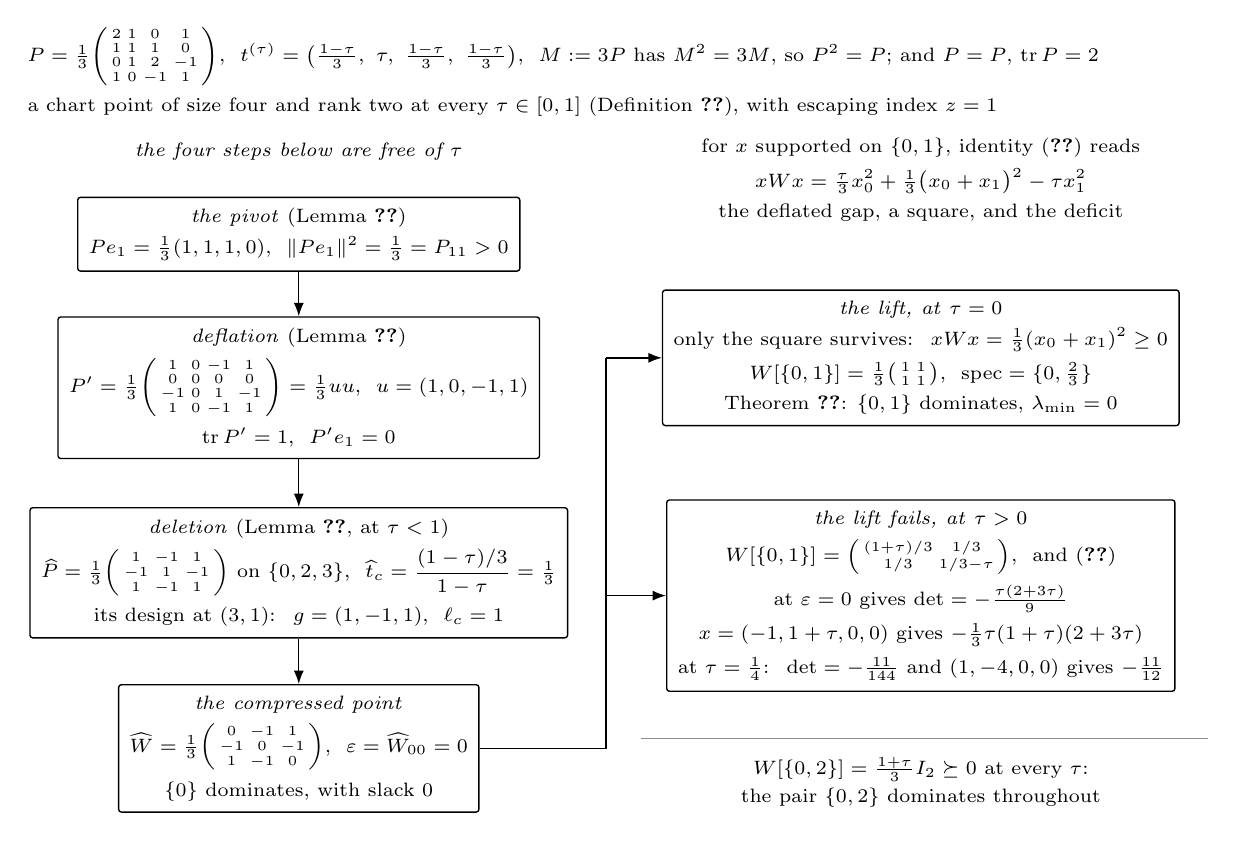
\begin{tikzpicture}[
  bx/.style={draw, rounded corners=1pt, line width=0.5pt, inner sep=4pt,
             align=center, font=\scriptsize},
  ar/.style={-{Latex[length=1.7mm]}, line width=0.5pt},
  ttl/.style={font=\scriptsize\itshape, align=center},
  txt/.style={font=\scriptsize, align=center, inner sep=1.5pt},
  hair/.style={line width=0.4pt, black!45}]

% ====================== the datum, spanning the top =======================
\node[anchor=north west, align=left, font=\scriptsize, inner sep=0pt]
  at (0,9.15) {%
  $P=\tfrac13\begin{psmallmatrix}2&1&0&1\\1&1&1&0\\0&1&2&-1\\
                                 1&0&-1&1\end{psmallmatrix}$, \
  $t^{(\tau)}=\bigl(\tfrac{1-\tau}{3},\ \tau,\ \tfrac{1-\tau}{3},
                    \ \tfrac{1-\tau}{3}\bigr)$, \
  $M:=3P$ has $M^{2}=3M$, so $P^{2}=P$; and $P\tp=P$, $\tr P=2$\\[3pt]
  a chart point of size four and rank two at every $\tau\in[0,1]$
  (Definition~\ref{def:chartpoint}), with escaping index $z=1$};

% ================ the compression, four steps, one column =================
\node[ttl, anchor=north] at (3.45,7.80) {the four steps below are free of
  $\tau$};

\node[bx] (s1) at (3.45,6.52) {%
  \textit{the pivot} (Lemma~\ref{lem:pivot})\\[3pt]
  $Pe_1=\tfrac13(1,1,1,0)\tp$, \
  $\lVert Pe_1\rVert^{2}=\tfrac13=P_{11}>0$};

\node[bx] (s2) at (3.45,4.57) {%
  \textit{deflation} (Lemma~\ref{lem:deflate})\\[3pt]
  $P'=\tfrac13\begin{psmallmatrix}1&0&-1&1\\0&0&0&0\\-1&0&1&-1\\
                                  1&0&-1&1\end{psmallmatrix}
      =\tfrac13uu\tp$, \ $u=(1,0,-1,1)$\\[3pt]
  $\tr P'=1$, \ $P'e_1=0$};

\node[bx] (s3) at (3.45,2.22) {%
  \textit{deletion} (Lemma~\ref{lem:delete}, at $\tau<1$)\\[3pt]
  $\widehat P=\tfrac13\begin{psmallmatrix}1&-1&1\\-1&1&-1\\
                                          1&-1&1\end{psmallmatrix}$
  on $\{0,2,3\}$, \
  $\widehat t_c=\dfrac{(1-\tau)/3}{1-\tau}=\tfrac13$\\[3pt]
  its design at $(3,1)$: \ $g=(1,-1,1)$, \ $\ell_c=1$};

\node[bx] (s4) at (3.45,-0.01) {%
  \textit{the compressed point}\\[3pt]
  $\widehat W=\tfrac13\begin{psmallmatrix}0&-1&1\\-1&0&-1\\
                                          1&-1&0\end{psmallmatrix}$, \
  $\varepsilon=\widehat W_{00}=0$\\[3pt]
  $\{0\}$ dominates, with slack $0$};

\draw[ar] (s1) -- (s2);
\draw[ar] (s2) -- (s3);
\draw[ar] (s3) -- (s4);

% ================= the identity that both branches read ===================
\node[txt, anchor=north] at (11.35,7.80) {%
  for $x$ supported on $\{0,1\}$, identity \eqref{eq:schur} reads\\[3pt]
  $x\tp Wx=\tfrac{\tau}{3}x_0^{2}
     +\tfrac13\bigl(x_0+x_1\bigr)^{2}-\tau x_1^{2}$\\[3pt]
  the deflated gap, a square, and the deficit};

% ================================ the fork ================================
\node[bx] (f0) at (11.35,4.95) {%
  \textit{the lift, at} $\tau=0$\\[3pt]
  only the square survives: \
  $x\tp Wx=\tfrac13(x_0+x_1)^{2}\ge0$\\[3pt]
  $W[\{0,1\}]=\tfrac13\begin{psmallmatrix}1&1\\1&1\end{psmallmatrix}$, \
  $\operatorname{spec}=\{0,\tfrac23\}$\\[3pt]
  Theorem~\ref{thm:schurstep}: $\{0,1\}$ dominates, $\lmin=0$};

\node[bx] (f1) at (11.35,1.93) {%
  \textit{the lift fails, at} $\tau>0$\\[3pt]
  $W[\{0,1\}]=\begin{psmallmatrix}(1+\tau)/3&1/3\\
                                  1/3&1/3-\tau\end{psmallmatrix}$, \
  and \eqref{eq:family}\\[3pt]
  at $\varepsilon=0$ gives $\det=-\tfrac{\tau(2+3\tau)}{9}$\\[3pt]
  $x=(-1,1+\tau,0,0)$ gives $-\tfrac13\tau(1+\tau)(2+3\tau)$\\[3pt]
  at $\tau=\tfrac14$: \ $\det=-\tfrac{11}{144}$ and
  $(1,-4,0,0)$ gives $-\tfrac{11}{12}$};

\draw[line width=0.5pt] (s4.east) -| (7.35,4.95);
\draw[ar] (7.35,4.95) -- (f0.west);
\draw[ar] (7.35,1.93) -- (f1.west);

% ========================== what stands throughout ========================
\draw[hair] (7.80,0.12) -- (15.00,0.12);
\node[txt, anchor=north] at (11.35,-0.06) {%
  $W[\{0,2\}]=\tfrac{1+\tau}{3}I_2\psd0$ at every $\tau$:\\[2pt]
  the pair $\{0,2\}$ dominates throughout};

\end{tikzpicture}

  \caption{The dichotomy of Theorem~\ref{thm:boundary} executed on the
  chart point of Example~\ref{ex:liftfailure}, at $(4,2)$ with pivot $z=1$.
  Left: the four steps of the compression lift, each with the matrix it
  produces; none of them sees $\tau$, and the deletion returns the same
  compressed point at every $\tau$, the chart point of the design
  $g=(1,-1,1)$ at $(3,1)$ on which every singleton dominates with
  $\lmin(\SC)=1$.  Right: identity \eqref{eq:schur} on the pair
  $\{0,1\}$, and the two branches it splits into.  At $\tau=0$ the
  deflated gap and the deficit vanish together and
  Theorem~\ref{thm:schurstep} lifts $\{0\}$ to $\{0,1\}$ with least
  eigenvalue $0$, so the lift leaves no slack.  At $\tau>0$ the deficit
  survives, and \eqref{eq:family} at $\varepsilon=0$ turns it into a
  negative determinant.  The pair $\{0,2\}$ dominates throughout the
  family, so what fails at positive weight is the lift rather than the
  chart point.}
  \label{fig:boundarytrace}
\end{figure}

This is Corollary~\ref{cor:nomargin} again, in local form.  It is why the
boundary is discharged at $t_z=0$ by the identity \eqref{eq:schur}
instead of at small $t_z$ by an estimate, and why
Theorem~\ref{thm:variational} speaks of the limit point rather than of a
minimizing sequence.  Figure~\ref{fig:sharp} shows the two contributions.

\begin{figure}[ht]
  \centering
  % Identity (eq:family) evaluated on the chart of section app:liftfail:
%   P_zz = 1/3, P_cc = 2/3, t_c = (1-t)/3, t_z = t,
%   det W[{c,z}] = d/3 - t(2+3t)/9 = (3d - 2t - 3t^2)/9 .
% Level v is the parabola  d = 3v + 2t/3 + t^2 ; the zero level is
%   d = 2t/3 + t^2 , tangent at the origin to the line d = 2t/3.
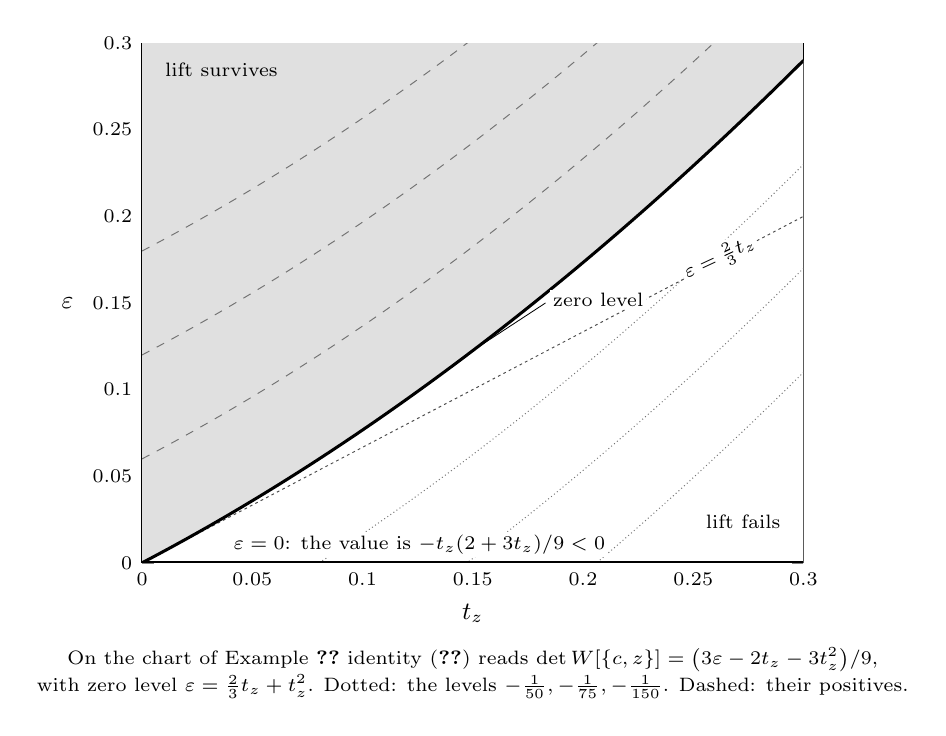
\begin{tikzpicture}
\begin{axis}[
  name=sharpaxis,
  width=8.4cm, height=6.6cm,
  scale only axis,
  xmin=0, xmax=0.3, ymin=0, ymax=0.3,
  xtick={0,0.05,0.1,0.15,0.2,0.25,0.3},
  ytick={0,0.05,0.1,0.15,0.2,0.25,0.3},
  xticklabel style={font=\scriptsize, /pgf/number format/fixed,
                    /pgf/number format/precision=2},
  yticklabel style={font=\scriptsize, /pgf/number format/fixed,
                    /pgf/number format/precision=2},
  xlabel={$t_z$}, ylabel={$\varepsilon$},
  xlabel style={font=\small}, ylabel style={font=\small, rotate=-90},
  samples=200, domain=0:0.3,
  clip=true]

% ---- the region where the lift survives -----------------------------
\fill[black!12] (axis cs:0,0) rectangle (axis cs:0.3,0.3);
\addplot[draw=none, fill=white] {2*x/3 + x^2} \closedcycle;

% ---- level curves  (3d - 2t - 3t^2)/9 = v ---------------------------
\addplot[black!55, line width=0.35pt, densely dotted] {2*x/3 + x^2 - 0.18};
\addplot[black!55, line width=0.35pt, densely dotted] {2*x/3 + x^2 - 0.12};
\addplot[black!55, line width=0.35pt, densely dotted] {2*x/3 + x^2 - 0.06};
\addplot[black!55, line width=0.35pt, dashed] {2*x/3 + x^2 + 0.06};
\addplot[black!55, line width=0.35pt, dashed] {2*x/3 + x^2 + 0.12};
\addplot[black!55, line width=0.35pt, dashed] {2*x/3 + x^2 + 0.18};

% ---- the tangent line d = 2t/3 at the origin ------------------------
\addplot[black!70, line width=0.35pt, dash pattern=on 1pt off 1.2pt]
  {2*x/3};

% ---- the zero level --------------------------------------------------
\addplot[black, line width=1.1pt] {2*x/3 + x^2};

% ---- the extremal axis d = 0 ----------------------------------------
\draw[line width=1.4pt] (axis cs:0,0) -- (axis cs:0.3,0);

% ---- labels inside the frame ----------------------------------------
\node[font=\scriptsize, anchor=north west] at (axis cs:0.006,0.294)
  {lift survives};
\node[font=\scriptsize, anchor=south east] at (axis cs:0.294,0.014)
  {lift fails};
\draw[line width=0.3pt] (axis cs:0.150,0.1225) -- (axis cs:0.183,0.150);
\node[font=\scriptsize, anchor=west, fill=white, inner sep=1pt]
  at (axis cs:0.185,0.152) {zero level};
\node[font=\scriptsize, rotate=25, fill=white, inner sep=1pt]
  at (axis cs:0.262,0.176) {$\varepsilon=\tfrac23 t_z$};
\node[font=\scriptsize, anchor=south west, fill=white, inner sep=1pt]
  at (axis cs:0.040,0.003) {$\varepsilon=0$: the value is $-t_z(2+3t_z)/9<0$};
\end{axis}

% ---- the reading of the picture, below the frame ---------------------
\node[font=\scriptsize, anchor=north, align=center]
  at ($(sharpaxis.south)+(0,-0.95cm)$)
  {On the chart of Example~\ref{ex:liftfailure} identity
   \eqref{eq:family} reads
   $\det W[\{c,z\}]=\bigl(3\varepsilon-2t_z-3t_z^{2}\bigr)/9$,\\
   with zero level $\varepsilon=\tfrac23t_z+t_z^{2}$.
   Dotted: the levels $-\tfrac1{50},-\tfrac1{75},-\tfrac1{150}$.
   Dashed: their positives.};
\end{tikzpicture}

  \caption{Sharpness of the compression lift.  The compressed slack $\varepsilon$
  enters \eqref{eq:family} undamped, the pivot weight $t_z$ linearly.  The
  family of Example~\ref{ex:liftfailure} is frozen on the axis $\varepsilon=0$.  The
  zero level leaves the origin with slope $\tfrac23$, so that axis lies
  strictly inside the failure region for every $t_z>0$, and no threshold
  in $t_z$ repairs the lift.}
  \label{fig:sharp}
\end{figure}

\section{Interior critical points}\label{sec:interior}

Section \ref{sec:compactness} converts a failure of $\Gtz(m,k)$ into an
extremal failure: one at a design minimizing the objective, rather than
at an arbitrary design.  This section extracts what such a design
satisfies.  The constraint set is a smooth manifold, and its tangent
space is computed first.  The objective is a maximum of least-eigenvalue
functions, and its first-order behaviour is that of a nonsmooth maximum.
The two combine into a finite system of algebraic identities, and
everything drawn from that system afterwards is algebra.

A design at $(m,k)$ over $\R$ is written as a pair $(g,t)$ with
$g=(g_1,\dots,g_m)\in(\R^k)^m$ and $t=(t_1,\dots,t_m)$.  Put
\begin{equation}\label{eq:designobjective}
  F(g,t)\;:=\;\max_{\lvert C\rvert=k}\lmin\bigl(\SC\bigr),
  \qquad \SC=\sum_{c\in C}g_c^{\vphantom{\mathsf{T}}}g_c\tp.
\end{equation}
By Definition~\ref{def:design} and the eigenvalue reading recorded in
Lemma~\ref{lem:tiemax}, a $k$-subset dominates exactly when
$\lmin(\SC)\ge1$, so $\Gtz(m,k)$ asserts $F\ge1$ on every design, and a
failure of $\Gtz(m,k)$ is a design with $F<1$.  The value of $F$ is never
zero.

\begin{lemma}\label{lem:fpos}
$F(g,t)>0$ for every design.
\end{lemma}

\begin{proof}
By \eqref{eq:parseval} the vectors span $\R^k$, so some $k$-subset $C$ is
a basis; equivalently, $\sum_{\lvert C\rvert=k}\pi_C=1$ in
\eqref{eq:dpp} while $\pi_C>0$ only for bases.  For a basis and $x\ne0$,
$x\tp\SC x=\sum_{c\in C}\langle g_c,x\rangle^2>0$, so $\lmin(\SC)>0$.
\end{proof}

The first-order theory below is applied at a design where $F$ is
minimal, and one statement is needed to place such a design where the
variational principle put its own.

\begin{definition}\label{def:extremalcex}
The cell $(m,k)$ \emph{has an extremal counterexample} if $F$ attains a
local minimum, over the designs of size $m$ and rank $k$, at a design
whose value is below $1$.
\end{definition}

Suppose $\Gtz(m,k)$ fails.  The designs with $F<1$ then form a nonempty
set, open in the design manifold, and a local minimum of $F$ on that set
is a local minimum over all designs, since $F\ge1$ off it.  By
Lemma~\ref{lem:chart} those designs are exactly the designs whose chart
points carry no dominating $k$-subset, and, granting $\Gtz(m-1,k)$ and
$\Gtz(m-1,k-1)$, Corollary~\ref{cor:interiorcex} places the whole of that
locus in the compactification of \S\ref{sec:compactness} strictly inside
the open weight simplex.  What is not automatic is that the infimum of $F$ over the
locus is attained rather than approached at the boundary of the
compactification, where by Theorem~\ref{thm:boundary} some subset
dominates.  Theorem~\ref{thm:variational} settles precisely that question
for the chart objective $G$; and by Remark~\ref{rem:objectives} $G$ and
$F$ agree in sign but are related by a congruence which is not a scalar,
so a minimizer of one need not minimize the other.
Definition~\ref{def:extremalcex} names what the passage requires, and it
is carried as a hypothesis in Theorem~\ref{thm:rankthree} and nowhere
else.

\subsection{The design manifold}\label{sec:manifold}

Fix $m$ and $k$, write $\mathbb{S}^k$ for the space of real symmetric
$k\times k$ matrices, and let
\begin{equation}\label{eq:constraints}
  \Phi(g,t)\;:=\;\sum_{c}t_c\,g_c^{\vphantom{\mathsf{T}}}g_c\tp-I_k
  \;\in\;\mathbb{S}^{k},
  \qquad
  \sigma(t)\;:=\;\sum_c t_c-1\;\in\;\R .
\end{equation}
The designs are the points of $\{\Phi=0\}\cap\{\sigma=0\}$ satisfying the
open condition $t\pd0$.  Both maps are polynomial, with differentials
\begin{equation}\label{eq:conGrad}
  \Phi'(g,t)[\dot g,\dot t]
  =\sum_c\Bigl(\dot t_c\,g_c^{\vphantom{\mathsf{T}}}g_c\tp
      +t_c\bigl(\dot g_c^{\vphantom{\mathsf{T}}}g_c\tp
                +g_c^{\vphantom{\mathsf{T}}}\dot g_c\tp\bigr)\Bigr),
  \qquad
  \sigma'(t)[\dot t]=\sum_c\dot t_c .
\end{equation}

\begin{lemma}\label{lem:tangent}
At every design the pair $(\Phi',\sigma')$ is surjective onto
$\mathbb{S}^k\times\R$.  Hence the designs form a smooth manifold of
dimension $mk+m-\tfrac12k(k+1)-1$, whose tangent space $\tang$ at $(g,t)$
consists of the pairs $(\dot g,\dot t)$ annihilated by
\eqref{eq:conGrad}.
\end{lemma}

\begin{proof}
Let $(Y,a)\in\mathbb{S}^k\times\R$ be given.  Choose $\dot t$ with
$\sum_c\dot t_c=a$, put
$Y':=Y-\sum_c\dot t_c\,g_c^{\vphantom{\mathsf{T}}}g_c\tp$, and take
$\dot g_c:=\tfrac12Y'g_c$.  Then by \eqref{eq:parseval}
\[
  \sum_c t_c\bigl(\dot g_c^{\vphantom{\mathsf{T}}}g_c\tp
                 +g_c^{\vphantom{\mathsf{T}}}\dot g_c\tp\bigr)
  =\tfrac12Y'\sum_c t_c\,g_c^{\vphantom{\mathsf{T}}}g_c\tp
   +\tfrac12\Bigl(\sum_c t_c\,g_c^{\vphantom{\mathsf{T}}}g_c\tp\Bigr)Y'
  =Y' ,
\]
so $\Phi'[\dot g,\dot t]=Y$ and $\sigma'[\dot t]=a$.  The dimension count
and the description of $\tang$ are the submersion theorem.
\end{proof}

For an antisymmetric $X$ the infinitesimal rotation
\begin{equation}\label{eq:orbit}
  \dot g_c\;=\;Xg_c\quad(1\le c\le m),\qquad \dot t=0
\end{equation}
lies in $\tang$, since
$\sum_c t_c\bigl(Xg_c^{\vphantom{\mathsf{T}}}g_c\tp
+g_c^{\vphantom{\mathsf{T}}}g_c\tp X\tp\bigr)=X-X=0$ by \eqref{eq:parseval}; and
$X\mapsto(Xg_c)_c$ is injective, because the $g_c$ span $\R^k$ and a
matrix killing a spanning set is zero.  Write $\mathcal{O}\subseteq \tang$
for the resulting subspace, of dimension $\tfrac12k(k-1)$.  The
objective \eqref{eq:designobjective} is constant along $\mathcal{O}$.

\subsection{The first-order system}\label{sec:kkt}

The objective is a maximum of finitely many least-eigenvalue functions of
matrices depending polynomially on $g$.  It is locally Lipschitz, not
differentiable, and not Clarke regular: each $\lmin(\SC)$ is a
\emph{concave} function of $\SC$, and for a maximum of functions that are
not regular the subdifferential is contained in --- and in general not
equal to --- the convex hull of the subdifferentials of the active pieces
\cite[Prop.~2.3.12]{Clarke1990}.  The inclusion runs in the direction a
necessary condition needs.

The function $\lmin$ is concave on $\mathbb{S}^k$, and its
superdifferential at $A$ is the \emph{spectraplex}
\begin{equation}\label{eq:spectraplex}
\begin{aligned}
  \partial\lmin(A)\;&:=\;\bigl\{\,\Theta\psd0:\ \tr\Theta=1,\
    \operatorname{ran}\Theta\subseteq\ker\bigl(A-\lmin(A)I\bigr)\,\bigr\}\\
  &\;=\;\operatorname{conv}\bigl\{uu\tp:\ Au=\lmin(A)u,\
    \lVert u\rVert=1\bigr\}
\end{aligned}
\end{equation}
\cite[\S2]{Overton1988},
\cite[Vol.~I, Ch.~VI]{HiriartUrrutyLemarechal1993}.  The Clarke subdifferential of a locally Lipschitz function composed
with a smooth map is, in turn, contained in the image of the subdifferential under the adjoint of
the derivative \cite[Thm.~2.3.10]{Clarke1990}.  Applied to
$\lmin\circ\SC$, and using that $\Theta$ is symmetric so that
$\langle\Theta,\dot g_c^{\vphantom{\mathsf{T}}}g_c\tp
+g_c^{\vphantom{\mathsf{T}}}\dot g_c\tp\rangle
=2\langle\Theta g_c,\dot g_c\rangle$, these give
\begin{equation}\label{eq:pieceSub}
  \partial\bigl(\lmin\circ \SC\bigr)(g,t)
  \;\subseteq\;
  \Bigl\{\,\phi_{C,\Theta}:(\dot g,\dot t)\mapsto
    2\sum_{c\in C}\langle\Theta g_c,\dot g_c\rangle
    \ :\ \Theta\in\partial\lmin(\SC)\,\Bigr\}.
\end{equation}
The functionals $\phi_{C,\Theta}$ do not involve $\dot t$.

\begin{theorem}\label{thm:firstorder}
Let $(g,t)$ be a design at which $F$ attains a local minimum over the
designs.  Put $\cv:=F(g,t)$ and
$\mathcal{A}:=\{C:\lvert C\rvert=k,\ \lmin(\SC)=\cv\}$.  Then there are a
finite index set $A$, subsets $C_i\in\mathcal{A}$, reals $\lambda_i\ge0$
with $\sum_{i\in A}\lambda_i=1$, unit vectors $u_i$ with
$S_{C_i}u_i=\cv u_i$, a symmetric matrix $\Lambda$ and a scalar $\mu$ such
that
\begin{align}
  \sum_{i\,:\,c\in C_i}\lambda_i\langle u_i,g_c\rangle\,u_i
    &\;=\;t_c\,\Lambda g_c &&(1\le c\le m), \label{eq:statg}\\
  g_c\tp\Lambda\,g_c &\;=\;\mu &&(1\le c\le m). \label{eq:statt}
\end{align}
\end{theorem}

\begin{proof}
Compose $F$ with a smooth local parametrization of the manifold of
Lemma~\ref{lem:tangent}.  The composition has an unconstrained local
minimum, so zero lies in its Clarke subdifferential
\cite[Prop.~2.3.2]{Clarke1990}; by the chain rule
\cite[Thm.~2.3.10]{Clarke1990} there is $\psi\in\partial F(g,t)$
vanishing on $\tang$.  Inactive subsets remain inactive near $(g,t)$, so the
maximum rule \cite[Prop.~2.3.12]{Clarke1990} together with
\eqref{eq:pieceSub} exhibits $\psi$ as a convex combination
\begin{equation}\label{eq:zeta}
  \psi\;=\;\sum_{C\in\mathcal{A}}\lambda_C\,\phi_{C,\Theta_C},
  \qquad \lambda_C\ge0,\quad\sum_C\lambda_C=1,\quad
  \Theta_C\in\partial\lmin(\SC).
\end{equation}
Decompose each $\Theta_C$ spectrally,
$\Theta_C=\sum_jw_{C,j}u_{C,j}^{\vphantom{\mathsf{T}}}u_{C,j}\tp$ with
$w_{C,j}\ge0$, $\sum_jw_{C,j}=1$ and each $u_{C,j}$ a unit eigenvector of
$\SC$ at $\cv$; this is possible by \eqref{eq:spectraplex}.  Index by the
pairs $i=(C,j)$, setting $C_i:=C$, $u_i:=u_{C,j}$ and
$\lambda_i:=\lambda_Cw_{C,j}$.  The new multipliers are nonnegative and
sum to one, and \eqref{eq:zeta} becomes
\begin{equation}\label{eq:zetarankone}
  \psi(\dot g,\dot t)
  \;=\;2\sum_c\Bigl\langle
        \sum_{i\,:\,c\in C_i}\lambda_i\langle u_i,g_c\rangle\,u_i,\
        \dot g_c\Bigr\rangle .
\end{equation}
By Lemma~\ref{lem:tangent} the map $(\Phi',\sigma')$ is surjective with
kernel $\tang$, and $\psi$ vanishes on $\tang$; hence $\psi$ factors through
$(\Phi',\sigma')$.  That is, there are $\Lambda\in\mathbb{S}^k$ and
$\mu\in\R$ with
\begin{equation}\label{eq:lagrange}
  \psi(\dot g,\dot t)
  \;=\;\bigl\langle\Lambda,\ \Phi'(g,t)[\dot g,\dot t]\bigr\rangle
      \;-\;\mu\,\sigma'(t)[\dot t] ,
\end{equation}
the sign of $\mu$ being a normalization.  Expanding the right side by
\eqref{eq:conGrad}, and using
$\langle\Lambda,\dot g_c^{\vphantom{\mathsf{T}}}g_c\tp
+g_c^{\vphantom{\mathsf{T}}}\dot g_c\tp\rangle=2\langle\Lambda g_c,\dot g_c\rangle$
as before,
\[
  \bigl\langle\Lambda,\Phi'[\dot g,\dot t]\bigr\rangle
   -\mu\sum_c\dot t_c
  \;=\;
  2\sum_c t_c\langle\Lambda g_c,\dot g_c\rangle
  \;+\;\sum_c\dot t_c\bigl(g_c\tp\Lambda g_c-\mu\bigr).
\]
The coordinates $\dot g$ and $\dot t$ are independent, so comparison with
\eqref{eq:zetarankone} may be made term by term.  The coefficient of
$\dot g_c$ gives \eqref{eq:statg} after division by $2$, and the
coefficient of $\dot t_c$ gives \eqref{eq:statt}.
\end{proof}

The maximum rule in \eqref{eq:zeta} is only an inclusion, because the pieces
are concave and therefore not Clarke regular; the sharper first-order
statement available at such a point is the directional one, namely
$\max_{C\in\mathcal{A}}\lmin\bigl(Q_C\tp\dot S_CQ_C\bigr)\ge0$ for every
$(\dot g,\dot t)\in \tang$, where $Q_C$ is an orthonormal basis of the
$\lmin$-eigenspace of $\SC$ and $\dot S_C$ is the derivative of $\SC$
\cite{HiriartUrrutyYe1995,Danskin1967}.  Nothing below uses more than the multiplier form.  The infinitesimal
rotations \eqref{eq:orbit}, for their part, impose no condition: for $\Theta\in\partial\lmin(\SC)$ one has
$\Theta\SC=\cv\Theta=\SC\Theta$, so
\begin{equation}\label{eq:rotationkill}
  \phi_{C,\Theta}\bigl[(Xg_c)_c,0\bigr]
  =2\sum_{c\in C}\langle\Theta g_c,Xg_c\rangle
  =2\tr\bigl(\Theta X\SC\bigr)=2\cv\,\tr(\Theta X)=0,
\end{equation}
because $\Theta$ is symmetric and $X$ antisymmetric.

\subsection{Stationarity data}\label{sec:data}

The conclusion of Theorem~\ref{thm:firstorder} is a finite algebraic
object, and it is convenient to detach it from its provenance.

\begin{definition}\label{def:datum}
A \emph{stationarity datum} for a design $(g,t)$ at $(m,k)$, with value
$\cv\in\R$, consists of a finite index set $A$, $k$-subsets $C_i$
($i\in A$), reals $\lambda_i\ge0$ with $\sum_i\lambda_i=1$, vectors $u_i$
with $\lVert u_i\rVert=1$ and $S_{C_i}u_i=\cv u_i$, and a symmetric matrix
$\Lambda$, satisfying \eqref{eq:statg} and \eqref{eq:statt}.  Write
$A^{+}:=\{C_i:\lambda_i>0\}$ for the \emph{active family}, a set of
$k$-subsets.  The datum is \emph{admissible} if in addition
\begin{equation}\label{eq:argmax}
  \cv\;\ge\;\lmin(\SC)\qquad\text{for every }k\text{-subset }C ,
\end{equation}
which says $\cv\ge F(g,t)$.  It says $\cv=F(g,t)$ exactly when in addition
$\cv=\lmin(S_{C_i})$ for some $i$, which the definition does not require;
Theorem~\ref{thm:firstorder} produces data for which it holds.
\end{definition}

The subsets $C_i$ need not be distinct: a tight eigenvalue of
multiplicity $r$ contributes $r$ indices carrying one subset, which is
what the spectral decomposition in the proof of
Theorem~\ref{thm:firstorder} produces.  Nothing below assumes that
$i\mapsto C_i$ is injective, and this is why the active family is defined
as a set of subsets rather than as a set of indices.

Definition~\ref{def:datum} asks only that $\cv$ be \emph{an} eigenvalue of
each $S_{C_i}$.  It does not ask that $\cv=\lmin(S_{C_i})$, and it does not
ask for \eqref{eq:argmax}.  Theorem~\ref{thm:firstorder} supplies both;
the algebra of the next two subsections supplies neither, and
\S\ref{sec:reach} shows that the difference is not a formality.

\subsection{The quadric law and the coverage law}\label{sec:laws}

Pairing \eqref{eq:statg} with $g_c$ gives, for every $c$,
\begin{equation}\label{eq:contract}
  \sum_{i\,:\,c\in C_i}\lambda_i\langle u_i,g_c\rangle^2
  \;=\;t_c\,\bigl(g_c\tp\Lambda g_c\bigr) .
\end{equation}
Both laws of the next proposition come from this contraction.  Throughout we use the
polarized form of the subset sum,
\begin{equation}\label{eq:polarized}
  y\tp\SC x\;=\;\sum_{c\in C}\langle g_c,y\rangle\langle g_c,x\rangle ,
\end{equation}
immediate from \eqref{eq:dominate}.

\begin{proposition}[Lean]\label{prop:quadric}
Let a stationarity datum be given.  Then $\mu=\cv$, so that every vector
lies on one central quadric of the multiplier,
\begin{equation}\label{eq:quadric}
  g_c\tp\Lambda\,g_c\;=\;\cv\qquad(1\le c\le m);
\end{equation}
for every $c$ the coverage law
\begin{equation}\label{eq:coverage}
  \sum_{i\,:\,c\in C_i}\lambda_i\langle u_i,g_c\rangle^2\;=\;t_c\,\cv
\end{equation}
holds; the multiplier is determined by the remaining data,
\begin{equation}\label{eq:multiplier}
  \Lambda\;=\;\cv\sum_{i\in A}\lambda_i\,u_i^{\vphantom{\mathsf{T}}}u_i\tp;
\end{equation}
and consequently $\cv\ge0$, $\Lambda\psd0$ and $\tr\Lambda=\cv$.
\end{proposition}

\begin{proof}
Sum \eqref{eq:contract} over $c$.  On the right, \eqref{eq:statt} makes
$g_c\tp\Lambda g_c$ independent of $c$, so the right side is
$\mu\sum_ct_c=\mu$.  On the left, exchange the two summations; for fixed
$i$ the inner sum runs over the $k$ vectors of $C_i$ and equals, by
\eqref{eq:polarized} and $S_{C_i}u_i=\cv u_i$,
\[
  \sum_{c\in C_i}\langle u_i,g_c\rangle^2
  \;=\;u_i\tp S_{C_i}u_i\;=\;\cv\lVert u_i\rVert^2\;=\;\cv .
\]
Hence the left side is $\cv\sum_i\lambda_i=\cv$, so $\mu=\cv$.  Substituting
$\mu=\cv$ into \eqref{eq:statt} gives \eqref{eq:quadric}, and into
\eqref{eq:contract} gives \eqref{eq:coverage}.

For \eqref{eq:multiplier}, fix $x\in\R^k$ and resolve it through
\eqref{eq:parseval}: $x=\sum_ct_c\langle g_c,x\rangle g_c$.  Then
\begin{align*}
  \Lambda x
  &=\sum_c\langle g_c,x\rangle\,\bigl(t_c\Lambda g_c\bigr)
   =\sum_c\langle g_c,x\rangle
      \sum_{i\,:\,c\in C_i}\lambda_i\langle u_i,g_c\rangle\,u_i
  &&\text{by \eqref{eq:statg}}\\
  &=\sum_{i\in A}\lambda_i
      \Bigl(\sum_{c\in C_i}\langle g_c,u_i\rangle
        \langle g_c,x\rangle\Bigr)u_i
   =\sum_{i\in A}\lambda_i\bigl(u_i\tp S_{C_i}x\bigr)u_i
  &&\text{by \eqref{eq:polarized}}\\
  &=\cv\sum_{i\in A}\lambda_i\langle u_i,x\rangle\,u_i ,
\end{align*}
the last step by symmetry of $S_{C_i}$ together with
$S_{C_i}u_i=\cv u_i$.  A matrix is determined by its action, which is
\eqref{eq:multiplier}.  Finally
$\cv=u_i\tp S_{C_i}u_i=\sum_{c\in C_i}\langle g_c,u_i\rangle^2\ge0$ for any
$i$, and \eqref{eq:multiplier} then exhibits $\Lambda$ as a nonnegative
multiple of a convex combination of rank-one projectors, so
$\Lambda\psd0$ and $\tr\Lambda=\cv\sum_i\lambda_i=\cv$.
\end{proof}

The coverage law \eqref{eq:coverage} is the contraction
\eqref{eq:contract} rewritten by the quadric law, and the quadric law is
that same contraction summed over $c$.  The two are therefore not
independent constraints, and no count of the equations of the system may
treat them as such: the content of a stationarity datum is exactly
\eqref{eq:statg} and \eqref{eq:statt}.

Reading the quadric law through \eqref{eq:multiplier} removes the
restriction $c\in C_i$ from the sum.

\begin{lemma}[Lean]\label{lem:overlap}
Let a stationarity datum with $\cv\ne0$ be given.  Then
\begin{equation}\label{eq:overlapone}
  \sum_{i\in A}\lambda_i\langle u_i,g_c\rangle^2\;=\;1
  \qquad(1\le c\le m),
\end{equation}
and consequently
\begin{enumerate}
\item[\rm(i)] $\ell_c\ge1$ for every $c$;
\item[\rm(ii)] $t_c\cv\le1$ for every $c$, and hence $\cv\le m$;
\item[\rm(iii)] for every $k$-subset $C$, active or not, there is an
  index $i\in A$ with $u_i\tp\SC u_i\ge k$;
\item[\rm(iv)] for each $c$ there is $i$ with $\lambda_i>0$, $c\in C_i$
  and $\langle u_i,g_c\rangle\ne0$; in particular $A^{+}$ covers
  $\{1,\dots,m\}$.
\end{enumerate}
\end{lemma}

\begin{proof}
By \eqref{eq:multiplier},
$g_c\tp\Lambda g_c=\cv\sum_i\lambda_i\langle u_i,g_c\rangle^2$; comparison
with \eqref{eq:quadric} and cancellation of $\cv\ne0$ give
\eqref{eq:overlapone}.

(i) Cauchy--Schwarz and $\lVert u_i\rVert=1$ give
$\langle u_i,g_c\rangle^2\le\ell_c$; substituting in
\eqref{eq:overlapone} and using $\sum_i\lambda_i=1$ gives $1\le\ell_c$.

(ii) The sum in \eqref{eq:coverage} is a subsum of the sum in
\eqref{eq:overlapone} with nonnegative terms, so $t_c\cv\le1$.  Summing
over $c$ against $\sum_ct_c=1$ gives $\cv\le m$.

(iii) Sum \eqref{eq:overlapone} over the $k$ vectors of $C$ and use
\eqref{eq:polarized}: $\sum_i\lambda_i\,u_i\tp\SC u_i=k$.  A convex
combination does not exceed its largest term.

(iv) By \eqref{eq:coverage} the sum at $c$ equals $t_c\cv\ne0$, so one of
its terms is nonzero, and that forces $\lambda_i>0$, $c\in C_i$ and
$\langle u_i,g_c\rangle\ne0$ for the corresponding $i$.
\end{proof}

Part (iii) names a unit vector; it implies $\lmax(\SC)\ge k$ for every $k$-subset, but the vector is the
useful half.  Part (i) says every vector of a stationary design is heavy
in the weak sense; the strict inequality $\ell_c>1$ would require
excluding equality in Cauchy--Schwarz at every positively weighted index
simultaneously, and is not available.

\subsection{The tetrahedron}\label{sec:tetracalib}

Before drawing exclusions we verify the entire system on the design of
Example~\ref{ex:tetra}, where every constant in it can be displayed.

\begin{example}\label{ex:tetrakkt}
Take the tetrahedron: $g_c=\sqrt3\,u_c$ with $u_c$ the four unit vertex
vectors, $t_c=\tfrac14$, so that $\ell_c=3$ and
$\langle g_i,g_j\rangle=-1$ for $i\ne j$.  There are four triples, each
the complement of one index; for $C=\{0,1,2,3\}\setminus\{c_0\}$ one has
$\SC=4I_3-g_{c_0}^{\vphantom{\mathsf{T}}}g_{c_0}\tp$, with spectrum $\{1,4,4\}$.
Take
\[
  A=\{0,1,2,3\},\qquad C_i=\{0,1,2,3\}\setminus\{i\},\qquad
  \lambda_i=\tfrac14,\qquad
  u_i=\tfrac{1}{\sqrt3}\,g_i,\qquad \cv=1 .
\]
Each $u_i$ is a unit vector, and it is the tight eigenvector:
$\langle g_i,u_i\rangle=3/\sqrt3=\sqrt3$, so
$S_{C_i}u_i=4u_i-\sqrt3\,g_i=4u_i-3u_i=u_i$, the eigenvalue being
$\cv=1$.  The multiplier predicted by \eqref{eq:multiplier} is
\[
  \Lambda\;=\;1\cdot\sum_{i}\tfrac14\cdot\tfrac13\,
    g_i^{\vphantom{\mathsf{T}}}g_i\tp
  \;=\;\tfrac1{12}\sum_ig_i^{\vphantom{\mathsf{T}}}g_i\tp
  \;=\;\tfrac1{12}\cdot4I_3\;=\;\tfrac13I_3 ,
\]
using $\sum_ig_i^{\vphantom{\mathsf{T}}}g_i\tp=4I_3$, which is
\eqref{eq:parseval} at $t_i=\tfrac14$.  Then $\tr\Lambda=1=\cv$, as
Proposition~\ref{prop:quadric} requires, and the quadric law
\eqref{eq:quadric} reads $g_c\tp\Lambda g_c=\ell_c/3=1=\cv$.

For the coverage law, the triples containing $c$ are the three with
$i\ne c$, and for those
$\langle u_i,g_c\rangle=\langle g_i,g_c\rangle/\sqrt3=-1/\sqrt3$, so
\[
  \sum_{i\,:\,c\in C_i}\lambda_i\langle u_i,g_c\rangle^2
  \;=\;3\cdot\tfrac14\cdot\tfrac13\;=\;\tfrac14\;=\;t_c\cv .
\]
Identity \eqref{eq:overlapone} restores the missing index $i=c$, for
which $\langle u_c,g_c\rangle^2=3$, and indeed
$\tfrac14+\tfrac14\cdot3=1$.  For \eqref{eq:statg} itself, using
$\sum_ig_i=0$,
\[
  \sum_{i\,:\,c\in C_i}\lambda_i\langle u_i,g_c\rangle u_i
  \;=\;\sum_{i\ne c}\tfrac14\Bigl(-\tfrac1{\sqrt3}\Bigr)
       \tfrac{g_i}{\sqrt3}
  \;=\;-\tfrac1{12}\sum_{i\ne c}g_i
  \;=\;\tfrac{g_c}{12}
  \;=\;\tfrac14\cdot\tfrac13\,g_c
  \;=\;t_c\Lambda g_c .
\]
The datum is admissible: every triple has $\lmin=1$, so $F=1=\cv$.  The
bounds of Lemma~\ref{lem:overlap} read $\ell_c=3\ge1$,
$t_c\cv=\tfrac14\le1$ and $\cv=1\le4=m$.  Part (iii) of that lemma is not
realized at the tight index of the subset itself, since
$u_i\tp S_{C_i}u_i=\cv=1<3$; it is realized at any other index, for which
\[
  u_j\tp S_{C_i}u_j=4-\langle g_i,u_j\rangle^2
   =4-\tfrac{\langle g_i,g_j\rangle^2}{3}=4-\tfrac13=\tfrac{11}3\;\ge\;3
   \qquad(j\ne i).
\]
\end{example}

\subsection{Exclusions}\label{sec:exclusions}

Each exclusion below is a statement about the datum alone;
admissibility is nowhere used.

\begin{proposition}\label{prop:e1}
Let a stationarity datum with $\cv\ne0$ have $\Lambda=a\,ww\tp$ for
some unit vector $w$ and some $a\in\R$.  Then $\cv=k$.  Since
$\Lambda\psd0$, this covers every datum with $\rk\Lambda\le1$.
\end{proposition}

\begin{proof}
Taking traces in \eqref{eq:multiplier} gives $a=\tr\Lambda=\cv$.
Evaluating \eqref{eq:multiplier} as a quadratic form at an arbitrary $x$
gives $\cv\langle w,x\rangle^2=\cv\sum_i\lambda_i\langle u_i,x\rangle^2$, so
after cancelling $\cv\ne0$,
\begin{equation}\label{eq:rankonecollapse}
  \sum_{i\in A}\lambda_i\langle u_i,x\rangle^2
  \;=\;\langle w,x\rangle^2\qquad\text{for every }x .
\end{equation}
Put $x=w$.  Then $\sum_i\lambda_i\langle u_i,w\rangle^2=1
=\sum_i\lambda_i$, so
$\sum_i\lambda_i\bigl(1-\langle u_i,w\rangle^2\bigr)=0$; every summand is
nonnegative, because $\lVert u_i\rVert=\lVert w\rVert=1$ forces
$\langle u_i,w\rangle^2\le1$.  Hence every summand vanishes.  Fix $i$
with $\lambda_i>0$.  Then $\langle u_i,w\rangle^2=1$ and
\[
  \bigl\lVert u_i-\langle u_i,w\rangle w\bigr\rVert^2
  \;=\;1-2\langle u_i,w\rangle^2+\langle u_i,w\rangle^2\;=\;0 ,
\]
so $u_i=\pm w$.  Now read \eqref{eq:quadric} through $\Lambda=\cv\,ww\tp$:
it says $\cv\langle w,g_c\rangle^2=\cv$, so $\langle w,g_c\rangle^2=1$ for
every $c$.  Therefore, by \eqref{eq:polarized},
\[
  \cv\;=\;u_i\tp S_{C_i}u_i\;=\;w\tp S_{C_i}w
    \;=\;\sum_{c\in C_i}\langle w,g_c\rangle^2
    \;=\;\lvert C_i\rvert\;=\;k. \qedhere
\]
\end{proof}

\begin{corollary}\label{cor:e1}
No stationarity datum with $0<\cv<1$ has a multiplier of rank at most one.
\end{corollary}

\begin{proof}
Otherwise $\cv=k$ by Proposition~\ref{prop:e1}, and $\cv\ne0$ forces
$k\ge1$, whence $\cv\ge1$.
\end{proof}

The second exclusion concerns the tight directions.  Say that a datum has
\emph{independent tight support} if the only relation
$\sum_{i\in A}\lambda_i\kappa_i\,u_i=0$ with $\kappa:A\to\R$ has
$\lambda_i\kappa_i=0$ for every $i$; linear independence of the family
$(u_i)_{\lambda_i>0}$ implies this, and the stated form makes the
zero-multiplier indices cost nothing.

\begin{proposition}\label{prop:e2}
Let a stationarity datum with $\cv\ne0$ have independent tight support.
Then $t_c\cv=1$ for every $c$; hence $\cv=m$ and $t_c=1/m$ for every $c$.
In particular no stationarity datum with $0<\cv<1$ has independent tight
support: below the threshold the tight directions carried by positive
multipliers are always dependent.
\end{proposition}

\begin{proof}
Substituting \eqref{eq:multiplier} into the right side of
\eqref{eq:statg} turns it into a combination of the $u_i$,
\[
  t_c\Lambda g_c
  \;=\;t_c\cv\sum_{i\in A}\lambda_i\langle u_i,g_c\rangle\,u_i ,
\]
so subtraction gives the relation
\begin{equation}\label{eq:vanishing}
  \sum_{i\in A}\lambda_i\,\langle u_i,g_c\rangle\,
    \bigl(\,[\,c\in C_i\,]-t_c\cv\,\bigr)\,u_i\;=\;0 ,
\end{equation}
where $[\,\cdot\,]$ is $1$ when the condition holds and $0$ otherwise.
Independence kills every coefficient:
\[
  \lambda_i\,\langle u_i,g_c\rangle\,
  \bigl(\,[\,c\in C_i\,]-t_c\cv\,\bigr)\;=\;0\qquad(i\in A).
\]
Fix $c$.  By Lemma~\ref{lem:overlap}(iv) there is $i$ with
$\lambda_i>0$, $c\in C_i$ and $\langle u_i,g_c\rangle\ne0$; for that $i$
the last factor is $1-t_c\cv$, so $t_c\cv=1$.  Summing over $c$ against
$\sum_ct_c=1$ gives $\cv=m$, and then $t_c=1/m$.  A design has at least one
vector, so $\cv=m\ge1$.
\end{proof}

The conclusion identifies the datum rather than contradicting it: one
might expect independence to force $\langle u_i,g_c\rangle=0$, against
coverage, but the coefficient in \eqref{eq:vanishing} vanishes through
its last factor instead.

Counting gives a third exclusion: by Lemma~\ref{lem:overlap}(iv) the
active family covers $\{1,\dots,m\}$, and each of its members has $k$
elements.

\begin{proposition}\label{prop:count}
For a stationarity datum with $\cv\ne0$,
\begin{equation}\label{eq:count}
  m\;\le\;k\,\lvert A^{+}\rvert .
\end{equation}
If $k<m$ then $\lvert A^{+}\rvert\ge2$.  If $\lvert A^{+}\rvert=1$ then
$m=k$ and $\cv=k$.  If $m=2k$ and $\lvert A^{+}\rvert=2$, the two members
of $A^{+}$ are disjoint and partition $\{1,\dots,m\}$.
\end{proposition}

\begin{proof}
The union of the members of $A^{+}$ is all of $\{1,\dots,m\}$ and has at
most $k\lvert A^{+}\rvert$ elements, which is \eqref{eq:count}; the
second assertion is \eqref{eq:count} read backwards.  If $A^{+}=\{C\}$
then $m\le k$, while $m\ge k$ always, so $m=k$; moreover every index with
$\lambda_i>0$ carries the same subset $C$, so summing
\eqref{eq:overlapone} over $c\in C$ gives, as in
Lemma~\ref{lem:overlap}(iii), $\sum_i\lambda_iu_i\tp\SC u_i=k$, while
each such $u_i$ is a unit eigenvector of $\SC$ at $\cv$, whence $\cv=k$.  If
$m=2k$ and $A^{+}=\{C,C'\}$ then $C\cup C'$ has $2k$ elements and
$\lvert C\rvert+\lvert C'\rvert=2k$, so $C\cap C'=\emptyset$.
\end{proof}

\begin{corollary}[Lean]\label{cor:singleactive}
A stationarity datum with $\cv\ne0$ whose index set $A$ is a singleton has
$\cv=k$.  In particular no such datum has $0<\cv<1$.
\end{corollary}

\begin{proof}
A singleton $A=\{i_0\}$ has $\lambda_{i_0}=1>0$, so $A^{+}=\{C_{i_0}\}$
and Proposition~\ref{prop:count} gives $\cv=k$; and $\cv\ne0$ forces $k\ge1$,
whence $\cv\ge1$.
\end{proof}

\begin{corollary}\label{cor:e3}
Let a stationarity datum at $(6,3)$ have $0<\cv<1$.  Then either
$\lvert A^{+}\rvert\ge3$, or $A^{+}$ consists of two disjoint triples
partitioning $\{1,\dots,6\}$ and the tight directions carried by positive
multipliers are linearly dependent.  At $(7,3)$ one has
$\lvert A^{+}\rvert\ge3$ unconditionally.
\end{corollary}

\begin{proof}
At $(6,3)$, Proposition~\ref{prop:count} gives
$\lvert A^{+}\rvert\ge2$; if it is exactly $2$ then $m=2k$ forces the
partition, and Proposition~\ref{prop:e2} forbids independent tight
support at $\cv<1$.  At $(7,3)$, \eqref{eq:count} reads
$7\le3\lvert A^{+}\rvert$.
\end{proof}

Whether the partition branch at $(6,3)$ is inhabited is open.

A fourth exclusion follows from the same subsum comparison, and it acts
on the opposite end of the range: on families so large that a single
vector meets all of them.

\begin{proposition}[Lean]\label{prop:saturated}
Let a stationarity datum with $\cv\ne0$ be given, and suppose some index
$c$ lies in $C_i$ for every $i\in A$.  Then $t_c\cv=1$, and hence
$\cv\ge1$.
\end{proposition}

\begin{proof}
The sum in \eqref{eq:coverage} runs over $\{i:c\in C_i\}$ and the sum in
\eqref{eq:overlapone} over all of $A$.  Under the hypothesis the two
index sets coincide, so the inequality $t_c\cv\le1$ of
Lemma~\ref{lem:overlap}(ii) is an equality: $t_c\cv=1$.  Since
$t_c\le1$ this gives $\cv=1/t_c\ge1$.
\end{proof}

\begin{corollary}\label{cor:saturated}
At a datum with $0<\cv<1$, no index lies in every member of $A$; in
particular, for each index some active subset omits it.
\end{corollary}

Propositions~\ref{prop:e1}, \ref{prop:e2}, \ref{prop:count} and
\ref{prop:saturated} are the exclusions available at $0<\cv<1$.  Their
combined reach is measured in \S\ref{sec:census}.

\subsection{The reach of the system}\label{sec:reach}

The exclusions bite on small active families.  At the frontier size the
system is satisfiable at the threshold itself, with a large active
family.

\begin{example}\label{ex:splitseven}
Split the tetrahedron of Example~\ref{ex:tetra} at three of its four
vertices.  Let $h_0,\dots,h_3$ be the sign vectors $(1,1,1)$,
$(1,-1,-1)$, $(-1,1,-1)$, $(-1,-1,1)$, so that
$\sum_dh_d^{\vphantom{\mathsf{T}}}h_d\tp=4I_3$ and $\langle h_d,h_e\rangle=-1$
for $d\ne e$; these are the vectors of Example~\ref{ex:tetra} in
coordinates.  Give the seven vectors $g_0,\dots,g_6$ the directions
$h_0,h_1,h_2,h_3,h_0,h_1,h_2$ and the weights
$\tfrac18,\tfrac18,\tfrac18,\tfrac14,\tfrac18,\tfrac18,\tfrac18$.  Each
direction carries total weight $\tfrac14$, so \eqref{eq:parseval} holds.
This is one of the extremal designs of
Theorem~\ref{thm:tieseverywhere} at $(7,3)$, and $F=1$.

Call a triple \emph{rainbow} if its three vectors point in three distinct
directions.  There are $2^3=8$ rainbow triples on the directions
$h_0,h_1,h_2$, one for each choice of vector in each direction; and a
rainbow triple containing the unsplit vector $g_3$ uses two of the three
split directions, which gives $3\cdot2\cdot2=12$ more, twenty in all.
For a rainbow triple $C$ missing the direction $h_d$ one has
$\SC=4I_3-h_d^{\vphantom{\mathsf{T}}}h_d\tp$, exactly as in
Example~\ref{ex:tetrakkt}, so $u_C:=h_d/\sqrt3$ is a unit eigenvector at
$\cv=1$.  Give multiplier $\tfrac1{32}$ to the eight triples omitting $h_3$
and $\tfrac1{16}$ to the twelve containing $g_3$; these are positive and
$8\cdot\tfrac1{32}+12\cdot\tfrac1{16}=\tfrac14+\tfrac34=1$.  Each of the
four directions is the missed one for total multiplier mass $\tfrac14$,
so \eqref{eq:multiplier} gives
\[
  \Lambda\;=\;1\cdot\sum_{d}\tfrac14\cdot\tfrac13\,
    h_d^{\vphantom{\mathsf{T}}}h_d\tp\;=\;\tfrac1{12}\cdot4I_3
    \;=\;\tfrac13I_3 ,
\]
whence $\tr\Lambda=1=\cv$ and $g_c\tp\Lambda g_c=3/3=1=\cv$, which is
\eqref{eq:quadric}.  A triple containing $g_c$ misses a direction other
than that of $g_c$, so $\langle u_C,g_c\rangle^2=\tfrac13$ there, and the
coverage law reduces to $\tfrac13\sum_{C\ni c}\lambda_C=t_c$.  For $c=3$
the twelve triples of multiplier $\tfrac1{16}$ all contain $g_3$, giving
$\tfrac13\cdot\tfrac{12}{16}=\tfrac14=t_3$.  For $c=0$ the triples
containing $g_0$ are four on the directions $h_0,h_1,h_2$, of multiplier
$\tfrac1{32}$, and two each on $h_0,h_1,h_3$ and on $h_0,h_2,h_3$, of
multiplier $\tfrac1{16}$, giving
\[
  \tfrac13\Bigl(\tfrac4{32}+\tfrac2{16}+\tfrac2{16}\Bigr)
  =\tfrac13\cdot\tfrac38=\tfrac18=t_0 .
\]
The datum is admissible, and $\lvert A^{+}\rvert=20$.
\end{example}

Example~\ref{ex:splitseven} puts twenty triples in the active family at the cell to which rank
three reduces.  It does not conflict
with Proposition~\ref{prop:carath} below, which asserts only that the
multipliers \emph{may be taken} supported on at most nineteen indices.

The next statement is the reason the conjectures of \S\ref{sec:census}
carry an admissibility hypothesis.

\begin{theorem}\label{thm:reach}
There is a design at $(4,2)$ carrying a stationarity datum with
$\cv=2-\sqrt2<1$.  That design satisfies $\Gtz(4,2)$ with margin: some
$2$-subset $C$ has $\SC-I=I\pd0$, so $F=2$.  Consequently the
implication ``a stationarity datum with $\cv\ne0$ has $\cv\ge1$'' is false,
and no strengthening of the identities \eqref{eq:statg} and
\eqref{eq:statt} can make it true.
\end{theorem}

\begin{proof}
Take
\[
  g_0=(\sqrt2,0),\quad g_1=(-1,1),\quad g_2=(1,1),\quad g_3=(0,\sqrt2),
  \qquad t_c=\tfrac14 .
\]
Then $\ell_c=2$ for every $c$ and
\[
  \sum_ct_c\,g_c^{\vphantom{\mathsf{T}}}g_c\tp
  =\tfrac14\left[
    \begin{pmatrix}2&0\\0&0\end{pmatrix}
   +\begin{pmatrix}1&-1\\-1&1\end{pmatrix}
   +\begin{pmatrix}1&1\\1&1\end{pmatrix}
   +\begin{pmatrix}0&0\\0&2\end{pmatrix}\right]
  =\tfrac14\begin{pmatrix}4&0\\0&4\end{pmatrix}=I_2 ,
\]
so this is a design.  Take the four pairs $C_0=\{0,1\}$, $C_1=\{0,2\}$,
$C_2=\{1,3\}$, $C_3=\{2,3\}$, each with multiplier $\tfrac14$, and
$\Lambda:=\tfrac{2-\sqrt2}{2}I_2$.  Now
\[
  S_{C_0}=\begin{pmatrix}3&-1\\-1&1\end{pmatrix},
  \qquad \tr S_{C_0}=4,\qquad\det S_{C_0}=2,
\]
so the eigenvalues of $S_{C_0}$ are $2\pm\sqrt2$, and the same holds for
$C_1$, $C_2$, $C_3$ by symmetry.  Put $\cv:=2-\sqrt2$.  Unit eigenvectors
at $\cv$ are the normalizations $u_i:=r_i/\lVert r_i\rVert$ of
\[
  r_0=(1,1+\sqrt2),\quad r_1=(1,-(1+\sqrt2)),\quad
  r_2=(1,\sqrt2-1),\quad r_3=(1,1-\sqrt2),
\]
with $\lVert r_0\rVert^2=\lVert r_1\rVert^2=4+2\sqrt2$ and
$\lVert r_2\rVert^2=\lVert r_3\rVert^2=4-2\sqrt2$; for instance
\[
  \bigl(S_{C_0}-\cv I\bigr)r_0
  =\begin{pmatrix}1+\sqrt2&-1\\-1&\sqrt2-1\end{pmatrix}
   \begin{pmatrix}1\\1+\sqrt2\end{pmatrix}
  =\begin{pmatrix}(1+\sqrt2)-(1+\sqrt2)\\
                  -1+(\sqrt2-1)(1+\sqrt2)\end{pmatrix}=0 .
\]
Condition \eqref{eq:statt} holds because $\Lambda$ is a multiple of the
identity and all leverages are equal:
$g_c\tp\Lambda g_c=\tfrac{2-\sqrt2}{2}\cdot2=2-\sqrt2=\cv$, which is
already \eqref{eq:quadric}.  For \eqref{eq:statg} take $c=0$.  The pairs
containing $0$ are $C_0$ and $C_1$, and
$\langle r_0,g_0\rangle=\langle r_1,g_0\rangle=\sqrt2$, so, since
normalizing $r_i$ twice contributes $\lVert r_i\rVert^{-2}$,
\[
  \sum_{i\,:\,0\in C_i}\lambda_i\langle u_i,g_0\rangle u_i
  =\tfrac14\cdot\frac{\sqrt2}{4+2\sqrt2}\,\bigl(r_0+r_1\bigr)
  =\tfrac14\cdot\frac{\sqrt2}{4+2\sqrt2}\,(2,0)
  =\frac{\sqrt2-1}{4}\,(1,0),
\]
because
$\dfrac{\sqrt2}{4+2\sqrt2}=\dfrac{\sqrt2\,(4-2\sqrt2)}{8}
=\dfrac{4\sqrt2-4}{8}=\dfrac{\sqrt2-1}{2}$, while
\[
  t_0\Lambda g_0=\tfrac14\cdot\tfrac{2-\sqrt2}{2}\,(\sqrt2,0)
  =\frac{2\sqrt2-2}{8}\,(1,0)=\frac{\sqrt2-1}{4}\,(1,0).
\]
The three remaining vectors are handled in the same way.  Finally, the
two pairs omitted from the active family are orthogonal:
$S_{\{0,3\}}=S_{\{1,2\}}=2I_2$, so $\lmin=2$ there, $F=2$, and
$S_{\{0,3\}}-I=I\pd0$.
\end{proof}

The datum of Theorem~\ref{thm:reach} is stationary for the maximum taken
over the four chosen pairs, which minimize $\lmin(\SC)$, and not for $F$.  It violates
\eqref{eq:argmax}, a disjunctive semialgebraic condition rather than an
equation and therefore beyond the algebra of \S\ref{sec:laws}.  It also
violates the hypothesis of every exclusion: its multiplier is isotropic
rather than of rank one, its four tight directions lie in $\R^2$ and
are dependent, and its active family is four distinct pairs, neither a
singleton nor a partition.

\subsection{The residue}\label{sec:census}

The residue is bounded below by \eqref{eq:count} and above by
Carath\'eodory's theorem applied to the convex combination
\eqref{eq:zeta}.

\begin{proposition}\label{prop:carath}
A stationarity datum produced by Theorem~\ref{thm:firstorder} may be
chosen with
\begin{equation}\label{eq:carath}
  \lvert A\rvert\;\le\;m(k+1)-k^{2} .
\end{equation}
At $(6,3)$ this is $15$, and at $(7,3)$ it is $19$.
\end{proposition}

\begin{proof}
After the spectral decomposition carried out in the proof of
Theorem~\ref{thm:firstorder}, identity \eqref{eq:zetarankone} reads
$\psi=\sum_{i\in A}\lambda_i\,\phi_{C_i,u_iu_i\tp}$, a convex
combination of the rank-one functionals of \eqref{eq:pieceSub}; and
$\psi$ vanishes on $\tang$.  So the origin lies in the convex hull of the
restrictions to $\tang$ of those functionals.  By \eqref{eq:rotationkill}
each restriction annihilates the subspace $\mathcal{O}$ of infinitesimal
rotations, which by \eqref{eq:orbit} lies in $\tang$ and has dimension
$\tfrac12k(k-1)$.  The combination therefore takes place in the
annihilator of $\mathcal{O}$ inside the dual of $\tang$, a space of dimension
\[
  \dim \tang-\dim\mathcal{O}
  =\Bigl(mk+m-\tfrac12k(k+1)-1\Bigr)-\tfrac12k(k-1)
  =mk+m-k^{2}-1 ,
\]
by Lemma~\ref{lem:tangent}.  Carath\'eodory's theorem
\cite{Caratheodory1911}, \cite[\S17]{Rockafellar1970} writes a point of a
convex hull in a space of dimension $d$ as a combination of at most $d+1$
of the points; here $d+1=mk+m-k^{2}=m(k+1)-k^2$.  Keep those indices,
discard the rest, and read the last two steps of the proof of
Theorem~\ref{thm:firstorder} again from the reduced combination: the
value, the subsets and the tight directions are unchanged, the
multipliers are the new ones, and $\Lambda$ is recomputed by
\eqref{eq:multiplier}.
\end{proof}

The dimension in that proof is the dimension of the design manifold
modulo the orthogonal group: $mk$ coordinates for the vectors and $m$ for
the weights, less the $\tfrac12k(k+1)+1$ constraints, less the
$\tfrac12k(k-1)$ rotations.  At $(6,3)$ it is $18+6-6-1-3=14$, and at
$(7,3)$ it is $21+7-6-1-3=18$.

Combining, at $(6,3)$ the active family covers $\{1,\dots,6\}$ and has
between $2$ and $15$ members, the value $2$ occurring only in the
partition branch of Corollary~\ref{cor:e3}; at $(7,3)$ it covers
$\{1,\dots,7\}$ and has between $3$ and $19$ members.  The number of
possibilities is finite, and at $(6,3)$ small enough to be listed.

\begin{proposition}\label{prop:census}
Up to relabelling, the families of $3$-subsets of $\{1,\dots,6\}$ whose
union is $\{1,\dots,6\}$ number $2102$, distributed by cardinality as in
Table~\ref{tab:census}.  Exactly one of them has two members, namely a
partition into two triples; so $2101$ have at least three members, and
$2069$ have at most fifteen.  Up to relabelling, the families of
$3$-subsets of $\{1,\dots,7\}$ whose union is $\{1,\dots,7\}$ number
$7\,011\,184$; every one has at least three members, and $5\,249\,381$
have at most nineteen.
\end{proposition}

The exclusions reach only a corner of this census.  Of the $2136$ classes of families of $3$-subsets
of $\{1,\dots,6\}$, Lemma~\ref{lem:overlap}(iv) removes the $34$ that do
not cover; Proposition~\ref{prop:saturated} removes $23$ of the
remainder, namely those in which some index lies in every member; and
Corollary~\ref{cor:e3} leaves the single partition class undecided.  So
$57$ classes are excluded and $2079$ are not.  The exclusions act at the
two ends of the range and are silent in the middle, where the census is
concentrated: they remove classes of cardinality at most three and
classes large enough to be saturated, while the distribution of
Table~\ref{tab:census} peaks at cardinality ten.  Conjecture~\ref{conj:sixthree}
is therefore not a finite verification away from the exclusions proved
here.

\begin{proof}
Orbit enumeration under the symmetric group.  For $n=6$ the $2^{20}$
families of triples were partitioned into orbits directly.  Independently,
for $n=6$ and $n=7$ the number of orbits of covering families of
cardinality $j$ was computed from Burnside's lemma as
\[
  \frac1{n!}\sum_{\varsigma\in S_n}\ \sum_{R}(-1)^{r-\lvert R\rvert}
    \bigl[x^{j}\bigr]\!\!\prod_{\kappa\,\subseteq\, T_R}
      \bigl(1+x^{\lvert\kappa\rvert}\bigr),
\]
where $\varsigma$ has $r$ cycles on $\{1,\dots,n\}$, the index $R$ runs over
sets of those cycles, $T_R$ is their union, and $\kappa$ runs over the
cycles of the permutation induced by $\varsigma$ on the $3$-subsets contained
in $T_R$.  A family fixed by $\varsigma$ is a union of such cycles, and its
union of points is $\varsigma$-invariant, so the alternating sum is
inclusion--exclusion over the sets a fixed family can avoid.  The two
computations agree at $n=6$.
\end{proof}

\begin{table}[ht]
\small
\centering
\begin{tabular}{@{}l*{10}{r}@{}}
\toprule
$j$   & 2 & 3 & 4 & 5 & 6 & 7 & 8 & 9 & 10 & 11\\
$N_j$ & 1 & 3 & 15 & 37 & 88 & 157 & 247 & 311 & 351 & 312\\
\midrule
$j$   & 12 & 13 & 14 & 15 & 16 & 17 & 18 & 19 & 20 & \\
$N_j$ & 249 & 161 & 94 & 43 & 21 & 7 & 3 & 1 & 1 & \\
\bottomrule
\end{tabular}
\medskip
\caption{The number $N_j$ of families of $j$ triples covering
$\{1,\dots,6\}$, up to relabelling.  The total is $2102$; the
Carath\'eodory bound \eqref{eq:carath} discards the last five columns,
leaving $2069$.}
\label{tab:census}
\end{table}

\begin{figure}[ht]
  \centering
  % The (6,3) census of Proposition prop:census, by cardinality of the
% active family.  Hatched: the window 3 <= |A^+| <= 15 left by
% Corollary cor:e3 (below) and Proposition prop:carath (above), which
% holds 2068 of the 2102 classes.
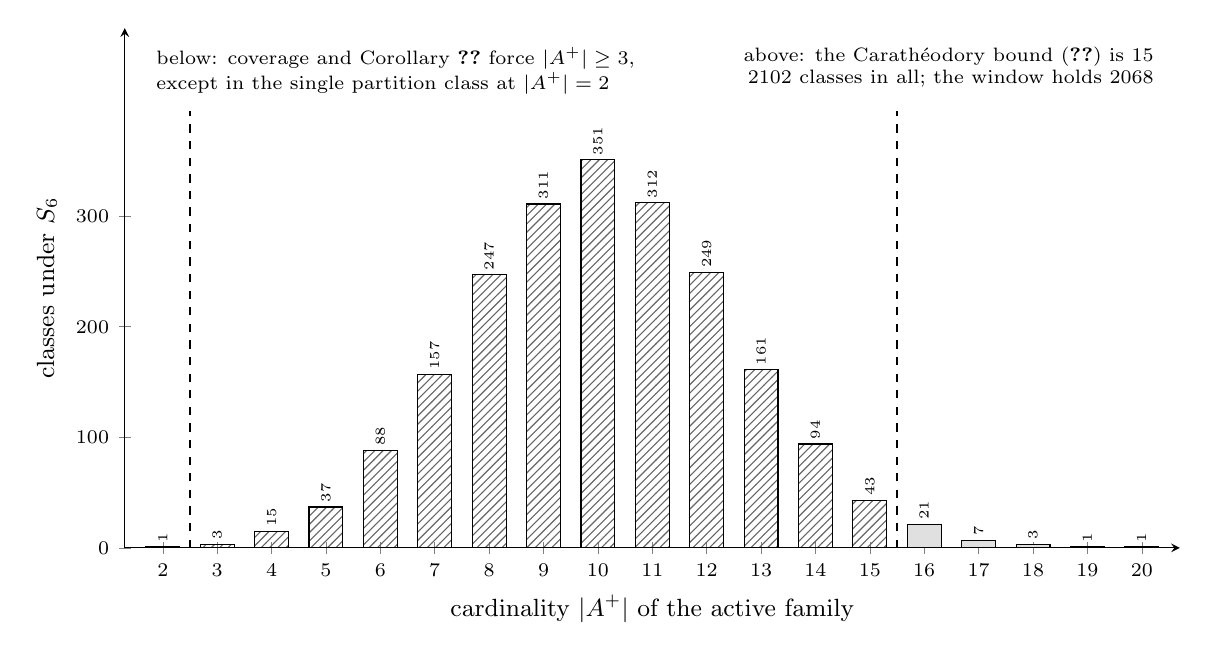
\begin{tikzpicture}
\begin{axis}[
  width=13.4cm, height=6.6cm,
  scale only axis,
  ybar, bar width=4.3mm,
  xmin=1.3, xmax=20.7,
  ymin=0, ymax=470,
  xtick={2,3,4,5,6,7,8,9,10,11,12,13,14,15,16,17,18,19,20},
  ytick={0,100,200,300},
  xlabel={cardinality $\lvert A^{+}\rvert$ of the active family},
  ylabel={classes under $S_6$},
  xlabel style={font=\small}, ylabel style={font=\small},
  tick label style={font=\scriptsize},
  axis lines=left,
  every axis plot/.append style={bar shift=0pt},
  nodes near coords,
  nodes near coords style={font=\tiny, rotate=90, anchor=west, inner sep=1.5pt},
  clip=false]

% ---- outside the window, below --------------------------------------
\addplot[draw=black, line width=0.4pt, fill=black!12]
  coordinates {(2,1)};

% ---- the window 3 <= |A| <= 15 --------------------------------------
\addplot[draw=black, line width=0.4pt,
         pattern=north east lines, pattern color=black!60]
  coordinates {(3,3) (4,15) (5,37) (6,88) (7,157) (8,247) (9,311)
               (10,351) (11,312) (12,249) (13,161) (14,94) (15,43)};

% ---- outside the window, above --------------------------------------
\addplot[draw=black, line width=0.4pt, fill=black!12]
  coordinates {(16,21) (17,7) (18,3) (19,1) (20,1)};

% ---- the cut-offs ----------------------------------------------------
\draw[dashed, line width=0.7pt] (axis cs:2.5,0) -- (axis cs:2.5,395);
\draw[dashed, line width=0.7pt] (axis cs:15.5,0) -- (axis cs:15.5,395);
\node[font=\scriptsize, anchor=north west, align=left]
  at (axis cs:1.7,462)
  {below: coverage and Corollary~\ref{cor:e3} force
   $\lvert A^{+}\rvert\ge3$,\\
   except in the single partition class at $\lvert A^{+}\rvert=2$};
\node[font=\scriptsize, anchor=north east, align=right]
  at (axis cs:20.4,462)
  {above: the Carath\'eodory bound \eqref{eq:carath} is $15$\\
   $2102$ classes in all; the window holds $2068$};
\end{axis}
\end{tikzpicture}

  \caption{The census of Proposition~\ref{prop:census} at $(6,3)$.  The
  active family covers $\{1,\dots,6\}$, so it has at least two members,
  and the one class of cardinality two is the partition that
  Corollary~\ref{cor:e3} leaves undecided; \eqref{eq:carath} removes the
  classes above fifteen.}
  \label{fig:census}
\end{figure}

\begin{conjecture}\label{conj:sixthree}
No design at $(6,3)$ carries an admissible stationarity datum with
$0<\cv<1$.
\end{conjecture}

\begin{conjecture}\label{conj:seventhree}
No design at $(7,3)$ carries an admissible stationarity datum with
$0<\cv<1$.
\end{conjecture}

Admissibility may not be dropped: Theorem~\ref{thm:reach} refutes the
corresponding statement at $(4,2)$ without it.  With it, each conjecture
is a finite conjunction of semialgebraic emptiness questions, one for
each of the classes counted in Proposition~\ref{prop:census}.  For a
fixed active family the unknowns are the $mk$ coordinates, the $m$
weights, the multipliers, the tight directions, the entries of $\Lambda$
and the value $\cv$; the conditions are \eqref{eq:statg},
\eqref{eq:statt}, $\lVert u_i\rVert=1$, $S_{C_i}u_i=\cv u_i$,
$\lambda_i\ge0$, $\sum_i\lambda_i=1$, \eqref{eq:parseval}, $t\pd0$,
$\sum_ct_c=1$, $0<\cv<1$, and \eqref{eq:argmax} --- the last a disjunction
of sign conditions on the leading principal minors of $\SC-\cv I$, one
disjunction for each $k$-subset $C$.

\begin{theorem}[conditional]\label{thm:rankthree}
Assume Conjectures~\ref{conj:sixthree} and~\ref{conj:seventhree}, and
assume that a failure of $\Gtz(6,3)$, respectively of $\Gtz(7,3)$,
produces an extremal counterexample at that cell in the sense of
Definition~\ref{def:extremalcex}.  Then $\Gtz(m,3)$ holds for every $m$.
\end{theorem}

\begin{proof}
By Corollary~\ref{cor:twocells} it suffices to prove $\Gtz(6,3)$ and
$\Gtz(7,3)$.  Suppose $\Gtz(6,3)$ fails.  By hypothesis $F$ attains a
local minimum over the designs at $(6,3)$ at a design of value $\cv<1$,
and $\cv>0$ by Lemma~\ref{lem:fpos}.  Theorem~\ref{thm:firstorder}
produces at that design a stationarity datum with value $\cv$, and it is
admissible because $\cv=F$ there.  This contradicts
Conjecture~\ref{conj:sixthree}.  The same argument at $(7,3)$ with
Conjecture~\ref{conj:seventhree} gives $\Gtz(7,3)$.
\end{proof}

The extremality hypothesis is all this section takes from
\S\ref{sec:compactness}; Theorem~\ref{thm:variational} supplies it for
the chart objective.

At $(6,3)$ the conjecture is an enumeration; at $(7,3)$ it is not, and an
argument uniform in the active family is required.  The exclusions of \S\ref{sec:exclusions} remove the small and the
transversal configurations, and Example~\ref{ex:splitseven} shows where the residue
lives: at the frontier size the system is realized, at the threshold, by
an active family of twenty triples.

\begin{wip}
Decide the partition branch of Corollary~\ref{cor:e3}: either exclude a
datum whose active family is a two-block partition of $\{1,\dots,6\}$
with $0<\cv<1$, or exhibit one.
\end{wip}

\section{Formalization}\label{sec:formalization}

The development is carried out in Lean~4 over Mathlib, and a statement
whose head carries the tag \emph{Lean} is verified there.
Tables~\ref{tab:lean} and~\ref{tab:leantwo} name the declaration behind
every tagged statement, and all of them where a statement is assembled from
several.  Three tags are not discharged in full, and \S\ref{sec:boundaries}
records which.

The formal statements are the originals, and the statements in the text
are their transcriptions.

\subsection{What is formalized}\label{sec:whatformal}

The formal definitions are those of \S\ref{sec:first} verbatim.  A design is a
structure carrying the vectors, the weights, positivity of the weights, their
normalization, and \eqref{eq:parseval}; domination of a subset is positive
semidefiniteness of $\SC-I$; and $\Gtz(m,k)$ is the assertion that every
design of size $m$ and rank $k$ admits a dominating subset of cardinality $k$.
No nondegeneracy is assumed: repeated atoms and zero atoms are admitted, and
the results of \S\ref{sec:ties} depend on that.

There is no separate real and complex development.  The structure and the
elementary theory are written once for scalars in an \texttt{RCLike} field
with real weights, and $\R$ and $\C$ are instantiations, definitionally so
over $\R$; Theorems~\ref{thm:corankone} and~\ref{thm:duality} and
Proposition~\ref{prop:sizerank} are proved at that generality and used at both.
Where a statement is genuinely field-dependent, as
Theorem~\ref{thm:complex} and Theorem~\ref{thm:ranktwo} are, it is
proved at the field where it holds.

The chart of
\S\ref{sec:chart} is formalized as the projection $P=VV\adj$ of
\eqref{eq:chart} together with the equivalence of Lemma~\ref{lem:chart}, and
the compactification of \S\ref{sec:compactness} as the predicate of
Definition~\ref{def:chartpoint} on pairs $(P,t)$ with $P$ a symmetric
idempotent of trace $k$ and $t$ in the closed simplex.  The stationarity
system of \S\ref{sec:interior} is a structure bundling
\eqref{eq:statg}--\eqref{eq:statt} with the active family and the
multipliers, and the results of that section are implications from it.

Graphic designs, used for the diamond of Example~\ref{ex:diamond}, are
formalized through \eqref{eq:graphicatom}.  The whitener is then an
existential and the atoms are determined only up to the orthogonal group,
so what is rational, and what the formal statements quantify over, is the
graph data.

\begin{table}[htbp]
\small
\begin{tabular}{@{}ll@{}}
\toprule
Statement & Declaration \\
\midrule
\multicolumn{2}{@{}l}{\emph{\S\ref{sec:first}, elementary cases}}\\
Lemma~\ref{lem:span}           & \texttt{Gtz.rank\_le\_size\_of\_fieldDesign}, \\
                               & \texttt{Gtz.eq\_zero\_of\_forall\_atom\_dot\_eq\_zero} \\
Lemma~\ref{lem:trace}          & \texttt{Gtz.trace\_identity} \\
Lemma~\ref{lem:share}          & \texttt{Gtz.weighted\_leverage\_le\_one} \\
Lemma~\ref{lem:coparseval}     & \texttt{Gtz.coParsevalOperator\_posDef} \\
Proposition~\ref{prop:sizerank}& \texttt{Gtz.gtzWeighted\_square} \\
Proposition~\ref{prop:rankone} & \texttt{Gtz.gtz\_rank\_one} \\
Proposition~\ref{prop:classical}
                               & \texttt{Gtz.gtzOriginal\_of\_projectionCovering}, \\
                               & \texttt{Gtz.gtzOriginal\_iff\_frameProjectionCovering} \\
Lemma~\ref{lem:direction}      & \texttt{Gtz.exists\_atom\_covering\_direction} \\
Example~\ref{ex:tetra}         & \texttt{Gtz.tetraDesign\_isTie} \\
\addlinespace
\multicolumn{2}{@{}l}{\emph{\S\ref{sec:chart}, the projection chart}}\\
Proposition~\ref{prop:chartid} & \texttt{Gtz.projectionChart\_diagonal},
                                 \texttt{Gtz.trace\_projectionChart} \\
Lemma~\ref{lem:congruence}     & \texttt{Gtz.chartBlock\_sub\_weightDiagonal} \\
Lemma~\ref{lem:flip}           & \texttt{Gtz.posSemidef\_one\_sub\_iff\_contraction}, \\
                               & \texttt{Gtz.contraction\_flip} \\
Lemma~\ref{lem:chart}          & \texttt{Gtz.fieldDominates\_iff\_posSemidef\_chartBlock\_finset} \\
Corollary~\ref{cor:minor}      & \texttt{Gtz.det\_projectionBlock\_sub\_weightDiagonal} \\
Lemma~\ref{lem:rayleigh}       & \texttt{Gtz.chartGapRayleigh\_pos\_of\_fixed}, \\
                               & \texttt{Gtz.chartGapRayleigh\_eq\_of\_killed} \\
Remark~\ref{rem:nogo}          & \texttt{Gtz.inertiaNoGoMatrix\_positive\_direction} and companions \\
Lemma~\ref{lem:whiten}         & \texttt{Gtz.exists\_congruence\_to\_one} \\
Theorem~\ref{thm:duality}      & \texttt{Gtz.weighted\_naimark\_duality} \\
Corollary~\ref{cor:dualcell}   & \texttt{Gtz.gtzWeighted\_dual\_iff} \\
Lemma~\ref{lem:rankone}        & \texttt{Gtz.posSemidef\_sub\_vecMulVec\_iff}, \\
                               & \texttt{Gtz.posDef\_sub\_vecMulVec\_iff} \\
Theorem~\ref{thm:corankone}    & \texttt{Gtz.corank\_one\_dominating\_erasure}, \\
                               & \texttt{Gtz.fieldGtzWeighted\_corank\_one},
                                 \texttt{Gtz.isTie\_iff\_forall\_pivot\_eq\_one}, \\
                               & \texttt{Gtz.exists\_realDesign\_exactlyTied},
                                 \texttt{Gtz.exists\_complexDesign\_exactlyTied} \\
\addlinespace
\multicolumn{2}{@{}l}{\emph{\S\ref{sec:complex}, the complex problem}}\\
Proposition~\ref{prop:cpositive}
                               & \texttt{Gtz.complexGtzWeighted\_square}, \\
                               & \texttt{Gtz.complexGtzWeighted\_corank\_one} \\
Example~\ref{ex:sic}           & \texttt{Gtz.sicParseval}, \texttt{Gtz.sicNorm} \\
Lemma~\ref{lem:sicvalue}       & \texttt{Gtz.sicDesign\_valueAtMost},
                                 \texttt{Gtz.pair\_not\_posSemidef} \\
Lemma~\ref{lem:spike}          & \texttt{Gtz.spikePaddedDesign\_valueAtMost} \\
Lemma~\ref{lem:split}          & \texttt{Gtz.splitAtomWeight\_valueAtMost} \\
Theorem~\ref{thm:ladder}       & \texttt{Gtz.complexRankConstantAtMostAtSize\_rank\_add} \\
Theorem~\ref{thm:complex}      & \texttt{Gtz.complexGtzWeighted\_iff\_size\_le\_rank\_add\_one} \\
\quad (negative half)          & \texttt{Gtz.not\_complexGtzWeighted\_of\_rank\_add\_two\_le\_size} \\
Example~\ref{ex:trine}         & \texttt{Gtz.trineBinding\_leastEigenvalue}, \\
                               & \texttt{Gtz.complexRankConstantAtMost\_three\_trine} \\
Example~\ref{ex:hesse}         & \texttt{Gtz.hesseAtom\_leverage},
                                 \texttt{Gtz.hesseAtom\_overlapCube} \\
Proposition~\ref{prop:hesse}   & \texttt{Gtz.hesseMargin\_isRoot},
                                 \texttt{Gtz.hesseDesign\_valueAtMost}, \\
                               & \texttt{Gtz.hesseMargin\_isGreatest} \\
\addlinespace
\multicolumn{2}{@{}l}{\emph{\S\ref{sec:real}, the decided real cells}}\\
Theorem~\ref{thm:light}        & \texttt{Gtz.dominating\_of\_light\_atom} \\
Corollary~\ref{cor:heavy}      & \texttt{Gtz.gtzWeightedAll\_of\_heavy} \\
Theorem~\ref{thm:ranktwo}      & \texttt{Gtz.gtz\_rank\_two} \\
Theorem~\ref{thm:coranktwo}    & \texttt{Gtz.gtzWeighted\_corank\_two} \\
Corollary~\ref{cor:corank}     & \texttt{Gtz.gtzWeighted\_of\_le\_five} \\
Lemma~\ref{lem:null}           & \texttt{Gtz.exists\_null\_direction} \\
Theorem~\ref{thm:reduce}       & \texttt{Gtz.exists\_reduced\_design} \\
Theorem~\ref{thm:window}       & \texttt{Gtz.crystallization} \\
Lemma~\ref{lem:repeat}         & \texttt{Gtz.not\_dominates\_of\_repeated\_atom} \\
Proposition~\ref{prop:splitting}& \texttt{Gtz.gtzWeighted\_of\_succ} \\
Theorem~\ref{thm:topcell}      & \texttt{Gtz.gtzWeightedAll\_of\_top}, \\
                               & \texttt{Gtz.gtz\_iff\_top\_of\_each\_rank} \\
Proposition~\ref{prop:spike}   & \texttt{Gtz.gtzWeighted\_of\_spike} \\
\bottomrule
\end{tabular}
\medskip
\caption{Correspondence between the numbered statements and the formal
development, first part: the elementary theory, the chart, the complex answer
and the decided real cells.}
\label{tab:lean}
\end{table}

\begin{table}[htbp]
\small
\begin{tabular}{@{}ll@{}}
\toprule
Statement & Declaration \\
\midrule
\multicolumn{2}{@{}l}{\emph{\S\ref{sec:ties}, the equality locus}}\\
Theorem~\ref{thm:tieseverywhere}& \texttt{Gtz.exists\_isTie\_of\_weights\_of\_classes}, \\
                               & \texttt{Gtz.splitClassDesign\_isTie},
                                 \texttt{Gtz.splitTetraDesign\_isTie}, \\
                               & \texttt{Gtz.splitSevenDesign\_isTie} \\
Example~\ref{ex:split}         & \texttt{Gtz.splitTetraDesign\_dominates}, \\
                               & \texttt{Gtz.splitTetraDesign\_no\_strictDominator} \\
Corollary~\ref{cor:nomargin}   & \texttt{Gtz.not\_exists\_card\_posSemidef\_sub\_smul\_one\_of\_isTie}, \\
                               & \texttt{Gtz.not\_gtzWeightedFloor\_rankThree\_of\_one\_lt} \\
Example~\ref{ex:diamond}       & \texttt{Gtz.diamondDesign\_isTie}$^{a}$, \\
                               & \texttt{Gtz.not\_hasParallelPair\_diamondDesign} \\
Corollary~\ref{cor:noparallel} & \texttt{Gtz.not\_hingeHoldsAtSize\_five\_three},
                                 \texttt{Gtz.diamondEdgeVector\_eq} \\
Theorem~\ref{thm:leverageaverage}
                               & \texttt{Gtz.posSemidef\_leverageWeightedAtomSum\_sub\_one} \\
Proposition~\ref{prop:jensen}  & \texttt{Gtz.sq\_rank\_le\_expectedElementary\_one} \\
Proposition~\ref{prop:qonezero}& \texttt{Gtz.mixedCharPoly\_eval\_one\_eq\_zero\_of\_totalTieSupported} \\
\addlinespace
\multicolumn{2}{@{}l}{\emph{\S\ref{sec:compactness}, the variational principle}}\\
Theorem~\ref{thm:boundary}     & \texttt{Gtz.exists\_chartDominates\_of\_weight\_eq\_zero} \\
Corollary~\ref{cor:interiorcex}& \texttt{Gtz.weight\_pos\_of\_forall\_not\_chartDominates} \\
Theorem~\ref{thm:sharp}        & \texttt{Gtz.not\_eventualCompressionLiftClaim} \\
\addlinespace
\multicolumn{2}{@{}l}{\emph{\S\ref{sec:interior}, interior critical points}}\\
Proposition~\ref{prop:quadric} & \texttt{Gtz.quadricLaw\_of\_isQuadricStationaryData}, \\
                               & \texttt{Gtz.coverageLaw\_of\_isQuadricStationaryData}, \\
                               & \texttt{Gtz.multiplierMatrix\_eq\_of\_isQuadricStationaryData} \\
Lemma~\ref{lem:overlap}        & \texttt{Gtz.tightOverlap\_sum\_eq\_one\_of\_isQuadricStationaryData}, \\
                               & \texttt{Gtz.one\_le\_leverage\_of\_isQuadricStationaryData}, \\
                               & \texttt{Gtz.exists\_rayleighProbe\_ge\_rank\_of\_isQuadricStationaryData}, \\
                               & \texttt{Gtz.exists\_mem\_activeSubset\_of\_isQuadricStationaryData} \\
Corollary~\ref{cor:singleactive}
                               & \texttt{Gtz.value\_eq\_rank\_of\_singleActive}, \\
                               & \texttt{Gtz.not\_isQuadricStationaryData\_of\_singleActive\_of\_value\_lt\_one} \\
Proposition~\ref{prop:saturated}& \texttt{Gtz.weight\_mul\_value\_eq\_one\_of\_saturatedAtom}, \\
                               & \texttt{Gtz.one\_le\_value\_of\_saturatedAtom} \\
\addlinespace
\multicolumn{2}{@{}l}{\emph{Appendix~\ref{app:graveyard}, excluded strategies}}\\
Proposition~\ref{prop:noaggregate}
                               & \texttt{Gtz.not\_hasUniformTieAggregateSeven}, \\
                               & \texttt{Gtz.splitSevenDesign\_weightedTieAggregate\_nonpos}, \\
                               & \texttt{Gtz.closedTieFailure\_inhabited\_seven} \\
Proposition~\ref{prop:twomoment}& \texttt{Gtz.dominates\_of\_twoMomentGap\_nonneg} \\
Proposition~\ref{prop:icosa}   & \texttt{Gtz.icosa\_twoMomentGap\_eq},
                                 \texttt{Gtz.icosa\_no\_twoMoment\_certificate}, \\
                               & \texttt{Gtz.icosaDesign\_strictly\_dominates} \\
\bottomrule
\end{tabular}
\medskip
\caption{Correspondence, second part: the equality locus, the variational
principle, the interior system and the excluded strategies.  The declaration
marked $a$ is proved but does not appear in the axiom ledger described in
\S\ref{sec:axioms}.}
\label{tab:leantwo}
\end{table}

\subsection{Axiom discipline}\label{sec:axioms}

A ledger module lists, for the declarations of the development, the axioms on
which each depends, printed by the kernel rather than asserted by the author.
The permitted set is Mathlib's
$\{\texttt{propext},\ \texttt{Classical.choice},\ \texttt{Quot.sound}\}$, and
nothing outside it occurs.  Classical logic is used freely, and nothing in
the development is a constructive claim.

In particular no declaration depends on \texttt{sorryAx}: the development
contains no incomplete proof.  It contains no \texttt{axiom} declaration.
Closed arithmetic over concrete finite index sets is discharged by kernel
evaluation of decidable propositions, which introduces no axiom.  No proof
is closed by compiled evaluation.

The ledger covers exactly what it lists: one
declaration, the entry marked $a$ in Table~\ref{tab:leantwo}, is absent
from it, and is proved in a module duplicating
one that the ledger does cover.  Its proof is checked when that module is
elaborated, but its axiom use is not certified by the ledger.

No numerical assertion in the paper rests on floating-point evaluation.  The
witnesses of \S\ref{sec:sharp} and Appendix~\ref{app:graveyard} are exact
rationals in the formal statements and are checked as such; the icosahedral and
graphic designs of Appendix~\ref{app:data} carry radicals, and the
formal statements use the algebraic relations \eqref{eq:icosaconst} and
\eqref{eq:graphicleverage} that eliminate them.  Remark~\ref{rem:hygiene} records the
conditioning phenomenon that makes this discipline necessary rather than
decorative.

\subsection{Where the formalization stops}\label{sec:boundaries}

Two steps of the argument are not formal.  Both lie in
\S\ref{sec:compactness}--\S\ref{sec:interior}.

The first is the attainment in Theorem~\ref{thm:variational}: a continuous
function on a compact space attains its minimum.  The space of chart points is
compact --- a product of a Grassmannian and a closed simplex --- and the
objective $G$ of Definition~\ref{def:chartpoint} is continuous, being a maximum
of finitely many least-eigenvalue functions of continuous matrix-valued maps.
We use this standard fact without formalizing it.  Its two nontrivial
inputs, Theorem~\ref{thm:boundary} and Corollary~\ref{cor:interiorcex},
which place the minimizer at a design rather than at a boundary point,
are formal.

The second is the passage from a local minimum to the system
\eqref{eq:statg}--\eqref{eq:statt}.  Its ingredients are the spectraplex,
the composition rule and the maximum rule, assembled in \S\ref{sec:kkt};
each is classical
\cite{Danskin1967,Overton1988,HiriartUrrutyYe1995,Clarke1990} and none is
in the ambient library.  So \S\ref{sec:interior} takes the system as its
hypothesis and formalizes its consequences
(Proposition~\ref{prop:quadric}, Proposition~\ref{prop:e1} and the
exclusions) rather than deriving the system from minimality.

The two conjectural inputs of Theorem~\ref{thm:rankthree} speak about the
system, not about minimality, so a proof of either closes the corresponding
cell only together with the two steps above.

Three tags are narrower than the statement they head, and in each case the
gap is one step of the printed proof.
\begin{enumerate}
\item[\rm(i)] Proposition~\ref{prop:rankfloor} is stated over $\FF$ and
  formalized over $\R$, as\\
  \texttt{Gtz.gtzWeightedFloor\_inv\_rank}.  Its proof does not consult the
  field, so the complex case is a transcription and not a mathematical gap.
\item[\rm(ii)] In Proposition~\ref{prop:tielawcorank} the per-atom
  equivalence is formal, as\\
  \texttt{Gtz.jensenRatio\_eq\_inv\_rank\_iff\_leverageIdentity},\\
  and the summation that concludes $m=k+1$ is not.
\item[\rm(iii)] In Lemma~\ref{lem:defect} the two consequences drawn from the
  identity are formal, as\\
  \texttt{Gtz.weight\_mul\_value\_le\_one\_of\_isQuadricStationaryData} and\\
  \texttt{Gtz.weight\_mul\_value\_eq\_one\_of\_saturatedAtom};\\
  the identity itself, one subtraction of \eqref{eq:coverage} from
  \eqref{eq:overlapone}, is not stated on its own.
\end{enumerate}

\section{Problems}\label{sec:open}

Problems~\ref{prob:sixthree} and~\ref{prob:seventhree} together decide the
real problem at rank three, by Theorem~\ref{thm:rankthree}.

\begin{enumerate}

\item\label{prob:sixthree}
\emph{Prove Conjecture~\ref{conj:sixthree}: the stationarity system
\eqref{eq:statg}--\eqref{eq:statt} has no admissible solution at $(6,3)$ with
$0<\cv<1$.}

Such a proof closes $\Gtz(6,3)$ through Theorem~\ref{thm:rankthree}, which also
assumes that the cell has a minimizing counterexample
(Definition~\ref{def:extremalcex}).  Theorem~\ref{thm:variational} supplies that
assumption for the chart objective, on the two instances $\Gtz(5,3)$ and
$\Gtz(5,2)$ of Corollary~\ref{cor:corank}; by Remark~\ref{rem:objectives} a
minimizer of the chart objective need not minimize the design objective, and
nothing in the paper closes that gap.

The question is finite.  The active family $A^{+}$ covers the six
indices by \eqref{eq:coverage}, so it is one of the $2102$ families counted
in Proposition~\ref{prop:census}.  It has at least three members except in the
two-triple partition branch that Corollary~\ref{cor:e3} leaves undecided, and
setting that class aside leaves $2101$; it may be taken of cardinality
at most $15$ by Carath\'eodory's theorem \cite{Caratheodory1911}
(Proposition~\ref{prop:carath}), which leaves $2068$ (\S\ref{app:census}).  The
exclusions of \S\ref{sec:exclusions} settle $57$ classes of the full census of
$2136$, and the remainder is concentrated where they are silent.  For each class
the task is to show that \eqref{eq:statg}, \eqref{eq:statt}, the eigenvector
equations $S_{C_i}u_i=\cv u_i$, \eqref{eq:parseval} and the admissibility
disjunction \eqref{eq:argmax} have no common real solution with every
$t_c>0$, every $\lambda_i\ge0$ and $0<\cv<1$.

Any elimination must respect the system's multiplicities and its redundancy.  If
$\cv$ is an eigenvalue of $\SC$ of multiplicity $r$ at an active $C$, then the
multiplier attached to $C$ is a positive semidefinite matrix of trace one on
that eigenspace \eqref{eq:spectraplex}, and $C$ carries up to $r$ of the indices
of $A$ rather than one.  And \eqref{eq:coverage} is \eqref{eq:statg} contracted,
with $\mu=\cv$ following from it, so the constraints must not be counted as
independent.

\item\label{prob:seventhree}
\emph{Prove Conjecture~\ref{conj:seventhree}: the same at $(7,3)$.}

With Problem~\ref{prob:sixthree} this decides the real problem at rank three,
by Theorem~\ref{thm:rankthree}.  Enumeration is not available: the census has
$7\,011\,184$ classes, of which $5\,249\,381$ lie within the Carath\'eodory
bound $19$ (\S\ref{app:census}).  An argument uniform in the active family is
wanted, one using only the laws \eqref{eq:statt} and \eqref{eq:coverage}, the
positivity of the weights, and the combinatorics of a covering family, never
the family's identity.

The split tetrahedra of \S\ref{app:split} have value $\cv=1$ at this cell, and
their active family is the set of triples meeting three distinct classes, so its
cardinality is the third elementary symmetric function of the class sizes: $13$,
$17$ and $20$ at the profiles $(4,1,1,1)$, $(3,2,1,1)$ and $(2,2,2,1)$.  A
uniform argument must therefore exclude $\cv<1$ without excluding any of the
three.

\item\label{prob:sharpc}
\emph{Determine $\alpha_3(\C)$.}

Remark~\ref{rem:sharpc} gives
$\tfrac13\le\alpha_3(\C)\le3\bigl(1-\cos\tfrac{2\pi}{9}\bigr)=0.7018\ldots$,
the upper bound realized by a binding triple of the Hesse configuration of nine
equiangular lines in $\C^3$.  We conjecture that the upper bound is the truth.
At $k=2$ both ends meet, $\alpha_2(\C)=2-2/\sqrt3$; for $k\ge3$ the two ends of
\S\ref{sec:csharp} are all that is known.  Over $\R$ the same question is empty
below rank three and, if Problems~\ref{prob:sixthree}
and~\ref{prob:seventhree} go as conjectured, empty at rank three, so it first
has content at $\alpha_4(\R)$.

\item\label{prob:interlace}
\emph{Derandomize Theorem~\ref{thm:average}.}

Volume sampling \cite{DRVW2006} assigns $\pi_C=\det P[C]$ to a $k$-subset by
\eqref{eq:dpp}.  The measure is determinantal, carried by the bases of the
underlying matroid \cite{Lyons2003}, and it is strongly Rayleigh
\cite{BorceaBrandenLiggett2009}, so the mixture $q=\E_\pi[\chi_{\SC}]$ is
real-rooted \cite{AnariOveisGharan2015}.  Two statements would together prove
$\Gtz(m,k)$ at every rank at once:
\begin{enumerate}
\item[(a)] some $k$-subset $C$ has $\lmin(\SC)$ at least the least root of $q$;
\item[(b)] that least root is at least $1$.
\end{enumerate}

Neither is available.  Statement (a) does not follow from real-rootedness of
$q$ alone (Proposition~\ref{prop:rootedness}), and the interlacing method of
\cite{MSS2015} requires the whole convex family to be real-rooted, a property
of volume sampling that has not been verified.  Statement (b) must be exact
on the equality locus, by Proposition~\ref{prop:qone}: at a design where
every basis has $1$ in the spectrum of $\SC$ one has $q(1)=0$, with no
margin, and at the tetrahedron $q=(x-1)(x-4)^2$ (\S\ref{app:tetra}).

A route through this problem would be the first argument in the subject that
does not proceed cell by cell.  Nothing in this paper manages that.

\item\label{prob:structure}
\emph{Classify the extremal designs.}

Theorem~\ref{thm:corankone} classifies them at corank one: over each weight
vector there is one, given in \S\ref{app:corankone}, and \eqref{eq:tielaw} is a
complete description.  Beyond corank one the constructed families are the
split-class designs of \S\ref{app:split}, which have at most $k+1$ distinct
directions, and the splittings of the diamond of \S\ref{app:diamond}, which
has $k+2$.

Is that list complete at $(6,3)$ and $(7,3)$?  Is it finite, as a list of
families?  Does every extremal design have every basis active, that is
$\lmin(\SC)=1$ for every independent $k$-subset $C$?
Every known extremal design does: at the tetrahedron all four
triples are bases and all are active, and at the diamond the eight spanning
trees are bases and all eight have positive semidefinite singular gaps, the two
circuits being dependent and carrying no volume-sampling mass.  An affirmative
answer gives the hypothesis under which Proposition~\ref{prop:qone}
yields $q(1)=0$, and so is what Problem~\ref{prob:interlace} would have to
face at the equality locus.

\item\label{prob:higher}
\emph{Determine the true window in Theorem~\ref{thm:window}.}

Nothing in the proof of Lemma~\ref{lem:null}
refers to domination, so no lower bound on the window follows from it.  At
$k=2$ the
problem is decided at every size by Theorem~\ref{thm:ranktwo}, so the window is
vacuous there; at $k=3$ the bound is $7$ and the two cells $(6,3)$ and $(7,3)$
survive.  Is the window ever larger than $k+3$?  Equivalently: is there a rank
$k$ and a size $m>k+3$ at which $\Gtz(m,k)$ is strictly harder than at every
smaller size?  Corollary~\ref{cor:corank} settles corank at most two, so the
question is first posed at corank three.

\item\label{prob:effective}
\emph{Find the subset.}

The selection principle asserts that a subset exists; neither known route
exhibits one.  Volume sampling dominates only on average
(Theorem~\ref{thm:average}).  The maximal-volume principle
\cite{GT2001} does name a subset, and the guarantee it comes with is too
weak.  At uniform
weights that principle bounds a locally maximal-volume choice by
$\lVert A_C^{-1}\rVert^2\le1+k(m-k)$ for the matrix $A$ of rows $u_c=g_c/\sqrt m$,
which in the normalization of \eqref{eq:dominate} reads
\[
  \lmin(\SC)\;\ge\;\frac{m}{1+k(m-k)} .
\]
By \eqref{eq:deficit} the right side equals $1$ exactly when $k=1$ or $m=k+1$
and is strictly smaller otherwise, so the principle reproduces
Theorem~\ref{thm:corankone} and nothing beyond it.

Computing a maximal-volume subset is itself out of reach: the problem is
NP-hard and NP-hard to approximate within a constant factor
\cite{CivrilMagdonIsmail2009}, and the rank-revealing factorizations that
approximate it \cite{GuEisenstat1996} inherit the weaker guarantee.

The witnesses named below are Lean declarations, verified and covered by
the ledger of \S\ref{sec:axioms}.

At general weights the rule fails outright.  The volume of $C$ is $\pi_C$ of
\eqref{eq:dpp}; at a design at $(7,3)$ whose atom vectors are integral, whose
weights are integer multiples of $\tfrac1{60}$ and whose leverages are all at
least $2$, the maximum of $\pi_C$ over the thirty-five triples is attained at a
triple that does not dominate
(\texttt{Gtz.shadowDeterminant\_\allowbreak le\_\allowbreak shadowArgmaxSubset},
\texttt{Gtz.shadowArgmaxSubset\_\allowbreak not\_\allowbreak dominates}), while
another triple does
(\texttt{Gtz.shadowArgmaxDesign\_\allowbreak hasDominatingSubset}).  At that same design the
maximizer of the unweighted volume $\lvert\det M_C\rvert$ dominates strictly, so
what breaks the rule is the weighting by $\prod_{c\in C}t_c$ in \eqref{eq:dpp},
and Proposition~\ref{prop:rankfloor}, whose subset is the unweighted maximizer,
is untouched.

Whatever exhibits the subset must read the atom labels.  No triple dominates at
every design at $(6,3)$: two rational designs there each have a dominating
triple and share none
(\texttt{Gtz.no\_\allowbreak universal\_\allowbreak dominating\_\allowbreak subset},
\texttt{Gtz.exists\_\allowbreak designs\_\allowbreak with\_\allowbreak disjoint\_\allowbreak dominationSets}).  Invariant data
is not enough either: some design at $(6,3)$ is fixed atom-for-atom and
weight-for-weight by a nontrivial relabelling of its indices, has a dominating
triple, and has none that the relabelling fixes
(\texttt{Gtz.exists\_\allowbreak symmetry\_\allowbreak with\_\allowbreak no\_\allowbreak fixed\_\allowbreak dominatingSubset}), so every
rule computed from relabelling-invariant data fails there.  That witness is the
$(6,3)$ split tetrahedron of \S\ref{app:split} at $a=b=\tfrac18$, the
relabelling exchanging the two copies in each split direction, so the
obstruction sits on the equality locus.  Taking the atom of greatest leverage
fails at a design all of whose leverages exceed $1$
(\texttt{Gtz.heaviest\_\allowbreak atom\_\allowbreak can\_\allowbreak lie\_\allowbreak outside\_\allowbreak every\_\allowbreak dominatingSubset},
\texttt{Gtz.heavyPivotDesign\_\allowbreak allHeavy}).
Maximizing $\lmin(\SC)$ is not refuted and cannot be: its argmax dominates
whenever any triple does, and computing that argmax is the exhaustive search.

Local search is refuted at a bounded exchange radius.  Suppose a score has the
property that at every non-dominating $k$-subset some $k$-subset within $r$
swaps scores strictly higher; a finite argmax then proves $\Gtz(m,k)$.  At rank
three and $r\le2$ the property fails on all-heavy designs for $\lmin(\SC)$ at
both open cells, and at $(7,3)$ for the clipped trace, the trace of $\SC$ with
each eigenvalue replaced by its minimum with $1$, and for $\pi_C$
(\texttt{Gtz.not\_\allowbreak exchangeImprovesWithinRadiusHeavy\_\allowbreak of\_\allowbreak le\_\allowbreak two\_\allowbreak rankThree},
\texttt{Gtz.boundedRadiusExchangeHeavy\_\allowbreak refuted\_\allowbreak sevenThree}).  At $r=k$ the
radius constraint is vacuous.  The first two scores separate dominating from
failing subsets by a threshold, so at that radius their hypothesis is
$\Gtz(m,k)$ verbatim; for $\pi_C$ it is false with no radius bound at all.
Every witness above satisfies $\Gtz$ at its own cell.

Two questions therefore stand apart from the conjecture itself: does a subset of
maximal volume dominate at uniform weights, and, granting $\Gtz(m,k)$, is there
an algorithm polynomial in $m$ and $k$ that exhibits a dominating subset?

\end{enumerate}


\appendix
\section{Strategies excluded, with witnesses}\label{app:graveyard}

By Corollary~\ref{cor:nomargin} the selection inequality
\eqref{eq:dominate} is an equality on a set of full dimension in the
weights.  A device whose output is a strictly positive quantity therefore
asserts something false at every point of that set.  Four of the seven
strategies below fail for that reason alone.

For a $k$-subset $C$ of a design write $\Gram_C$ for the Gram matrix
$(\langle g_c,g_d\rangle)_{c,d\in C}$.  By \eqref{eq:twoproducts},
$\Gram_C=M_C^{\vphantom{\mathsf{H}}}M_C\adj$ and
$\SC=M_C\adj M_C^{\vphantom{\mathsf{H}}}$ with
$M_C$ square, so the two have the same spectrum and
\begin{equation}\label{eq:tieleg}
  \delta(C)\;:=\;\det\bigl(\Gram_C-I_k\bigr)\;=\;\det\bigl(\SC-I_k\bigr) .
\end{equation}
Domination of $C$ implies $\delta(C)\ge0$; we call $\delta$ the
\emph{determinant leg}.  At rank three we also use
\begin{equation}\label{eq:twomoment}
  \gamma(C)\;:=\;4\det\Gram_C-\bigl(\tr\Gram_C-1\bigr)^2 ,
\end{equation}
a function of the first two moments of the spectrum of $\SC$ alone.

\subsection{Certificates with a uniform floor}\label{app:certificates}

The natural request is a nonnegative combination of the determinant legs,
at each design, bounded below by a positive constant.  No such
combination exists, and the obstruction has nothing to do with degree,
polynomiality or equivariance: the coefficients below may be arbitrary
nonnegative functions of the design.

\begin{proposition}[Lean]\label{prop:noaggregate}
There is no $\theta>0$ with the following property: for every design $\dsn$ at
$(7,3)$ with $\ell_c>1$ for all $c$ there are numbers $w_C(\dsn)\ge0$, indexed by
the $35$ triples, with
\[
  \sum_{\lvert C\rvert=3} w_C(\dsn)\,\delta(C)\;\ge\;\theta .
\]
\end{proposition}

\begin{proof}
Let $\dsn_{\triangle}$ be the split tetrahedron at $(7,3)$ of \S\ref{app:split}: seven
atoms carrying the four tetrahedron directions with multiplicities $2,2,2,1$
and weights $(\tfrac18,\tfrac18,\tfrac18,\tfrac14,\tfrac18,\tfrac18,\tfrac18)$.
Every leverage equals $3$, so $\dsn_{\triangle}$ lies in the stated class.  A triple of
$\dsn_{\triangle}$ carries either three distinct directions or two equal ones.  In the
first case $\Gram_C$ has diagonal $3$ and off-diagonal $-1$, so
$\Gram_C-I_3=3I_3-J_3$, of eigenvalues $0,3,3$ and determinant $0$.  In the
second, after ordering so that the first two atoms agree,
\[
  \Gram_C-I_3=\begin{pmatrix}2&3&-1\\ 3&2&-1\\ -1&-1&2\end{pmatrix},
  \qquad \det=2(4-1)-3(6-1)+(-1)(-3+2)=-8 .
\]
Hence $\delta(C)\le0$ for all $35$ triples, and every nonnegative combination
of the legs at $\dsn_{\triangle}$ is at most $0$.
\end{proof}

Any Positivstellensatz certificate in Putinar or Schmüdgen form yields, on
evaluation at a design, exactly such a combination, its coefficients being the
sums of squares evaluated there and its floor the constant of the
representation.  So:

\begin{corollary}\label{cor:noputinar}
No representation
$\sum_{C}\sigma_C\,\delta(C)=1+\sigma_0$, valid on the all-heavy locus at
$(7,3)$ with $\sigma_0$ and the $\sigma_C$ nonnegative there, exists --- at any
degree.
\end{corollary}

\begin{proof}
Evaluate at $\dsn_{\triangle}$: the left side is at most $0$ and the right side at least
$1$.
\end{proof}

Consider the two systems on the all-heavy locus,
\[
  \text{(strict)}\quad \delta(C)<0 \ \ \text{for all } C,
  \qquad\qquad
  \text{(closed)}\quad \delta(C)\le0 \ \ \text{for all } C .
\]
Failure of $\Gtz(7,3)$ would give a point of the strict system; the design
$\dsn_{\triangle}$ is a point of the closed one.  So the closed system is
inhabited and carries no certificate of emptiness of any kind, while the
strict system is the one that must be certified empty.  The two systems
differ on the equality locus, and nowhere else.

\begin{remark}\label{rem:stengle}
Stengle's form, in which the multiplicative monoid part is nonempty,
survives; one can bound its size.  A Stengle certificate of emptiness of
the strict system is an identity $f+g^2+h=0$ with $f$ in the cone generated by
the defining inequalities, $h$ in the ideal generated by the equations, and
$g$ a product of powers of the strict generators $-\delta(C)$.  At any point of
the closed system all generators are nonnegative, so $f\ge0$ and $h=0$ there,
forcing $g=0$.  Now the closed system contains one split tetrahedron for each
partition of the seven indices into classes of sizes $2,2,2,1$, of which there
are $7!/(2!^3\,3!)=105$; at the partition $\Pi$ the leg $\delta$ vanishes
exactly on the $20$ triples meeting three distinct classes of $\Pi$.  So the set
of triples occurring as factors of $g$ must meet, for each of the $105$
partitions, that partition's own family of $20$.  No set of at most three
triples meets all $105$ families; $5355$ sets of four do, among them
$\{123,124,135,145\}$.  Since $\delta$
has degree $3$ in the entries of $\Gamma$ and degree $6$ in the atom
coordinates, the monoid part of every Stengle certificate has degree at least
$12$ in the $28$ Gram entries and at least $24$ in the $21$ coordinates.  A sum
of squares of degree $12$ in $28$ variables has a half-degree monomial basis of
$\binom{34}{6}=1\,344\,904$ elements.
\end{remark}

\subsection{Margin transfer across a deletion}\label{app:transfer}

Induction on the size deletes an atom, applies $\Gtz(m-1,k)$, and lifts.
The lift is exact, and one computation settles what it costs.

Let $\dsn$ be a design at $(m,k)$ and $e$ an index with $s_e<1$, equivalently
$I-t_e\,g_e^{\vphantom{\mathsf{T}}}g_e\tp\pd0$.  Choose $R$ with
$R\tp\bigl(I-t_e g_e^{\vphantom{\mathsf{T}}}g_e\tp\bigr)R=I$ and set
\[
  g'_c:=\sqrt{1-t_e}\;R\tp g_c,
  \qquad
  t'_c:=\frac{t_c}{1-t_e}
  \qquad (c\ne e).
\]
The weights are positive and sum to one, and
\[
  \sum_{c\ne e}t'_c\,g'^{\vphantom{\mathsf{T}}}_c{g'_c}\tp
  =R\tp\Bigl(\sum_{c\ne e}t_c\,g_c^{\vphantom{\mathsf{T}}}g_c\tp\Bigr)R
  =R\tp\bigl(I-t_e g_e^{\vphantom{\mathsf{T}}}g_e\tp\bigr)R=I,
\]
so $\dsn'$ is a design at $(m-1,k)$.

\begin{proposition}\label{prop:deletionprice}
Let $C\subseteq\{c:c\ne e\}$ have $\lvert C\rvert=k$ and satisfy
$S'_C\psd(1+\varepsilon)I$ in $\dsn'$, with $\varepsilon\ge0$.  Then $C$
dominates in $\dsn$ provided
\begin{equation}\label{eq:kappa}
  1+\varepsilon\;\ge\;\kappa_e^{-1},
  \qquad\text{where}\qquad
  \kappa_e:=\frac{1-s_e}{1-t_e} ,
\end{equation}
that is provided $\varepsilon\ge t_e(\ell_e-1)/(1-s_e)$.  The threshold is at
most $0$ if and only if $\ell_e\le1$.
\end{proposition}

\begin{proof}
From $R\tp\bigl(I-t_eg_e^{\vphantom{\mathsf{T}}}g_e\tp\bigr)R=I$ one reads
$RR\tp=\bigl(I-t_eg_e^{\vphantom{\mathsf{T}}}g_e\tp\bigr)^{-1}$, hence for
$y:=R^{-1}w$,
\[
  y\tp S'_Cy=(1-t_e)\,w\tp S_Cw,
  \qquad
  y\tp y=w\tp\bigl(I-t_eg_e^{\vphantom{\mathsf{T}}}g_e\tp\bigr)w
        =\lVert w\rVert^2-t_e\langle g_e,w\rangle^2 ,
\]
the first because $S'_C=(1-t_e)R\tp S_CR$.  Applying the hypothesis at $y$ and
taking $\lVert w\rVert=1$,
\[
  w\tp S_Cw\;\ge\;\frac{(1+\varepsilon)\bigl(1-t_e\langle g_e,w\rangle^2\bigr)}
                       {1-t_e}
   \;\ge\;\frac{(1+\varepsilon)(1-s_e)}{1-t_e}
   \;=\;(1+\varepsilon)\,\kappa_e ,
\]
by Cauchy--Schwarz, which gives $\langle g_e,w\rangle^2\le\ell_e$ and hence
$t_e\langle g_e,w\rangle^2\le t_e\ell_e=s_e$.  This is at least $1$
exactly under \eqref{eq:kappa}.  Finally
$\kappa_e^{-1}-1=(s_e-t_e)/(1-s_e)=t_e(\ell_e-1)/(1-s_e)$, whose sign is that
of $\ell_e-1$.
\end{proof}

Proposition~\ref{prop:deletionprice} is an identity, and it splits the
induction into the two branches already in use.  At $\ell_e\le1$
the threshold is nonpositive and the deletion needs nothing downstairs;
this is the light-atom step that reduces $\Gtz(m,k)$ to all-heavy
designs.  At $\ell_e>1$ the threshold is strictly positive.

\begin{corollary}\label{cor:noheavydeletion}
At rank three no deletion of a heavy atom transports domination without a
margin, and no such margin is available: by Corollary~\ref{cor:nomargin}, for
every $m\ge5$ and every $\varepsilon>0$ there is a design at $(m-1,3)$ with no
$k$-subset satisfying $\SC\psd(1+\varepsilon)I$.
\end{corollary}

No choice of the deleted atom repairs this, because the threshold depends on
$e$ only through $\ell_e$ and by Lemma~\ref{lem:trace} some atom has
$\ell_e\ge k$.

\subsection{Restricting the region}\label{app:region}

Cutting the degenerate part out of the design space and running a
compactness argument on the rest requires a cut that misses the equality
locus.  The two cuts that suggest themselves, a floor on the weights and
the exclusion of parallel atoms, both leave the locus intact.

By Theorem~\ref{thm:tieseverywhere} every weight vector on $m\ge k+1$ indices
carries an extremal design, one for each partition of the indices into $k+1$
nonempty classes; the construction is displayed in \S\ref{app:split}.  So no
restriction of the weight simplex --- to a compact subset, to a
neighbourhood of the uniform point, to any nonempty relatively open set ---
excludes the equality locus, and the infimum of the selection objective over
any such region is at most $1$.

The second cut fails for a different reason.  Every design produced by
splitting has two parallel atoms, so excluding parallel pairs removes the
constructed part of the equality locus.  It does not remove all of it: the
diamond of Example~\ref{ex:diamond}, whose data is in \S\ref{app:diamond}, is
an extremal design at $(5,3)$ whose five atoms are pairwise non-parallel.  Its
splittings give extremal designs with a parallel pair at $(6,3)$ and $(7,3)$,
and perturbing a split pair apart moves the design off the parallel locus while
moving the value by an arbitrarily small amount, since the value is continuous.

\subsection{The compression lift at positive weight}\label{app:lift}

The lift \eqref{eq:schur} used in Theorem~\ref{thm:boundary} holds at $t_z=0$
by an exact identity and fails at every positive $t_z$, however small
(Theorem~\ref{thm:sharp}).  The witness is the chart point and one-parameter
weight family of \S\ref{app:liftfail}, whose relevant $2\times2$ block has
determinant $-\tau(2+3\tau)/9$ at pivot weight $\tau$.  The failure is not a
matter of size: the deficit is of first order in $\tau$ against a downstairs
slack which the family freezes at $0$.  This is again
Corollary~\ref{cor:nomargin}, so the boundary analysis of
\S\ref{sec:boundary} runs at the limit point.

\subsection{Real-rootedness of the mixture}\label{app:rooted}

Theorem~\ref{thm:average} makes the selection problem a derandomization:
$\E_\pi[\SC]\psd I$, and one wants a single $C$.  The interlacing method
supplies derandomizations of just this shape, and the mixture
$q=\E_\pi[\chi_{\SC}]$ of Proposition~\ref{prop:qone} is the object it
would act on.  Real-rootedness of $q$ alone, however, buys nothing.

\begin{proposition}\label{prop:rootedness}
There are real-rooted monic quadratics $f_1,f_2$ whose average is real-rooted
and whose average has least root strictly larger than the least roots of both.
\end{proposition}

\begin{proof}
Take
\[
  f_1=X^2-X,\qquad f_2=X^2-23X+60,
\]
with roots $\{0,1\}$ and $\{3,20\}$, so least roots $0$ and $3$.  Their average
is $X^2-12X+30$, of discriminant $144-120=24>0$, with roots $6\pm\sqrt6$; the
least is $6-\sqrt6=3.5505\ldots>3$.
\end{proof}

The hypothesis the interlacing method actually requires is that the whole
convex family be real-rooted --- a common interlacing --- and the pair above
fails it:
\[
  \lambda f_1+(1-\lambda)f_2=X^2+(22\lambda-23)X+60(1-\lambda),
  \qquad
  \operatorname{disc}=484\lambda^2-772\lambda+289 ,
\]
which at $\lambda=\tfrac45$ equals $-\tfrac{471}{25}<0$.  So the conclusion of
\cite{MSS2015} is unavailable for this pair, and no contradiction
arises.  Nor is real-rootedness
preserved by averaging in general: $X^2-1$ and $X^2+10X+25$ are real-rooted and
their average $X^2+5X+12$ has discriminant $-23$.  A derandomization of
Theorem~\ref{thm:average} must therefore verify the interlacing hypothesis for
volume sampling, not assume real-rootedness of the mixture.  This is
Problem~\ref{prob:interlace}.

\subsection{Two moments}\label{app:moments}

At rank three there is a genuine criterion in the first two moments of the
spectrum.  It is sharp among such criteria, and it does not decide the open
cells.

\begin{proposition}[Lean]\label{prop:twomoment}
Let $C$ be a $3$-subset of a design at rank three with
$\ell_C:=\tr\Gram_C>3$.  If $\gamma(C)\ge0$ then $C$ dominates.
\end{proposition}

\begin{proof}
Let $x\le y\le z$ be the eigenvalues of $\SC$, all nonnegative, with
$x+y+z=\ell_C$ and $xyz=\det\Gram_C$.  By the arithmetic--geometric mean
inequality applied to $y,z$,
\[
  4\det\Gram_C=4xyz\le 4x\Bigl(\frac{y+z}{2}\Bigr)^2=x(\ell_C-x)^2 .
\]
The hypothesis $\gamma(C)\ge0$ reads $4\det\Gram_C\ge(\ell_C-1)^2$, so
$x(\ell_C-x)^2-(\ell_C-1)^2\ge0$.  Expanding both sides,
\[
  x(\ell_C-x)^2-(\ell_C-1)^2=(x-1)\bigl(x^2+(1-2\ell_C)x+(\ell_C-1)^2\bigr),
\]
an identity in $x$ and $\ell_C$.  Write $Q(x)$ for the quadratic factor.  Its vertex
is at $x=\ell_C-\tfrac12>1$, so $Q$ decreases on $[0,1]$, and
$Q(1)=2-2\ell_C+(\ell_C-1)^2=(\ell_C-1)(\ell_C-3)>0$; hence $Q>0$ on $[0,1]$.  If $x<1$ then
$(x-1)Q(x)<0$, contradicting the displayed inequality.  So $x\ge1$, that is
$\SC\psd I$.
\end{proof}

The quadratic factor $Q$ is the multiplier of the certificate; no
semidefinite programming enters anywhere.  At the tetrahedron
(\S\ref{app:tetra}) one has $\ell_C=9$, $\det\Gram_C=16$ and
$\gamma(C)=0$, so the criterion is tight on the locus it was built
to reach: the arithmetic--geometric step is an equality exactly when the
two upper eigenvalues coincide, as they do at $\{1,4,4\}$.

\begin{proposition}\label{prop:momentsharp}
Let $\ell_C>3$ and $\varepsilon\ge0$ satisfy $4\varepsilon<(\ell_C-1)^2$.
There is a positive semidefinite $3\times3$ matrix of trace $\ell_C$ and
determinant $\varepsilon$ whose least eigenvalue is smaller than $1$.  Hence
no criterion depending on $(\tr\Gram_C,\det\Gram_C)$ alone is stronger than
Proposition~\ref{prop:twomoment}.
\end{proposition}

\begin{proof}
On $[0,1]$ the function $x\mapsto x(\ell_C-x)^2$ has derivative $(\ell_C-x)(\ell_C-3x)>0$, so
it increases from $0$ to $(\ell_C-1)^2$; let $x\in[0,1)$ be the unique point with
$x(\ell_C-x)^2=4\varepsilon$.  The matrix
$\diag\bigl(x,\tfrac{\ell_C-x}{2},\tfrac{\ell_C-x}{2}\bigr)$
is positive semidefinite because $\ell_C>x$, has trace $\ell_C$ and determinant
$x(\ell_C-x)^2/4=\varepsilon$, and its least eigenvalue is $x<1$ since $3x<3<\ell_C$.
\end{proof}

\begin{proposition}[Lean]\label{prop:icosa}
At the icosahedral design of \S\ref{app:icosa} every triple $C$ satisfies
$\gamma(C)<0$, while the triple $\{0,2,4\}$ dominates strictly.
\end{proposition}

\begin{proof}
By \eqref{eq:icosapair} every leverage is $3$ and every distinct pairing has
square $\tfrac95$.  For a triple with pairings $p_{ab},p_{ac},p_{bc}$ and
product $\tau:=p_{ab}p_{ac}p_{bc}$,
\[
  \tr\Gram_C=9,
  \qquad
  \det\Gram_C=27+2\tau-3\bigl(p_{ab}^2+p_{ac}^2+p_{bc}^2\bigr)
             =27+2\tau-\tfrac{81}5=\tfrac{54}5+2\tau ,
\]
so by \eqref{eq:twomoment}
\[
  \gamma(C)=4\Bigl(\tfrac{54}5+2\tau\Bigr)-64=8\tau-\tfrac{104}5 .
\]
Now $\tau^2=(\tfrac95)^3=\tfrac{729}{125}$, while $(\tfrac{13}5)^2
=\tfrac{169}{25}=\tfrac{845}{125}$; hence $\lvert\tau\rvert<\tfrac{13}5$ and
$8\tau<\tfrac{104}5$, so $\gamma(C)<0$ at every one of the twenty triples.  The
domination of $\{0,2,4\}$, with $\lmin=3-3/\sqrt5>1$, is computed in
\S\ref{app:icosa}.
\end{proof}

The two-moment criterion is therefore silent at $(6,3)$, and by
Proposition~\ref{prop:momentsharp} so is every criterion in those two moments.
The criterion discards exactly the middle elementary symmetric function
of $\Gram_C$: at the icosahedron the moduli of the pairings are all equal, and
the verdict depends only on the sign of their product.  Any certificate for
$\Gtz(6,3)$ must consume $e_2(\Gram_C)$, or equivalently must be sensitive to
that sign.

\subsection{Structure inherited from smaller sizes}\label{app:structure}

\begin{remark}\label{rem:signature}
The signature of $W$ carries no information: by Lemma~\ref{lem:inertia}
the matrix $W=P-D$ has inertia $(k,m-k,0)$, and by Remark~\ref{rem:nogo}
there is a
Hermitian matrix of inertia $(1,1,0)$ with no positive semidefinite
$1\times1$ principal block.  So no statement of the form ``a Hermitian
matrix of inertia $(k,m-k,0)$ has a positive semidefinite $k\times k$
principal block'' is available; a proof must use more of the
projection than its inertia.
\end{remark}

By Corollary~\ref{cor:noparallel} the statement ``every extremal design
contains two parallel atoms'' is false at $(5,3)$: the diamond of
\S\ref{app:diamond} is extremal and its five atoms are pairwise non-parallel.
Every extremal design obtained by splitting does contain a parallel pair, so
the statement is true on the family one constructs first and false in general.
An induction branching on the presence of a parallel pair therefore owes a
separate treatment of the diamond, and of every extremal family not obtained by
splitting, a list not known to be finite.  This is part of
Problem~\ref{prob:structure}.

\subsection{Conditioning}\label{app:hygiene}

\begin{remark}\label{rem:hygiene}
The selection objective is ill-conditioned near the boundary of the weight
simplex.  As $t_c\to0$ the Parseval condition forces $\ell_c\sim1/t_c$, the
entries of $\SC$ grow like $1/\min_ct_c$, and the difference $\lmin(\SC)-1$ is
the difference of two quantities of that size.  A floating-point evaluation of
$\lmin$ on a formed Gram matrix therefore carries no information about the sign
of the margin; the stable quantity is $\sigma_{\min}(V_C)-1$, computed from the
isometry $V_C$ of \eqref{eq:chart} directly.  Every constant asserted in this
paper is exact: the witnesses above are rational, and the algebraic data of
Appendix~\ref{app:data} carries its defining relations.
\end{remark}

\section{Exact data}\label{app:data}

Every design recorded here is given by data from which
\eqref{eq:parseval} can be checked in finite arithmetic.  Radicals occur
in three places: the
icosahedral design of \S\ref{app:icosa}, the whitener of a graphic design
in \S\ref{app:diamond}, and the unit tight eigenvectors of the
tetrahedron.  Each time, the algebraic relation that eliminates them is
displayed.

\subsection{The tetrahedron at \texorpdfstring{$(4,3)$}{(4,3)}}\label{app:tetra}

Atoms and weights:
\[
  g_0=(1,1,1),\quad g_1=(1,-1,-1),\quad g_2=(-1,1,-1),\quad g_3=(-1,-1,1),
  \qquad t_c=\tfrac14 .
\]
These are the four sign vectors with an even number of minus signs.  For
$i\ne j$ the coordinatewise products of $g_i$ and $g_j$ sum to $-1$, and for
each pair of distinct coordinates the four products $(g_c)_a(g_c)_b$ are
two $+1$ and two $-1$; hence
\[
  \ell_c=3,\qquad \langle g_i,g_j\rangle=-1 \ (i\ne j),
  \qquad \sum_c g_c^{\vphantom{\mathsf{T}}}g_c\tp=4I_3 ,
\]
so $\sum_c t_c g_c^{\vphantom{\mathsf{T}}}g_c\tp=I_3$ and this is a design.  It is the
design of Example~\ref{ex:tetra}, atom for atom and weight for weight.
Lemma~\ref{lem:trace} holds termwise: $t_c\ell_c=\tfrac34$ and
$\sum_c t_c\ell_c=3=k$.

For $C=\{0,1,2,3\}\setminus\{j\}$,
\[
  \SC=4I_3-g_j^{\vphantom{\mathsf{T}}}g_j\tp,
  \qquad
  \operatorname{spec}\SC=\{1,4,4\},
  \qquad
  \operatorname{spec}(\SC-I)=\{0,3,3\},
\]
the eigenvalue $1$ occurring along $g_j$.  For $j=3$ the gap is the singular
positive form
\[
  x\tp(S_{\{0,1,2\}}-I)x=(x_0-x_1)^2+(x_0+x_2)^2+(x_1+x_2)^2 ,
\]
with null line $\R\,(1,1,-1)$.  Every triple dominates and none dominates
strictly: the tetrahedron is extremal in the sense of
Definition~\ref{def:tie}.

\emph{Chart and volume sampling.}  Here $v_c=\tfrac12 g_c$, so
$P_{cd}=\tfrac14\langle g_c,g_d\rangle$, that is $P=\tfrac14(4I_4-J_4)$ with
$J_n$ the all-ones $n\times n$ matrix.  For a triple $C$,
$P[C]=\tfrac14(4I_3-J_3)$, whose eigenvalues are $\tfrac14\{1,4,4\}$, so by
\eqref{eq:dpp}
\[
  \pi_C=\det P[C]=\tfrac{16}{64}=\tfrac14 \qquad\text{for each of the four triples,}
\]
confirming $\sum_C\pi_C=1$.  All four characteristic polynomials coincide,
whence
\[
  q(x)=\E_\pi[\chi_{\SC}(x)]=(x-1)(x-4)^2=x^3-9x^2+24x-16 ,
\]
\[
  q(1)=0,\qquad q'(1)=9,\qquad q''(1)=-12 .
\]
The subleading coefficient is $-9=-\sum_c t_c\ell_c^2=-4\cdot\tfrac14\cdot9$,
attaining the bound $-k^2$ of Proposition~\ref{prop:qone}.

\emph{Stationarity data.}  Take $\lambda_C=\tfrac14$ on each of the four
triples and $u_C=g_{c_0}/\sqrt3$ for $C$ the complement of $\{c_0\}$.  Then
\[
  \Lambda=\cv\sum_C\lambda_C\,u_C^{\vphantom{\mathsf{T}}}u_C\tp
   =1\cdot\sum_{c_0}\tfrac14\cdot\tfrac13\,g_{c_0}^{\vphantom{\mathsf{T}}}g_{c_0}\tp
   =\tfrac1{12}\cdot4I_3=\tfrac13 I_3,
  \qquad \tr\Lambda=1=\cv .
\]
The quadric law \eqref{eq:quadric} reads $g_c\tp\Lambda g_c=\ell_c/3=1=\cv$, and
the coverage law \eqref{eq:coverage} reads, for each $c$, a sum over the three
triples containing $c$ of $\tfrac14\bigl(-\tfrac1{\sqrt3}\bigr)^2=\tfrac1{12}$,
that is $\tfrac14=t_c\cv$.

\emph{Two moments.}  The Gram matrix of a triple is $4I_3-J_3$, of trace $9$
and determinant $16$, so the quantity $\gamma$ of \eqref{eq:twomoment} is
$4\cdot16-(9-1)^2=0$: the two-moment criterion of
Proposition~\ref{prop:twomoment} is tight here.

\subsection{The corank-one extremal family}\label{app:corankone}

Let $m=k+1$ and let $t$ be any point of the open simplex.  By
Theorem~\ref{thm:corankone} the extremal designs at $(k+1,k)$ with weights $t$
are exactly those whose chart is $P=I-zz\adj$ with
\[
  \lvert z_c\rvert^2=\frac{1-t_c}{k},
  \qquad\text{equivalently}\qquad
  s_c=P_{cc}=\frac{k-1+t_c}{k},
  \qquad
  \ell_c=\frac{k-1+t_c}{k\,t_c} .
\]
The normalization is automatic: $\sum_c(1-t_c)=m-1=k$.  Over $\R$ the vector
$z$ is determined up to signs and an orthogonal change of the ambient frame;
over $\C$, up to phases.  At $k=3$, $t\equiv\tfrac14$ one gets
$\lvert z_c\rvert^2=\tfrac14$, $s_c=\tfrac34$, $\ell_c=3$ --- the tetrahedron of
\S\ref{app:tetra}.  At $k=3$, $t=(\tfrac23,\tfrac19,\tfrac19,\tfrac19)$ one
gets a member which is not a rotation of the tetrahedron:
\[
  g_0=\tfrac13(2,2,2),\quad
  g_1=\tfrac13(2,2,-7),\quad
  g_2=\tfrac13(-7,2,2),\quad
  g_3=\tfrac13(2,-7,2),
\]
with $\ell=(\tfrac43,\tfrac{19}3,\tfrac{19}3,\tfrac{19}3)$, the single
dependency $3g_0+2g_1+2g_2+2g_3=0$, and dominating triple $\{1,2,3\}$ whose
gap is $\tfrac83\bigl[(x_0-x_1)^2+(x_0-x_2)^2+(x_1-x_2)^2\bigr]$.  The
equality locus is therefore not a single orbit even at corank one.  Two
readings of this member.  Its squared cosines take two values,
$\tfrac1{19}$ between $g_0$ and each other atom and $\tfrac{64}{361}$
between the others, so a real extremal design need not be equiangular
(\texttt{Gtz.sharp\allowbreak Atom\_not\_equiangular}) --- against the icosahedron of
\S\ref{app:icosa}, whose single squared cosine is $\tfrac15$.  And the
dependency coefficients $y=(3,2,2,2)$ satisfy $y_c^2/\bigl(t_c(1-t_c)\bigr)
=\tfrac{81}2$ at every atom, which is \eqref{eq:tielaw} read on this
design.

The family has a graphic realization, uniform in the rank: the
$(k+1)$-cycle at unit conductance and uniform weight, whose dominating
subsets are its paths, dominating with margin exactly zero
(\texttt{Gtz.cycle\allowbreak Graph\allowbreak Data\_dominates},
\texttt{Gtz.cycle\allowbreak Graph\allowbreak Data\_not\_pos\allowbreak Def}).  The gap is a telescoping
Cauchy--Schwarz, so the vanishing of the margin is visible at every rank
rather than instance by instance.

\subsection{The chart point of
\texorpdfstring{\S\ref{sec:sharp}}{the sharpness section}}\label{app:liftfail}

Fix the symmetric matrix
\begin{equation}\label{eq:liftchart}
  P=\frac13\begin{pmatrix}
    2&1&0&1\\ 1&1&1&0\\ 0&1&2&-1\\ 1&0&-1&1\end{pmatrix},
  \qquad M:=3P .
\end{equation}
Then $M^2=3M$, as one checks entry by entry, hence $P^2=P$, and
$\tr P=\tfrac{2+1+2+1}{3}=2$.  So
$P$ is a symmetric idempotent of rank two and $(P,t)$ is a chart point of size
four and rank two in the sense of Definition~\ref{def:chartpoint} for every $t$
in the closed simplex.  Take the escaping index $z=1$ and the one-parameter
family of weights
\begin{equation}\label{eq:liftweights}
  t^{(\tau)}=\Bigl(\tfrac{1-\tau}{3},\ \tau,\ \tfrac{1-\tau}{3},\
  \tfrac{1-\tau}{3}\Bigr),\qquad 0<\tau<1 ,
\end{equation}
whose member at $\tau=\tfrac14$ is the uniform vector.  With
$W=P-\diag(t^{(\tau)})$,
\[
  W[\{0,1\}]=
  \begin{pmatrix}\dfrac{1+\tau}{3} & \dfrac13\\[6pt]
                 \dfrac13 & \dfrac13-\tau\end{pmatrix},
  \qquad
  \det W[\{0,1\}]
   =\frac{(1+\tau)(1-3\tau)-1}{9}
   =-\frac{\tau(2+3\tau)}{9} .
\]
The determinant is strictly negative for every $\tau\in(0,1)$ and vanishes to
first order as $\tau\to0$.  An explicit witness is $(-1,\,1+\tau)$:
\[
  (-1,1+\tau)\,W[\{0,1\}]\,(-1,1+\tau)\tp
  =\frac{1+\tau}{3}\bigl[1-2+(1+\tau)(1-3\tau)\bigr]
  =-\tfrac13(1+\tau)\,\tau\,(2+3\tau).
\]
At $\tau=\tfrac14$ the block, its determinant and the probe $(1,-4)$ are
\[
  W[\{0,1\}]=\begin{pmatrix}5/12&1/3\\ 1/3&1/12\end{pmatrix},
  \qquad \det=-\tfrac{11}{144},
  \qquad (1,-4)\,W[\{0,1\}]\,(1,-4)\tp=-\tfrac{11}{12}.
\]
The leverages $P_{cc}/t_c$ at $\tau=\tfrac14$ are
$\tfrac83,\tfrac43,\tfrac83,\tfrac43$, all exceeding $1$, so the point is not
disposed of by deletion of a light atom.

The deflation \eqref{eq:deflate} at $z=1$, where $P_{11}=\tfrac13>0$, is a
symmetric idempotent of trace $1$ with $P'_{00}=\tfrac13$.  Deleting $z$ and
renormalizing puts each survivor at weight
$\bigl((1-\tau)/3\bigr)/(1-\tau)=\tfrac13$, so the compressed gap at the
surviving index $0$ is exactly $0$, at every $\tau$.

Theorem~\ref{thm:sharp} exploits that frozen equality: the Schur term of
\eqref{eq:schur} is matched in full at $t_z=0$ and falls short by a quantity
of first order in $t_z$ thereafter, with no downstairs slack to close the
gap.

\begin{wip}
Exhibit a one-parameter deformation of \eqref{eq:liftchart} with compressed
slack $\varepsilon>0$, and display the resulting determinant
$(3\varepsilon-2\tau-3\tau^{2})/9$ of \eqref{eq:family} changing sign at
$\tau\asymp \varepsilon$.
\end{wip}

\subsection{Graphic designs, and the diamond at
\texorpdfstring{$(5,3)$}{(5,3)}}\label{app:diamond}

The diamond is the second extremal design at rank three.  Let $\gph$ be a
connected multigraph on a vertex set $V$ with a distinguished vertex, the
\emph{ground}; let $b_e\in\R^{V\setminus\{\mathrm{ground}\}}$ be the reduced
incidence vector of the edge $e$ ($+1$ at its tail, $-1$ at its head, the
ground coordinate deleted); let $c_e>0$ be conductances and $t_e>0$ weights
summing to one.  Put
\[
  L:=\sum_e c_e\,b_e^{\vphantom{\mathsf{T}}}b_e\tp,
\]
the weighted reduced Laplacian, positive definite because $\gph$ is connected.
Choose $R$ with $R\tp LR=I$ and set
\begin{equation}\label{eq:graphicatom}
  g_e:=\sqrt{c_e/t_e}\;R\tp b_e .
\end{equation}
Then $\sum_e t_e g_e^{\vphantom{\mathsf{T}}}g_e\tp=R\tp LR=I$, so this is a design of
size $\lvert E\rvert$ and rank $\lvert V\rvert-1$.  From $R\tp LR=I$ one reads
$RR\tp=L^{-1}$, whence
\begin{equation}\label{eq:graphicleverage}
  s_e=t_e\ell_e=c_e\,b_e\tp L^{-1}b_e=c_e\,R_{\mathrm{eff}}(e) :
\end{equation}
the leverage score of an edge is its conductance times its effective
resistance, and Lemma~\ref{lem:trace} becomes
$\sum_e c_eR_{\mathrm{eff}}(e)=\lvert V\rvert-1$.  Congruence by the invertible
$R$ removes the whitener from \eqref{eq:dominate}: an edge set $E'$ with
$\lvert E'\rvert=\lvert V\rvert-1$ dominates if and only if
\begin{equation}\label{eq:graphicdominate}
  \sum_{e\in E'}\frac{c_e}{t_e}\,b_e^{\vphantom{\mathsf{T}}}b_e\tp\;\psd\;L .
\end{equation}
The atoms need not be rational and are determined only up to the orthogonal
group; at rational conductances the graph, $L$, the effective resistances and
the leverages are rational.

Take $\gph=K_4-e$ on vertices $a,b,c,d$ with $d$ the ground and $cd$ the missing
edge.  The five edges and their reduced incidence rows in the coordinates
$(y_a,y_b,y_c)$ are
\[
  \begin{array}{llllll}
    e_0=ab: & (1,-1,0), &\quad e_1=ac: & (1,0,-1), &\quad e_2=ad: & (1,0,0),\\
    e_3=bc: & (0,1,-1), &\quad e_4=bd: & (0,1,0). &&
  \end{array}
\]
Conductances $c=(2,3,3,3,3)$ and uniform weights $t_e=\tfrac15$.  Then
\[
  L=\begin{pmatrix}8&-2&-3\\ -2&8&-3\\ -3&-3&6\end{pmatrix},
  \qquad \det L=180,
  \qquad L^{-1}=\frac1{180}\begin{pmatrix}39&21&30\\ 21&39&30\\ 30&30&60
  \end{pmatrix},
\]
so $R_{\mathrm{eff}}(ab)=\tfrac1{180}(39-21-21+39)=\tfrac15$ and
$R_{\mathrm{eff}}(e)=\tfrac{39}{180}=\tfrac{13}{60}$ for each of the four rim
edges $ac,ad,bc,bd$.  By \eqref{eq:graphicleverage},
\[
  s_{ab}=\tfrac25,\quad s_{\mathrm{rim}}=\tfrac{13}{20},
  \qquad
  \ell_{ab}=2,\quad \ell_{\mathrm{rim}}=\tfrac{13}{4},
  \qquad
  \tfrac25+4\cdot\tfrac{13}{20}=3=k .
\]
Every leverage exceeds $1$.  The star at $a$, that is $E'=\{ab,ac,ad\}$,
dominates: the left side of \eqref{eq:graphicdominate} is
$5\bigl(2b_0b_0\tp+3b_1b_1\tp+3b_2b_2\tp\bigr)$, and subtracting $L$ gives
the form $Q$.  Doubling and completing the square in $y_a$ leaves $9y_c^2$:
\[
  2\,Q(y)\;=\;(-8y_a+2y_b+3y_c)^2+9y_c^2 ,
\]
positive semidefinite and singular, with null line $\R\,(1,4,0)$.  No
three-subset dominates strictly.  The eight spanning trees each carry a null
vector of their gap; the two circuits do worse.  At $E'=\{ab,ac,bc\}$ the
potential $y=(1,1,1)$ annihilates all three selected drops while
$y\tp Ly=3+3=6$, the two ground edges $ad$ and $bd$ contributing, so the gap
form equals $-6$; likewise at $E'=\{ab,ad,bd\}$ with $y=(0,0,1)$.  The
certificates for all ten subsets are listed in the proof of
Example~\ref{ex:diamond}.
The diamond is therefore an extremal design at $(5,3)$.  Its five incidence
rows are pairwise non-proportional, and by \eqref{eq:graphicatom}
proportionality of two atoms forces proportionality of the corresponding rows;
so no two atoms of the diamond are parallel.  This is
Example~\ref{ex:diamond}.

The conductances are forced: keep the rim conductance at
$c_{\mathrm{rim}}=3$, let the spine carry $c_{ab}=p>0$, and ask that the star
at $a$ dominate.  With $L$ recomputed at those conductances,
\eqref{eq:graphicdominate} for $E'=\{ab,ac,ad\}$ reads $Q\psd0$ for a
symmetric $3\times3$ form whose leading principal minors are $4p+24$,
$72(p-2)$ and $324p-648$.  For $p<2$ the second is negative, so $Q$ is not
positive semidefinite; for $p>2$ all three are positive, so $Q\pd0$; at
$p=2$ the form is the singular $Q$ above.  So $p=2$ is the unique conductance
at which the star dominates without dominating strictly, which is
extremality.  Then $K_4-e$ is three internally disjoint $a$-to-$b$ paths:
the edge $ab$ of conductance $2$ and two two-edge paths of conductance
$\tfrac32$ each, whose conductances add to $5$.  So
$R_{\mathrm{eff}}(ab)=\tfrac15$ and $s_{ab}=\tfrac25$, as computed
above.

Three facts about graphic designs in general, each formal.  Domination is a
matroid condition: an edge set of the right size dominates only if it is a
spanning tree, and positive definiteness of the Laplacian restricted to a
set is connectivity to the ground
(\texttt{Gtz.is\allowbreak Spanning\allowbreak Tree\_of\_dominates},
\texttt{Gtz.pos\allowbreak Def\_laplacian\allowbreak On\_iff\_is\allowbreak Ground\allowbreak Connected}), which is the
dictionary behind ``the eight spanning trees'' above.  Deleting a light edge
preserves domination in the Loewner order
(\texttt{Gtz.dominates\_of\_deleted\_dominates}), the graph reading of the
leverage ceiling.  And slack is available at the binding cell: $K_4$ at unit
conductance and uniform weight $\tfrac16$ is a design at $(6,3)$ whose star
at the ground dominates \emph{strictly}, with the explicit certificate
$2(y_a^2+y_b^2+y_c^2)+(y_a+y_b+y_c)^2$
(\texttt{Gtz.complete\allowbreak Four\allowbreak Data\_dominates\_strictly}).  It is the foil to the
diamond: same construction, one cell up, and the margin is positive.

The equality locus has a graphic realization at every rational point, and
with it a closed form for the leverage.  Bundle the $(k+1)$-cycle: replace
arc $j$ by $p_j$ parallel edges, and write $n=\sum_jp_j$.  Then an edge in
an arc of $p$ parallel edges has
\[
  \ell_e=\frac{(k-1)n+p}{k\,p},
  \qquad
  P_{ee}=\frac{k-1}{k\,p}+\frac{1}{k\,n}
  \qquad\text{(\texttt{Gtz.bundled\allowbreak Cycle\_leverage})},
\]
proved by exhibiting the transfer current, never by inverting the Laplacian,
and agreeing with \eqref{eq:tielaw} at the arc total $T=p/n$.  The gap of
the transversal omitting arc $j_0$ is
\[
  \sum_{j\ne j_0}\frac{d_j^2}{p_j}
  \;-\;\frac{\bigl(\sum_{j\ne j_0}d_j\bigr)^2}{\sum_{j\ne j_0}p_j}
  \qquad\text{(\texttt{Gtz.bundled\allowbreak Cycle\_gap\_eq\_engel\allowbreak Deficiency})},
\]
the Engel form of Cauchy--Schwarz in the drops $d_j$: nonnegative always,
and zero exactly on the ray $d_j\propto p_j$.  That is the mechanism behind
the extremality asserted in \S\ref{app:split} --- the margin vanishes
because a Cauchy--Schwarz is tight, not by an accident of the construction.
At rank two the gap is the exact rational square
$(d_1p_2-d_2p_1)^2/\bigl(p_1p_2(p_1+p_2)\bigr)$, so the slack off the tight
ray is an explicit function of the drops.

\subsection{Split families at
\texorpdfstring{$(6,3)$ and $(7,3)$}{(6,3) and (7,3)}}\label{app:split}

Splitting an atom into parallel copies preserves \eqref{eq:parseval}, because
the copies carry the same rank-one moment; and it preserves the value of the
objective, because a $k$-subset repeating a direction is singular while a
$k$-subset meeting $k$ distinct directions has the gap of the original.
Applied to the tetrahedron of \S\ref{app:tetra} this gives the two families
used throughout \S\ref{sec:ties} and Appendix~\ref{app:graveyard}.

\emph{At $(6,3)$.}  Directions $(0,1,2,2,3,3)$ on the four tetrahedron
vertices, weights
\[
  \bigl(\tfrac14,\ \tfrac14,\ a,\ \tfrac14-a,\ b,\ \tfrac14-b\bigr),
  \qquad 0<a,b<\tfrac14 ,
\]
so that every direction carries total weight $\tfrac14$.  Every member is
extremal.  Twelve triples attain $\lmin(\SC)=1$, those carrying three
distinct directions,
\[
  \begin{array}{cccccc}
   \{0,1,2\}&\{0,1,3\}&\{0,1,4\}&\{0,1,5\}&\{0,2,4\}&\{0,2,5\}\\
   \{0,3,4\}&\{0,3,5\}&\{1,2,4\}&\{1,2,5\}&\{1,3,4\}&\{1,3,5\}
  \end{array}
\]
missing the directions $3,3,2,2,1,1$ and $1,1,0,0,0,0$ respectively.

\emph{At $(7,3)$.}  Directions $(0,1,2,3,0,1,2)$, weights
$(\tfrac18,\tfrac18,\tfrac18,\tfrac14,\tfrac18,\tfrac18,\tfrac18)$; again each
direction carries $\tfrac14$, every leverage is exactly $3$, and
\eqref{eq:parseval} is exact.  Of the $35$ triples, the $20$ carrying three
distinct directions dominate, each with gap
$3I_3-g_d^{\vphantom{\mathsf{T}}}g_d\tp$ of spectrum $\{0,3,3\}$ where $d$ is the
missed direction; the remaining $15$ do not.  None of the $20$ has any slack.

More generally, fix a surjection $\mathrm{cl}$ from $\{1,\dots,m\}$ onto
$\{1,\dots,k+1\}$ and a weight vector $t$; give the index $c$ the corank-one
extremal atom of \S\ref{app:corankone} attached to the class
$\mathrm{cl}(c)$, evaluated at the class totals
$T_j:=\sum_{\mathrm{cl}(c)=j}t_c$.  Atoms in one class are equal, so the
fibrewise sums collapse and \eqref{eq:parseval} is inherited from the
corank-one design at $T$.  A $k$-subset repeating a class is singular; a
$k$-subset meeting $k$ classes has the gap of that corank-one design, which is
positive semidefinite and singular.  This is
Theorem~\ref{thm:tieseverywhere}.

At $k=3$ and $m=6$ the class profiles are $(3,1,1,1)$ and $(2,2,1,1)$; at
$m=7$ they are $(4,1,1,1)$, $(3,2,1,1)$ and $(2,2,2,1)$.  The two families
displayed above are the profiles $(2,2,1,1)$ and $(2,2,2,1)$.  Since a member
of this family has at most $k+1$ distinct directions and the diamond has
$k+2=5$, the diamond is not one of them.

\emph{A rational extremal design with an exact certificate.}  Take the $(6,3)$
split at $(a,b)=(\tfrac16,\tfrac18)$, so
$t=(\tfrac14,\tfrac14,\tfrac16,\tfrac1{12},\tfrac18,\tfrac18)$ and the atoms
are the rational vectors of \S\ref{app:tetra}.  A triple carrying three
distinct directions and missing the direction $d$ has, by \S\ref{app:tetra},
\[
  \SC-I_3\;=\;3I_3-g_d^{\vphantom{\mathsf{T}}}g_d\tp,
  \qquad
  x\tp\bigl(\SC-I_3\bigr)x\;=\;\sum_{i<j}(x_i-x_j)^{2}
\]
after the relabelling that puts $g_d=(1,1,1)$: a sum of squares, singular on
the line $\R g_d$.  Every entry of the certificate is an integer, and its
kernel is one-dimensional at every one of the twelve such triples.  The
equality locus therefore does not destroy the existence of a certificate; it
destroys its slack.

\subsection{The icosahedral design at
\texorpdfstring{$(6,3)$}{(6,3)}}\label{app:icosa}

Put
\begin{equation}\label{eq:icosaconst}
  \rho:=\frac{3}{\sqrt5},\qquad
  \sigma:=\sqrt{\frac{3-\rho}{2}},\qquad
  \mu:=\sqrt{\frac{3+\rho}{2}},
\end{equation}
so that $\sigma^2+\mu^2=3$ and
$\sigma^2\mu^2=\tfrac{9-\rho^2}{4}=\tfrac{9-9/5}{4}=\tfrac95=\rho^2$, whence
$\sigma\mu=\rho$.  The six atoms are the six diagonals of a regular
icosahedron, in the scaling that makes $\ell_c=3$:
\[
  (\sigma,\mu,0),\ (-\sigma,\mu,0),\
  (0,\sigma,\mu),\ (0,-\sigma,\mu),\
  (\mu,0,\sigma),\ (\mu,0,-\sigma),
  \qquad t_c=\tfrac16 .
\]
Each coordinate receives $2(\sigma^2+\mu^2)=6$ from the six outer products and
each off-diagonal entry cancels in pairs, so
$\sum_c t_c g_c^{\vphantom{\mathsf{T}}}g_c\tp=I_3$.  Every distinct pairing is
$\pm\sigma\mu$ or $\mu^2-\sigma^2$, and $\mu^2-\sigma^2=\rho=\sigma\mu$ by
\eqref{eq:icosaconst}; hence
\begin{equation}\label{eq:icosapair}
  \ell_c=3,\qquad \langle g_c,g_d\rangle^2=\tfrac95 \quad(c\ne d).
\end{equation}
For $C=\{0,2,4\}$ all three pairings equal $+\rho$, so
$\SC=(3-\rho)I_3+\rho J_3$, with spectrum $\{3-\rho,3-\rho,3+2\rho\}$ and
\[
  \lmin(S_{\{0,2,4\}})=3-\frac{3}{\sqrt5}=1.6584\ldots>1 :
\]
\begin{sloppypar}
the icosahedral design dominates, and dominates strictly; the margin is
pinned two-sidedly to $2-3/\sqrt5$, which lies in $(\tfrac12,\tfrac23)$
(\texttt{Gtz.icosa\allowbreak Design\_rayleigh\_floor},
\texttt{Gtz.icosa\allowbreak Design\_rayleigh\_attained},
\texttt{Gtz.icosa\_margin\_window}).  By \eqref{eq:icosapair} every triple
carries the same trace and the same pairing modulus, so the verdict depends
only on the sign of the product of the three pairings, and exactly ten of
the twenty triples dominate.  That count is the one assertion of this
appendix with no theorem behind it: the development records it in a
docstring, not a statement.  The design is used in
Appendix~\ref{app:graveyard} as the one on which the two-moment criterion is
silent.
\end{sloppypar}
Figure~\ref{fig:icosa} draws the design and two of its triples.

\begin{figure}[ht]
  \centering
  % The icosahedral design at (6,3), and the spectra of two of its twenty
% triples.  Orthographic projection of R^3 with azimuth 30.5 and elevation 45
% degrees, scaled by 1.3cm:
%   X = 1.3(-0.5075 x_1 + 0.8616 x_2)
%   Y = 1.3(-0.6093 x_1 - 0.3589 x_2 + 0.7071 x_3)
% The twelve vertices are the cyclic permutations of (0, +-1, +-phi) with
% phi = 1.6180340, listed below in six antipodal pairs; the atom g_c is
% sigma = 0.9105930 times the vertex it points at, so every arrowhead stops
% short of its vertex dot.
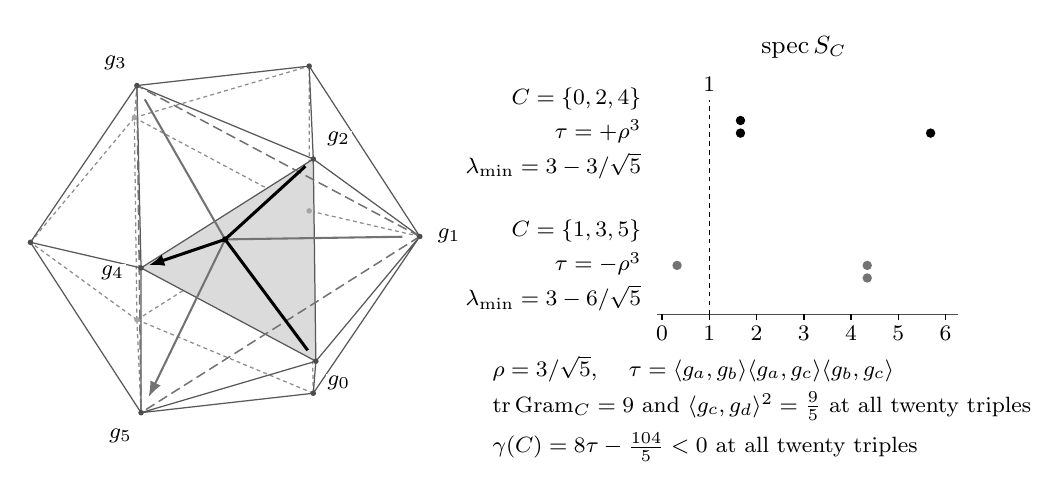
\begin{tikzpicture}[
  x=1cm, y=1cm,
  vec/.style={-{Latex[length=2mm,width=1.5mm]}, line width=0.75pt, black!55},
  heavy/.style={-{Latex[length=2mm,width=1.5mm]}, line width=1.1pt},
  edge/.style={line width=0.45pt, black!65},
  hidden/.style={line width=0.45pt, black!45, dashed,
                 dash pattern=on 1.4pt off 1.2pt},
  chord/.style={line width=0.55pt, black!55, dash pattern=on 3.6pt off 1.8pt},
  tag/.style={font=\footnotesize, fill=white, inner sep=0.6pt},
  every node/.style={font=\small}]

% ---- the twelve vertices, in six antipodal pairs -----------------------
\coordinate (v5)  at ( 1.1526,-1.5469);   % ( 1, phi,  0)
\coordinate (v8)  at (-1.1526, 1.5469);   % (-1,-phi,  0)
\coordinate (v6)  at ( 2.4722, 0.0372);   % (-1, phi,  0)
\coordinate (v7)  at (-2.4722,-0.0372);   % ( 1,-phi,  0)
\coordinate (v1)  at ( 1.1201, 1.0208);   % ( 0,  1, phi)
\coordinate (v4)  at (-1.1201,-1.0208);   % ( 0, -1,-phi)
\coordinate (v2)  at (-1.1201, 1.9539);   % ( 0, -1, phi)
\coordinate (v3)  at ( 1.1201,-1.9539);   % ( 0,  1,-phi)
\coordinate (v9)  at (-1.0676,-0.3623);   % ( phi,  0,  1)
\coordinate (v12) at ( 1.0676, 0.3623);   % (-phi,  0, -1)
\coordinate (v11) at (-1.0676,-2.2008);   % ( phi,  0, -1)
\coordinate (v10) at ( 1.0676, 2.2008);   % (-phi,  0,  1)
\coordinate (O)  at ( 0,0);

% ---- the six atoms, each sigma times the vertex it points at -----------
\coordinate (g0)  at ( 1.0495,-1.4086);   % g_0 = sigma * ( 1, phi,  0)
\coordinate (g1)  at ( 2.2512, 0.0338);   % g_1 = sigma * (-1, phi,  0)
\coordinate (g2)  at ( 1.0200, 0.9295);   % g_2 = sigma * ( 0,  1, phi)
\coordinate (g3)  at (-1.0200, 1.7792);   % g_3 = sigma * ( 0, -1, phi)
\coordinate (g4)  at (-0.9721,-0.3299);   % g_4 = sigma * ( phi,  0,  1)
\coordinate (g5)  at (-0.9721,-2.0040);   % g_5 = sigma * ( phi,  0, -1)

% ---- 12 hidden edges, the face carrying g_0, g_2, g_4, then the 18
% visible edges ---------------------------------------------------------
\draw[hidden]
  (v2)--(v8) (v3)--(v4) (v3)--(v12) (v4)--(v7) (v4)--(v8)
  (v4)--(v11) (v4)--(v12) (v6)--(v12) (v7)--(v8) (v8)--(v10)
  (v8)--(v12) (v10)--(v12);
\path[fill=black!14] (v5)--(v1)--(v9)--cycle;
\draw[edge]
  (v1)--(v2) (v1)--(v5) (v1)--(v6) (v1)--(v9) (v1)--(v10)
  (v2)--(v7) (v2)--(v9) (v2)--(v10) (v3)--(v5) (v3)--(v6)
  (v3)--(v11) (v5)--(v6) (v5)--(v9) (v5)--(v11) (v6)--(v10)
  (v7)--(v9) (v7)--(v11) (v9)--(v11);

% ---- the three chords joining the tips of g_1, g_3, g_5, which bound no
% face --------------------------------------------------------------------
\draw[chord] (v6)--(v2) (v6)--(v11) (v2)--(v11);

% ---- the six atoms as arrows from the centre ---------------------------
\draw[heavy] (O)--(g0) (O)--(g2) (O)--(g4);
\draw[vec]   (O)--(g1) (O)--(g3) (O)--(g5);
\fill (O) circle (1.1pt);
\fill[black!70]
  (v1) circle (1.0pt) (v2) circle (1.0pt) (v3) circle (1.0pt)
  (v5) circle (1.0pt) (v6) circle (1.0pt) (v7) circle (1.0pt)
  (v9) circle (1.0pt) (v10) circle (1.0pt) (v11) circle (1.0pt);
\fill[black!35]
  (v4) circle (1.0pt) (v8) circle (1.0pt) (v12) circle (1.0pt);
\node[tag, anchor=north west] at ( 1.2721,-1.7073) {$g_0$};
\node[tag, anchor=west] at ( 2.6722, 0.0402) {$g_1$};
\node[tag, anchor=south west] at ( 1.2679, 1.1555) {$g_2$};
\node[tag, anchor=south east] at (-1.2196, 2.1274) {$g_3$};
\node[tag, anchor=east] at (-1.2570,-0.4266) {$g_4$};
\node[tag, anchor=north east] at (-1.1549,-2.3807) {$g_5$};

% ---- the two spectra, on one eigenvalue axis; the eigenvalue lambda is
% drawn at abscissa 0.6 lambda -------------------------------------------
\begin{scope}[shift={(5.55,-0.95)}]
  \draw[line width=0.5pt, black!70] (-0.06,0)--(3.7600,0);
  \foreach \lev in {0,1,2,3,4,5,6}{
    \pgfmathsetmacro{\xx}{0.6*\lev}
    \draw[line width=0.5pt] (\xx,0)--(\xx,-0.07);
    \node[anchor=north, font=\footnotesize, inner sep=2pt]
      at (\xx,-0.07) {\lev};}
  \draw[dashed, dash pattern=on 1.7pt off 1.5pt, line width=0.5pt]
        (0.6000,0)--(0.6000,2.7200);
  \node[anchor=south, font=\footnotesize] at (0.6000,2.7000) {$1$};
  \node[anchor=south, font=\small]
    at (1.8000,3.1200) {$\operatorname{spec}\SC$};
  % C = {0,2,4}: spectrum 1.6584, 1.6584, 5.6833
  \fill[black] (0.9950,2.3000) circle (1.7pt);
  \fill[black] (0.9950,2.4600) circle (1.7pt);
  \fill[black] (3.4100,2.3000) circle (1.7pt);
  \node[anchor=east, align=right, font=\footnotesize, inner sep=0pt]
    at (-0.26,2.3000)
    {$C=\{0,2,4\}$\\[3pt] $\tau=+\rho^{3}$\\[3pt] $\lmin=3-3/\sqrt5$};
  % C = {1,3,5}: spectrum 0.3167, 4.3416, 4.3416
  \fill[black!55] (0.1900,0.6200) circle (1.7pt);
  \fill[black!55] (2.6050,0.6200) circle (1.7pt);
  \fill[black!55] (2.6050,0.4600) circle (1.7pt);
  \node[anchor=east, align=right, font=\footnotesize, inner sep=0pt]
    at (-0.26,0.6200)
    {$C=\{1,3,5\}$\\[3pt] $\tau=-\rho^{3}$\\[3pt] $\lmin=3-6/\sqrt5$};
  % what the two rows share
  \node[anchor=north west, align=left, font=\footnotesize, inner sep=0pt]
    at (-2.16,-0.52)
    {$\rho=3/\sqrt5$, \quad $\tau=\langle g_a,g_b\rangle
     \langle g_a,g_c\rangle\langle g_b,g_c\rangle$\\[3.5pt]
     $\tr\Gram_C=9$ and $\langle g_c,g_d\rangle^{2}=\tfrac95$ at
     all twenty triples\\[3.5pt]
     $\gamma(C)=8\tau-\tfrac{104}{5}<0$ at all twenty triples};
\end{scope}
\end{tikzpicture}

  \caption{The icosahedral design at $(6,3)$, in the constants of
  \eqref{eq:icosaconst}: six atoms along the six diagonals of a regular
  icosahedron, each drawn as $\sigma$ times the vertex it points at.  All
  twenty triples carry the trace $9$ and the single pairing modulus
  $\rho$, and ten of them dominate.  The verdict is the sign of the
  product $\tau$ of the three pairings.  The heavy atoms point at the
  vertices of the shaded face, the light ones at three vertices joined by
  no edge.  By Propositions~\ref{prop:icosa} and~\ref{prop:momentsharp} no
  criterion in the trace and the determinant certifies the triple that
  dominates.}
  \label{fig:icosa}
\end{figure}

\subsection{Active-family census at
\texorpdfstring{$(6,3)$ and $(7,3)$}{(6,3) and (7,3)}}\label{app:census}

By \eqref{eq:coverage} the family $A^{+}$ of active $k$-subsets
carrying a positive multiplier covers the index set.  The covering families
of $3$-subsets are counted here up to the symmetric group of the index set
and listed by cardinality.  At $m=6$ a covering family has at
least two members and at most twenty; Table~\ref{tab:census} lists the
counts, whose total is $2102$.  The single class of cardinality two is the
partition branch that Corollary~\ref{cor:e3} leaves undecided; setting
it aside leaves $2101$.  By Proposition~\ref{prop:carath} the support of the
multiplier vector may be taken of size at most $15$ here, so only the columns
up to $15$ bear on
Conjecture~\ref{conj:sixthree}; they account for $2069$ of the $2102$ classes,
and for $2068$ of the $2101$ with at least three members.

At $m=7$ a covering family has at least three members, and the counts are
\[
\begin{array}{c|cccccccc}
\lvert A^{+}\rvert & 3&4&5&6&7&8&9&10\\ \hline
\text{classes} & 3&17&94&415&1599&5308&15397&39081\\[4pt]
\lvert A^{+}\rvert & 11&12&13&14&15&16&17&18\\ \hline
\text{classes} & 87347&172684&303116&473733&660907&824389&920439&920443\\[4pt]
\lvert A^{+}\rvert & 19&20&21&22&23&24&25&26\\ \hline
\text{classes} & 824409&660949&473827&303277&172933&87659&39433&15709\\[4pt]
\lvert A^{+}\rvert & 27&28&29&30&31&32&33&34\\ \hline
\text{classes} & 5557&1760&509&137&38&10&3&1
\end{array}
\]
together with a single class of cardinality $35$,
with total $7\,011\,184$.  By Proposition~\ref{prop:carath} the bound at
$(7,3)$ is $19$, and the classes of cardinality at most
$19$ already number $5\,249\,381$.  Enumeration at this size is not a route;
Problem~\ref{prob:seventhree} asks instead for an argument uniform in
the active family.


\bibliographystyle{amsplain}
\bibliography{refs}

\end{document}
